\documentclass[a4paper, german, lecturenumbers = true, number small environments = theorem]{mkessler-script}

\course{Einführung in die Geometrie und Topologie}
\lecturer{Daniel Kasprowski}
\assistant[f]{Arunima Ray}
\author{Maximilian Keßler}

\RequirePackage{mkessler-math}
\RequirePackage{mkessler-fancythm}
\usepackage{epsfig}
%\usepackage{psfrag}
%\usepackage{sseq} (if you need to draw spectral sequences, please use this package, available at http://wwwmath.uni-muenster.de/u/tbauer/)
\usepackage{mathrsfs}
\usepackage{amscd}
\usepackage{amsbsy}
\usepackage{verbatim}
\usepackage{moreverb}

\newtheorem{prop}[theorem]{Proposition}
\newtheorem{cor}[theorem]{Corollary}
\newtheorem{conj}[theorem]{Conjecture}


\theoremstyle{definition}
\newtheorem{hw}{Homework}
\newtheorem{exercise*}[exercise]{$\star$ Exercise}

\theoremstyle{remark}
\newtheorem{aside}[theorem]{Aside}

\newcommand{\nn}{\nonumber}
\newcommand{\nid}{\noindent}
\newcommand{\ra}{\rightarrow}
\newcommand{\la}{\leftarrow}
\newcommand{\xra}{\xrightarrow}
\newcommand{\xla}{\xleftarrow}
\newcommand{\tto}{\longrightarrow}

\newcommand{\weq}{\xrightarrow{\sim}}
\newcommand{\cofib}{\rightarrowtail}
\newcommand{\fib}{\twoheadrightarrow}

\newcommand{\IRep}{\mathrm{IRep}}
\newcommand{\IHom}{\mathrm{IHom}}

\def\llarrow{   \hspace{.05cm}\mbox{\,\put(0,-2){$\leftarrow$}\put(0,2){$\leftarrow$}\hspace{.45cm}}}
\def\rrarrow{   \hspace{.05cm}\mbox{\,\put(0,-2){$\rightarrow$}\put(0,2){$\rightarrow$}\hspace{.45cm}}}
\def\lllarrow{  \hspace{.05cm}\mbox{\,\put(0,-3){$\leftarrow$}\put(0,1){$\leftarrow$}\put(0,5){$\leftarrow$}\hspace{.45cm}}}
\def\rrrarrow{  \hspace{.05cm}\mbox{\,\put(0,-3){$\rightarrow$}\put(0,1){$\rightarrow$}\put(0,5){$\rightarrow$}\hspace{.45cm}}}

\def\cA{\mathcal A}\def\cB{\mathcal B}\def\cC{\mathcal C}\def\cD{\mathcal D}
\def\cE{\mathcal E}\def\cF{\mathcal F}\def\cG{\mathcal G}\def\cH{\mathcal H}
\def\cI{\mathcal I}\def\cJ{\mathcal J}\def\cK{\mathcal K}\def\cL{\mathcal L}
\def\cM{\mathcal M}\def\cN{\mathcal N}\def\cO{\mathcal O}\def\cP{\mathcal P}
\def\cQ{\mathcal Q}\def\cR{\mathcal R}\def\cS{\mathcal S}\def\cT{\mathcal T}
\def\cU{\mathcal U}\def\cV{\mathcal V}\def\cW{\mathcal W}\def\cX{\mathcal X}
\def\cY{\mathcal Y}\def\cZ{\mathcal Z}

\def\sA{\mathscr A}\def\cB{\mathcal B}\def\cC{\mathcal C}\def\cD{\mathcal D}
\def\cE{\mathcal E}\def\cF{\mathcal F}\def\sG{\mathscr G}\def\cH{\mathcal H}
\def\cI{\mathcal I}\def\cJ{\mathcal J}\def\cK{\mathcal K}\def\cL{\mathcal L}
\def\cM{\mathcal M}\def\cN{\mathcal N}\def\cO{\mathcal O}\def\cP{\mathcal P}
\def\cQ{\mathcal Q}\def\cR{\mathcal R}\def\cS{\mathcal S}\def\cT{\mathcal T}
\def\cU{\mathcal U}\def\cV{\mathcal V}\def\cW{\mathcal W}\def\cX{\mathcal X}
\def\cY{\mathcal Y}\def\cZ{\mathcal Z}

\def\fG{\mathfrak G}\def\fH{\mathfrak H}
\def\fS{\mathfrak S}\def\fN{\mathfrak N}\def\fX{\mathfrak X}\def\fY{\mathfrak Y}

\def\op{\textrm{op}}\def\ob{\textrm{ob}}

%\def\Iso{\mathcal Iso}\def\cInn{\mathcal Inn}

\def\fg{\mathfrak g}\def\fh{\mathfrak h}\def\fri{\mathfrak i}\def\fp{\mathfrak p}
\def\fA{\mathfrak A}\def\fU{\mathfrak U}

\def\AA{\mathbb A}\def\BB{\mathbb B}\def\CC{\mathbb C}\def\DD{\mathbb D}
\def\EE{\mathbb E}\def\FF{\mathbb F}\def\GG{\mathbb G}\def\HH{\mathbb H}
\def\II{\mathbb I}\def\JJ{\mathbb J}\def\KK{\mathbb K}\def\LL{\mathbb L}
\def\MM{\mathbb M}\def\NN{\mathbb N}\def\OO{\mathbb O}\def\PP{\mathbb P}
\def\QQ{\mathbb Q}\def\RR{\mathbb R}\def\SS{\mathbb S}\def\TT{\mathbb T}
\def\UU{\mathbb U}\def\VV{\mathbb V}\def\WW{\mathbb W}\def\XX{\mathbb X}
\def\YY{\mathbb Y}\def\ZZ{\mathbb Z}

\def\TOP{\mathcal{TOP}}\def\GRP{\mathcal{GRP}}\def\GRPD{\mathcal{GRPD}} \def\CAT{\mathcal{CAT}} \def\SET{\mathcal{SET}}

\def\id{\mathrm{id}}\def\Id{\mathrm{Id}}
\def\inverse{^{-1}}


\setuptodonotes{disable}


\begin{document}
    \maketitle

    \abstract{Bei folgenden Vorlesungsnotizen handelt es sich um (inoffizielle) Mitschriften zur Vorlesung 'Algorithmische Mathematik II', die im Sommersemester 2021 an der Universität Bonn gehalten wird. Ich garantiere weder für Korrektheit noch Vollständigkeit dieser Notizen, und bin dankbar für jegliche Art von Korrektur, sowohl inhaltlich, als auch Tippfehler. \\
Bemerkungen, die nicht zum eigentlichen Vorlesungsinhalte gehören, wurden mit einem * gekennzeichnet. Sie werden nach eigenem Ermessen hinzugefügt, um weitere Details oder evtl. mündliche Anmerkungen beizufügen. \\
Manche Umgebungen sind mit einem $^{\dagger}$ versehen. Das ist dann der Fall, wenn ihr Inhalt so, oder zumindest in sehr ähnlicher Form, in der Vorlesung vorkam (unter Umständen auch mündlich), ich aber die Umgebung der Aussage geändert habe. Das ist z.B. dann der Fall, wenn ich aus Aussagen, die einfach erwähnt werden, ein \textbf{Lemma$^{\dagger}$} mache, um sie hervorzuheben. \\
Weitere Informationen finden sich bei \href{https://github.com/kesslermaximilian/LectureNotesBonn}{GitHub} oder auf der \href{https://wt.iam.uni-bonn.de/ferrari/teaching/lectures-homepages/almaiiss19-1}{Vorlesungshomepage}


    %Table of contents
    \cleardoublepage
    \tableofcontents

    %List of lectures with their corresponding keywords
    \cleardoublepage
    \summaryoflectures

    \cleardoublepage
    % start lectures
    %! TEX root = ./master.tex
\lecture[Metrische Räume. Umgebungen, offene Mengen, Stetigkeit. Topologische Räume. Metrisierbarkeit.]{Di 13 Apr 2021 12:16}{Einführung}
\begin{orga}
\begin{itemize}
\item    Die Vorlesung wird aufgezeichnet.
\item Wir duzen uns.
\item Für die Übungen muss man sich auf eCampus anmelden, ob Do, 20:00 Uhr (Do 15 Apr 2021 20:00 Uhr)
\item Die Übungsblätter werden Donnerstag zur Verfügung gestellt und werden nach 10 Tagen am Montag, 10 Uhr abgegeben.
\item Es wird eine Fragestunde um Donnerstag, 16 Uhr geben.
\item Es wird kein Skript geben, allerdings werden die geschriebenen Notizen auf eCampus zur Verfügung gestellt.
\item Die Vorlesung orientiert sich an der vom letzten Jahr.
\item Für Literatur sind empfohlen: \cite{topology-waldhausen}, \cite{algebraic-topology-hatcher} sowie \cite{topology-and-geometry} (auch auf der Vorlesungshomepage zu finden).
\end{itemize}
\end{orga}

\setcounter{section}{-1}

\section{Motivation und Überblick}
In der Topologie studieren wir topologische Räume. Diese verallgemeinern metrische Räume. Wir wollen zwei metrische Räume $X,Y$ als 'gleich' ansehen, wenn es stetige, zueinander inverse Abbildungen  $X \to  Y, Y\to X$ gibt.
\begin{example}
    Betrachte ein Quadrat und einen Kreis, wir können sie durch Streckung aufeinander abbilden. Gleiches gilt für eine Tasse und einen Donut. \\
    \begin{minipage}{\textwidth}
    \centering
    \begin{minipage}{0.45\textwidth}
     \incfig{quadrat-und-kreis-sind-gleich}
    \end{minipage}
    \begin{minipage}{0.45\textwidth}
    \incfig{tasse-und-donut-sind-gleich}
    \end{minipage}
    \captionof{figure}{Beispiele 'gleicher' metrischer Räume (homöomorph)}
\end{minipage}
\end{example}




\begin{idea}
    Räume sind gewissermaßen aus 'Knete'.
\end{idea}
\begin{goal}
    Wann sind zwei Räume gleich?
\end{goal}
Dazu werden wir algebraische Invarianten verwenden.
\begin{example}
    $\R^n$ und $\R^m$ sind nicht 'gleich' für $n\neq m$.
\end{example}
Der Aufbau ist wie folgt:
\begin{description}
    \item[1. Teil] Grundlagen
    \item[2. Teil] erste Invarianten: Fundamentalgruppe (dazu Überlagerungen)
\end{description}


\newpage
\part{Mengentheoretische Topologie}

\section{Metrische Räume}
\begin{definition}[Metrik]\label{def:metrik}
    Eine \vocab[Metrik]{Metrik} auf einer Menge $X$ ist eine Funktion  $d: X\times X \to  \R_{\geq 0}$ mit folgenden Eigenschaften:
    \begin{enumerate}[(i)]
        \item $d(x,y) = 0 \iff  x = y$
        \item $d(x,y) = d(y,x) \quad \forall x,y\in X$
        \item (Dreiecksungleichung) $d(x,z) \leq  d(x,y) + d(y,z)$.
    \end{enumerate}
    Ein \vocab{Metrischer Raum} ist ein Paar $(X,d)$ aus einer Menge $X$ und einer Metrik $d$ auf $X$.
\end{definition}

\begin{definition}[Stetigkeit]\label{def:stetig-metrischer-raum}
    Seien $(X,d)$ und  $(X',d')$ zwei metrische Räume. Dann ist eine Funktion $f:X \to  Y$ \vocab[Stetig!in $x\in X$]{stetig in $x\in X$}, falls
    \[
        \forall ε > 0 \; \exists \delta > 0 \; \forall x' \colon d(x,x') < \delta \implies d'(f(x), f(x')) < ε
    .\] 
    Eine Funktion $f$ heißt \vocab[Stetig]{stetig}, wenn sie in jedem Punkt  $x\in X$ stetig ist.
    \begin{minipage}{\textwidth}
        \centering
    \incfig{definition-von-stetigkeit-in-metrischen-raeumen}
    \captionof{figure}{Definition von Stetigkeit in metrischen Räumen}
    \end{minipage}
\end{definition}


\begin{example}
    \begin{itemize}
        \item 
    Sei $V$ ein reeller Vektorraum mit Norm  $\lVert \cdot  \rVert$. Dann definiert
    \[
        d(v,w) := \lVert v-w \rVert 
    .\] 
    eine Metrik auf $V$. Insbesondere ist $\R^n$ mit euklidischer Norm
    \[
        \lVert (x_1,\ldots,x_n) \rVert _2 = \sqrt{x_1^2 + \ldots + x_{n}^2} 
    .\] 
    dadurch ein metrischer Raum.
\item Ist $(X,d)$ ein metrischer Raum und  $Y\subset X$ eine Teilmenge, dann ist $(Y, d| _{Y\times Y})$ ein metrischer Raum.
\item Sei $X$ eine Menge. Dann ist
    \[
        d(x,y) = \begin{cases}
            0 & \text{falls } x=y \\
            1 & \text{sonst}
        \end{cases}
    .\] 
    eine Metrik auf $X$, genannt die \vocab[Metrik!diskrete]{diskrete Metrik}.
    \end{itemize}
\end{example}
\begin{notation}
    Sei $X$ ein metrischer Raum. Für  $x\in X$ und $ε>0$ setzen wir
     \[
         U(x,ε) := \left \{y\in X \mid  d(x,y) < ε\right\} 
    .\] 
    und nennen dies den \vocab[Offener $ε$-Ball um  $x$]{offenen $ε$-Ball um $x$}
\end{notation}
\begin{observe}
    Sei $f: (X,d_X) \to  (Y,d_Y)$ eine Funktion, $x\in X$ sowie $ε,δ>0$. Dann sind äquivalent:
\begin{enumerate}[1)]
    \item $\forall x' \in X$ mit $d_X(x',x) < δ$ gilt  $d_Y(f(x'),f(x)) < ε$
    \item Es ist $f(U(x,\delta)) \subset U(f(x),ε)$
    \end{enumerate}
\end{observe}
\begin{definition}[Umgebung]\label{def:umgebung-metrischer-raum}
    Sei $X$ ein metrischer Raum,  $U\subset X$ und $x\in X$. Dann heißt $U$ \vocab[Umgebung]{Umgebung von $x$}, falls ein $ε>0$ existiert, sodass  $U(x,ε) \subset U$. 
\end{definition}
\begin{theorem}[Urbilder von Umgebungen]\label{thm:stetig-gdw-urbild-von-umgebung-ist-umgebung}
    Sei $f:X \to  Y$ eine Abbildung zwischen metrischen Räumen und sei $x\in X$. Dann ist $f$ stetig in  $x$ genau dann, wenn für alle Umgebungen  $V$ um  $f(x)$ in  $Y$ das Urbild  $f^{-1}(V)$ eine Umgebung von $x$ ist.
\end{theorem}

\begin{proof}
'$\implies$' Sei $V$ eine Umgebung von  $f(x)$. Dann  $\exists \; ε>0$ mit $U(f(x),ε) \subset V\}$. Da $f$ stetig ist,  $\exists \; δ>0$, sodass $f(X(x,δ)) \subset U(f(x),ε)\subset V$. Also ist $U(x,δ)\subset f^{-1}(V)$ und somit ist $f^{-1}(V)$ eine Umgebung von $x$. \\
'$\impliedby$'.  Sei $ε>0$. Dann ist  $U(f(x),ε)$ eine Umgebung von  $f(x)$. Also ist  $f^{-1}(U(f(x),ε))$ eine Umgebung von $x$, also  $\exists \; δ>0$ mit $U(x,δ) \subset f^{-1}(U(f(x),ε))$. Also wie gewünscht $f(U(x,δ)) \subset U(f(x),ε))$.
\end{proof}

\begin{definition}[Offene Mengen]\label{def:offene-menge-metrischer-raum} 
    Sei $X$ ein metrischer Raum. Eine Teilmenge  $U\subset X$ heißt \vocab[Metrischer Raum!offene Menge]{offen}, falls sie Umgebung all ihrer Punkte ist, d.h. $\forall x\in U \;\exists ε>0$ mit $U(x,ε)\subset U$.
\end{definition}
\begin{remark}
    $U(x,ε)$ ist offen.
\begin{proof}
    Für alle $y\in U(x,ε)$ ist
    \[
        U(y, \underbrace{ε - d(x,y)}_{>0}) \subset U(x,ε)
    .\] 
    nach der Dreiecksungleichung.
\end{proof}
\end{remark}

\begin{theorem}[Urbilder offener Mengen sind offen]\label{thm:urbild-offener-menge-ist-offen}
    Eine Abbildung $f:X\to Y$ zwischen metrischen Räumen ist stetig genau dann, wenn $\forall U \subset Y \text{  offen}$ auch das Urbild $f^{-1}(U)$ offen in $X$ ist.
\end{theorem}
\begin{proof}
    '$\implies$ '. Sei $U\subset Y$ eine offene Teilmenge und $x\in f^{-1}(U)$ beliebig. Dann ist $f(x) \in U$ und somit ist $U$ eine Umgebung von  $f(x)$. Da  $f$ stetig ist, ist  $f^{-1}(U)$ eine Umgebung von $x$ nach \autoref{thm:stetig-gdw-urbild-von-umgebung-ist-umgebung}. Also ist $f^{-1}(U)$ offen, da $x$ beliebig war.\\
    '$\impliedby$' Sei $x\in X$, $V$ eine Umgebung von  $f(x)$. Dann  $\exists ε>0$ mit $U(f(x),ε)\subset V$. Nach Annahme ist $f^{-1}(U(f(x),ε))$ offen. Also gibt es ein $δ>0$ mit  $U(x,δ) \subset f^{-1}(U(f(x),ε))\subset f^{-1}(V)$. Also ist $f^{-1}(V)$ eine Umgebung von $x$. \\
    Damit ist  $f$ stetig nach \autoref{thm:stetig-gdw-urbild-von-umgebung-ist-umgebung}
\end{proof}

\begin{theorem}[Offene Mengen in metrischen Räumen]\label{thm:offene-mengen-in-metrischem-raum}
    Sei $X$ ein metrischer Raum. Dann gilt:
    \begin{enumerate}[1)]
        \item Die leere Menge $\emptyset$ und $X$ sind offen
        \item  $\forall U_1,\ldots,U_n\subset X$ offen ist auch $\bigcap_{i=1}^n U_i$ offen.
        \item Für jede Familie $\left \{U_i\right\} _{i\in I}$ von offenen Mengen ist auch $\bigcup_{i\in I} U_i$ offen.
    \end{enumerate}
\end{theorem}
\begin{warning}
    Eigenschaft $2)$ gilt nicht für unendliche Schnitte. Es ist $\left( -\frac{1}{n},\frac{1}{n} \right) \subset \R$ offen für alle $n\in \N_{>0}$, allerdings ist dann
    \[
        \bigcap_{n\in \N_{>0}} \left( -\frac{1}{n},\frac{1}{n} \right)  = \left \{0\right\} 
    .\] 
    nicht offen.
\end{warning}

\begin{proof}[Beweis von \autoref{thm:offene-mengen-in-metrischem-raum}]
    \begin{enumerate}[1)]
        \item klar
        \item Sei $x\in \bigcap_{i=1}^n U_i$. $\forall i = 1,\ldots,n$ gibt es nun $ε_i$ mit  $U(x,ε_i)\subset U_i$. Setze $ε := \min \left \{ε_i \mid  i=1,\ldots,n\right\}$. Dann ist
            \[
                U(x,ε) \subset U(x,ε_i) \subset U_i
            .\] 
            für alle $i=1,\ldots,n$ und somit wie gewünscht $U(x,ε) \subset \bigcap_{i=1}^n U_i$
        \item Sei $x\in \bigcup_{\in I} U_i$ beliebig. Dann $\exists i\in I$ mit $x\in U_i$. Da $U_i$ offen ist,  $\exists ε>0$ mit $U(x,ε) \subset U_i$. Also ist $U(x,ε) \subset  \bigcup_{i\in I} U_i$ und somit ist die Vereinigung offen.
    \end{enumerate}
\end{proof}

\section{Topologische Räume} 
    
\begin{definition}[Topologie]\label{def:topologie}
    Eine \vocab{Topologie} auf einer Menge $X$ ist eine Menge  $\mathcal{O}$ von Teilmengen von  $X$, so dass gilt:
    \begin{enumerate}[1)]
        \item $\emptyset,X \in \mathcal{O}$
        \item Für $U_1,\ldots,U_n \in \mathcal{O}$ ist auch $\bigcap_{i=1}^n U_i \in  \mathcal{O}$
        \item Für jede Familie $\left \{U_i\right\} _{i\in I}$ mit $U_i \in \mathcal{O}$ ist auch $\bigcup_{i\in I} U_i \in  \mathcal{O}$
    \end{enumerate}
    Die Mengen in $\mathcal{O}$ heißen \vocab[Menge!offen]{offene Mengen}. \\
    Ein \vocab[Topologischer Raum]{topologischer Raum} ist ein Paar  $(X,\mathcal{O})$ aus einer Menge  $X$ und einer Topologie  $\mathcal{O}$ auf  $X$.
\end{definition}


\begin{definition}[Stetigkeit]\label{def:stetig}
    Seien $X,Y$ topologische Räume. Eine Abbildung  $f:X \to  Y$ heißt \vocab[Stetig]{stetig}, falls für jede offene Teilmenge $U\subset Y$ das Urbild $f^{-1}(U) \subset X$ offen ist.
\end{definition}

\begin{example}
    Sei $(X,d)$ ein metrischer Raum. Dann ist
     \[
         (X, \mathcal{O}) := \left \{U\subset X \mid  U \text{ ist offen bezüglich $d$}\right\} 
    .\] 
    ein topologischer Raum. $\mathcal{O}$ ist die von der Metrik  $d$ \vocab[Topologie!induzierte]{induzierte Topologie}.
\end{example}

\begin{definition}[Metrisierbarkeit]\label{def:metrisierbar}
    Ein topologischer Raum heißt \vocab[Topologischer Raum!metrisierbar]{metrisierbar}, falls die Topologie von einer Metrik induziert ist.
\end{definition}

\begin{example}
    Sei $X$ eine Menge. Die \vocab[Topologie!diskrete]{diskrete Topologie} auf $X$ ist die Menge aller Teilmengen, d.h.  $\mathcal{O} := \mathcal{P}(X)$. Diese ist von der diskreten Metrik
    \[
        d(x,y) = \begin{cases}
            0 & \text{falls }x=y \\
            1 & \text{sonst}
        \end{cases}
    .\] 
    induziert.
\end{example}
\begin{proof}
    Ist $x\in X$, dann ist
    \[
        \left \{x\right\} =U\left(x,\frac{1}{2}\right)
    .\] 
    offen. Ist $U\subset X$ eine Teilmenge, dann ist
    \[
    U = \bigcup_{x\in U} \left \{x\right\}
    .\] 
    offen als Vereinigung offener Mengen.
\end{proof}

\begin{theorem}\label{thm:endlicher-metrisierbarer-raum-ist-diskret}
    Sei $X$ ein endlicher (endlich als Menge), metrisierbarer topologischer Raum. Dann ist  $X$ diskret (d.h. $X$ trägt die diskrete Topologie).
\end{theorem}
\begin{proof}
    Es reicht zu zeigen, dass $\left \{x\right\} $ offen ist $\forall x\in X$. Sei $d$ eine Metrik, die die Topologie induziert, dann wähle
     \[
         ε := \min \left \{d(x,y) \mid  x,y\in X , x\neq y\right\} > 0
    .\] 
    Beachte, dass dies existiert, da $d(x,y) >0$ für  $x\neq y$ und die Menge nach Voraussetzung endlich ist. Nun ist:
    \[
    \left \{x\right\}  = U(x,ε)
    .\] 
    offen und wir sind fertig.
\end{proof}

\begin{example}
    \begin{enumerate}[1)]
        \item Wähle $X = \left \{a,b\right\} $ und setze
            \[
            \mathcal{O} = \left \{\emptyset,X, \left \{a\right\} \right\} 
            .\]
            Dies ist ein topologischer Raum (leicht prüfen), er ist jedoch nicht metrisierbar, da endlich und nicht diskret. Dieser Raum heißt \vocab{Sierpinski-Raum}. 
        \item Sei $X$ eine Menge. Die  \vocab[Topologie!indiskrete]{indiskrete Topologie} auf $X$ enthält nur  $\emptyset,X$. Man prüft leicht, dass dies eine Topologie ist. 
            \begin{itemize}
                \item 
            Hat $X$ mindestens 2 Elemente, so ist  $X$ nicht metrisierbar.
             \begin{proof}
                 Nimm $\abs{X}>2$ an und wähle $x,y\in X$ mit $x\neq y$. Sei $d$ eine Metrik, die die Topologie auf $X$ induziert und setze  $ε := d(x,y)$. Dann ist
                  \[
                      x\in U(x,ε) \quad y\not\in U(x,ε)
                 .\] 
                 also ist $U(x,ε) \neq  \emptyset,X$, Widerspruch.
            \end{proof}
        \item Sei $Y$ ein topologischer Raum. Dann ist  $f: Y \to  X$ stetig für beliebige Abbildungen $f$.
             \begin{proof}
                 Es sind $f^{-1}(\emptyset) = \emptyset$ sowie $f^{-1}(X) = Y$ beide offen.
            \end{proof}
            \end{itemize}
    \end{enumerate}    
\end{example}

\begin{remark}
    Ist $Y$ diskret und  $X$ beliebig, so ist jede Abbildung  $f:Y \to  X$ stetig.
\end{remark}










    %! TEX root = ./master.tex
\lecture[\"Aquivalente Metriken. Abgeschlossene Mengen. Teilraumtopologie. Hom\"oomorphismen. Quotientenräume und -topologie.]{Do 15 Apr 2021 10:14}{Grundbegriffe}


\begin{definition}[Äquivalente Metriken]\label{def:äquivalente-metrik}
    Zwei Metriken $d_1,d_2$ auf $X$ heißen \vocab[Metrik!äquivalente]{äquivalent}, falls Konstanten $c_1,c_2$ existieren, sodass
    \[
        \forall x,y\in X \colon \quad c_1\cdot d_1(x,y) \leq  d_2(x,y) \leq  c_2\cdot d_1(x,y)
    .\] 
\end{definition}
\begin{theorem}\label{thm:äquivalenz-von-metriken-ist-äquivalenzrelation}
    Äquivalenz (von Metriken) ist eine Äquivalenzrelation.
\end{theorem}
\begin{proof}
    \begin{description}
        \item[Reflexivität:] Klar mit $c_1 = c_2 = 1$
        \item[Symmetrie:] Seien $c_1,c_2$ wie in der Definition. Dann gilt mit entsprechender Division, dass
            \[
                \forall x,y \in X \colon : \quad \frac{1}{c_2}\cdot d_2(x,y) \leq  d_1(x,y) \leq  \frac{1}{c_1}d_2(x,y)
            .\] 
        \item[Transitivität:]. Seien $c_1,c_2,c_1',c_2'$ gewählt, sodass $\forall x \; \forall y\colon c_1d_1 (x,y) \leq  d_2 (x,y)\leq  c_2d_1(x,y)$ sowie $c_1'd_2 (x,y)\leq  d_3(x,y) \leq  c_2'd_2(x,y)$ (Also $d_1 \sim  d_2$ und $d_2 \sim d_3$). Dann ist auch
            \[
\forall x \; \forall y \colon \quad                c_1c_1'd_1(x,y) \leq  c_1'd_2(x,y)\leq d_3(x,y) \leq  c_2'd_2 (x,y) \leq  c_2d_1(x,y)
            .\] 
    \end{description}
\end{proof}

\begin{theorem}\label{thm:äquivalente-metriken-erzeugen-dieselbe-topologie}
    Äquivalente Metriken induzieren dieselbe Topologie.
\end{theorem}
\begin{proof}
    Wegen der Symmetrie genügt es zu zeigen, dass Mengen, die offen bezüglich $d_2$ sind, auch offen bezüglich $d_1$ sind. \\
    Sei nun $U\subset X$ offen bezüglich $d_2$ und $x\in U$. Dann existiert ein $ε>0$ mit  $U_{d_2}(x,ε) \subset U$. Ist nun $d_1(x,y) < \frac{ε}{c_2}$, dann ist
    \[
        d_2(x,y) \leq  c_2d_1(x,y) < ε
    .\] 
und damit ist
\[
    U_{d_1}\left(x,\frac{ε}{c_2}\right) \subset U_{d_2} \left( x,ε \right) \subset U
.\] 
und somit ist $U$ auch offen bezüglich  $d_1$.
\end{proof}

\begin{remark}
    Es gibt auch nicht-äquivalente Metriken, die die gleiche Topologie induzieren. Siehe hierzu \autoref{aufgabe-1.2}.
\end{remark}
\begin{remark}
    Je zwei Normen auf $\R^n$ sind äquivalent, induzieren also dieselbe Topologie, das beweisen wir jedoch hier nicht.
\end{remark}

\begin{definition}[Umgebung]\label{def:umgebung}
    Sei $X$ ein topologischer Raum und $U\subset X$ sowie $x\in X$. Dann heißt $U$ \vocab[Umgebung!von $x$]{Umgebung von $x$}, falls es eine offene Teilmenge  $O\subset X$ gibt, mit $x\in O\subset U$.
\end{definition}
\begin{remark}
    Für metrische Räume stimmt dies mit der vorherigen Definiton überein.
\end{remark}


\begin{theorem}\label{thm:offene-menge-ist-umgebung-all-ihrer-punkte}
    Sei $X$ ein topologischer Raum und  $U\subset X$. Dann sind äquivalent:
    \begin{enumerate}[1)]
        \item $U$ ist offen.
        \item $U$ ist Umgebung aller ihrer Punkte.
    \end{enumerate}
\end{theorem}
\begin{proof}
    '$1) \implies 2)$' ist klar, wähle einfach $O = U$. \\
    '$2)\implies_1)$'. Für jedes $x\in U$ existiert also $U_x$ mit  $x\in U_x \subset U$. Dann ist aber
    \[
    U = \bigcup_{x\in U} U_x
    .\] 
    offen als Vereinigung offener Mengen.
\end{proof}

\begin{definition*}[Abgeschlossene Mengen]\label{def:abgeschlossene-menge}
    Sei $X$ ein topologischer Raum. Eine Teilmenge  $A\subset X$ heißt \vocab[Menge!abgeschlossen]{abgeschlossen}, falls ihr Komplement $X \setminus A = \left \{x\in X \mid  x\not\in A\right\} $ offen ist.
\end{definition*}
\begin{remark}
    Für metrische Räume stimmt das mit dem Begriff aus der Analysis überein.
\end{remark}

\begin{theorem}[Dualität]\label{offen-abgeschlossen-ist-dual}
    Ein topologischer Raum lässt sich auch über seine abgeschlossenen Mengen charakterisieren. Diese müssen erfüllen:
    \begin{enumerate}[i)]
        \item $\emptyset,X$ sind abgeschlossen
        \item Für $A_1,\ldots,A_n$ abgeschlossen ist auch $A_1\cup \ldots \cup A_n$ abgeschlossen.
        \item Für eine Familie $\left \{A_i\right\} _{\in I}$ abgeschlossener Mengen ist auch
            \[
            \bigcap_{i\in I} A_i
            .\] 
            abgeschlossen.
    \end{enumerate}
\end{theorem}

\begin{recap}
    Wenn wir von einer Familie von Mengen $\left \{A_i\right\} _{\in I}$ sprechen, meinen wir, dass $I$ eine Menge ist, und für jedes $\in I$ ist $A_i$ eine Teilmenge von  $X$. Formal können wir dies als eine Funktion  $I \to  \mathcal{P}(X)$ darstellen.
\end{recap}
\begin{proof}[Beweis von \autoref{offen-abgeschlossen-ist-dual}]
    \begin{enumerate}[i)]
        \item $X \setminus \emptyset = X$, $X\setminus X = \emptyset$ sind abgeschlossen.
        \item  \[
                \underbrace{\bigcap_{i=1}^n (X\setminus A_i)}_{\text{offen}} = X \setminus  \bigcup_{i=1}^n A_i \quad \implies \bigcup_{i=1}^n A_i \text{ abgeschlossen}
        .\] 
        \item \[
                \underbrace{\bigcup_{i\in I} (\underbrace{X\setminus A_i}_{\text{offen}})}_{\text{offen}} = X \setminus \bigcap_{i \in I} A_i \quad \implies \bigcap_{i \in I} A_i \text{ abgeschlossen}
        .\] 
    \end{enumerate}
\end{proof}

\begin{theorem}[Stetigkeit mit abgeschlossenen Mengen]\label{thm:stetig-gdw-urbilder-abgeschlossener-mengen-sind-abgeschlossen}
    Sei $f:X \to  Y$ eine Funktion zwischen topologischen Räumen. Dann sind äuqivalent:
    \begin{enumerate}[1)]
        \item $f$ ist stetig
        \item $\forall U\subset Y$ offen ist $f^{-1}(U) \subset X$ offen
        \item  $\forall A\subset Y$ abgeschlossen ist $f^{-1}(A)$ abgeschlossen
    \end{enumerate}
\end{theorem}
\begin{proof}
    \begin{equation*}
        \begin{split}
            f \text{ stetig} &\iff \forall U \subset  Y \text{ offen ist } f^{-1}(U) \text{ offen}  \\
                             &\iff  \forall A \subset Y \text{ abgeschlossen ist } f^{-1}(Y \setminus A) \text{ offen} \\
                             &\iff \forall A\subset Y \text{ abgeschlossen ist } X \setminus f^{-1}(A) \text{ offen} \\
                             &\iff  \forall A\subset Y \text{ abgeschlossen ist } f^{-1}(A) \text{ abgeschlossen}
        \end{split}
    \end{equation*}
\end{proof}


Wir erinnern uns: Ist $(X,d)$ ein metrischer Raum, so auch  $\left(Y, d_{Y\times Y}\right) \quad \forall Y\subset X$. Wie ist dies für topologische Räume?
\begin{warning}
    $(Y, \mathcal{O}_X \cap \mathcal{P}(Y))$ ist im allgemeinen \textbf{kein} topologischer Raum. (wenn $Y$ nicht offen ist, denn dann ist $Y\not\in \mathcal{S}_X \cap \mathcal{P}(X)$)
\end{warning}
\begin{theoremdef}[Teilraumtopologie]\label{def:teilraumtopologie}
    Sei $X$ ein topologischer Raum,  $Y\subset X$. Dann ist
    \[
    \mathcal{O}_Y := \left \{U \cap Y \mid  U\subset X \text{ offen}\right\} 
    .\] 
    eine Topologie auf $Y$, die  \vocab[Topologie!Teilraum-]{Teilraumtopologie} oder auch \vocab[Topologie!Unterraum-]{Unterraumtopologie} genannt wird.  
\end{theoremdef}

\begin{example}
    Betrachte $\R^1 \subset \R^2$ als Unterraum. Schneiden wir eine offene Menge in $\R^2$ mit $\R^1$, so erhalten wir ein offenes Intervall: \\
\begin{minipage}{\textwidth}
\centering    
    \incfig{r1-als-unterraum-von-r2}
    \captionof{figure}{$\R^1$ als Unterraum von $\R^2$}
\end{minipage}
\end{example}
\begin{proof}
    \begin{itemize}
        \item Es sind $\emptyset = \emptyset \cap Y$ und $Y = X \cap Y$ offen.
        \item Es ist 
            \[
                \bigcap_{i=1}^n \left( U_i \cap Y \right)  = \left( \bigcap_{i=1}^n U_i \right)  \cap Y
            .\] 
        \item Es ist
            \[
                \bigcup_{i\in I} \left( U_i \cap Y \right) = \left( \bigcup_{i \in  I} U_i \right) \cap Y
            .\] 
    \end{itemize}
\end{proof}
\begin{warning}
    Für $Z\subset Y\subset X$ muss man zwischen 'offen in $Y$' und  'offen in  $X$' unterscheiden, falls  $Y$ nicht offen ist.
\end{warning}
\begin{remark*}
    Ist $Y\subset X$ offen, so stimmen die beiden vorherigen Konzepte tatsächlich überein, d.h. eine Menge $Z\subset Y$ ist offen in $Y$, genau dann, wenn sie offen in  $X$ ist.
\end{remark*}

\begin{remark}
    Sei $(X,d)$ ein metrischer Raum und  $Y\subset X$ eine Teilmenge. Die Unterraumtopologie auf $Y$ bzgl. der Topologie auf  $X$ ist gleich der Topologie indzuziert von der eingeschränkten Metrik.
\end{remark}
\begin{proof}
    Für $y\in Y$ ist
    \[
        U_{d\mid _{Y\times Y}} (y,ε) = U_d(y,ε)\cap Y
    .\] 
    , deswegen werden von beiden Metriken die gleichen offenen Mengen induziert.
\end{proof}



\begin{example}
    Der \vocab{Einheitskreis} als Unterraum von $\R^2$:
    \[
    \left \{x\in \R^2 \mid  \lVert x \rVert _2 = 1\right\}  =: S^1 \subset \R^2
    .\] 
    Genauso gibt es die  \vocab{$n$-Sphäre} definiert durch
    \[
    \left \{x\in \R^{n+1}\mid  \lVert x \rVert _2 = 1\right\} =: S^n \subset \R^{n+1}
    .\] 
\end{example}

\begin{definition}[Homöomorphie]\label{def:homöomorph}
    Eine Abbildung $f: X \to  Y$ zwischen topologischen Räumen heißt \vocab{Homöomorphismus}, falls $f$ stetig und bijektiv ist und  auch $f^{-1}: Y \to  X$ stetig ist.  \\
    Existiert solch ein $f$, so heißen  $X,Y$  \vocab[Homöomorphismus!homöomorph]{homöomorph} 
\end{definition}
\begin{example}
    Die Räume $(\R^2, \lVert \cdot  \rVert _2)$ und $(\C, \abs{\cdot })$ sind homöomorph mittels der Abbildung
        \begin{equation*}
        \begin{array}{c c l} 
            \R^2 & \longrightarrow & \C \\
            (x,y) & \longmapsto &  x+iy
        \end{array}
    \end{equation*}
\end{example}
\begin{warning}
    Nicht jede stetige Bijketion ist ein Homöomorphismus.
\end{warning}
\begin{example}
    Betrachte für eine Menge $X$ die Identitätsabbildung  $(X, \mathcal{P}(X)) \stackrel{\id_X}{\to} (X, \left \{\emptyset,X\right\})$ von der diskreten in die indiskrete Topologie. Diese ist stetig, aber die Umkehrabbildung nicht (falls $\abs{X} \geq 2$).
\end{example}

\section{Quotientenräume} 
\begin{ddefinition}[Äquivalenzklasse]
Sei $\sim $ eine Äquivalenzrelation auf $X$. Für  $x\in X$ definieren wir die \vocab{Äquivalenzklasse} $[x]$ von $x$ durch:
 \[
     [x] := \left \{x' \in X \mid  x\sim x'\right\} 
.\] 
Wir setzen
\[
X / \sim  := \left \{[x] \mid  x\in X\right\} 
.\] 
als die \vocab[Äquivalenzklasse!Menge der]{Menge der Äquivalenzklassen} von $X$ bezüglich  $\sim $. Definiere nun
    \begin{equation*}
    q: \left| \begin{array}{c c l} 
    X & \longrightarrow & X / \sim  \\
    x & \longmapsto &  [x]
    \end{array} \right.
\end{equation*}
als die \vocab[Projektion!kanonische]{kanonische Projektion} von $X$ auf seine Äquivalenzklassen.
\end{ddefinition}
\begin{fact}
   Wir stellen fest, dass $q$ surjektiv ist.
\end{fact}

 \begin{recap}
     Für eine Surjektion $f: X \to  Y$ ist $x\sim y :\iff  f(x) = f(y)$ eine Äquivalenzrelation auf $X$ und
             \begin{equation*}
             \begin{array}{c c l} 
             X / \sim  & \longrightarrow & Y \\
             \left[x\right] & \longmapsto &  f(x)
             \end{array}
         \end{equation*}
ist eine Bijektion, wir erhalten also eine Korrespondenz zwischen Äquivalenzrelationen und surjektiven Abbildungen aus $X$.
\end{recap}

\begin{theoremdef}[Quotiententopologie]\label{def:quotiententopologie}
    Sei $X$ ein topologischer Raum und  $\sim $ eine Äquivalenzrelation auf $X$. Sei  $q: X \to  X / \sim $ die kanonische Projektion. Dann definiert
    \[
        \mathcal{O}_{X / \sim } := \left \{U\subset X / \sim \mid  q^{-1}(U) \subset X \text{ offen}\right\} 
    .\] 
    eine Topologie auf $X / \sim $, genannt die \vocab[Topologie!Quotienten-]{Quotiententopologie}. 
\end{theoremdef}
\begin{proof}
    Wir prüfen die Axiome einer Topologie:
    \begin{itemize}
        \item Es ist $q^{-1}(\emptyset) = \emptyset$ und $q^{-1}(X / \sim ) = X$, also sind beide Mengen offen.
        \item Sind $U_1, \ldots,U_n\subset X / \sim $ offen, so ist
            \[
                q^{-1}(U_1\cap \ldots \cap A_n) = q^{-1}(U_i) \cap \ldots \cap q^{-1}(U_n)
            .\] 
            offen in $X$, also ist  $U_1\cap \ldots \cap U_n$ offen in $X / \sim $ nach Definition.
        \item Ist $\left \{U_i\right\} _{i\in I}$ eine Familie offener Teilmengen von $X / \sim $, dann ist
            \[
                q^{-1}\left( \bigcup_{i \in  I} U_i \right) = \bigcup_{i \in I} q^{-1}(U_i)
            .\] 
            offen in $X$, also ist  $\bigcup_{i \in I} U_i$ offen in $X / \sim $ nach Definition.
    \end{itemize}
\end{proof}






\begin{remark}
    Die Projektion $q: X \to  X / \sim $ ist stetig und die Quotiententopologie ist maximal (bezüglich Inklusion, lies: 'am feinsten') unter allen Topologien auf $X / \sim $, für die $q$ stetig ist.
\end{remark}
\begin{theorem}[Universelle Eigenschaft der Quotiententopologie]\label{thm:universelle-eigenschaft-der-quotiententopologie}
    Sei $f : X \to  Y$ stetig und $q : X \to  X / \sim $ die kanonische Projektion. Angenommen, es existiert $g : X / \sim \to  Y$ mit $f = g \circ  q$. Dann ist $g$ stetig und in diesem Fall ist $g$ eindeutig. \\
    \begin{minipage}{\textwidth}
    \centering    
     \begin{tikzcd}
         X \ar{r}{f} \ar[swap]{d}{q} & Y  \\
                                      X / \sim \ar[dotted,swap]{ur}{g}
    \end{tikzcd}
    \end{minipage}
\end{theorem}
\begin{remark}
    $g$ existiert genau dann, wenn  $x \sim x' \implies f(x) = f(x')$
\end{remark}
\begin{trivial*}
    Das ist eine universelle Eigenschaft im Sinne der Kategorientheorie, d.h. für einen Raum $X$ und eine Äquivalenzrelation existiert bis auf eindeutigen Isomorphismus stets genau ein topologischer Raum $(X / \sim  , \mathcal{S})$ zusammen mit einer stetigen Abbildung $q : X \to  X / \sim $, sodass $x\sim x' \implies q(x) = q(x')$, sodass das Tripel $(X, X / \sim , q)$ obige Eigenschaft hat. Wir können also obige Eigenschaft auch als Definition der Quotiententopologie verwenden, und aus dieser folgt auch die Eindeutigkeit. Existenz haben wir mit unserer vorherigen Definition gezeigt.
\end{trivial*}

\begin{proof}[Beweis von \autoref{aufgabe-3.2}]
    Sei $U\subset Y$ offen. Dann ist
    \[
        q^{-1}(g^{-1}(U)) \stackrel{f = g \circ  q}{=} f^{-1}(U)
    .\] 
    offen, weil $f$ stetig ist. Also ist  $g^{-1}(U)$ offen per Definition ($g^{-1}(U)$ ist nach Definition genau dann offen in $X / \sim $, wenn $q^{-1}(g^{-1}(U))$ offen in $X$ ist) und somit ist $g$ stetig. 
\end{proof}
\begin{dexample}
Sei $X = [0,1]\subset \R$ das \vocab{Einheitsintervall} (mit der Unterraumtopologie bezüglich $\R$) mit der Äquivalenzrelation erzeugt von $0\sim 1$. Wir 'identifizieren' also die Punkte $\left \{0\right\} ,\left \{1\right\} $ miteinander.
\end{dexample}
\begin{theorem}[Kreishomöomorphie]\label{thm:kreis-ist-quotientenraum-von-einheitsintervall}
    Der Quotientenraum $[0,1] / (0\sim 1)$ ist homöomorph zu $S_1$.
\end{theorem}



    \lecture[Torus, Kleinsche Flasche, Reeller Projektiver Raum. Trennungsaxiome: Hausdorff, normale und reguläre Räume. Kompaktheit. ]{Di 20 Apr 2021 12:16}{Trennungsaxiome, Kompaktheit}
\begin{proof}
    Betrachte die stetige Abbildung
        \begin{equation*}
        f': \left| \begin{array}{c c l} 
            [0,1] & \longrightarrow & S^1\subset \C \\
        t & \longmapsto &  e^{2\pi it}
        \end{array} \right.
    \end{equation*}
    Wir sehen $f'(0) = f'(1) = 1$, also existiert nach der universellen Eigenschaft ein  $f$, sodass folgendes kommutiert: \\
     \begin{tikzcd}
         \left[ 0,1\right] \ar[two heads]{d}\ar{r}{f'} & S^1 \\
         \left[ 0,1 \right] / (0 \sim 1) \ar[swap,two heads]{ur}{f}
    \end{tikzcd}
    und $f$ stetig ist. Zudem ist  $f$ bijektiv. Es bleibt zu zeigen, dass  $f^{-1}$ stetig ist, das zeigen wir jedoch nicht jetzt (ginge mit viel rechnen), sondern später, wenn wir mehr Technik haben. Anschaulich ist das jedoch klar:
\begin{figure}[ht]
    \centering
    \incfig{intervall-und-kreis-sind-homeomorph}
    \caption{$[0,1] / (0\sim 1)$ und $S^1$ sind homöomorph}
    \label{fig:intervall-und-kreis-sind-homeomorph}
\end{figure}
\end{proof}
\begin{remark}
    Die Abbildung
        \begin{equation*}
        \begin{array}{c c l} 
            [0,1) & \longrightarrow & S^1 \\
        t & \longmapsto &  e^{2\pi it}
        \end{array}
    \end{equation*}
    ist stetig und bijektiv, allerdings kein Homöomorphismus, denn $\left[ 0, \frac{1}{2} \right] \subset [0,1)$ ist offen, aber $f(\left[ 0,\frac{1}{2} \right] ) = \left( f^{-1} \right) ^{-1}\left( \left[ 0,\frac{1}{2} \right]  \right) $ ist nicht offen im Kreis.
\end{remark}
\begin{example}
    \begin{enumerate}[1)]
        \item Sei $X = [0,1]^2 \subset \R$. Identifiziere nun $(t,0) \sim  (t,1)$ sowie $(0,s) \sim  (1,s)$ für $s,t\in [9,1]$. Dann ist $X / \sim $ der Torus.
        \begin{minipage}{\textwidth}
            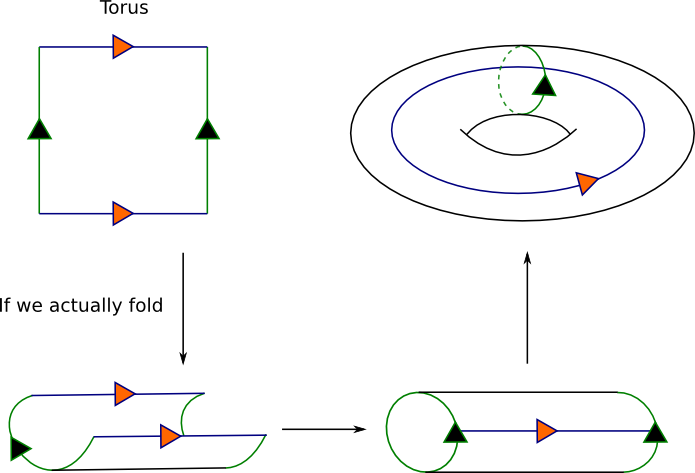
\includegraphics[width=\textwidth]{figures/part1.png}
            \captionof{figure}{Entstehung des Torus als Quotientenraum von $[0,1]^2$. \\
\tiny Quelle: \href{http://3.bp.blogspot.com/_swn7VcF-Vqc/TCpcMmi8qII/AAAAAAAAAHw/3QtMkZsikpY/s1600/part1(6).png}{http://3.bp.blogspot.com/\_swn7VcF-Vqc/TCpcMmi8qII/AAAAAAAAAHw/3QtMkZsikpY/s1600/part1(6).png}}
            \end{minipage} \\ \\
        \item Sei $X = [0,1] ^2 \subset \R^2$. Identifizieren wir $(t,0) \sim  (t,1)$ sowie $(0,s) \sim  (1, 1-s)$, so erhalten wir die \vocab{Kleinsche Flasche}. 
            \begin{minipage}{\textwidth}
                \begin{minipage}{0.3\textwidth}
                        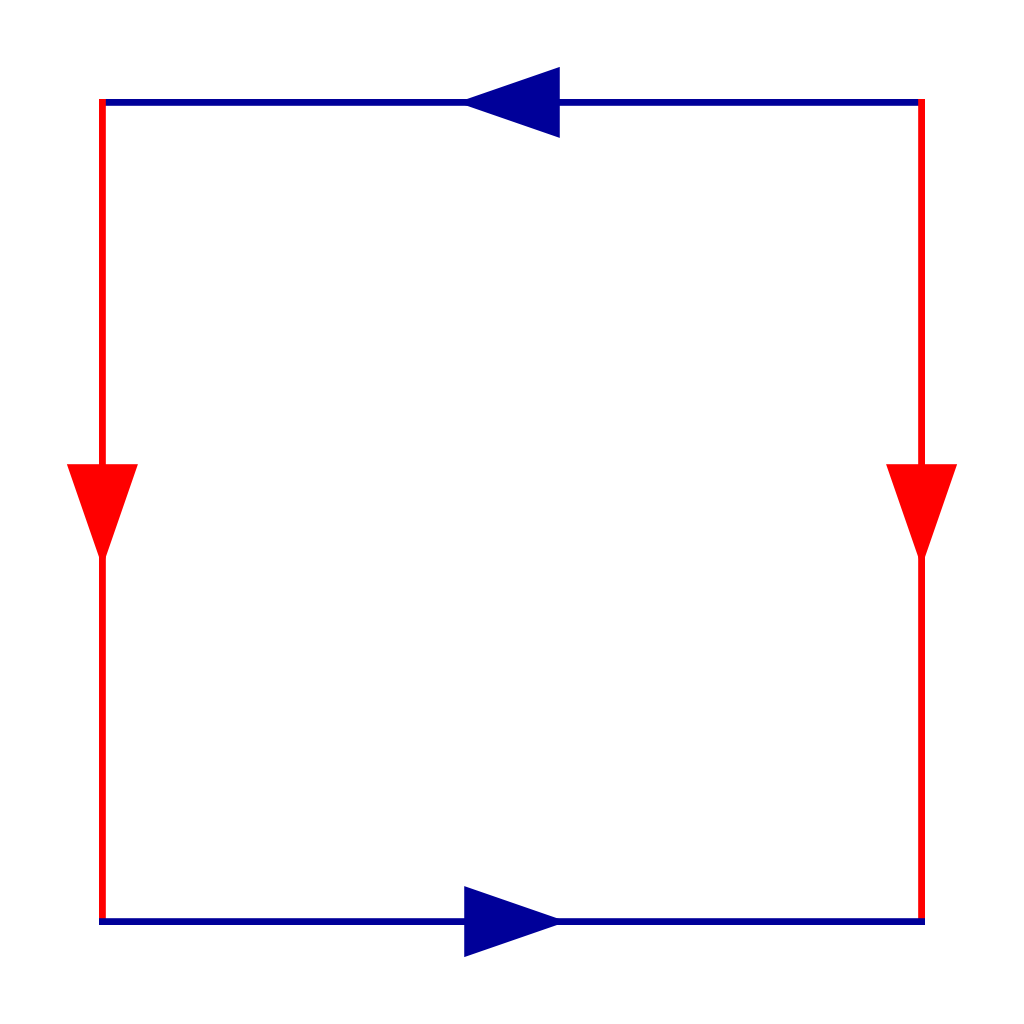
\includegraphics[width=\textwidth]{figures/1024px-Klein_Bottle_Folding_1.svg.png}
                \end{minipage}
                \begin{minipage}{0.3\textwidth}
                    \centering
                    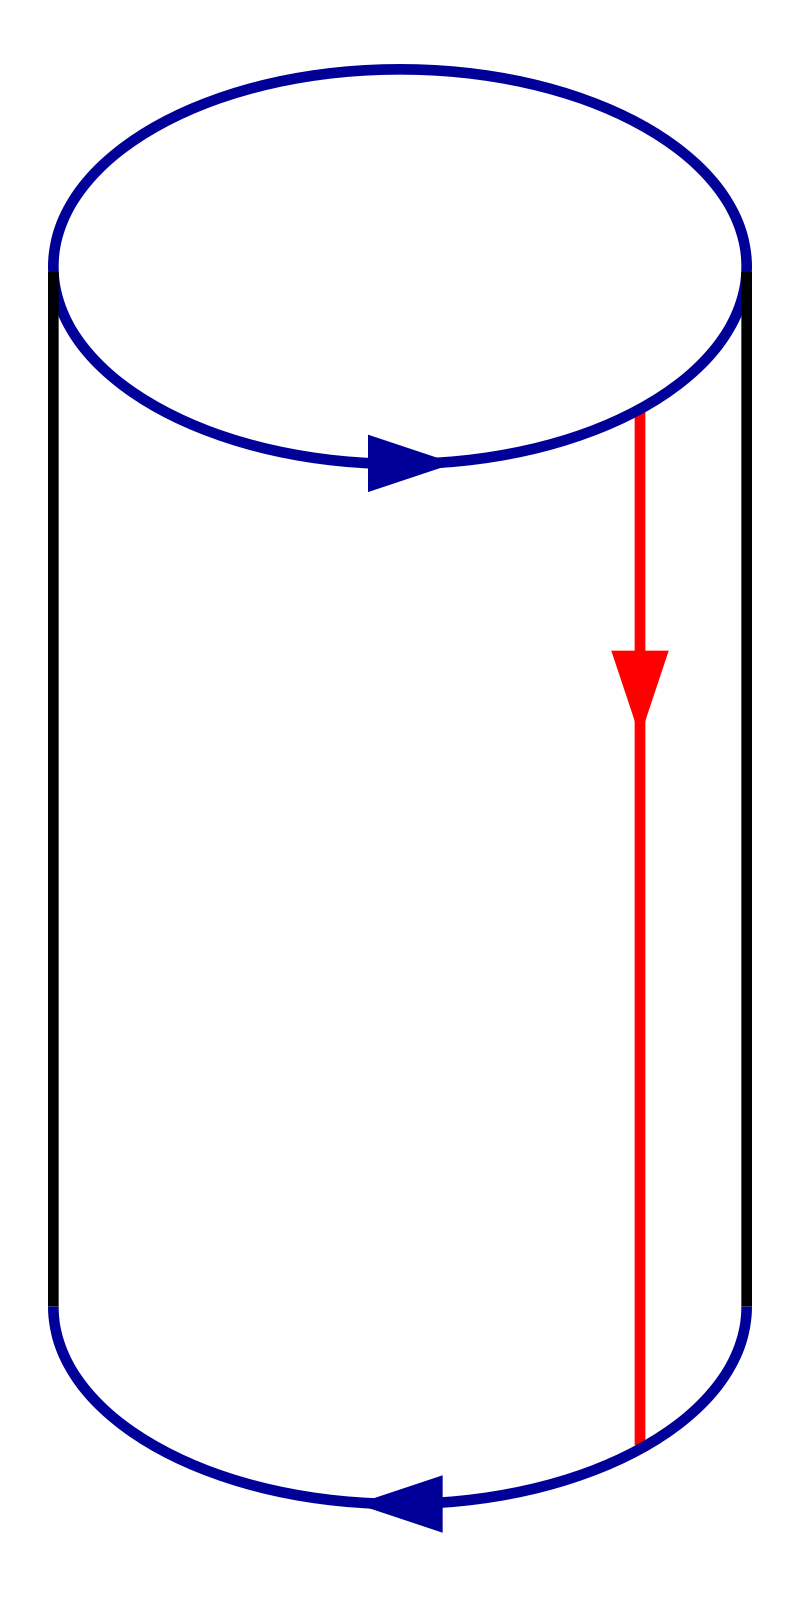
\includegraphics[width=0.6\textwidth]{figures/800px-Klein_Bottle_Folding_2.svg.png}
                \end{minipage}
                \begin{minipage}{0.3\textwidth}
                    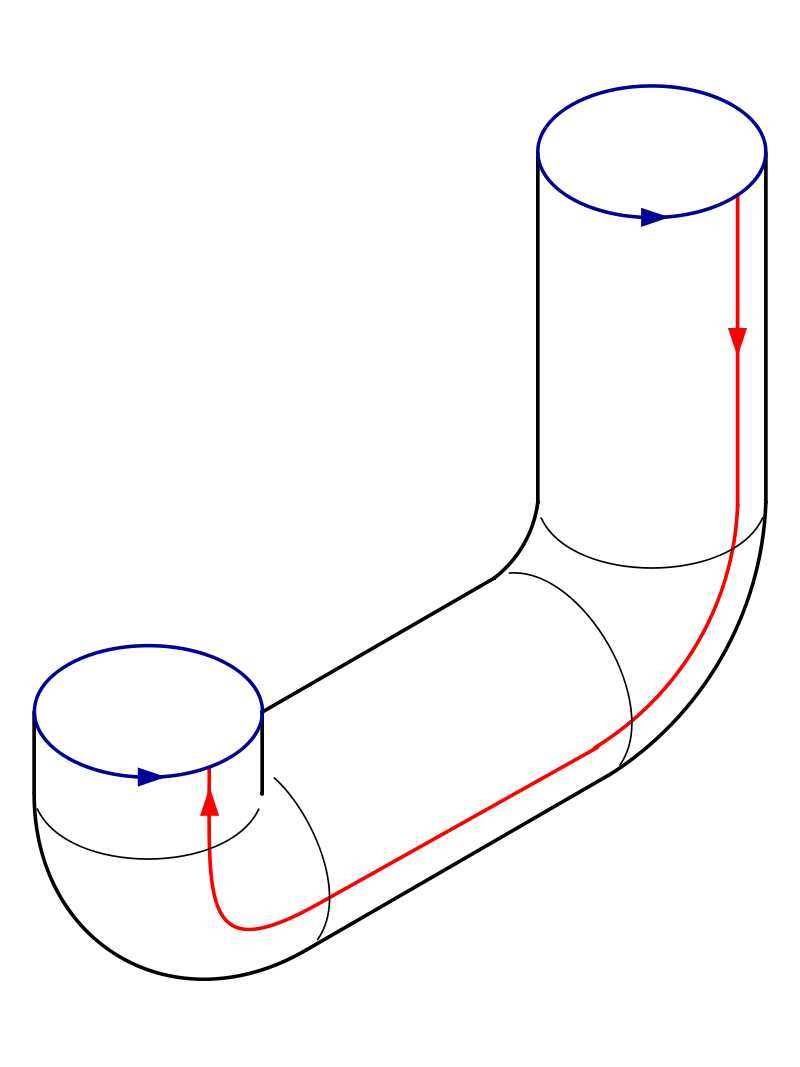
\includegraphics[width=\textwidth]{figures/800px-Klein_Bottle_Folding_3.svg.png}
                \end{minipage}
                \\
                \begin{minipage}{0.3\textwidth}
                    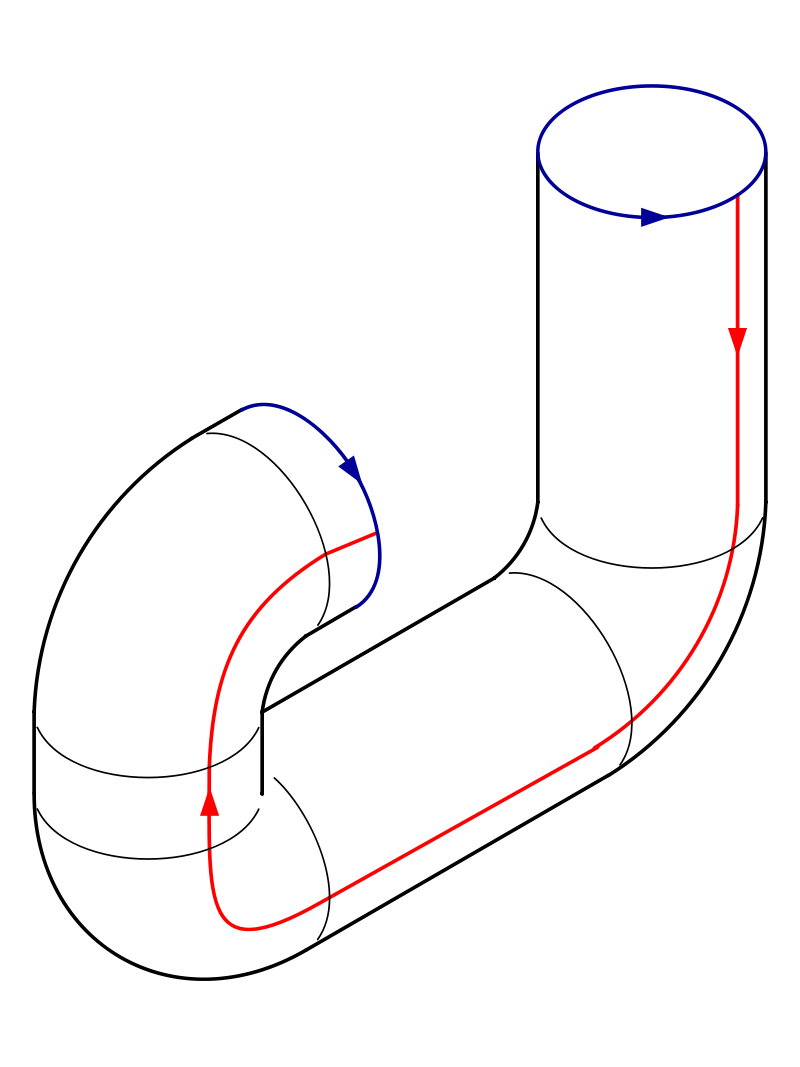
\includegraphics[width=\textwidth]{figures/800px-Klein_Bottle_Folding_4.svg.png}
                \end{minipage}
                \begin{minipage}{0.3\textwidth}
                    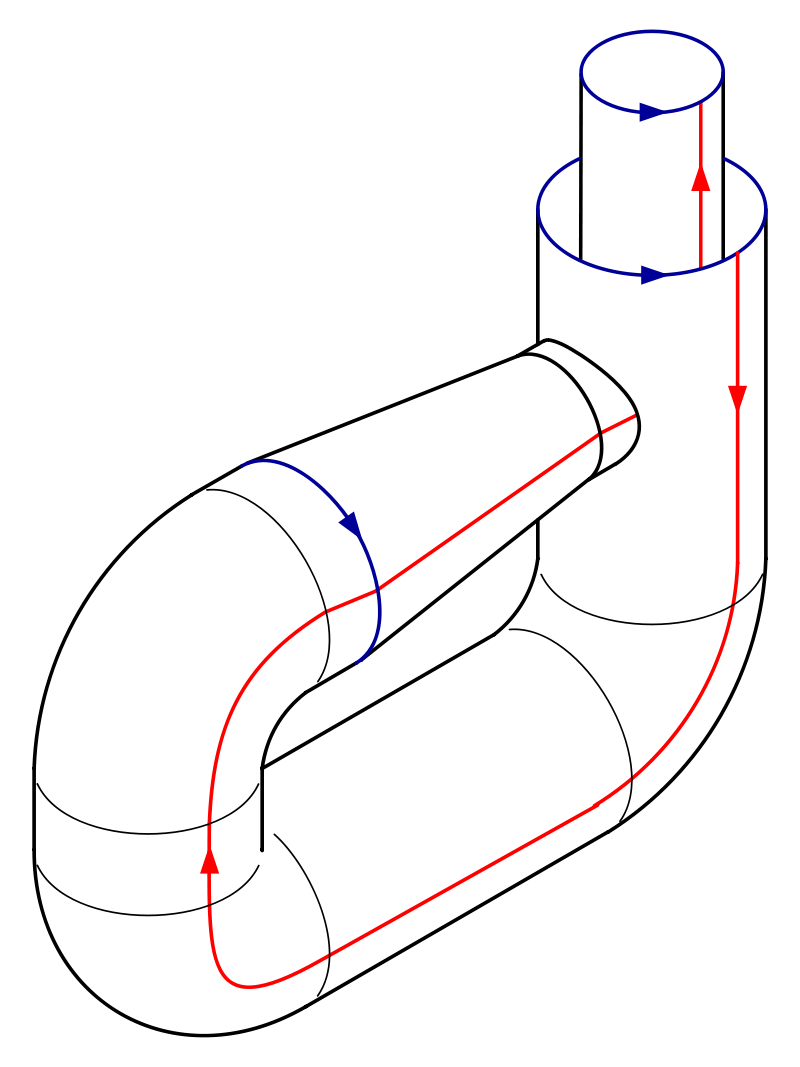
\includegraphics[width=\textwidth]{figures/800px-Klein_Bottle_Folding_5.svg.png}
                \end{minipage}
                \begin{minipage}{0.3\textwidth}
                    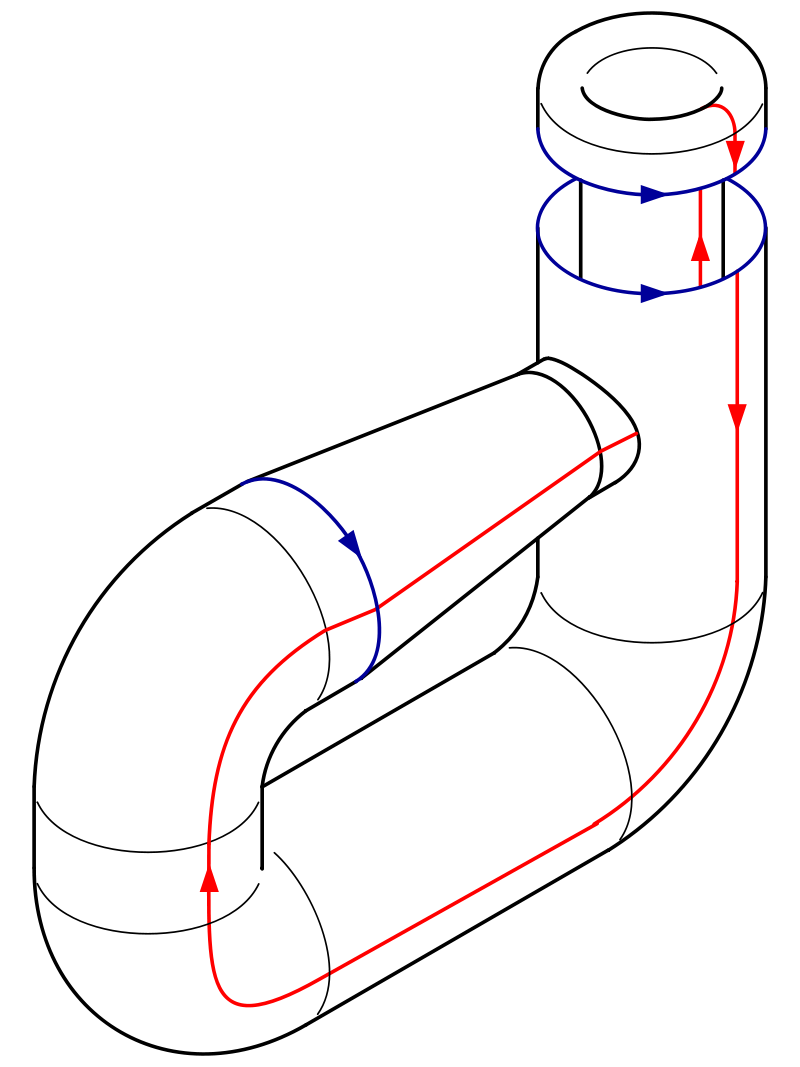
\includegraphics[width=\textwidth]{figures/800px-Klein_Bottle_Folding_6.svg.png}
                \end{minipage}
                \\
                \begin{minipage}{\textwidth}
                    \captionof{figure}{Entstehung der Kleinschen Flasche als Quotientenraum von $[0,1]^2$. \\ \tiny Quelle: \href{https://commons.wikimedia.org/wiki/File:Klein_Bottle_Folding_1.svg}{https://commons.wikimedia.org/wiki/File:Klein\_Bottle\_Folding\_1.svg}}
                \end{minipage}
            \end{minipage}
        \item Betrachte auf dem $\R^{n+1}\setminus \left \{0\right\} $ die Relation $x \sim  λx$ für $λ>0\in \R$. Dann ist $\R^{n+1} / \sim  \cong S^n$. Zunächst ist nämlich die Abbildung
                \begin{equation*}
                f: \left| \begin{array}{c c l} 
                \R^{n+1}\setminus \left \{0\right\}  & \longrightarrow & S^n \\
                x & \longmapsto &  \frac{x}{\lVert x \rVert _2}
                \end{array} \right.
            \end{equation*}
            stetig und die induzierte Abbildung $\R^{n+1} \setminus \left \{0\right\}  / \sim \to  S^n$ ist bijektiv. Das rechnen wir nach: Seien $x\neq y$ mit $d(x,y) < \delta$, so ist:
            \begin{equation}
                \begin{split}
                    d\left( \frac{x}{\lVert x \rVert },\frac{y}{\lVert y \rVert } \right) &\leq d\left( \frac{x}{\lVert x \rVert },\frac{y}{\lVert x \rVert } \right) + d\left( \frac{y}{\lVert x \rVert },\frac{y}{\lVert y \rVert } \right)  \\
                                                                                          &= \frac{1}{\lVert x \rVert } d(x,y) + \sqrt{\sum \left( \frac{y_i}{\lVert x \rVert }-\frac{y_i}{\lVert y \rVert } \right)^2 }  \\
                                                                                          &= \frac{1}{\lVert x \rVert } d(x,y) + \sqrt{\frac{(\lVert x \rVert -\lVert y \rVert )^2}{\lVert x \rVert \lVert y \rVert }} \lVert y \rVert \\
                                                                                          &< \frac{1}{\lVert x \rVert }\cdot \delta + \frac{\delta}{\lVert x \rVert ^2 + \delta \lVert x \rVert }(\lVert x \rVert +\delta) \to  0
                \end{split}
            \end{equation}
            also ist $f$ stetig. Mit der Inklusion  $ι: S^n \to  \R^{n+1} \setminus \left \{0\right\} $ erhalten wir
            \[
            f \circ  ι = \id_{S^n}
            .\] 
            Übung: Daraus folgt bereits, dass $S^n$ die Quotiententopologie trägt.
        \item Setzen wir erneut $X = \R^{n+1} \setminus \left \{0\right\} $, aber diesmal $x \sim  \lambda x$ für $λ\in \R \setminus  \left \{0\right\} $, so heißt der Quotient
            \[
            X / \sim  =: \R P^n
            .\] 
            der \vocab[Raum!reell projektiv]{reelle projektive Raum}.  Es ist
            \[
                \R P^n \cong S^n / (x \sim -x)
            .\] 
            Dies sehen wir mittels folgendem Diagramm:
            \begin{equation}
            \begin{tikzcd}
                \R^{n+1} \setminus \left \{0\right\}  \ar[two heads]{d} \ar[shift left]{r}{f} & S^n \ar[shift left]{l}{ι} \ar[two heads]{d} \\
                \R P^n \ar[dashed, shift left]{r}{\overline{f}} & S^n / (x \sim  - x) \ar[dashed, shift left]{l}{\overline{ι}}
            \end{tikzcd}
            \end{equation}
            Die Abbildungen $\overline{ι}$ und $\overline{f}$ sind stetig nach der universellen Eigenschaft und invers zueinander. \\
            \begin{minipage}{\textwidth}
                \centering
\begin{tikzpicture}
    \draw[->] (-1.5,0) -- (1.5,0);
    \draw [->] (0,-1.5) -- (0,1.5);
    \draw (1,0) arc (0:90:1);
    \draw[red] (0,0) -- (1.5,1);
    \draw[red] (0,0) -- (1.5,1.3);
    \draw[red] (0,0) -- (1,1.5);
    \draw[blue] (-1.5,-1.5) -- (1.5,1.5);
\end{tikzpicture}
\captionof{figure}{Konstruktion des reellen projektiven Raums für den Fall $n=1$. Wir identifizieren die roten Strahlen miteinander, nicht jedoch den gesamten blauen, da $λ>0$.}
            \end{minipage}
            \\ 
        \item Sei $X$ ein topologischer Raum und  $A\subset X$ eine Teilmenge. Definiere die Relation $\sim $ durch $a\sim a'$ für $a,a'\in A$ (bzw. erzeuge eine dadurch). Dann setzen wir
            \[
            X / A := X / \sim 
            .\] 
            Es ergibt sich
            \begin{itemize}
                \item $[0,1] / \left \{0,1\right\} \cong S^1$ 
                \item $[0,1] / [0,1)$ hat zwei Punkte  $[0,1)$ und  $\left \{1\right\} $. Es ist $[0,1) \subset [0,1]$ offen, aber $\left \{1\right\} $ nicht, also handelt es sich um den Sierpinski-Raum.
            \end{itemize}
    \end{enumerate}
\end{example}
\begin{remark}
    Quotientenräume von metrischen Räumen sind im Allgemeinen nicht metrisierbar.
\end{remark}




\section{Trennungsaxiome}
\begin{definition}[Hausdorff'sch]\label{def:hausdorff}
    Ein topologischer Raum heißt \vocab[Topologischer Raum!Hausdorff]{Hausdorff} (oder \vocab[Topologischer Raum!Hausdorff'sch]{Hausdorffsch}), wenn $\forall x,y\in X$ mit $x\neq y$ offene Mengen $U_x, U_y\subset X$ existieren mit $x\in U_x$ und $y\in U_y$, sodass $U_x \cap U_y = \emptyset$. Diese Eigenschaft heißt auch Trennungsaxiom\index{Trennungsaxiom} \vocab[Trennungsaxiom!$T_2$]{$T_2$}. \\
    \begin{minipage}{\textwidth}
    \centering    
\begin{minipage}{0.3\textwidth}
        \centering
        \incfig{hausdroff-raum}
    \end{minipage}
    \end{minipage}
\end{definition}

\begin{theorem}\label{thm:metrisierbarer-raum-ist-hausdorff}
    Ist $X$ metrisierbar, so ist  $X$ Hausdorffsch.
\end{theorem}
\begin{proof}
    Sei $d$ eine Metrik auf  $X$, die die Topologie induziert. Seien  $x,y\in X$ mit $x\neq y$. Setze
    \[
        U_x := U\left( x, \frac{d(x,y)}{2} \right) \qquad U_y = U\left( y, \frac{d(x,y)}{2} \right) 
    .\] 
    Dann ist $U_x \cap U_y = \emptyset$, denn für alle $z\in U_x \cap U_y$ ist
    \[
        d(x,y) \leq  d(x,z) + d(z,y) < \frac{d(x,y)}{2} + \frac{d(x,y)}{2} = d(x,y)
    .\] 
    , was nicht sein kann.
\end{proof}
\begin{example}
    $\R^n$ ist Hausdorffsch.
\end{example}
\begin{theorem}\label{thm:hausdorff-impliziert-t1}
    Ist $X$ Hausdorffsch und  $x\in X$, dann ist $\left \{x\right\} \subset X$ abgeschlossen.
\end{theorem}
\begin{proof}
    Für $y\neq x$ existiert $U_y$ offen mit  $x\not\in U_y$ und $y\in U_y$. Dann ist
    \[
    X \setminus \left \{x\right\}  = \bigcup_{y\neq x} U_y 
    .\] 
    offen. \\
\end{proof}
    \begin{minipage}{\textwidth}
        \centering
    \incfig{hausdorff-impliziert-t1}
    \captionof{figure}{Skizze zum Beweis von \autoref{thm:hausdorff-impliziert-t1}}
    \end{minipage}
\begin{remark}
    Ein topologischer Raum, für den alle $\left \{x\right\} $ abgeschlossen sind, heißt \vocab[Trennungsaxiom!$T_1$]{$T_1$-Raum}.
\end{remark}
\begin{remark*}
    Man findet in der Literatur auch folgende Definition: \\
    Ein topologischer Raum heißt $T_1$-Raum, wenn es für je zwei verschieden Punkte $x\neq y$ Umgebungen $U_x,U_y$ gibt mit  $x\in U_x, y\in U_y$ und $x\not\in U_y, y\not\in U_x$. \\
    Im Gegensatz zum Hausdorff-Raum trennen wir zwei Punkte also durch 2 nicht notwendigerweies offene Umgebungen. Mit dem gleichen Beweis wie in \autoref{thm:hausdorff-impliziert-t1} zeigen wir dann, dass jeder Punkt abgeschlossen ist. Ist umgekehrt $X$ ein Raum, in dem alle Punkte abgeschlossen sind, so können wir  $x,y$ stets durch die offenen Umgebungen  $y\in X \setminus \left \{x\right\} $ sowie $x\in X \setminus \left \{y\right\} $ trennen. Die beiden Definitionen sind also äquivalent.
    \begin{minipage}{\textwidth}
    \incfig{t1-raum}
    \captionof{figure}{Ein $T_1$-Raum}
    \end{minipage}
\end{remark*}



\begin{lemma}\label{lm:teilraum-von-hausdorffraum-ist-hausdorff}
    Sei $X$ Hausdorffsch und $A\subset X$ ein Teilraum. Dann ist auch $A$ Hausdorffsch.
\end{lemma}
\begin{proof}
    Sei $x\neq y\in A$. Dann existieren $U_x, U_y\subset X$ offen mit $x\in U_x$ und $y\in U_y$ sowie $U_x \cap U_y = \emptyset$. Dann sind
    \[
    U_x \cap A \qquad U_y \cap A \subset A
    .\] 
    offen in $A$ und erfüllen die Bedingungen.
\end{proof}


\begin{remark}
    Jeder diskrete Raum ist Hausdorffsch. Ist $X$ endlich und Hausdorffsch, so ist  $X$ diskret.
\end{remark}
\begin{proof}
    Für jedes $y\neq x$ existiert ein $U_x^y$ offen mit  $x\in U_x^y$ und $y\not\in U_x^y$. Dann ist aber
    \[
    \left \{x\right\}  = \bigcap_{y\neq x} U_x^{y}
    .\] 
    offen (da $X$ endlich), also ist $X$ diskret. Die Umkehrung ist offensichtlich.
\end{proof}
\begin{example}
    $S^n \subset \R^{n+1}$ ist Hausdorffsch.
\end{example}

\begin{definition}[Normal]\label{def:normal}
    Ein topologischer Raum heißt \vocab[Topologischer Raum!normal]{normal}, falls
    \begin{itemize}
        \item $X$ ist Hausdorffsch
        \item  $\forall A,B\subset X$ abgeschlossen mit $A \cap B = \emptyset$ existieren $U_A, U_B \subset X$ offen mit $A\subset U_A$, $B\subset U_B$ und $U_A \cap U_B = \emptyset$. Diese Eigenschaft heißt auch Trennungsaxiom \vocab[Trennungsaxiom!$T_4$]{$T_4$}. \\
            \begin{minipage}{\textwidth}
                \centering
                \begin{minipage}{0.3\textwidth}
    \incfig{normaler-raum}
                \end{minipage}
            \end{minipage}
    \end{itemize}
\end{definition}


\begin{remark}
    Manchmal gibt es diese Definition auch ohne Hausdorff'sch.
\end{remark}

\begin{theorem}\label{thm:metrischer-raum-ist-normal}
    Ist $X$ metrisierbar, dann ist  $X$ normal.
\end{theorem}

\begin{proof}
    Übung.
\end{proof}

\begin{definition}[Regulär]\label{def:regulär}
    Ein topologischer Raum $X$ heißt  \vocab[Topologischer Raum!regulär]{regulär}, falls $X$ Hausdorff ist und  $\forall  A \subset X$ abgeschlossen und $x\in X \setminus A$ existieren $U_a, U_{x}$ offen mit $A\subset U_A, x\in U_x$ und $U_A \cap U_x = \emptyset$. (Auch Trennungsaxiom \vocab[Trennungsaxiom!$T_3$]{$T_3$} genannt). \\
    \begin{minipage}{\textwidth}
        \centering
        \begin{minipage}{0.7\textwidth}
        \centering
        \incfig{regular-space}
        \end{minipage}
    \end{minipage}
\end{definition}

\begin{remark}
    Klarerweise gilt $T_4 \implies T_3$, d.h. jeder normale Raum ist auch regulär. Hierzu benötigen wir nur, dass Punkte in $T_4$-Räumen abgeschlossen sind, aber das folgt mit \autoref{thm:hausdorff-impliziert-t1}, bzw. damit, dass wir bereits $T_4 \implies T_2 \implies T_1$ wissen.
\end{remark}
\begin{figure}[ht]
    \centering
    \label{fig:regular-space}
\end{figure}


\section{Kompaktheit}
Aus der Analysis ist (vielleicht) folgender Satz bekannt.
\begin{theorem}[Heine-Borel]\label{thm:heine-borel}
    Für $X\subset \R^n$ sind äquivalent:
    \begin{enumerate}[1)]
        \item $X$ ist abgeschlossen und beschränkt.
        \item Jede offene Überdeckung von $X$ hat eine endliche Teilüberdeckung
    \end{enumerate}
\end{theorem}

\begin{recap}
    'Jede offene Überdeckung besitzt eine endliche Teilüberdeckung' bedeutet: \\
    Für jede Familie $\left \{U_i\right\} _{i \in I}$ mit $U_i \subset X$ offen und $X \subset \bigcup_{i \in I}U_i$ existiert eine endliche Teilmenge $J\subset I$ mit $X \subset \bigcup_{j\in J} U_j$
\end{recap}
\begin{proof}
    später.
\end{proof}

\begin{definition}[Kompaktheit]\label{def:kompakt}
    Ein topologischer Raum $X$ heißt  \vocab[Topologischer Raum!kompakt]{kompakt}, falls jede offene Überdeckung eine endliche Teilüberdeckung besitzt.
\end{definition}
\begin{remark}
    Manchmal heißt obige Definition auch quasi-kompakt, und kompakt bedeutet dann quasi-kompakt + Hausdorff.
\end{remark}

\begin{example}
   Die Räume
   \[
       [0,1] \subset \R \qquad S^n \subset \R^{n+1}
   .\] 
   sind beide kompakt (nach \ref{thm:heine-borel})
\end{example}

    \lecture{4}{Do 22 Apr 2021 10:15}{}
\begin{example}
    Zur Frage von letzter Woche (wenn wir einen Hausdorff-Raum haben und eine Äquivalenzrelation, deren Klassen abgeschlossen sind, ist dann der Quotient wieder  Hausdorff?): Wähle auf $[0,1]$ die Relation erzeugt von
     \[
    \frac{1}{n} \sim  1 - \frac{1}{n}
    .\] 
    für alle $n\in \N_>0$. Betrachte dann die Abbildung: 
    \[
        [0,1] \twoheadrightarrow [0,1] / \sim 
    .\] 
    Punkturbilder sind endlich, also abgeschlossen. Aber der Raum $[0,1] / \sim $ ist nicht hausdorffsch, denn wri können die Punkte $0,1$ nicht trennen.
\end{example}
\begin{theorem}
    Sei $X$ ein kompakter Raum und  $Y\subset X$ abgeschlossen. Dann ist $Y$ kompakt.
    \label{thm:closed-subset-of-compact-space-is-compact}
\end{theorem}
\begin{proof}
    Sei $\left \{U_i\right\} _{i \in I}$ eine offene Überdeckung von $Y$. Dann existieren $U_i' \subset X$ offen mit $U_i = U_i' \cap Y$. Die Familie
     \[
    \left \{U_i'\right\} _{i \in I}\cup \left \{\underbrace{X \setminus Y}_{\text{offen}}\right\} 
    .\] 
    ist nun eine offene Überdeckung von $X$. Dann existiert $J\subset I$ endlich, so dass
    \[
    \left \{U_j'\right\} _{j\in J} \cup \left \{X \setminus Y\right\} 
    .\] 
    die Menge $X$ überdeckt. Also ist  
    \[
        \left \{\underbrace{U_j' \cap Y}_{U_j}\right\} _{j\in J} \cup \left \{\underbrace{X \setminus Y \cap Y}_{=\emptyset}\right\}  
    \]
    eine endliche Überdeckung für $Y$.
\end{proof}
\begin{theorem}
    Sei $X$ ein Hausdorff-Raum und  $Y\subset X$ kompakt. Dann ist $Y$ abgeschlossen.
    \label{thm:compact-subset-of-hausdorff-space-is-closed}
\end{theorem}

\begin{corollary}
    Ist $X$ kompakt und Hausdorffsch, dann sind äquivalent:
    \label{thm:compact-iff-closed}
\begin{enumerate}[1)]
        \item $Y\subset X$ ist abgeschlossen
        \item $Y$ ist kompakt.
    \end{enumerate}
\end{corollary}
\begin{lemma}
    Sei $X$ ein Hausdorff Raum und  $Y\subset X$ kompakt. Dann existiert $\forall x\in X\setminus Y$ offene Teilmengen $U_{x,Y}$ und $V_{x,Y}$ von $X$ so dass:  $x\in U_{x,Y}$ und $Y\subset V_{x,Y}$ und $U_{x,Y} \cap V_{x,Y} = \emptyset$.
    \label{lm:compact-set-in-hausdorff-space-is-closed}
\end{lemma}
\begin{proof}
    Sei $x\in X\setminus Y$. $\forall y\in Y$ existieren $U_{x,y}$ und $V_{x,y}$ offen mit $x\in U_{x,y}$ und $y\in V_{x,y}$, weil $X$ Hausdorffsch. \\
    Dann ist  $\left \{V_{x,y} \cap Y\right\} _{y\in Y}$ eine offene Überdeckung von $Y$. Also existiert endliche Teilüberdeckung (da  $Y$ kompakt) induziert durch Punkte  $y_1,\ldots,y_n$. Also:
    \[
    Y\subset \bigcup_{i=1}^n V_{x,y_i}
    .\] 
    Sei
    \[
    V_{x,Y} := \bigcup_{i=1}^n V_{x,y_i} \qquad U_{x,Y} := \bigcap_{i=1}^n U_{x,y_i} 
    .\] 
    Es ist auch $x\in U_{x,Y}$, weil $x\in U_{x,y_i}$ für jedes $i$. Wir müssen also noch Disjunktheit prüfen, es ist:
     \[
    U_{x,Y} \cap V_{x,y_i} \subset U_{x,y_i} \cap V_{x,y_i} = \emptyset
    .\] 
    Also auch
    \[
        \emptyset=    U_{x,Y} \cap \bigcup_{i=1}^n V_{x,y_i} = U_{x,Y} \cap V_{x,Y}
    .\]
\end{proof}
    \begin{figure}[H]
    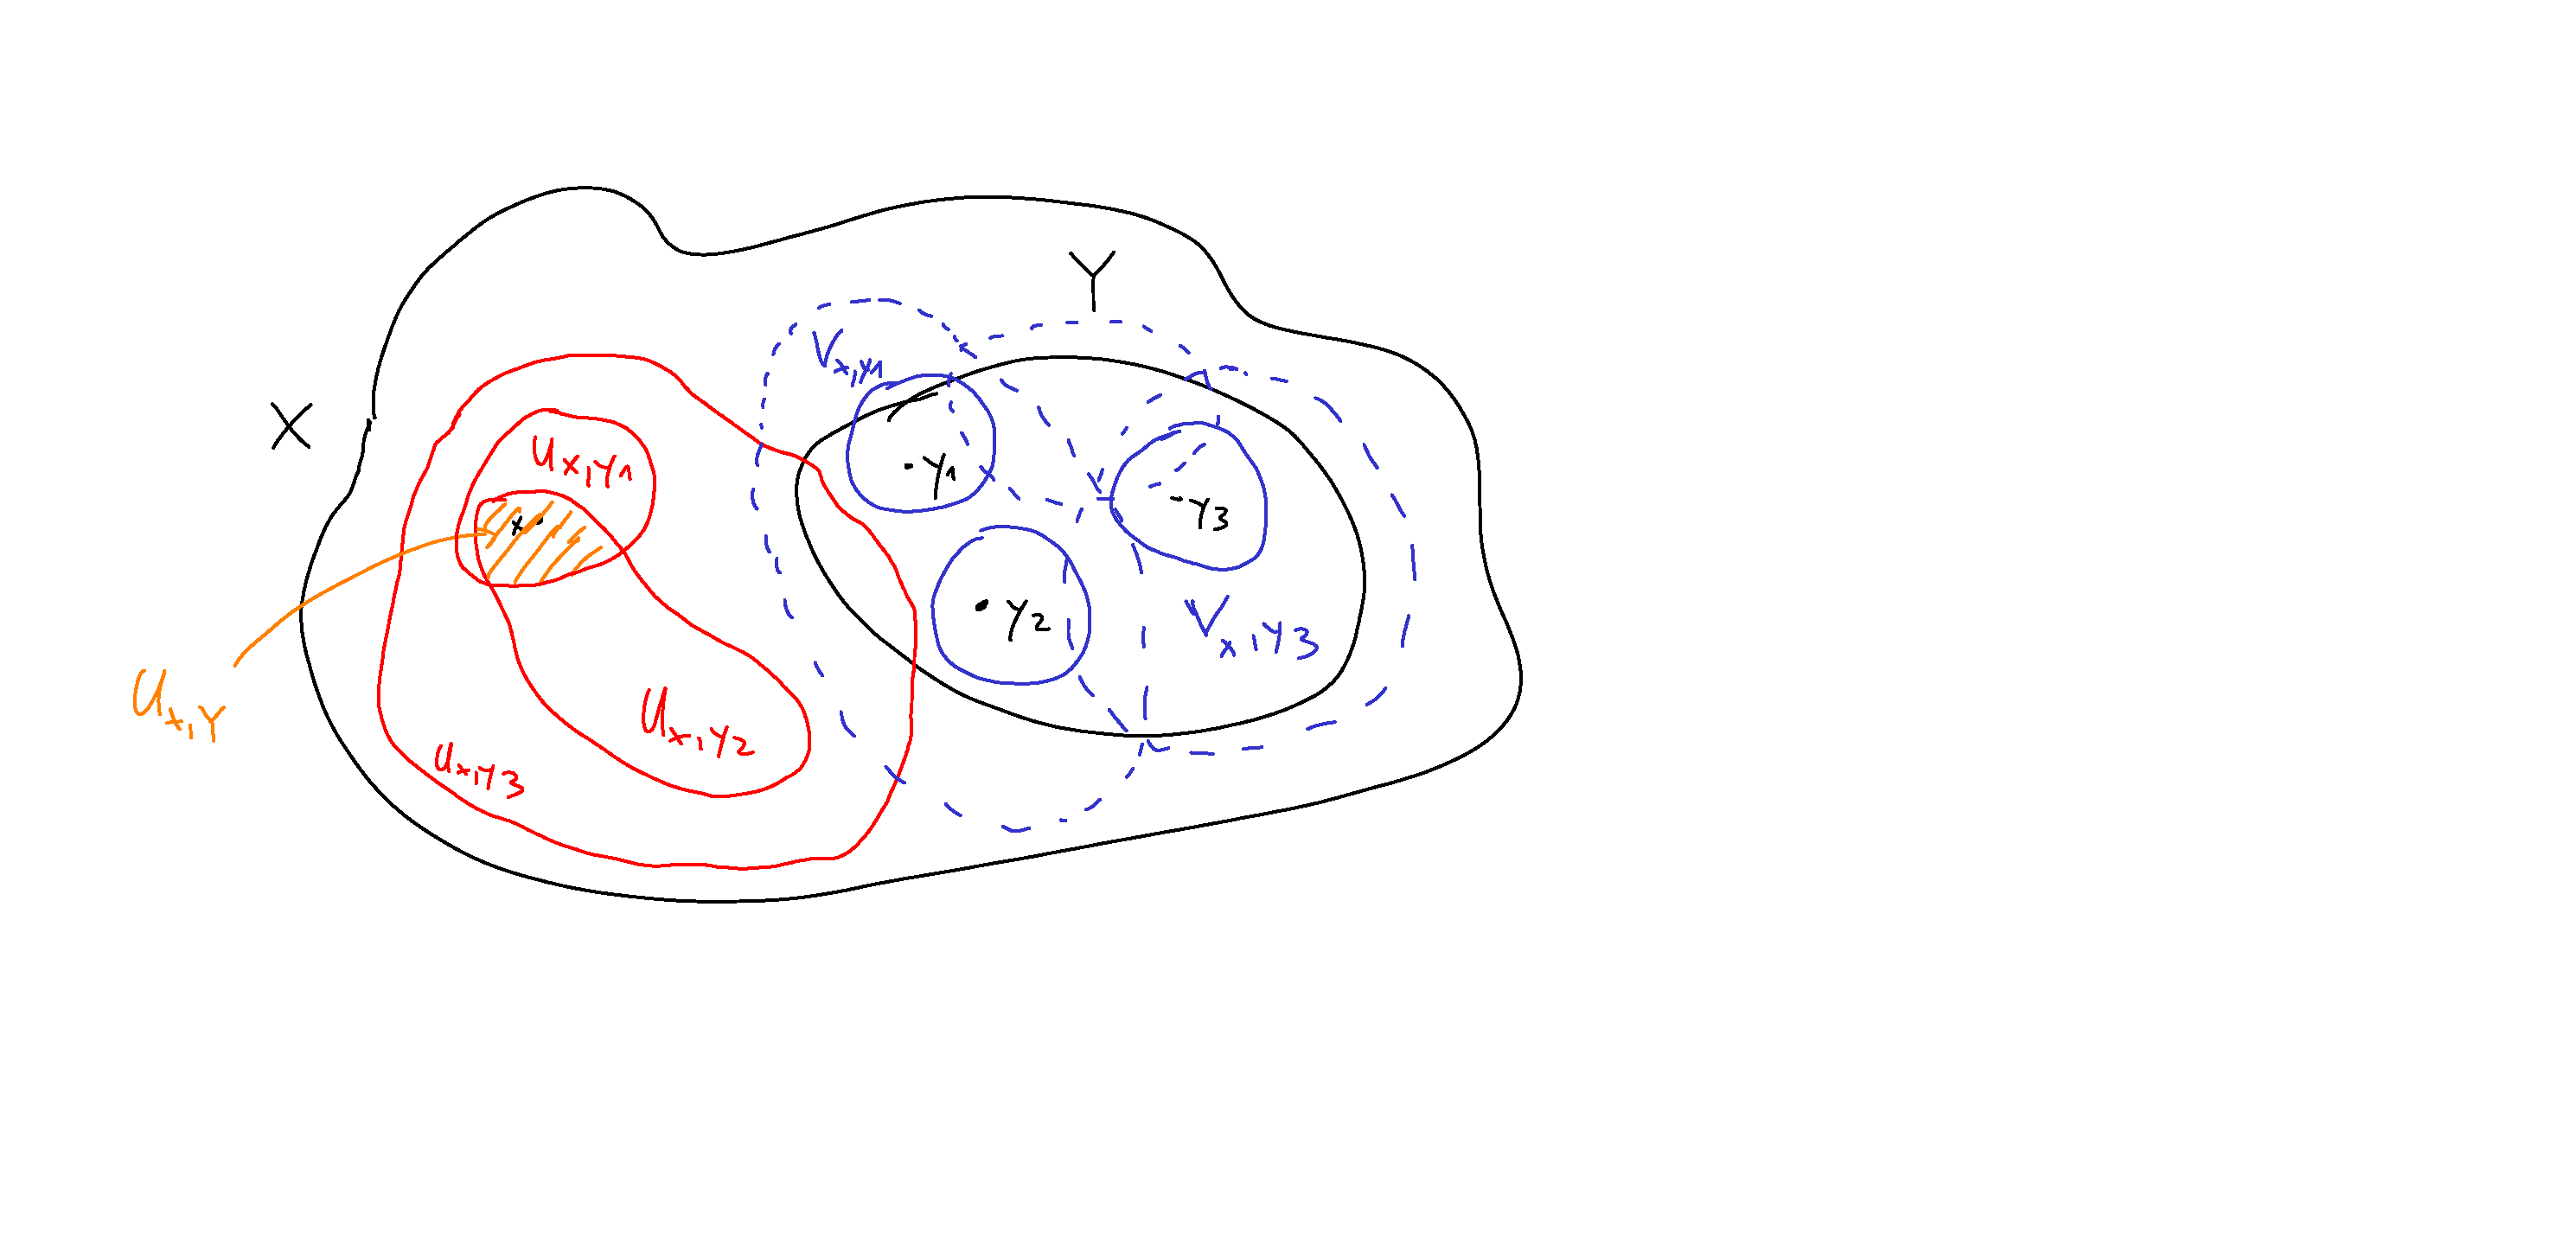
\includegraphics[scale=0.4]{figures/Lemma5.5.pdf}
    \caption{Skizze zum Beweis von Lemma \ref{lm:compact-set-in-hausdorff-space-is-closed}}
\end{figure}
\begin{proof}[Beweis von \ref{thm:compact-subset-of-hausdorff-space-is-closed}]
    Nach dem Lemma existieren $\forall x\in X \setminus Y$ ein $U_{x,Y}$ mit $x\in U_{x,Y}$ und $U_{x,Y} \cap Y = \emptyset$. Also ist
    \[
    X \setminus Y = \bigcup_{x\in X \setminus Y} U_{x,Y}
    .\] 
    offen und somit ist $Y$ abgeschlossen.
\end{proof}


\begin{example}['Gegenbeispiel' zu Satz \ref{thm:compact-subset-of-hausdorff-space-is-closed}]
    Sei $G$ die Gerade mit zwei Urpsrüngen: \\
    Betrachte  $\R\cup \left \{0'\right\} $ mit $U$ Umgebung von  $a\in \R$ falls $\exists ε>0$ mit $(a-ε, a+ε)\subset U$ und $U$ Umgebung von  $0'$ und  $U$ Umgebung von  $0'$, falls  $\exists ε>0$ mit $(-ε,0 \cup (0,ε) \subset U$ und $0' \in U$. \\
    Wir können uns gewissermaßen  $0,0'$ gleichberechtigt vorstellen, nur dass die beiden Punkte verschieden sind. \\
    Dann ist  $[-1,1] \subset G$ kompakt (Übung!), aber nicht abegschlossen, da $0' \in G \setminus [-1,1]$ ist, dies aber keine Umgebung von $0'$ ist.
    \begin{figure}[H]
        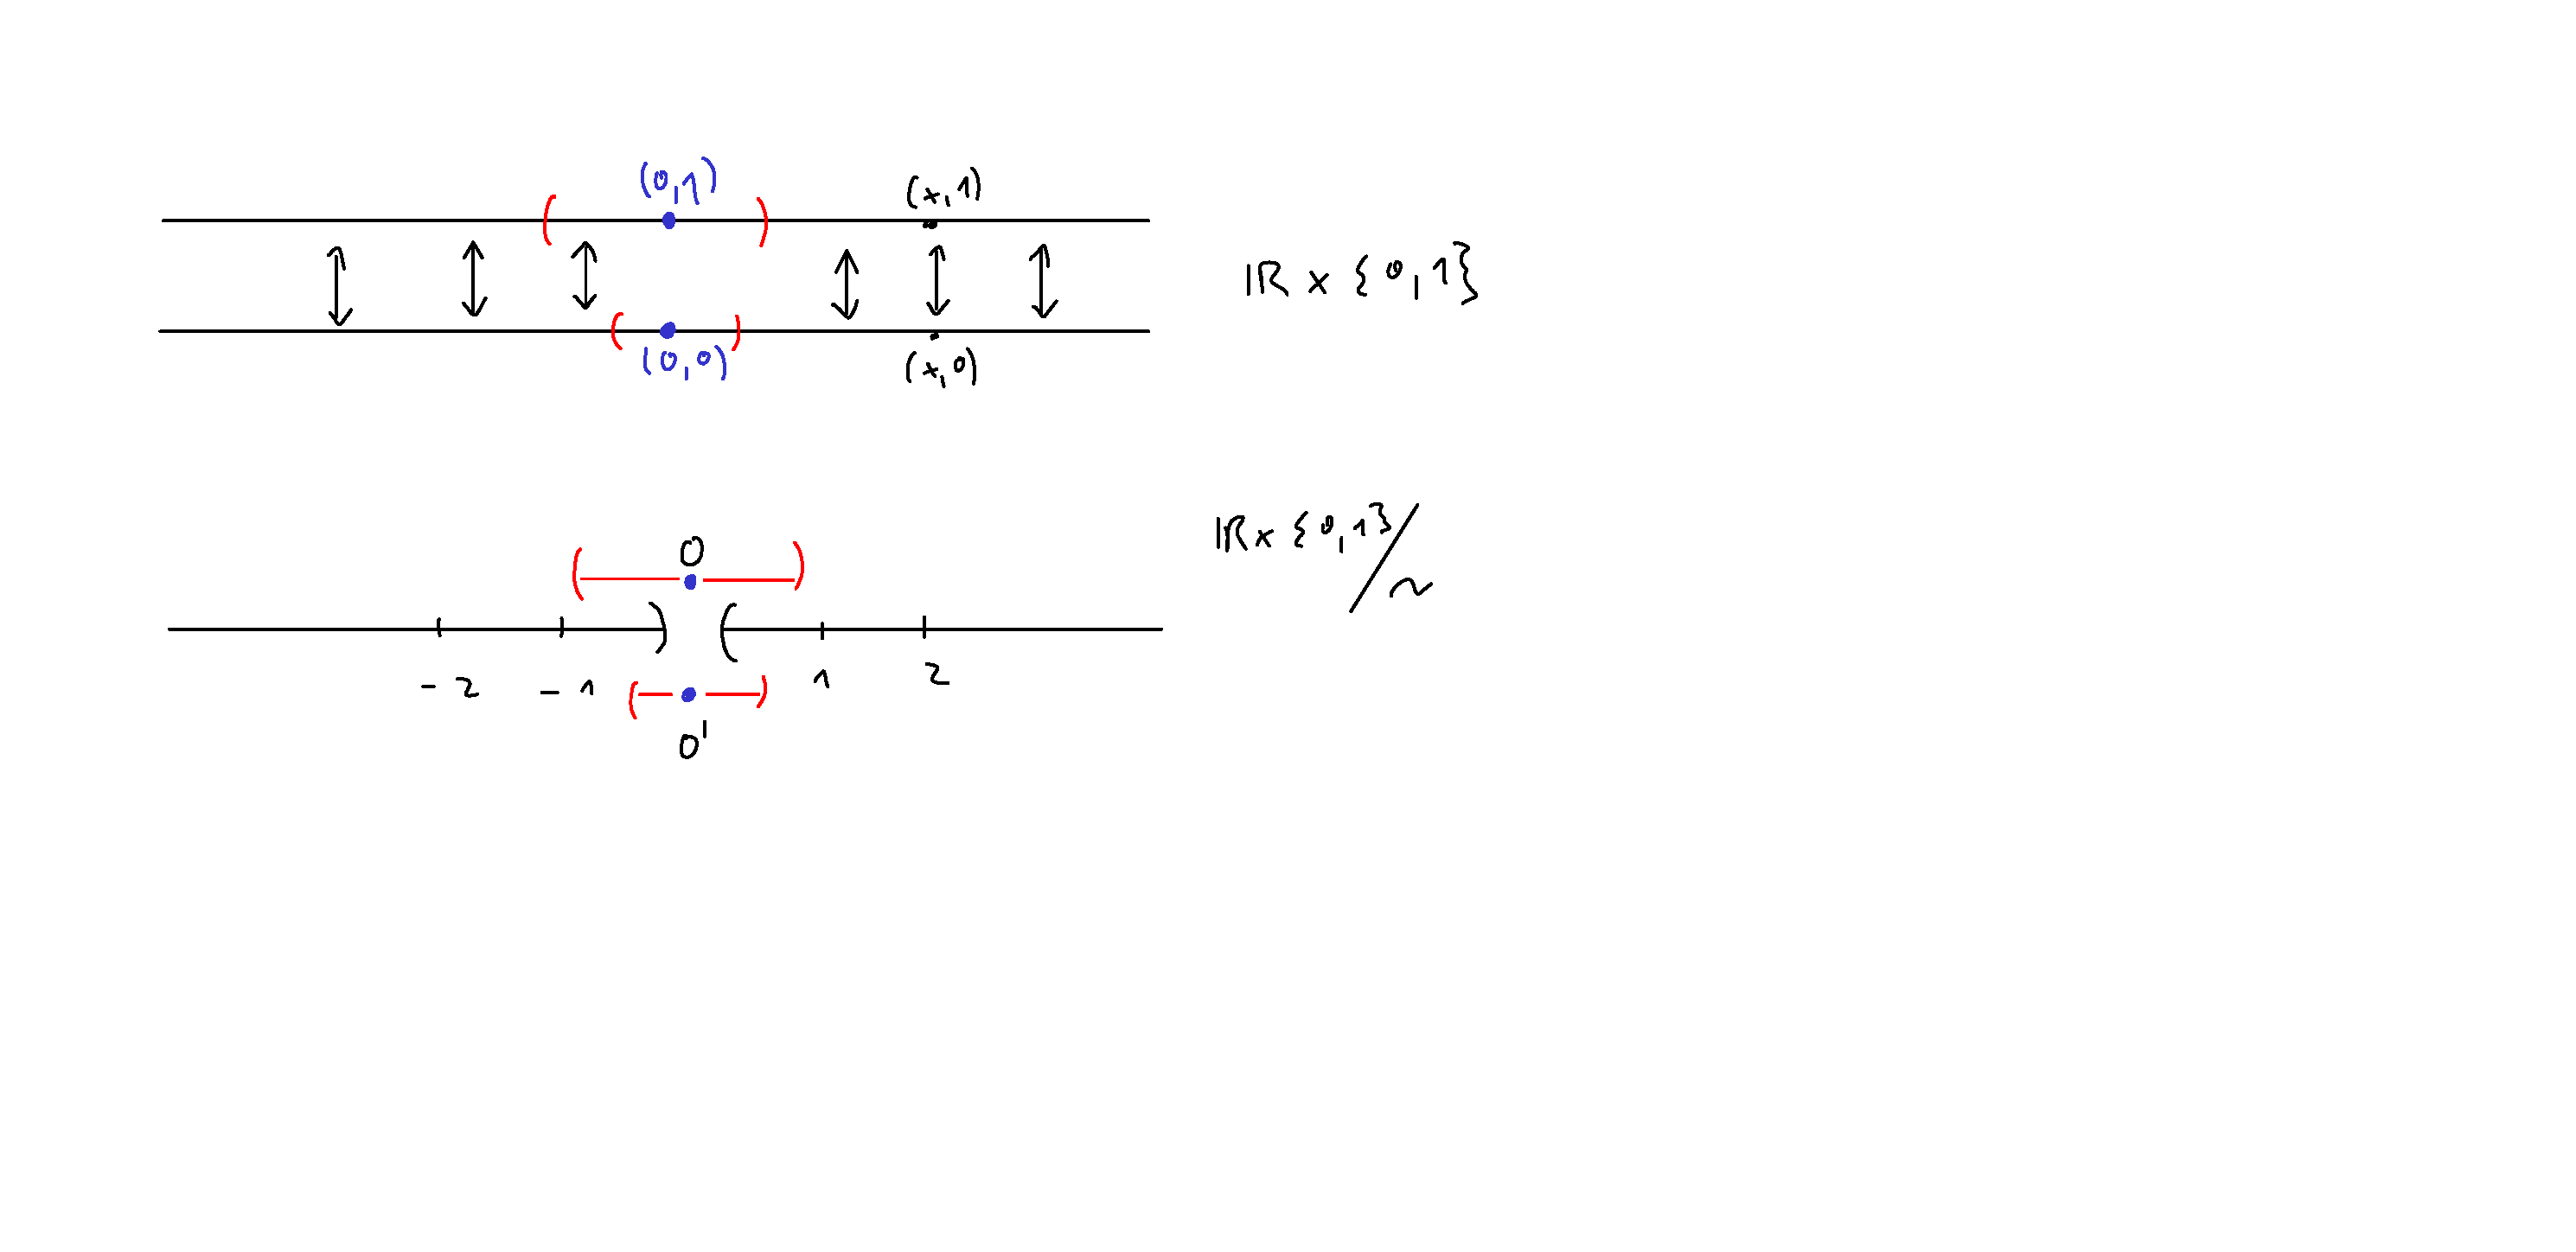
\includegraphics[scale=0.4]{figures/line-with-2-origins.pdf}
    \caption{Gerade mit 2 Ursprüngen}
    \end{figure}
\end{example}


\begin{proof}[Beweis von Satz \ref{thm:heine-borel}]
    '$2) \implies 1)$'. Sei $X\subset \R^n$ kompakt. Dann ist sie abgeschlossen nach \ref{thm:compact-subset-of-hausdorff-space-is-closed}. Zudem ist $X\subset \bigcup_{x\in X} U(x,1)$ eine offene Überdeckung. Da $X$ kompakt finden wir endlich viele  $x_1,\ldots,x_n\in X$ mit
    \[
        X \subset \bigcup_{i=1}^n U(x_i,1)
    .\] 
    Also ist
    \[
        \diam(X) \leq  \max \left \{d(x_i,x_j)\right\} +2 < \infty
    .\] 
    und somit ist $X$ auch beschränkt. \\
    ' $1)\implies 2)$'. Da $X$ beschränkt ist,  $\exists m>0$ mit $X\subset [-m,m]^n\subset \R^n$. Da $X$ abgeschlossen ist, genügt es nach \ref{thm:closed-subset-of-compact-space-is-compact} zu zeigen, dass  $[-m,m]^n$ kompakt ist. \\
    Wir führen einen Widerspruchsbeweis, nimm also an, dass  $[-m,m]^n$ nicht kompakt ist. Dann existiert eine offene Überdeckung  $\left \{U_i\right\} _{i \in I}$ ohne endliche Teilüberdeckung. \\
    Unterteile $[-m,m]^n$ in  $2^n$ gleich große Unterwürfel (halbiere jede Seite). Mindestens ein Unterwürfel hat keine endliche Teilüberdeckung. Unterteile diesen Würfel weiter und wähle wieder einen Unterwüfel, der keine endliche Teilüberdeckung hat. \\
    Wir erhalten eine Folge von Würfeln
     \[
         [-m,m]^n =     Q_0 \supset Q_1 \supset Q_2 \supset Q_3 \supset \ldots
    .\] 
    die jeweils keine endliche Teilüberdeckung durch $U_i's$ besitzen. \\
    Sei  $x_i \in Q_i$ beliebig. Dann ist $x_i$ eine Cauchy-Folge, also existiert $x = \lim_{i\to \infty} x_i$, und $x\in Q_0$, da $Q_0$ abgeschlossen. \\
    Somit gibt es ein $U_j$ mit  $x\in U_j$, da die $\left \{U_i\right\} _{i \in I}$ eine Überedeckung von $Q_0$ waren. Damit ist auch $U(x,ε) \subset U_j$ für ein $ε>0$. Wähle einen Würfel $x\in Q_k$ mit Kantenlänge $< \frac{ε}{\sqrt{n} }$, dann ist auch $Q_k \subset U(x,ε) \subset U_j$. Das ist aber ein Widerspruch dazu, dass $Q_k$ keine endliche Teilüberdeckung hat, \contra. \\
    Also ist  $Q_0$ kompakt.
\end{proof}

\begin{theorem}
    Sei $f: X \to  Y$ stetig und surjektiv und $X$ kompakt. Dann ist auch  $Y$ kompakt. 
    \label{thm:image-of-compact-space-is-compact}
\end{theorem}
\begin{proof}
    Sei $\left \{U_i\right\} _{i \in I}$ offene Überdeckung von $Y$. Dann ist
     \[
         \left \{f^{-1}(U_i)\right\} _{i \in I}
    .\] 
    offene Überdeckung von $X$. Da  $X$ kompakt ist, gibt es  $J\subset I$ endlich mit $X = \bigcup_{j\in J} f^{-1}(U_j)$. Dann ist 
    \[
        Y = f(X) = \bigcup_{j\in J} f(f^{-1}(U_j)) = \bigcup_{j\in J} U_j
    .\] 
    Also existiert eine endliche Teilüberdeckung von $Y$.
\end{proof}
\begin{corollary}
    Sei $f: X \to  Y$ stetig, $X$ kompakt und  $Y$ Hausdorff. Dann ist  $f$ abgeschlossen, d.h. $\forall A\subset X$ abgesclhossen ist $f(A) \subset Y$ abgeschlossen.
\end{corollary}
\begin{proof}
    Sei $A\subset X$ abgeschlossen. Dann ist $A$ kompakt. Also ist  $f(A)$ kompakt. Also ist  $f(A)$ abgeschlossen
\end{proof}
\begin{corollary}
    Ist $f: X \to  Y$ stetig und bijektiv, $X$ kompakt und  $Y$ Hausdorff, dann ist  $f$ ein Homöomorphismus.
\end{corollary}
\begin{proof}
    Wir müssen zeigen, dass die Umkehrabbildung stetig ist. Dafür reicht es zu zeigen, dass $\forall A\subset X$ abgeschlossen auch $f(A) = (f^{-1})^{-1}(A)$ abgeschlossen ist. Das gilt nach vorherigem Korollar.
\end{proof}
\begin{corollary}
    Sei $f: X \to  Y$ stetig und surjektiv, $X$ kompakt und  $Y$ Hausdorffsch. Dann trägt  $Y$ die Quotiententopologie, d.h.  $U\subset Y$ offen genau dann, wenn $f^{-1}(U) \subset X$ offen.
\end{corollary}
\begin{proof}
    '$\implies$' folgt wegen Stetigkeit. \\
    '$\impliedby$' Ist $f^{-1}(U) \subset X$ offen, dann ist $f^{-1}(Y \setminus U ) = U \setminus f^{-1}(U)$ abgeschlossen in $X$, also folgt aus dem Korollar dass
     \[
         Y \setminus U \stackrel{\text{surj.}}{=}   f\left( f^{-1}\left( Y \setminus U \right)  \right) 
    .\] 
    abgeschlossen ist, also ist $U\subset Y$ offen.
\end{proof}
\begin{proof}[Satz 3.3]
    Schon gezeigt:
        \begin{equation*}
        \begin{array}{c c l} 
            [0,1] & \longrightarrow & S_1 \\
        t & \longmapsto &  2^{2\pi it}
        \end{array}
    \end{equation*}
    ist stetig und surjektiv und faktorisiert über
    \[
        [0,1] /\left \{0,1\right\}  \to  S^1
    .\] 
    mit $f$ stetig und bijektiv. Wir wissen nun:  $S^1$ ist Hausdorffsch und  $[0,1]$ ist kompakt. Nach Satz 5.5 ist auch  $[0,1] /\left \{0,1\right\} $ kompakt, also ist $f$ ein Homöomorphismus nach Korollar 5.8.
\end{proof}


\begin{theorem}
    Jeder kompakte Hausdorff-Raum ist normal.
\end{theorem}
\begin{proof}
    Seien $A,B\subset X$ abgeschlossen und disjunkt. Da $X$ kompakt ist, sind  $A,B$ kompakt. Nach Lemma 5.5 existieren  $\forall a\in A$ offene Mengen $U_a, V_a$ mit $a\in U_a, B\subset V_a$ und $U_a \cap V_a = \emptyset$. Dann ist
    \[
    A \subset \bigcup_{a\in A} U_a
    .\] 
    Also existieren $a_1,\ldots,a_n\in A$ mit
    \[
    A\subset \bigcup_{i=1}^n U_{a_i}
    .\] 
    wegen $A$ kompakt. Setze nun
    \[
    U_A := \bigcup_{i=1}^n U_{a_i}\supset A \qquad U_B := \bigcap_{i=1}^n V_{a_i}\supset B
    .\] 
$\forall i$ ist 
\[
    U_{a_i} \cap U_B \subset U_{a_i} \cap V_{a_i} = \emptyset
.\] 
und daraus folgt, dass
\[
U_A \cap U_B = \emptyset
.\] 
\end{proof}

\begin{theorem}
    Sei $X$ kompakt und Hausdorffsch, $q: X \to  Z$ surjektiv, wobei  $Z$ die Quotiententopologie trage. Dann sind äquivalent: 
    \begin{enumerate}[1)]
        \item $Z$ ist Hausdorffsch
        \item  $q$ ist abgeschlossen
    \end{enumerate}
\end{theorem}
\begin{proof}
    Die Richtung '$1) \implies 2)$' ist genau Korollar 5.7  \\
    '$2)\implies_1)$': Jedes $z\in Z$ hat ein Urbild $x\in X$ unter $q$. Es ist  $\left \{x\right\} \subset X$ abgeschlossen, da $X$ hausdorffsch. Wegen  $q$ abgeschlossen folgt nun, dass auch
    \[
        \left \{z\right\}  = q(\left \{x\right\} )
    .\] 
    abgeschlossen ist. Eine Teilmenge $W\subset X$ heißt \vocab{saturiert}, falls $W = q^{-1}(q(W))$ (insbesondere sind alle Urbilder saturiert, und $\iff  \forall x\in X \setminus W : g(x) \in Z \setminus g(W)$). \\
\begin{remark}
    Sei $U\subset X$ offen und saturiert, dann ist $q(U)$ offen. Hierzu schreibe
    \[
        U = q^{-1}(q(U)) \implies q(U) \text{ offen}
    .\] 
\end{remark}
Seien $y\neq z\in Z$. Dann sind $\left \{y\right\} ,\left \{z\right\} $ abgeschlossen und disjunkt. Dann sind auch
\[
    A = q^{-1}(y) \qquad B = q^{-1}(z)
.\] 
abgeschlossen und disjunkt (in  $X$). Nach Annahme ist  $X$ kompakt und Hausdorff, also normal nach Satz 5.10. Also existieren  $U_1,U_2\subset X$ offen mit $A\subset U_1,B\subset U_2$ und $U_1 \cap U_2 = \emptyset$. Setze
\[
    V_1 := X \setminus q^{-1}(q(X\setminus U_1)) \qquad V_2 := X \setminus q^{-1}(q(X\setminus U_2))
.\] 
\begin{claim}
    Es sind $V_1,V_2$ offen, disjunkt und saturiert und $A\subset V_1$ sowie $B\subset V_2$.
\end{claim}
\begin{proof}
    TODO
\end{proof}
Es folgt, dass $q(V_1),q(V_2)$ offen in $Z$ sind. Weiter ist  $y\in q(A)\subset q(V_1)$ und $z\in q(B) \subset q(V_2)$. Da $V_1,V_2$ disjunkt und saturiert, sind auch $q(V_1),q(V_2)$ disjunkt und wir sind fertig.
\end{proof}

    \lecture[Weiteres zum reellen projektiven Raum und zu kompakten Hausdorffräumen. Basen, Subbasen. Erzeugte Topologie. Satz von Alexander.]{Di 27 Apr 2021 12:16}{Basen, Subbasen}
\begin{proof}[Beweis der Behauptung]
    Es ist klar, dass $V_1, V_2$ offen sind. Für Disjunktheit sehen wir mit
    \[
        X \setminus U_i \subset  q^{-1}(q(X\setminus U_i))
    .\] 
    dass $U_i \supset X \setminus q^{-1}(q(X\setminus U_i)) = V_i$ 
    Für Saturiertheit genügt es zu sehen, dass $q^{-1}(C)$ saturiert ist für alle $C\subset Z$, da
    \[
        q^{-1}(q(q^{-1}(C))) = q^{-1}(C)
    .\] 
    weil $q$ surjektiv ist. Wegen
     \[
         \begin{split}
             A\subset U_1 &\implies X \setminus A \supset X \setminus U_1 \\ &\implies q(X\setminus A) \supset q(X\setminus U_1)\\ &\implies \underbrace{q^{-1}(q(X\setminus A))}_{=X\setminus A} \supset q^{-1}q(X\setminus U_1)
         \end{split}
    .\]
    liefert nun Komplementbildung unser gewnschtes Ergebnis, dass
    \[
        A \subset  X \setminus q^{-1}(q(X\setminus U_1)) = V_1
    .\] 
\end{proof}


\begin{example}
    $\R \mathbb{P}^n$ ist Hausdorffsch. 
    \begin{proof}
        Es ist $\R \mathbb{P}^n \cong S^n / x \sim  - x$. Sei
        \[
        q : S^n \to  S^n / x\sim -x
        .\] 
    \end{proof}
    die Projektion. Da $S^n$ kompakt und Hausdorffsch ist, ist  $\R \mathbb{P}^n$ Hausdorffsch genau dann, wenn $q$ abgeschlossen ist. Ist  $A\subset S^n$, so ist $q^{-1}(Q(A)) = A \cup -A$. \\
Da $-: S^n \to  S^n$ ein Homöomorphismus ist, ist $-A$ abgeschlossen, wenn  $A$ abgeschlossen ist. Dann ist auch  $A \cup -A$ abgeschlossen.
\end{example}
\begin{corollary*}[Projektiver Raum]\label{cor:reeller-projektiver-raum-ist-quotientenraum-von-dn}
    Sei $\sim $ auf $D^n = \left \{x \in \R^n \mid  \lVert x \rVert \leq 1\right\} $ erzeugt durch $x \sim -x$ für alle $x\in S^{n-1}\subset D^n$. Dann ist
    \[
    D^n / \sim  \cong \R \mathbb{P}^n
    .\] 
    Insbesondere ist 
    \[
        \R\mathbb{P}^1 \cong D^1 / \left \{-1,1\right\} \cong [0,1] / \left \{0,1\right\}  \cong S^1
    \]
    \label{cor:}
\end{corollary*}
\begin{proof}
    Betrachte die stetige Abbildung
        \begin{equation*}
        f: \left| \begin{array}{c c l} 
        D^n & \longrightarrow & S^n \\
        x& \longmapsto &  (x,\sqrt{1-\lVert x \rVert ^2}) 
        \end{array} \right.
    \end{equation*}
    \begin{equation*}
\begin{tikzpicture}
    \draw[red] (-2,0) arc (180:360:2);
    \draw[blue] (2,0) arc (0:180:2);
    \draw[green!30!black] (1.5,1.32) -- (1.5,-1.32);
    \draw[orange] (0,2) -- (0,-2);
    \draw[violet] (-1.5,1.32) -- (-1.5, -1.32);
\end{tikzpicture}
\qquad \qquad \qquad  
\begin{tikzpicture}
    \shade[ball color = gray!40, opacity = 0.4] (0,0) circle (2cm);
  \draw (0,0) circle (2cm);
  \draw[red] (-2,0) arc (180:360:2 and 0.6);
  \draw[dashed,blue] (2,0) arc (0:180:2 and 0.6);
  \draw[dashed] (0,0 ) -- (2,0);
  \fill[fill=black] (0,0) circle (1pt);
  \draw[green!30!black] (1.5,0.39686) arc (16.699:195:0.5 and 1.8);
  \draw[orange] (0.5,0.58) arc (16.699:197:0.5 and 1.95);
  \draw[violet] (-0.5,0.58) arc (20:192: 0.5 and 1.75);
\end{tikzpicture}
    \end{equation*}
    Wir erhalten das Diagramm:
    \begin{equation*}
    \begin{tikzcd}
        D^n \ar{r} \ar{d} & S^n \ar{d} \\
    D^n / \sim \ar[dashed,swap]{r}{\overline{f}} & S^n / (x\sim -x) \cong \R\mathbb{P}^n
    \end{tikzcd}
    \end{equation*}
    Wir sehen leicht, dass $\overline{f}$ bijektiv ist. Da $D^n$ kompakt, ist auch  $D^n / \sim $ kompakt, und $\R\mathbb{P}^n$ ist Hausdorffsch, also handelt es sich um einen Homöomorphismus (mit \autoref{cor:stetige-bijektion-von-kompaktem-raum-in-hausdorff-raum-ist-homöomorphismus})
\end{proof}

\begin{corollary}\label{cor:quotientenraum-von-kompaktem-hausdorffraum-mit-teilmenge-ist-hausdorff-gdw-teilmenge-abgeschlossen}
    Sei $X$ kompakt und Hausdorffsch und  $A\subset X$. Dann sind äquivalent
    \begin{enumerate}[1)]
        \item $X / A$ ist Hausdorffsch
        \item  $A$ ist abgeschlossen.
    \end{enumerate}
\end{corollary}
\begin{proof}
    '$1)\implies_2)$'. Ist $X / A$ Hausdorffsch, so ist die einpunktige Menge $\left \{[A]\right\}$ abgeschlossen (nach \autoref{thm:hausdorff-impliziert-t1}). Also ist $q^{-1}(A) = A$ abgeschlossen nach Definition der Quotiententopologie. \\
    '$2)\implies 1)$' Nach \autoref{thm:quotientenraum-von-hausdorffraum-ist-hausdorff-gdw-projektion-abgeschlossen} genügt es zu zeigen, dass $q: X \to  X / A$ abgeschlossen ist. Für $B\subset X$ abgeschlossen ist, müssen wir also zeigen, dass $q(B)$ abgeschlossen ist, nach Definiton also, dass  $q^{-1}(q(B))\subset X$ abgeschlossen ist. Nun ist
    \[
        q^{-1}(q(B)) = \begin{cases}
            B & \text{falls } B\cap A = \emptyset \\
            B \cup A & \text{falls }B \cap  A \neq  \emptyset
        \end{cases}
    .\] 
    abgeschlossen, weil $A$ abgeschlossen ist. 
\end{proof}


\begin{example}
    \begin{enumerate}[a)]
        \item
Es ist $D^n / S^{n-1}$   Hausdorffsch. Alternativ können wir auch sehen, dass $D^n / S^{n-1} \cong S^n$ ist. Hierzu betrachte die Projektion:
    \begin{equation*}
    \begin{array}{c c l} 
    D^n & \longrightarrow & S^n \\
    x & \longmapsto &  \begin{cases}
        (2x, \sqrt{1-\lVert 2x \rVert ^2} & 0 \leq  \lVert x \rVert \leq \frac{1}{2}  \\
        \left( \frac{2-2\lVert x \rVert }{\lVert x \rVert }\cdot x, - \sqrt{1-(2-2\lVert x \rVert )^2}  \right) & \frac{1}{2} \leq  \lVert x \rVert  \leq 1
    \end{cases}
    \end{array}
\end{equation*}
Diese ist stetig, denn falls $\lVert x \rVert =\frac{1}{2}$ ist
\[
\frac{2-2\lVert x \rVert }{\lVert x \rVert } = \frac{2-1}{\frac{1}{2}} = 2
.\] 
und
\[
    \sqrt{1-\lVert 2x \rVert ^2} = \sqrt{1-1} =0 = - \sqrt{0} = -\sqrt{1-(2-2\lVert x \rVert )^2}  
.\] 
Ist $\lVert x \rVert =1$, so ist
 \[
\frac{2-2\lVert x \rVert }{\lVert x \rVert } = 0
.\] 
und somit ist $f(x) = (0,-1) \in \R^n \times \R$. Also faktorisiert $f$ über  $\overline{f} : D^n / S^{n-1} \to  S^n$. Wir sehen wieder leicht, dass $\overline{f}$ stetige Bijektion ist. Da $D^n / S^{n-1}$ kompakt und $S^n$ Hausdorffsch, folgt wieder, dass  $\overline{f}$ ein Homöomorphismus ist. \\
\item Wir erhalten nun eine Abbildung:
    \[
    \begin{tikzcd}
        S^n \ar{r}{q} & S^n / (x\sim -x) \cong \R\mathbb{P}^n \cong D^n / (x\sim -x) \ar{r} &  D^n / S^{n-1} \cong S^n
    \end{tikzcd}
\]
und diese ist im Allgemeinen \underline{kein} Homöomorphismus, denn jeder Punkt hat 2 Urbilder.
    \end{enumerate}
\end{example}
\todo{Abbildung skizzieren}

\def\Base{\mathcal{S}} %temporary
\section{Basen und Subbasen}
\begin{definition}[Basis]\label{def:basis}
    Sei $(X, \mathcal{O})$ ein topologischer Raum. Sei $\Base \subset \mathcal{O}$ eine Menge offener Mengen. Dann heißt $\Base$
    \begin{description}
        \item[\vocab{Basis}], falls $\forall U\subset \mathcal{O}$ existiert $S_i \in \Base$ mit $U = \bigcup_{i\in I} S_i$ 
        \item[\vocab{Subbasis}], falls $\forall U\in \mathcal{O}$ existieren $I, K_i$ endlich sowie  $S_k \in  \Base$ mit 
            \[
            U = \bigcup_{i\in I} \bigcap_{k\in K_i} S_k 
            .\] 
    \end{description}
\end{definition}
\begin{remark}
Ist     $\Base$ eine Basis, so ist $\Base$ eine Subbasis.
\end{remark}
\begin{example}
    Ist $(X,d)$ ein metrischer Raum, so ist
     \[
         \Base = \left \{U(x,ε) \mid  x\in X, ε>0\right\} 
    .\] 
    eine Basis der Topologie.
\end{example}
\begin{theorem}[Erzeugte Topologie]\label{thm:erzeugte-topologie}
    Sei $X$ eine Menge,  $\Base \subset \mathcal{P}(X)$ eine Menge von Teilmengen. Dann existiert genau eine Topologie auf  $X$, für die  $\Base$ eine Subbasis ist, nämlich:
     \[
    \mathcal{O} = \left \{U\subset X \mid  U = \bigcup_{i \in  I} \bigcap_{k\in K_i} S_k \text{ mit } \abs{K_i}<\infty, S_k \in  \Base  \right\} 
    .\] 
\end{theorem}
\begin{proof}
    Übung als \autoref{aufgabe-3.2}.
\end{proof}
\begin{dnotation}
    Wir nennen $\mathcal{O}$ die \vocab[Topologie!von $\Base$ erzeugte]{von $\Base$ erzeugte Topologie}.
\end{dnotation}

\begin{lemma}[Stetigkeit auf Subbasiselementen]\label{lm:stetigkeit-auf-subbasis}
    Sei $f: X \to  Y$ eine Abbildung zwischen topologischen Räumen, $\Base$ eine Subbasis von $Y$. Dann sind äquivalent:
    \begin{enumerate}[1)]
        \item $f$ ist stetig
        \item  $f^{-1}(S)$ ist offen für alle $S\in \Base$
    \end{enumerate}
\end{lemma}

\begin{proof}
    '$1) \implies 2)$' ist klar, da Subbasiselemente offen sind. \\
    '$2) \implies 1)$'. Sei $U \subset Y$ offen, dann $\exists K_i$ endlich und $S_k \in \Base$ mit
    \[
    U = \bigcup_{i \in  I} \bigcap_{k\in K_i} S_k
    .\] 
    Dann ist aber genau
    \[
        f^{-1}(U) = \bigcup_{i \in  I} \bigcap_{k\in K_i} \underbrace{f^{-1}(S_k)}_{\text{offen}} 
    .\] 
    offen, weil endliche Schnitte und beliebige Vereinigung offener Mengen offen sind. Also ist $f$ stetig.
\end{proof}

\begin{theorem}\label{thm:subbasis-ist-basis-wenn-schnitt-generiert-wird}
    Eine Subbasis $\Base$ von  $(X, \mathcal{O})$ ist eine Basis genau dann, wenn
    \[
    \forall S_1, S_2 \in \Base \;\exists S_i \in \Base \colon S_1 \cap S_2 = \bigcup_{i \in I} S_i
    .\] 
\end{theorem}


\begin{proof}
'$\implies$'    Da $S_1,S_2 \in \Base$ sind diese offen. Dann ist auch $S_1\cap S_2$ offen. Ist $\Base$ Basis, dann gibt es also  $S_i \in  \Base$ mit 
\[
S_1 \cap  S_2 = \bigcup_{i \in  I} S_i
.\] 
'$\impliedby$' Angenommen, $U\subset X$ ist offen und von der Form
\[
    U = \bigcup_{i \in  I} \left( \bigcap_{k\in K_i} S_k \right) 
.\] 
mit $K_i$ endlich und  $S_k \in  \Base$. Nach Annahme ist
\[
\bigcap_{k\in K_i} = \bigcup_{j\in J_i} S_j  
.\] 
und damit ist
\[
U = \bigcup_{i\in I} \bigcup_{j\in J_i} S_j  
.\] 
\end{proof}
\begin{remark*}
    Nach Annahme ist eigentlich erstmal der Schnitt von 2 Mengen die Vereinigung von $S_i$. Allerdings kann man dies per Induktion leicht auf  $n$ Teilmengen verallgemeinern, wenn wir
     \[
         \bigcap_{k=1}^n S_k = S_1 \cap  \bigcap_{k=2}^{n} S_k = S_1 \cap \bigcup_{i\in I} S_i = \bigcap_{i\in I} (S_i \cap S_k) = \bigcup_{i\in I} \bigcup_{j\in J_i} S_j  
    .\]
    für geeignete $S_i, S_j\in \Base$ schreiben.
\end{remark*}
\begin{theorem}[Satz von Alexander]\label{thm:alexander}
    Sei $X$ ein topologischer Raum und  $\Base$ eine Subbasis. Dann ist  $X$ kompakt genau dann, wenn jede Überdeckung durch Elemente aus  $\Base$ eine endliche Teilüberdeckung besitzt.
\end{theorem}
\begin{proof}
    '$\implies$' ist klar. \\
    '$\impliedby$' Angenommen, $X$ ist nicht kompakt, dann betrachte die Menge
     \[
    \mathcal{C} := \left \{U \mid  U \text{ offene Überdeckung \underline{ohne} endliche Teilüberdeckung}\right\} \neq \emptyset
    .\] 
    Es ist $\mathcal{C}$ partiell geordnet, indem wir $U\leq U'$ für $U\subset U'$ setzen. \\
    Ist $U_1\subset U_2\subset \ldots$ eine Kette, so ist $\bigcup_{U_i}\in \mathcal{C}$, denn
    \begin{itemize}
        \item Offenbar ist $\bigcup_{i \in  I} U_i$ eine offene Überdeckung.
        \item Hat $\bigcup_{i \in  I} U_i$ eine endliche Teilüberdeckung, so ist diese schon in einem $U_i$ enthalten, und damit enthielte auch dieses  $U_i$ bereits eine endliche Teilüberedckung \contra
    \end{itemize}
Wir können also das Lemma von Zorn anwenden, und somit existiert ein maximales Elment $U\in \mathcal{C}$.
\begin{claim}
    Ist $V\subset X$ offen und  $V\not\in U$, so hat $U\cup \left \{V\right\} $ eine endliche Teilüberdeckung
\end{claim}
\begin{subproof}
    Sonst wäre $U \cup \left \{V\right\} \in \mathcal{C}$ und somit wäre $U$ nicht maximal
\end{subproof}
\begin{claim}
    $U \cap \Base$ ist keine Überdeckung
\end{claim}
\begin{subproof}
    Sonst hätte $U$ eine endliche Teilüberedckung nach Annahme.
\end{subproof}
Wegen Behauptung 2 existiert $x\in X$, der nicht von $U \cap \Base$ überdeckt wird. Sei $W\in U$ mit $x\in W$. Da $W$ offen ist, folgt
 \[
W = \bigcup_{i \in  I} \bigcap_{k\in K_i} S_k
.\] 
mit $K_i$ endlich und  $S_k \in \Base$. Dann existieren also $S_1,\ldots,S_n$ mit 
\[
x \in  \bigcap_{i=1}^n S_i \subset W 
.\] 
Da $x$ nicht von  $U \cap \Base$ überdeckt wird, ist $S_i \not\in U$. Aus der ersten Behauptung wissen wir nun aber, dass es $U_1^i, \ldots, u_{n_i}^i \in U$ mit
\[
\left \{U_j ^i\right\} _{j=1}^n \cup \left \{S_i\right\}  \quad \text{ ist Überdeckung von } X
.\] 
Sei nun 
\[
\hat{U} := \left \{U_j ^i \mid  1\leq i\leq n, 1\leq j\leq n_i\right\} \subset U
.\] 
Für alle $i$ gilt also
 \[
X \subset \bigcup_{V\in \hat{U}} V \cup S_i 
.\] 
Also folgt
\[
X \setminus \bigcup_{V\in \hat{U}} V \subset S_i 
.\] 
und damit ist auch
\[
X\setminus \bigcup_{V\in \hat{U}} V \subset S_1 \cap \ldots \cap S_n \subset W \in U 
.\] 
Also ist $\hat{U}\cup \left \{W\right\} $ eine endliche Teilüberdeckung von $U$, \contra.
\end{proof}

    %! TEX root = ./master.tex
\lecture[Endliche Produkte. Projektionen auf Komponenten. Universelle Eigenschaft des Produkts. Produkte von kompakten und von Hausdorff-Räumen. Diagonaleigenschaft. Unendliche Produkte.]{Do 29 Apr 2021 10:01}{Produkte}
\section{Produkte}
\begin{definition}[Produkttopologie]\label{def:produkttopologie}
    Seien $X_1,X_2$ topologische Räume. Die \vocab[Topologie!Produkt-]{Produkttopologie} auf $X_1\times X_2$ ist die Topologie erzeugt von
    \[
    \mathcal{B} = \left \{U_1\times U_2 \mid  U_1\subset X_1 \text{ offen }, U_2\subset X_2\text{ offen}\right\} 
    .\] 
\end{definition}
\begin{example}
    Seien $(X_1,d_1)$ und $(X_2,d_2)$ metrische Räume. Auf $X_1\times X_2$ haben wir die Metriken definiert durch
    \[
        \begin{split}
            d_{\max} ((x_1,x_2),(y_1,y_2) &:= \max \left \{d_1(x_1,y_1), d_2(x_2,y_2)\right\}  \\
            \tilde{d}_1((x_1,x_2),(y_2,y_2)) &:= d_1(x_1,y_1) + d_2(x_2,y_2) \\
            \tilde{d}_2((x_1,x_2),(y_1,y_2)) &:= \sqrt{d_1(x_1,y_1)^2 + d_2(x_2,y_2)^2} 
        \end{split}
    .\] 
    Dies Metriken sind paarweise äquivalent (leicht zu prüfen). Zudem sind $ε$-Bälle in  $d_{\max}$ gegeben durch
    \[
        U_{d_{\max}}((x_1,x_2),ε)) = U_{d_1}(x_1,ε) \times U_{d_2}(x_2,ε)
    .\] 
    D.h. die von $d_{\max}$ induzierte Topologie ist die Produkttopologie.
\end{example}
\begin{example}
    Es ist $\R^2 \cong \R \times \R$, wobei wir auf der linken Seite die Standardtopologie und auf der rechten Seite die Proudkttopologie meinen.
\end{example}
\begin{remark}
    $\mathcal{B}$ ist per Definition eine Subbasis der Produkttopologie, in der Tat handelt es sich jedoch sogar um eine Basis:
    \begin{proof}
        Seien $U_1\times U_2$ sowie $V_1\times V_2\in \mathcal{B}$ Basiselemente. Wir stellen fest, dass
        \[
            (U_1\times U_2)\cap (V_1\times V_2) = (U_1\cap U_2) \times (V_1\cap V_2)
        .\] 
        das Produkt zweier Basiselemente ist, und somit sind wir fertig.
    \end{proof}
\end{remark}
\begin{theorem}[Projektion auf Komponenten]\label{thm:projektion-auf-komponente-ist-stetig}
    Die Projektionen
        \begin{equation*}
        p_x: \left| \begin{array}{c c l} 
        X\times Y & \longrightarrow & X \\
        (x,y) & \longmapsto &  x
        \end{array} \right.
        \qquad
        p_Y: \left| \begin{array}{c c l} 
            X\times Y & \longrightarrow & Y \\
            (x,y) & \longmapsto	 &  y
        \end{array} \right.
    \end{equation*}
    sind stetig und offen
\end{theorem}
\begin{proof}
    Sei $U\subset X$ offen. Dann ist $p_X^{-1}(U) = U\times Y\in \mathcal{B}$, also offen. Analoges gilt für $p_Y$. \\
    Sei $U\subset X\times Y$ offen. Dann können wir $U$ schreiben als
     \[
    U = \bigcup_{i \in  I} U_i \times V_i
    .\] 
    OBdA können wir $V_i \neq  \emptyset$ annehmen. Dann ist aber
    \[
        P_X(U) = \bigcup_{i \in  I} p_X(U_i \times V_i) = \bigcup_{i \in  I} U_i \subset X
    .\] 
    offen, also ist $p_X$ offen.
\end{proof}

\begin{recap}
    Was passiert mit der leeren Menge? Hierzu erinnern wir uns an
    \[
        X\times Y \coloneqq  = \left \{(x,y) \mid  x\in X, y\in Y\right\} 
    .\] 
    also
    \[
        X\times \emptyset = \left \{(x,y) \mid  x\in X, y\in \emptyset\right\}  = \emptyset
    .\] 
\end{recap}

\begin{remark}
    Die Projektion $p_X$ ist i.A. nicht abgeschlossen.
     \begin{proof}
         Betrachte $A = \left \{\left( \frac{1}{n},n \right) \in \R^2 \mid  n \in \N_{>0}\right\} \subset \R^2$  abgeschlossen. Dann ist aber $p_1(A) = \left \{\frac{1}{n}\mid n \in \N_{>0}\right\} \subset \R$ \underline{nicht} abgeschlossen.
    \end{proof}
\end{remark}
\begin{theorem}\label{thm:projektion-auf-x-ist-abgeschlossen-wenn-y-kompakt}
    Ist $Y$ kompakt, so ist  $p_X$ abgeschlossen. 
\end{theorem}
\begin{proof}
    Sei $A\subset X\times Y$ abgeschlossen. Wir müssen zeigen, dass $X \setminus p_X(A)$ offen ist, also wähle $x\in X \setminus p_X(A)$. Für alle $y\in Y$ ist $(x,y) \not\in A$ (sonst wäre $x\in p_X(A)$, also gibt es 
    \[
        x\in U_y \subset X \quad y\in V_y \subset Y \text{ offen} \colon (U_y \times V_y) \cap A = \emptyset
    .\] 
    Damit sind die $\left \{V_y\right\} _{y\in Y}$ eine offene Überdeckung von $Y$ und  wir finden mit  $Y$ kompakt eine endliche Teilüberdeckung  $V_{y_1},\ldots,V_{y_n}$ von $Y$. Setzen wir nun
     \[
    U := \bigcap_{i =1}^n U_{y_i} 
    .\] 
    so ist $U\subset X$ offen als endlicher Schnitt und wir stellen mit
    \[
        U\times V_{y_i} \subset U_{y_i}\times V_{y_i}\subset (X\times Y) \setminus A
    .\] 
    fest, dass bereits $U\times Y\subset (X\times Y)\setminus A$ (weil die $V_{y_i}$ bereits $Y$ überdecken). Nun muss aber bereits
     \[
         U\subset X \setminus p_X(A)
    .\] 
    gelten, und damit ist dieses $U$ eine offene Umgebung von  $x\in X \setminus p_X(A)$.
    \missingfigure{Beweisskizze}
\end{proof}
\begin{lemma}[Subbasis der Produkttopologie]\label{lm:subbasis-der-produkttopologie}
    Seien $X,Y$ topologische Räume. Die Menge
     \[
    \mathcal{S} = \left \{U\times Y, X\times V \mid  U\subset X \text{ offen}, V\subset Y \text{ offen}\right\} 
    .\] 
    ist eine Subbasis der Produkttopologie.
\end{lemma}
\begin{proof}
    Sei $W\subset X\times Y$ offen. Dann gibt es nach der Definition der Produkttopologie $U_i\subset X, V_i\subset Y$ offen mit
    \[
        W = \bigcup_{i \in  I} (U_i \times V_i)
    .\] 
    Also ist bereits
    \[
        W = \bigcup_{i \in  I} ((U_i\times Y) \cap (X\times V_i))
    .\] 
    eine Vereinigung endlicher Schnitt von unseren Subbasiselementen. \\
    Umgekehrt ist klar, dass alle Elemente aus $\mathcal{S}$ auch offene Mengen in der Produkttopologie sind, da $\mathcal{S} \subset \mathcal{B}$.
\end{proof}
\begin{theorem}[Universelle Eigenschaft des Produkts]\label{thm:universelle-eigenschaft-endliches-produkt}
    Seien $A,X_1,X_2$ topologische Räume sowie $f_i: A \to  X_i$. Dann ist die Abbildung
        \begin{equation*}
            (f_1\times f_2) =: f \left| \begin{array}{c c l} 
        A & \longrightarrow & X_1\times X_2 \\
        a & \longmapsto &  (f_1(a),f_2(a))
        \end{array} \right.
    \end{equation*}
    stetig genau dann, wenn $f_1,f_2$ stetig sind. 
    \[
    \begin{tikzcd}
        & & X_1 \\
        A \ar[dashed]{r}{f} \ar[bend left = 30]{rru}{f_1} \ar[swap, bend right = 30]{rrd}{f_2} & X_1\times X_2 \ar{ur}{p_1} \ar{dr}{p_2} \\
                                                                              & & X_2
    \end{tikzcd}
\]
\end{theorem}
\begin{proof}
    Es ist $f_i = p_i \circ  f$. Ist $f$ stetig, so ist  $f_i$ stetig als Verknüpfung stetiger Funktionen. \\
    Angenommen, es sind $f_1,f_2$ stetig. Wir müssen zeigen, dass für alle $U_1\times U_2\subset X_1\times X_2$ mit $U_i\subset X_i$ offen auch $f^{-1}(U_1\times U_2)$ offen ist. Hierzu stellen wir aber fest, dass
    \[
        f^{-1}(U_1\times U_2) = f_1^{-1}(U_1) \cap  f_2^{-1}(U_2)
    .\] 
    offen ist.
\end{proof}
\begin{example}
    \begin{enumerate}[a)]
        \item Wir behaupten, dass
            \[
                \R^{n+1} \setminus \left \{0\right\} \cong S^n \times (0,\infty) \cong S^n \times \R
            .\] 
            ist. Betrachte hierzu
                \begin{equation*}
                \varphi : \left| \begin{array}{c c l} 
                    \R^{n+1}\setminus \left \{0\right\}  & \longrightarrow & S^n\times (0,\infty) \\
                    x & \longmapsto &  \left( \frac{x}{\lVert x \rVert _2}, \lVert x \rVert _2 \right) 
                \end{array} \right.
            \end{equation*}
            Wir sehen nun mit der universellen Eigenschaft sofort, dass es sich um eine stetige Abbildung handelt. Zudem haben wir die Umkehrfunktion
                \begin{equation*}
                \begin{array}{c c l} 
                    S^n \times (0,\infty) & \longrightarrow & \R^{n+1}\setminus \left \{0\right\}  \\
                    (y,t) & \longmapsto &  t\cdot y
                \end{array}
            \end{equation*}
            Wir müssen noch prüfen, dass diese stetig ist (Übung), dann haben wir einen Homöomorphismus.
        \item $S^1\times S^1$ ist ein Torus. Betrachte hierzu
               \begin{equation*}
               \varphi : \left| \begin{array}{c c l} 
                   [0,1]^2 & \longrightarrow & S^1 \times S^1 \\
                   (s,t) & \longmapsto &  (e^{2\pi is}, e^{2\pi it})
               \end{array} \right.
           \end{equation*}
           $\varphi $ ist stetig und erfüllt $\varphi (s,0) = \varphi (s,1)$ sowie $\varphi (0,t) = \varphi (1,t)$. Also faktorisiert $\varphi $ wie gewünscht als
           \begin{tikzcd}
               \left[0,1\right]^2 \ar{r}{\varphi } \ar{d} & S^1 \times S^1  \\
               \left[0,1\right]^2 / \sim \ar[swap]{ur}{\varphi '}
           \end{tikzcd}
           wobei $\sim $ die Relation ist, die wir für die Konstruktion des Torus verwendet hatten. $\varphi '$ ist stetig und surjektiv nach der Universellen Eigenschaft, und wir sehen leicht, dass $\varphi '$ injektiv ist. Also ist $\varphi '$ stetig und bijektiv. Nun ist aber $[0,1]^2$ kompakt und $S^1 \times S^1$ Hausdorff (z.B. als metrisierbare Teilmenge von $\R^2 \times \R^2$), und somit ist $\varphi '$ ein Homöomorphismus nach \autoref{cor:stetige-bijektion-von-kompaktem-raum-in-hausdorff-raum-ist-homöomorphismus}
           \missingfigure{Torus als $S^1 \times  S^1$}
    \end{enumerate}
\end{example}
\begin{corollary}[Komponente eines Produkts]\label{cor:topologischer-raum-ist-natürlich-in-seinem-produkt-enthalten}
    Seien $X,Y$ topologische Räume sowie  $y\in Y$. Dann ist $X\cong X\times \left \{y\right\} \subset X\times Y$ mittels $x \mapsto (x,y)$.
\end{corollary}
\iflecturenumbers
\begin{remark*}[Nummerierung]   
    Dieses Korollar ist in der schriftlichen Fassung falsch als $7.5$ nummeriert.
\end{remark*}
\fi
\begin{proof}
    Nenne diese Abbildung $f$, also
        \begin{equation*}
        f: \left| \begin{array}{c c l} 
        X & \longrightarrow & X\times Y \\
        x & \longmapsto &  (x,y)
        \end{array} \right.
    \end{equation*}
$f$ ist stetig, da sowohl  $\id_X$ als auch
    \begin{equation*}
    c_Y: \left| \begin{array}{c c l} 
    X & \longrightarrow & Y \\
    x & \longmapsto &  y
    \end{array} \right.
\end{equation*}
stetig sind (mit universeller Eigenschaft). $f$ faktorisiert nun über  $X\times \left \{y\right\} \subset X\times Y$ und $f: X \to  X\times \left \{y\right\} $ ist offensichtlich bijektiv. Wir müssen also noch zeigen, dass $f$offen ist. \\
Sei  $U\subset X$ offen, dann ist $U\times Y \subset X\times Y$ offen. Es ist zudem
\[
    f(U) = U\times \left \{y\right\}  = U\times Y \cap  X \times \left \{y\right\}  \subset X\times \left \{y\right\} 
.\] 
in $X\times \left \{y\right\} $ offen.
\end{proof}
\begin{theorem}[Produkteigenschaften]\label{thm:produkte-erhalten-hausdorff-und-kompaktheit}
    Seien $X,Y$ topologische Räume.
\begin{enumerate}[1)]
        \item Sind $X$ und  $Y$ Hausdorffsch, so auch  $X\times Y$
        \item Sind $X$ und $Y$ kompakt, so auch  $X\times Y$.
    \end{enumerate}
\end{theorem}
\begin{proof}
    \begin{enumerate}[1)]
        \item Seien $(x,y) \neq  (x',y' \in X\times Y$. Dann ist $x\neq x'$ oder $y\neq y'$. OBdA sei $x\neq x'$. Dann existieren $U,U'\subset X$ offen mit $x\in U, x'\in U'$ und $U\cap U' = \emptyset$, weil $X$ Hausdorffsch. Dann sind
            \[
                (x,y)           \in  U\times Y \qquad (x',y') \in U' \times Y
            .\] 
    jeweils offen, und ihr Schnitt ist
    \[
        (        U\times Y) \times (U'\times Y) = (U\cap U') \times Y = \emptyset
    .\] 
    Also ist $X\times Y$ Hausdorffsch.
\item Wir wollen den \nameref{thm:alexander} (\ref{thm:alexander}) verwenden. Sei $\mathcal{U}$ eine offene Überdeckung von  $X\times Y$ mit Elementen der Form $U\times Y$ oder $X\times V$. Sei
    \[
    W = \bigcup_{U\times Y \in \mathcal{U}} U \subset X \qquad W' = \bigcup_{X\times V \in \mathcal{U}} V \subset Y  
    .\] 
    Ist $W = X$, so existiert eine endliche Teilüberdeckung von  $\left \{U \mid  U\times Y \in \mathcal{U}\right\} $ durch $U_1,\ldots,U_n$. Dann ist bereits
    \[
    \left \{U_i \times Y \mid  i=1,\ldots,n\right\} 
    .\] 
    eine endliche Teilüberdeckung von $X\times Y$. Für $W' = Y$ verfahren wir genauso. Ist  $W \neq  X$ und $W'\neq Y$, so existiert $x\in X \setminus W, y\in Y \setminus W'$. Dann ist $(x,y)$ aber nicht von  $\mathcal{U}$ überdeckt, weil er von keinem $U\times Y$ und von keinem $X\times V$ überdeckt wird, \contra. \\
    Also finden wir in beiden Fällen eine endliche Teilüberdeckung.
    \end{enumerate}
\end{proof}
\begin{remark}
    Der Beweis geht auch ohne den \nameref{thm:alexander}. Viel leichter: Es genügt, offene Überdeckungen bezüglich einer Basis zu betrachten (Spezialfall von Alexander, leicht zu zeigen), dann verfahren wir wie folgt: \\
    Sei $\mathcal{U}$ eine Überdeckung von $X\times Y$ mit Elementen aus $\mathcal{B}$. Dann gibt es eine endliche Teilüebredckung von $X\times \left \{y\right\} $. Sei diese $\left \{U_i^y \times V_i^y\right\} i=1^{n_y}$. Setze
    \[
        V_y := \bigcap_{i=1} ^{n_Y} V_i^{y}
    .\] 
    Dann ist dies eine Überdeckung von $X\times V_y$. Die $V_y$ bilden nun eine offene Überdeckung von  $Y$, also finden wir wieder eine endliche Teilüberdeckung durch  $V_{y_1}, \ldots, V_{y_n}$. Da wir aber die $X\times V_{y_i}$ jeweils endlich überdeckt haben, können wir nun auch $X\times Y$ endlich überdecken.
    \missingfigure{Beweisskizze}
\end{remark}
\begin{ddefinition}[Produkt endlich vieler Mengen]\label{def:produkt-endlich-vieler-mengen}
Seien $X_1,\ldots,X_n$ topologische Räume. Dann definieren wir ihr Produkt rekursiv durch
\[
    X_1\times \ldots\times X_n := (X_1\times \ldots\times X_{n-1})\times X_n
.\] 
\end{ddefinition}

\begin{lemma}[Basis des Produktes]\label{lm:basis-des-produktes-zweier-räume}
    Seien $X,Y$ topologische Räume mit Basen  $\mathcal{B}_X, \mathcal{B}_Y$. Dann ist
    \[
    \mathcal{B}_{X\times Y} := \left \{U\times V \mid  U\in \mathcal{B}_X, V\in \mathcal{B}_Y\right\} 
    .\] 
    eine Basis der Topologie auf $X\times Y$.
\end{lemma}
\begin{corollary*}[Basis endlicher Produkte]\label{cor:basis-endlicher-produkte}
    Die Mengen $U_1\times U_2\times \ldots.\times U_n$ mit $U_i\subset X_i$ offen sind eine Basis der Topologie auf $X_1\times \ldots\times X_n$. \\
    Insbesondere ist die Topologie unabhängig von der Klammerung.
\end{corollary*}
\begin{proof}
    Setze $\mathcal{B}_{X_i} = \mathcal{O}_{X_i}$.
\end{proof}
\begin{proof}[Beweis von \autoref{lm:basis-des-produktes-zweier-räume}]
    Seien $W\in X, W'\subset Y$ offen. Dann existieren $U_i \in \mathcal{B}_X$ sowie $V_j \in \mathcal{B}_Y$ mit
    \[
    W = \bigcup_{i \in  I} U_i \qquad W' = \bigcup_{j\in J} V_j 
    .\] 
    Dann ist bereits:
    \[
    W \times W' = \bigcup_{\substack{i\in I \\j\in J} } U_i \times V_j
    .\] 
    Ist nun $A\subset X\times Y$ beliebig offen, so gilt
    \[
    A = \bigcup W_i \times W_i' = \bigcup  \bigcup_{\substack{i\in I\\j\in J}  } U_i \times V_j
    .\] 
    Umgekehrt ist klar, dass die $U_i\times V_j$ offen in der Produkttopologie sind.
\end{proof}
\begin{remark*}
    Im Beweis wurden - der Einfachheit halber - manche Indexmengen  
\end{remark*}

\begin{remark*}
    Eigentlich haben wir \iflecturenumbers im Beweis des Korollars \else im Beweis von \autoref{cor:basis-endlicher-produkte} \fi die Aussage von \autoref{lm:basis-des-produktes-zweier-räume} für beliebig viele Räumen (endlich viele) benutzt. Man verallgemeinert das Lemma jedoch induktiv leicht auf endlich viele Räume:
\end{remark*}
\begin{proof*}[Beweis von \autoref{lm:basis-des-produktes-zweier-räume}]
    Den Fall $n=2$ verwenden wir als Induktionsanfang, er wurde bereits gezeigt. Seien nun $X_1,\ldots,X_n$ mit Basen $\mathcal{B}_i$ gegeben, dann wissen wir per Induktionsannahme bereits, dass 
    \[
    \mathcal{B}_{X_1\times \ldots\times X_{n-1}} := \left \{U_1\times \ldots\times U_{n-1}\mid U_i \in \mathcal{B}_i\right\} 
    .\] 
    eine Basis von $X_1\times \ldots\times X_{n-1}$ ist. Zudem ist $\mathcal{B}_n$ eine Basis von $X_n$ und somit ist
\[
    \begin{split}
        \mathcal{B}_{(X_1\times \ldots\times X_{n-1})\times X_n}:&= \left \{(U_1\times \ldots U_{n-1})\times U_n \mid  U_i \in \mathcal{B}_i\right\} \\
                                                                 &=\left \{U_1\times \ldots\times U_n \mid  U_i \in \mathcal{B}_i\right\} \\
                                                                 &=: \mathcal{B}_{X_1\times \ldots\times X_n}
    \end{split}
\]
eine Basis von $(X_1\times \ldots X_{n-1})\times X_n = X_1\times \ldots\times X_n$ und der Induktionsschritt ist erbracht.
\end{proof*}

\begin{theorem}[Diagonaleigenschaft]\label{thm:raum-ist-hausdorff-gdw-diagonale-abgeschlossen}
    Sei $X$ ein topologischer Raum. Dann ist  $X$ Hausdorffsch, genau dann, wenn
     \[
         \Delta_X := \left \{(x,x) \mid  x\in X\right\}  \subset X\times X
    .\] 
    abgeschlossen ist.
\end{theorem}
\begin{notation}
    Wir nennen $\Delta_X\subset X^2$  die \vocab{Diagonale von $X$}.
\end{notation}
\begin{proof}
'$\implies$' Nimm an, dass $X$ Hausdroffsch ist und sei  $(x,y) \in X \times X \setminus \Delta_X$, d.h. $x\neq y$. Dann existieren $x\in U_x,y\in U_y$ offen (in $X$), sodass  $U_x \cap  U_y = \emptyset$. Also ist
    \[
        (x,y)\in     U_x\times U_y \subset X\times X \setminus \Delta_X
    .\] 
    , denn wenn $(a,b) \in U_x \times U_y$, dann ist $a\neq b$. Also ist  $X\times X \setminus \Delta_X$ offen nach Definition. \\
    '$\impliedby$'    Nimm nun an, dass die Diagonale abgeschlosen ist. Seien $x,y\in X$ mit $x\neq y$ beliebig. Dann ist
    \[
        (x,y) \in X\times X \setminus \Delta_X = \bigcup_{i\in I} U_i \times V_i 
    .\] 
    Also ist $(x,y) \in U\times V \subset X\times X\setminus \Delta_X$ für eine Wahl von $U,V$. Dann ist aber  $x\in U, y\in V$ sowie $U\cap V = \emptyset$, denn wenn $a\in U\times V$, so $(a,a) \in U\times V \cap  \Delta_X = \emptyset$, \contra.
\end{proof}
\begin{definition}[Produkte beliebiger Mengen]\label{def:produkt-beliebiger-mengen}
    Sei $\left \{X_i\right\} _{i \in I}$ eine Familie topologischer Räume. Die Produkttopologie auf
    \[
        \prod_{i\in I} X_i := \left \{(x_i)_{i\in I} \mid  x_i \in X_i\right\} 
    .\] 
    ist die Topologie erzeugt von der Subbasis
    \[
    \mathcal{S}  := \left \{U_j \times  \prod_{i\neq j} X_i \mid  j\in I, U_j \subset X_j \text{ offen}\right\} 
    .\] 
\end{definition}
\begin{remark}
    \begin{itemize}
        \item 
    $\mathcal{S}$ ist wirklich nur eine Subbasis. Eine Basis ist gegeben durch
    \[
        \mathcal{B} := \left \{\prod_{j\in J} U_j \times \prod_{i\in I \setminus J} X_i \mid  J\subset I \text{ endlich}, U_j \subset X_j \text{ offen}\right\} 
    .\] 
    d.h. wir dürfen bei endlich vielen Faktoren eine endliche Teilmenge wählen, und wählen in den restlichen Faktoren den ganzen Raum
\item Ist $I$ endlich, so stimmt dies mit der vorherigen Definiton überein, weil wir für die Basis jeweils  $J = I$ wählen können.
\item \Warning Ist  $I$ unendlich, so ist im Allgemeinen
     \[
    \prod_{i\in I} U_i
    .\] 
    mit $U_i \subset X_i$ offen \underline{nicht} offen. 
    \end{itemize}
\end{remark}
\begin{remark*}[Mengentheorie-Spam]
    \begin{itemize}
        \item Wir benötigen das Auswahlaxiom, um einzusehen, dass obiges Produkt überhaupt nichtleer ist, sofern keiner der Faktoren leer ist. Formal ist das Produkt der $X_i$ nämlich definiert als
     \[
         \prod_{i\in I} X_i := \left \{f: I \to  \bigcup_{i\in I} X_i \mid \forall i\colon f(i) \in X_i \right\} 
    .\] 
    und das Auswahlaxiom besagt genau, dass es für jede solche Familie nichtleerere Mengene (mindestens) eine solche Funktion gibt (es ist also äquivalent dazu, dass die Produkte nichtleer sind).
\item Im Gegensatz zu dem, was in der Vorlesung genannt wurde, ist es kein Problem, wenn $I = \emptyset$, also die Familie leer ist. Dann ist nämlich
    \[
        \prod_{i\in I} X_i = \left \{f: \emptyset \to \emptyset \mid  \forall i\colon f(i)\in \emptyset\right\} = \left \{\emptyset\right\}  
    .\] 
    \underline{nicht} leer. (Hierzu sollte man sich klarmachen, dass eine Funktion  $f:A\to B$ eine Teilmenge von $A\times B$ war, sodass $\forall a\in A \;\exists !b \in B\colon (a,b) \in f$, und somit suchen wir eine Teilmenge $f\subset \emptyset\times \emptyset = \emptyset$). \\
    Auch die Topologie ist in diesem Fall wohldefiniert, weil die Subbasis wieder die leere Menge ist (nämlich eine Teilmenge von $\prod X_i = \left \{\emptyset\right\} $, und zwar $\left \{\emptyset\right\} $ selbst), und diese ist auch eine vollständige Topologie, weil unser topologischer Raum nur einen Punkt enthält (nämlich $\emptyset$). Wir erhalten also den einpunktigen topologischen Raum.
    \end{itemize}
\end{remark*}


    \lecture[Universelle Eigenschaft unendlicher Produkte. Satz von Tychonoff. Abschluss, Dichtheit. Einbettungen. Kompaktifizierung. Vollständige Regularität. Universelle Eigenschaft der Stone-Čech-Kompaktifizierung. Fortsetzung stetiger Funktionen.]{Di 04 Mai 2021 12:12}{Kompaktifizierung}

\begin{theorem}[Universelle Eigenschaft des Produkts]\label{thm:universelle-eigenschaft-des-produkts}
    Seien $(X_i)_{i\in I}$ topologische Räume, $A$ ein topologischer Raum und seien $f_i : A \to  X_i$ Funktionen. Sei
        \begin{equation*}
        f: \left| \begin{array}{c c l} 
        A & \longrightarrow & \prod_{i \in I} X_i \\
        a & \longmapsto &  (f_i(a))_{i \in I}
        \end{array} \right.
    \end{equation*}
    Dann ist $f$ stetig genau dann, wenn alle  $f_i$ stetig sind.
    \[
    \begin{tikzcd}
        & & X_1 \\
        & & X_2 \\
    A \ar[dashed]{r}{f} \ar[bend left = 40]{uurr}{f_1} \ar[bend left = 20]{urr}{f_2} \ar[bend right = 20,swap]{drr}{f_i} \ar[dashed, bend right = 40]{ddrr}& \prod_{i \in I}X_i \ar[near end]{uru}{\pr_1} \ar[swap]{ur}{\pr_2} \ar{dr}{\pr_i} \ar[bend right = 20,dashed]{ddr} \ar[dashed]{r}& \vdots \\
          & & X_i \\
          & & \vdots
    \end{tikzcd}
    .\] 
\end{theorem}
\begin{remark*}
    Die Universelle Eigenschaft ist genau genommen die Folgende: \\
    Seien $(X_i)_{i \in I}$ topologische Räume. Ein topologischer Raum $X$  zusammen mit Abbildungen  $\pr_i : X \to  X_i$ wird Produkt der $X_i$ genannt, wenn es für jedes  $A$ und stetige Abbildungen  $f_i : A \to  X_i$ genau eine induzierte Abbildung $f: A \to  X$ gibt. \\
    Diese Eigenschaft ist nun universell im Sinne der Kategorientheorie, d.h. bis auf eindeutig bestimmten Isomorphismus gibt es nur ein Paar $(X, (\pr_i)_{i \in I})$, das die oben genannten Eigenschaften bestimmt. \\
    Wir haben zwar oben nicht die Eindeutigkeit des Produkts gezeigt, aber dessen Existenz (was aus der Kategorientheorie nicht ohne weiteres folgt), indem wir ein explizites solches Objekt konstruiert haben.
\end{remark*}
\begin{remark*}
    Insbesondere sollte man sich merken, dass die kanonischen Projektionen $\pr_i$ wichtiger Teil der Information eines Produktes sind. Bei unsere expliziten Konstruktion 'kanonisch', denkbar ist jedoch auch, eine völlig andere Trägermenge des Produkts zu wählen, dann ist die Angabe der Projektionen essentiell.
\end{remark*}
\begin{proof}
    '$\implies$' Sei $j\in I$, setze
        \begin{equation*}
        pr_j: \left| \begin{array}{c c l} 
        \prod_{i\in I}  & \longrightarrow & X_j \\
        (x_i)_{i \in I} & \longmapsto &  x_j
        \end{array} \right.
    \end{equation*}
    als Projektion auf die $j$-te Komponente.
     \begin{claim}
        $\pr_j$ ist stetig
    \end{claim}
    \begin{subproof}
        Ist $U\subset X_j$ offen, dann ist $pr_j^{-1}(U) = U\times \prod_{i\neq j} X_i\in \mathcal{S}$ ein Element der Subbasis der Produkttopologie, also offen. Also ist $pr_j$ stetig.
    \end{subproof}
    Nun ist $f_j = pr_j \circ  f$ stetig als Verknüpfung stetiger Funktionen.
    \begin{recap}
        \emphasize{Verknüpfungen stetiger Funktionen sind stetig:}\\
        Seien $f:X\to Y$ und $g:Y\to Z$ stetig, dann ist $g\circ  f : X \to  Z$ stetig.
        \begin{proof}
            Ist $U\subset Z$ offen, so ist
            \[
                (g \circ  f) ^{-1}(U) = f^{-1}(g^{-1}(U)) \subset X
            .\] 
            offen, indem wir zunächst $g$ stetig und dann  $f$ stetig verwenden.
        \end{proof}
    \end{recap}
    '$\impliedby$' Es genügt zu zeigen, dass $f^{-1}(Y)\subset A$ offen ist für alle $Y\in \mathcal{S}$. Sei also solch ein $Y\in \mathcal{S}$ beliebig, dann ist dieses von der Form
    \[
    Y = U\times \prod_{i\neq j} X_i
    .\] 
    Dann ist $f^{-1}(Y) = f^{-1}_j(A)\subset A$ offen, da $f_j$ stetig ist.
\end{proof}
\begin{theorem}[Satz von Tychonoff]\label{thm:tychonoff}
    Sei $(X_i)_{i \in I}$ eine Familie kompakter Räume. Dann ist $\prod _{i \in I} X_i$ kompakt.
\end{theorem}
\begin{proof}
    Wir verwenden wieder den \nameref{thm:alexander} (\autoref{thm:alexander}). Sei $\mathcal{U}$ eine Überdeckung durch Elemente aus  $\mathcal{S}$. Sei $\mathcal{U}_j \subset \mathcal{U}$ gegeben durch die Elemente $V$ von  $\mathcal{U}$ der Form
    \[
    V = W \times \prod_{i\neq j} X_i \qquad \text{mit } W\subset X_j \text{ offen}
    .\] 
    Dann ist
    \[
    \mathcal{U} = \bigsqcup_{i \in  I} \mathcal{U}_j
    .\] 
    Ist nun
    \[
        \pr_i (\mathcal{U}_i)  = \left \{\pr_i(V) \mid  V\in \mathcal{U}_i\right\} 
    .\] 
    eine offene Überdeckung von $X_i$, so existiert - weil  $X_i$ kompakt - eine endliche Teilüberdeckung  $\pr_i(V_1)\cup \ldots\cup \pr_i(V_k)$ von $X_i$ mit  $V_j \in \mathcal{U}_i$. Dann ist $V_1,\ldots,V_k$ eine endliche Teilüberedckung von $\prod_{i \in I} X_i$. \\
    Wir sind also fertig, außer im Fall \\
    $\mathbb{A}$: $\pr_i(\mathcal{U}_i)$ ist  \underline{keine} Überdeckung von $X_i$ für alle  $i\in I$.  \\
    Dann finden wir $x_i \in X_i \setminus \bigcup_{V\in \mathcal{U}_i} \pr_i(V)$ für jedes $i\in I$. Dann ist aber der Punkt
    \[
        (x_i)_{i \in I}\in \prod_{i \in I}X_i
    .\] 
    nicht von $\mathcal{U}$ überdeckt: Ist $(x_i)_{i \in I} \in V\in \mathcal{U}$, dann gibt es $i\in I$ mit $V\in \mathcal{U}_i$, und daraus folgt bereits $x_i \in \pr_i(V)$, \contra.
\end{proof}
\begin{remark}
    Eigentlich haben wir die Notation $\pr_j$ für die Projektion  $\prod _{i \in I}X_i \to  X_j$ eingeführt, manchmal schreiben wir aber auch einfach nur $p_j$.
\end{remark}
\begin{example}
    \begin{enumerate}[a)]
        \item Seien $X_1,\ldots,X_n$ diskrete Räume. Dann ist auch $\prod_{i \in I}X_i$ diskret.
            \begin{proof}
                Es ist
                \[
                    \left \{(x_1,\ldots,x_n)\right\}  = \left \{x_1\right\} \times \ldots\times \left \{x_n\right\} 
                .\] 
                Element der Produkttopologie, weil die $\left \{x_i\right\} \subset X_i$ offen sind. Also sind alle Punkte offen.
            \end{proof}
        \item Betrachte $\left \{0,2\right\} $ mit der diskreten Topologie. Dann ist
            \[
            \prod_{\N} \left \{0,2\right\} =: \left \{0,2\right\} ^{\N}
            .\] 
            kompakt nach dem \nameref{thm:tychonoff}. Dann ist $\prod_{\N} \left \{0,2\right\} $ aber nicht diskret, weil wir sonst die offene Überdeckung
            \[
            \prod_{\N} \left \{0,2\right\} = \bigcup_{x\in \left \{0,2\right\} ^{\N}}  \left \{x\right\} 
            .\] 
            hätten, die keine endliche Teilüberdeckung besitzt.
    \end{enumerate}
\end{example}
\begin{remark*}
    Das Beispiel zeigt die wichtige Eigenschaft, dass \underline{nicht} (notwendigerweise) alle Mengen der Form $\prod_{i \in I}U_i$ für $U_i\subset X_i$ offen auch im Produkt $\prod_{i \in I}X_i$ offen sind.
\end{remark*}

\begin{theorem}\label{thm:produkte-von-Hausdorff-Räumen-sind-Hausdorff}
    Ist $\left \{X_i\right\} _{i \in I}$ eine Familie von Hausdorffräumen, so ist auch  $\prod _{i \in I} X_i$ Hausdorffsch.
\end{theorem}
\begin{proof}
    Ist $(x_i)_{i \in I} \neq  (y_i)_{i \in I} \in  \prod _{i \in I}X_i$, dann gibt es $i\in I$ mit $x_i \neq  y_i$. Da $X_i$ Hausdorffsch ist, existieren  $U_i, V_i \subset X_i$ offen mit $x_i \in U_i, y_i \in V_i$ und $U_i \cap  V_i = \emptyset$. Dann sind aber beretis
    \[
    U_i \times  \prod_{i\neq j} X_j \qquad V_i \times \prod_{i\neq j} X_j
    .\] 
    zwei disjunkte, offene Umgebungen von $(x_i)_{i \in I}$ und $(y_i)_{i \in I}$.
\end{proof}

\begin{goal*}
    Wir wollen uns im Folgenden Fragen, wann wir Räume in 'schöne' Räume einbetten können, wobei 'schön' für uns Kompakt + Hausdorff heißen soll.
\end{goal*}

\begin{definition}[Abschluss, Dichtheit] \label{def:abschluss-dichtheit}
    Sei $X$ ein topologischer Raum und $Y\subset X$ eine Teilmenge.
    \begin{enumerate}[1)]
        \item Der \vocab[Menge!Abschluss]{Abschluss} $\overline{Y}$ ist definiert als
            \[
            \overline{Y} := \bigcap_{\substack{Y\subset A \\ A\subset X \text{ abg.}} } A
            .\] 
            Als Schnitt abgeschlossener Mengen ist $\overline{Y}$ selbst abgeschlossen (wie der Name suggeriert).
        \item  $Y$ ist \vocab[Menge!dicht]{dicht} in $X$, falls  $\overline{Y} = X$.
    \end{enumerate}
\end{definition}
\begin{definition}[Einbettung]\label{def:einbettung}
    Sei $f:X\to Y$ stetig. Dann ist $f$ eine  \vocab{Einbettung}, falls $f: X \to  f(X)$ ein Homöomorphismus ist.
\end{definition}
\begin{definition}[Kompaktifizierung] \label{def:kompaktifizierung}
    Sei $ι: Y\hookrightarrow X$ eine Einbettung. Dann ist $X$ eine \vocab{Kompaktifizierung} von $Y$, falls
    \begin{enumerate}[1)]
        \item $X$ ist kompakt und Hausdorffsch.
        \item  $ι(Y)\subset X$ ist dicht (in $X$).
    \end{enumerate}
\end{definition}
\begin{definition}[Vollständige Regularität]\label{def:vollständig-regulär}
    Ein topologischer Raum $X$ ist  \vocab[Topologischer Raum!vollständig regulär]{vollständig regulär}, falls
    \begin{enumerate}[1)]
        \item $X$ ist Hausdorffsch
        \item  $\forall A\subset X$ abgeschlossen und $x\in X\setminus A$ existiert eine stetige Abbildung $f:X \to  [0,1]$, sodass $f(x) = 1$ und  $f\mid _A \equiv 0$
    \end{enumerate}
\end{definition}
\begin{remark}
    Jeder vollständig reguläre Raum ist regulär. Hierzu betrachte $f^{-1}\left( \left( \frac{1}{2},1 \right]  \right) $ sowie $f^{-1}\left( \left[ 0,\frac{1}{2}  \right)  \right) $. Diese sind offenbar disjunkt, offen, und Umgebungen von $x$ bzw.  $A$.
\end{remark}
\begin{lemma}\label{lm:teilraum-von-vollständig-regulärem-raum-ist-vollständig-regulär}
    Ist $X$ vollständig regulär und  $Y\subset X$, dann ist auch $Y$ vollständig regulär.
\end{lemma}
\begin{proof}
    \begin{enumerate}[1)]
        \item Da $X$ Hausdorffsch ist, ist auch  $Y$ Hausdorffsch.
        \item Sei  $A\subset Y$ abgeschlossen und $y\in Y \setminus A$. Dann existiert $A'\subset X$ abgeschlossen mit $A' \cap Y = A$. Da $X$ vollständig regulär ist,  gibt es  $f: X \to  [0,1]$ stetig mit $f\mid _{A'} \equiv  O$ und $f(y) = 1$. Dann erfüllt  $f\mid _Y : Y \to  [0,1]$ unsere gewünschten Bedingungen, weil
            \[
                \left(            f\mid _Y \right) \mid _A \equiv O \qquad f\mid _Y(y) = 1
            .\] 
    \end{enumerate}
\end{proof}
\begin{theorem}\label{thm:vollständig-regulär-wenn-kompaktifizierbar}
    $X$ ist genau dann vollständig regulär, wenn  $X$ eine Kompaktifizierung besitzt.
\end{theorem}
\begin{proof}
    Eine Richtung sei hier schon skizziert: Sei $Y$ eine Kompaktifizierung von  $X$. Da $Y$ kompakt und Hausdorffsch, ist  $Y$ normal (nach \autoref{thm:kompakter-hausdorff-raum-ist-normal}). Wir zeigen später, dass dann  $Y$ auch vollständig regulär ist. Mit \autoref{lm:teilraum-von-vollständig-regulärem-raum-ist-vollständig-regulär} ist also auch $X\subset Y$ vollständig regulär.
\end{proof}
\begin{remark*}
    Hier verwenden wir entscheidend, dass wir nicht nur $X\hookrightarrow Y$ injektiv abgebildet, sondern eingebettet im Sinne von \autoref{def:einbettung} haben, damit wir $X$ auch homöomorph mit einem Teilraum $X\subset Y$ identifizieren können.
\end{remark*}
Wir wollen nun zu einem beliebigen Raum eine Kompaktifizierung konstruieren.
Sei $X$ ein topologischer Raum. Sei 
\[
    \mathcal{C}(X) := \left \{f: X \to  [0,1] \mid  f \text{ stetig}\right\} 
.\] 
Nach dem \nameref{thm:tychonoff} ist $\prod_{\mathcal{C}(X)}[0,1] $ kompakt und nach \autoref{thm:produkte-von-Hausdorff-Räumen-sind-Hausdorff} Hausdorffsch. Definiere nun eine Abbildung
\[
    ι : X \to  \prod_{\mathcal{C}(X)} [0,1]
.\] 
durch die Komponenten $ι_f(x) = f(x)$. (wir benutzen also in der  $f$-ten Komponente einfach die Abbildung  $f$). Da alle  $f\in \mathcal{C}(X)$ stetig sind, ist $ι$ stetig (nach \autoref{thm:universelle-eigenschaft-des-produkts}). Setze nun
\[
    βX := \overline{ι(X)} \subset \prod_{\mathcal{C}(X)} [0,1]
.\] 
$β(X)$ ist kompakt und Hausdorffsch als abgeschlossener Teilraum eines kompakten Hausdorffraums. \\
\begin{dtheoremdef}[Stone-Čech-Kompaktifizierung]
    Für einen topologischen Raum $X$ heißt der eben konstruierte Raum $βX = β(X)$ \vocab{Stone-Čech-Kompaktifizierung} von $X$. $\beta X$ ist ein kompakter Hausdorffraum.
\end{dtheoremdef}
\begin{proof*}
    Klar nach eben gesagtem, wir verwenden \nameref{thm:tychonoff} und \autoref{thm:produkte-von-Hausdorff-Räumen-sind-Hausdorff}.
\end{proof*}
\begin{warning}
Diese ist jedoch nur eine Kompaktifizierung im Sinne von \autoref{def:kompaktifizierung} falls $X$ vollständig regulär ist.
\end{warning}
\begin{remark*}
    Wir wissen schon, dass es sich im Allgemeinen nicht um eine Kompaktifizierung nach \autoref{def:kompaktifizierung} handeln kann, weil wir im Beweis von \autoref{thm:vollständig-regulär-wenn-kompaktifizierbar} gezeigt haben, dass eine Kompaktifizierung nur für vollständig reguläre Räume existieren kann. Der folgende Satz zeigt nun, dass es sich bei der Stonen-Čech-Kompaktifizierung tatsächlich um eine handelt, wenn $X$ vollständig regulär ist:
\end{remark*}
\begin{theorem}\label{thm:stone-cech-kompaktifizierung-ist-einbettung-für-vollständig-reguläre-räume}
     $ι: X \to  \prod_{\mathcal{C}(X)}[0,1]$ ist eine Einbettung, falls $X$ vollständig regulär ist.
\end{theorem}
\begin{proof}
    \textbf{Injektivität}: Seien $x\neq y\in X$. Dann sind $\left \{x\right\} ,\left \{y\right\} \subset X$ abgeschlossen und es existiert $f: X \to  [0,1]$ mit $f(x) = 0$ und  $f(y) = 1$ (hier benutzen wir die vollständige Regularität). Dann ist aber bereits  $ι(x) \neq  ι(y)$ in Komponenten $f$. \\
    \textbf{Einbettung}: Wir müssen noch zeigen, dass $\forall  U\subset X$ offen $ι(U) \subset ι(X)$ offen ist, damit $ι : X \to  f(X)$ ein Homöomorphismus ist. \\
    Sei $U\subset X$ offen, setze $A := X\setminus U$ und sei $x\in U$. Dann finden wir (nach vollständiger Regularität von $X$) eine Funktion  $f: X \to  [0,1]$, sodass $f(x) = 1$ und  $f\mid _{A} = 0$. Setze
    \[
        V := \left( \frac{1}{2},1 \right]_f \times \prod_{\mathcal{C}(X) \setminus \left \{f\right\} } [0,1] \subset \prod_{\mathcal{C}(X)} [0,1]
    .\] 
    als offene Teilmenge von $\prod_{\mathcal{C}(X)} [0,1]$. Dann ist
    \[
        ι(x) \in \underbrace{V \cap  ι(X)}_{\text{offen in } ι(X)} \subset ι(X \setminus A) = ι(U)
    .\] 
    Damit ist $ι(U)\subset X$ Umgebung all seiner Punkte, also selbst offen.
\end{proof}
\begin{remark}
    Ist $K$ kompakt und Hausdorffsch, so ist  $ι(K) \subset \prod_{\mathcal{C}(K)} [0,1]$ kompakt, also abgeschlossen, da $\prod_{\mathcal{C}(K)} [0,1]$ kompakt, und deswegen ist $β(K) = \overline{ι(K)} = ι(K) \cong K$.
\end{remark}
\begin{remark*}
    Dass $ι(K) \cong K$ folgt in vorheriger Bemerkung daraus, dass wir wegen  $K$ kompakt und Hausdorffsch nach \autoref{thm:kompakter-hausdorff-raum-ist-normal} wissen, dass $K$ normal ist, und dann (mit der noch nicht bewiesenene Implikation normal  $\implies$ vollständig regulär) den vorherigen \autoref{thm:stone-cech-kompaktifizierung-ist-einbettung-für-vollständig-reguläre-räume} anwenden können, weswegen $ι$ eine Einbettung ist und somit einen Homöomorphismus  $K \cong ι(K)$ induziert.
\end{remark*}
\begin{proof*}[Beweis von \autoref{thm:vollständig-regulär-wenn-kompaktifizierbar}]
    Wir haben bereits gesehen, dass ein kompaktifizierbarer Raum notwendigerweise vollständig regulär ist (im ersten Teil des Beweises). Ist $X$ nun vollständig regulär, so ist  $β(X)$ ein kompakter Hausdorff-Raum, und nach \autoref{thm:stone-cech-kompaktifizierung-ist-einbettung-für-vollständig-reguläre-räume} handelt es sich bei $ι_X : X \to  β(X)$ genau um eine Einbettung.
\end{proof*}
\begin{lemma}[Fortsetzung stetiger Funktionen]\label{lm:fortsetzung-stetiger-funktionen-in-dichten-hausdorff-räumen-sind-eindeutig}
   Sei $f: X \to  Y$ stetig sowie $U\subset X$.
   \begin{enumerate}[1)]
       \item Dann ist $f(\overline{U}) \subset \overline{f(U)}$ 
       \item Ist $U\subset X$ dicht, $g: X\to Y$ auch stetig und $f\mid _ U = g\mid _U$ sowie $Y$ Hausdorffsch, so ist beretis  $f=g$
   \end{enumerate}
\end{lemma}
\begin{proof*}
    \begin{enumerate}[1)]
        \item Sei $y\in f(\overline{U})$, also gibt es $x\in \overline{U}$ mit $f(x) = y$. Sei  $y\in V\subset X$ eine beliebige offene Umgebung von $y$. Dann ist $f^{-1}(V)$ eine offene Umgebung von $x$ nach Stetigkeit von  $f$. Da  $x\in \overline{U}$ ist $f^{-1}(V)\cap U \neq \emptyset$ und wir wählen $x_0\in f^{-1}(V)\cap U$. Dann ist $f(x_0) \in V \cap f(U)$ und somit $V \cap f(U) \neq  \emptyset$. Da $V$ beliebig war, ist nach Definition  $y\in \overline{f(U)}$.
        \item Nimm an, dass $f\neq g$, dann gibt es $x\in X$ mit $f(x) != g(x)$. Da  $Y$ Hausdorffsch, können wir die beiden Punkte durch offene Mengen trennen, also finden wir  $f(x)\in U_f, g(x)\in U_g$ mit $U_f\cap U_g=\emptyset$ und $U_f,U_g$ offen. Dann sind auch $f^{-1}(U_f),g^{-1}(U_g)$ offene Mengen nach Stetigkeit von $f,g$, also ist auch  $f^{-1}(U_f)\cap g^{-1}(U_g)$ offen. Zudem $x\in f^{-1}(U_f)\cap g^{-1}(U_g)$, da $f(x)\in U_f,g(x)\in U_g$ nach Voraussetzung. Da $U\subset X$ dicht ist, ist $U\cap (f^{-1}(U_f)\cap g^{-1}(U_g))\neq \emptyset$ und wir finden $x_0\in U \cap  f^{-1}(U_f) \cap g^{-1}(U_g)$. Dann ist wegen $f\mid _{U}\equiv g\mid _{U}$ $f(x_0) = g(x_0)$, aber auch $f(x_0)\in U_f, g(x_0)\in U_g$, also $f(x_0) = g(x_0) \in U_f \in  U_g$. Aber nach Voraussetzung ist $U_f \cap  U_g = \emptyset$, \contra. Also $f\equiv g$.
\end{enumerate}
\end{proof*}
\begin{remark*}
    Der Beweis von \autoref{lm:fortsetzung-stetiger-funktionen-in-dichten-hausdorff-räumen-sind-eindeutig} war eine Übungsaufgabe auf Blatt 4.
\end{remark*}
\begin{theorem}[Universelle Eigenschaft von $β$]\label{thm:universelle-eigenschaft-der-stone-cech-kompaktifizierung}
    Sei $f: X \to  K$ stetig, $K$ kompakt und Hausdorffsch. Dann existiert eine eindeutige Fortsetzung $\hat{f}: β(X) \to  K$, so dass
    \[
   \begin{tikzcd}
       X \ar{r}{ι} \ar[swap]{d}{f} &  β(X) \ar[dashed]{dl}{\hat{f}} \\
       K
   \end{tikzcd} 
    .\]
    kommutiert.
\end{theorem}
\begin{recap}
    Ist $f(X)\subset K$ dicht, so ist $\hat{f}$ surjektiv: Es ist $\hat{f}(β(X))$ kompakt, also abgeschlossen und enthält $f(X)$ (weil das Diagramm kommutiert), und daraus folgt  $\overline{f(X)}\subset \hat{f}(β(X))$.
\end{recap}

\begin{proof}
    Die Eindeutigkeit von $\hat{f}$ folgt direkt aus \autoref{lm:fortsetzung-stetiger-funktionen-in-dichten-hausdorff-räumen-sind-eindeutig}, weil $\hat{f}$ über die Kommutativität des Diagramms auf der dichten Teilmenge $ι(X)\subset β(X)$ bereits eindeutig bestimmt ist. \\
\begin{idea}
Ist $K = [0,1]$, so wähle  $\hat{f} = \pr_f \mid _{β(X)}$ als stetige Projektion. Dann kommutiert nämlich
\[
\begin{tikzcd}
    X \ar{r}{ι} \ar[swap]{dr}{f}& \prod_{\mathcal{C}(X)} \left[0,1\right] \ar[dashed]{d}{\pr_f} \\
                & \left[0,1\right]
\end{tikzcd}
.\]
nach Konstruktion von $ι$.
\end{idea}
Das ganze können wir nun zwar nicht direkt für $K$ machen, allerdings für jedes  $g\in \mathcal{C}(K)$. Für jedes $g\in \mathcal{C}(K)$ erhalten wir durch Komposition $g \circ f \in \mathcal{C}(X)$ und damit nach vorheriger Überlegung eine Abbildung $\pr_{g \circ  f}\mid _{β(X)} \colon β(X) \to [0,1]$. Verwenden wir diese als Komponentenabbildung nach $\prod_{\mathcal{C}(K)}[0,1]$, so induzieren wir eine Abbildung $\hat{f} = \prod \pr_{g\circ f}\mid _{β(X)}$:
\[
    \begin{tikzcd}
        X \ar[hook]{rr}{ι_X} \ar[swap]{d}{f} & &  β(X) \ar[phantom]{r}{\subset } \ar[bend right = 20,swap, near start]{ddl}{\pr_{g_i \circ  f}} \ar[bend left = 20, near end]{ddr}{\pr_{g_j \circ  f}} \ar[red,dashed, "\hat{f}" description]{d}& \prod_{\mathcal{C}(K)}[0,1] \\
        K \ar[hook]{rr}{ι_K}\ar[swap]{dr}{g_i} \ar[near end,swap]{drrr}{g_j} & & \prod_{\mathcal{C}(K)}[0,1] \ar[near end]{dl}{\pr_{g_i}} \ar[near start]{dr}{\pr_{g_j}}\\
                             & \left[0,1\right] & \ldots & \left[0,1\right]
    \end{tikzcd}
\]
Das linke obere Quadrat kommutiert auch: Hierzu müssen wir überprüfen, dass die Kompositionen mit den Projektionen auf die Komponenten von $\prod_{\mathcal{C}(K)}[0,1]$ jeweils gleich sind, diese sind aber - nach Konstruktion - jeweils $g_i \circ f$. \\
Wegen $\overline{ι(X)} = β(X)$ ist nun
\begin{IEEEeqnarray*}{rCl}
    \hat{f}(β(X))&  =  & \hat{f}(\overline{ι_X(X)}) \\
                 &  \stackrel{\text{\autoref{lm:fortsetzung-stetiger-funktionen-in-dichten-hausdorff-räumen-sind-eindeutig}}}{\subset}  & \overline{(\hat{f} \circ  ι_X)(X)} \\
                 & \stackrel{\text{kommutiert}}{=} & \overline{(ι_k \circ f)(X)} \\
                 &\subset & \overline{ι_K(K)} \\
                 &\stackrel{\text{$K$ kompakt}}{=}& ι_K(K) \\
                 &\stackrel{\text{\autoref{thm:stone-cech-kompaktifizierung-ist-einbettung-für-vollständig-reguläre-räume}}}{\cong} &K
\end{IEEEeqnarray*}
\[
    \begin{split}
    \end{split}
.\] 
und damit können wir $\hat{f}$ mit $ι_K^{-1}$ verknüpfen um unsere gewünschte Abbildung  $β(X)\to K$ zu erhalten.
\end{proof}
\begin{trivial*}
    $β(X)$ ist sogar ein Funktor von  $\Top$ (Kategorie der topologischen Räume) nach $\CHaus$ (Kategorie der kompakten Hausdorff-Räume). Das liegt daran, dass wir im Beweis von \autoref{thm:universelle-eigenschaft-der-stone-cech-kompaktifizierung} alle Schritte bis $\hat{f}(β(X))\subset \overline{ι_k(K)} = β(K)$ genauso durchführen können, ohne verwenden zu müssen, dass $K$ kompakter Hausdorff-Raum ist, und wir damit für $f: X \to K$ eine entsprechende Abbildung $\hat{f}: β(X) \to  β(K)$ induzieren, sodass
    \[
    \begin{tikzcd}
        X \ar[swap]{d}{f} \ar{r}{ι_X} & β(X) \ar{d}{\hat{f}}\\
        K \ar[swap]{r}{ι_K} & β(K)
    \end{tikzcd}
    \]
    kommutiert. Alternativ können wir auch \autoref{thm:universelle-eigenschaft-der-stone-cech-kompaktifizierung} auf die Abbildung $ι_k \circ  f : X \to  β(K)$ anwenden, da $β(K)$ nach Konstruktion kompakt und Hausdorffsch ist.
\end{trivial*}
\begin{remark*}
    Man sollte nicht zu sehr darüber nachdenken, wie $β(X)$ aussieht: Die Konstruktion des Raumes ist äußerst nicht-konstruktiv und benutzt implizit das Auswahlaxiom (damit wir Tychonoff nutzen können. Man kann sich auch überlegen, dass der Satz von Tychonoff äquivalent ist zum Auswahlaxiom, weswegen wir auch nicht ohne es auskommen, das geht hier aber zu weit). Vielmehr sollte man die bloße Existenz eines solchen Raumes als theoretisches Ergebnis im Hinterkopf behalten, die wir benötigt haben, um die Frage nach der Kompaktifizierbarkeit eines Raumes zu beantworten. Auch der Spezialfall, dass  $β(X) = X$ für kompakte Hausdorff-Räume ist wichtig.
\end{remark*}

    \lecture[Disjunkte Vereinigungen. Koprodukte. Disjunkte Vereinigungen über einem Basisraum. Wedge-Produkte. Rekonstruktion eines Raumes als Disjunkte Vereinigung über dem Schnitt zweier Teilräume.]{Do 06 Mai 2021 10:15}{Disjunkte Vereinigungen (Koprodukte)}
\section{Vereinigungen}
\begin{definition}[Disjunkte Vereinigung]\label{def:disjunkte-vereinigung}
    Es sei $\left \{X_i\right\} _{i \in I}$ eine Familie von Mengen. Die \vocab{disjunkte Vereinigung} der $X_i$ ist definiert als
    \[
        \coprod_{i\in I} X_i := \left \{(i,x) \mid i\in I, x\in X_i\right\} 
    .\] 
\end{definition}

\begin{dlemma}
Für jedes $j\in I$ ist die Abbildung
    \begin{equation*}
    ι_j: \left| \begin{array}{c c l} 
    X_j & \longrightarrow & \coprod\limits_{i\in I} X_i\\
    x & \longmapsto &  (j,x)
    \end{array} \right.
\end{equation*}
injektiv und induziert eine Bijektion
\[
    X_j \leftrightarrow \left \{(j,x) \mid x\in X_j\right\} \subset \coprod_{i \in I}X_i
.\] 
Damit ist insbesondere
\[
    \coprod_{i \in I}X_i = \bigsqcup_{j\in I} ι_j(X_j)
.\] 
\end{dlemma}

\begin{proof}
    Klar.
\end{proof}

\begin{trivial*}
    Bei $\coprod_{i \in I}X_i$ handelt es sich um das Koprodukt der $X_i$ in  $\Set$. \\
    Ein Koprodukt erfüllt die gleiche Universelle Eigenschaft, wenn man die Richtung aller Abbildungen umdreht, d.h. $X$ ist Koprodukt der  $X_i$ in  $\Set$ genau dann, wenn  $X$ Produkt der  $X_i$ in  $\Set\op$ ist. Für eine genauere Formulierung vergleiche \autoref{thm:universelle-eigenschaft-koprodukt}.
\end{trivial*}

\begin{notation*}
    Ich bemühe mich, folgende Trennung in der Notation vorzunehmen:
    \begin{itemize}
        \item Das Zeichen $\sqcup$ (eckige Vereinigung, \verb?\sqcup?) steht zwar für eine disjunkte Vereinigung, allerdings soll es wie die normale Vereinigung behandelt werden und nur betonen, dass es sich um disjunkte Mengen handelt.
        \item Das Zeichen  $\coprod$ (Koprodukt, \verb?\coprod?) steht für die disjunkte Vereinigung beliebiger Mengen, wie sie in \autoref{def:disjunkte-vereinigung} eingeführt wurde.
    \end{itemize}
    Ist z.B. $U$ eine disjunkte Vereinigung von  $U_i$, so schreibe ich  $U = \bigsqcup_{i \in I} U_i$, was sowohl bedeuten soll, dass  $U_i \subset U$, als auch $U_i \cap  U_j = \emptyset$ für $i\neq j$. \\
    Ist hingegen $U = \coprod_{i \in I} U_i$, so folgt weder $U_i \subset U$ (allerdings ist $ι_j$ nach dem vorherigen Lemma eine entsprechende Einbettung, weswegen wir  $U_j$ oft mit dem entsprechenden Bild identifizieren), noch, dass  $U_i \cap  U_j = \emptyset$ für $i\neq j$. \\
    Ist $\bigsqcup_{i \in I}U_i$ definiert (d.h. die $U_i$ paarweise disjunkt), so ist jedoch in jedem Fall
    \[
    \bigsqcup_{i \in I} U_i \cong \coprod_{i \in I}U_i
    .\] 
    weswegen eine saubere Trennung oft redundant oder nicht möglich ist.
\end{notation*}

\begin{definition}[Disjunkte Vereinigung topologischer Räume]\label{disjunkte-vereinigung-topologischer-räume}
    Sei $(X_,\mathcal{O}_i)_{i \in I}$ eine Familie von topologischen Räumen. Wir versehen $\coprod_{i \in I}X_i$ mit der Topologie, die von $\bigcup_{i \in I}\mathcal{O}_i$ als Basis erzeugt wird. Den entstehenden Raum nennen wir das Koprodukt der topologischen Räume.
\end{definition}
\begin{remark*}
    Eigentlich müssen wir die Topologie erstmal als Subbasis von $\bigcup_{i \in  I} \mathcal{O}_i$ erzeugen lassen, man überprüft jedoch mit \autoref{thm:subbasis-ist-basis-wenn-schnitt-generiert-wird} leicht, dass es sich dann sogar um eine Basis handelt, was wir im Folgenden auch verwenden wollen.
\end{remark*}

\begin{dabuse}
    Eigentlich ist $\mathcal{O}_i \not \subset \mathcal{P}(\coprod _{i \in I}X_i)$ keine Familie von Teilmengen von $\coprod _{i \in I}X_i$, weswegen die Definition keinen Sinn macht. Mittels den Einbettungen $ι_j:X_j \to  \coprod _{i \in I}X_i$ können wir jedoch $\mathcal{O}_j$ entsprechend auffassen. Man käme in Versuchung
    \[
        \mathcal{O} := \bigcup_{i \in  I} ι_i(\mathcal{O}_i)
    .\] 
    zu schreiben, doch eigentlich ist auch das falsch, weil wir $ι_j$ nicht nur auf die Elemente von  $\mathcal{O}_j$, sondern auf die Elemente der Elemente von $\mathcal{O}_j$ anwenden wollen - nämlich auf die Elemente der offenen Teilmengen, die in $\mathcal{O}_j$ spezifiziert waren. Im Folgenden wollen wir jedoch weiterhin $\bigcup_{i \in  I} \mathcal{O}_i$ schreiben um obiges zu meinen, die Einbettungen $ι_j$ sind in der Notation unterdrückt.
\end{dabuse}

\begin{warning}
    Die Menge $\bigcup_{i \in  I} \mathcal{O}_i$ ist im Allgemeinen \underline{keine} Topologie. Z.B. ist
    \[
    \coprod_{i \in I}X_i \not\in \bigcup_{i \in  I} \mathcal{O}_i
    .\] 
\end{warning}

\begin{dlemma}
   Eine Menge $U\subset \coprod_{i \in I}X_i$ ist offen, genau dann, wenn $ι_j^{-1}(U)\subset X_j$ offen ist für alle $j\in I$.
\end{dlemma}

\begin{proof*}
'$\implies$'    Sei $U\subset \coprod_{i \in I}X_i$ offen, dann können wir $U = \bigcup_{k\in K}U_k$ schreiben, wobei $U_k \in \bigcup_{i \in  I} \mathcal{O}_i$ ein Element der (Sub-) Basis ist Dann ist
    \[
        ι_j^{-1} (U) = i_j^{-1} \left( \bigcup_{k\in K} U_k \right)  = \bigcup_{k\in K} ι_j^{-1}(U_k) 
    .\] 
    Nun ist aber $ι_j^{-1}(U_k) =\emptyset$, wenn $U_k$ aus einem  $\mathcal{O}_i$ mit $i\neq j$ stammt, und $ι_j^{-1}(U_k) = U_k$ wenn $U_k$ aus  $\mathcal{O}_i$ stammt, also in jedem Fall eine offene Teilmenge von $X_j$, und damit ist das Urbild offen. \\
    '$\impliedby$' Nimm umgekehrt an, dass $ι_j^{-1}(U)\subset X_j$ offen ist für alle $j\in I$. Es genügt wegen $\coprod _{i \in I}X_i = \bigsqcup_{i \in I}ι_i(X_i)$ festzustellen, dass
    \[
        U = \bigcup_{i \in  I} (U \cap ι_i(X_i)) = \bigcup _{i \in I}ι_i(ι_i^{-1}(U))
    .\] 
    und dies ist offen nach Annahme, da $ι_i$ eine Einbettung ist.
\end{proof*}

\begin{remark}
    Per Definition ist für jedes $j\in I$ die Menge $ι(X_j) = \left \{(j,x)\mid x\in X_j\right\} $ offen in $\coprod _{i \in I} X_i$ und die von $ι_j$ induzierte Abbildung 
    \[
        X_j \to \left \{(j,x)\mid x\in X_j\right\} \subset \coprod_{i \in I} X_i
    .\] 
    ist eine Einbettung. Die $X_i$ können wir also kanonisch als Teilraume von  $\coprod _{i \in I} X_i$ auffassen.
\end{remark}

\begin{example}
    \begin{enumerate}[1.]
        \item Betrachte einen Kreis und einen Torus, die getrennt in $\R^3$ liegen. Die Unterraumtopologie auf dieser Menge ist die gleiche wie die Topologie der disjunkten Vereinigung.
            \missingfigure{Disjunkte Vereinigung von Kreis und Torus in $\R^3$}
        \item Auch wenn $[0,1]\cup [\frac{1}{2},1] = [0,1]$ ist die Koprodukttopologie auf $[0,1] \sqcup [\frac{1}{2},1]$ nicht die Unterraumtopologie auf $[0,1]$. (die beiden Räume sind schon als Mengen nicht gleich).
    \end{enumerate}
\end{example}

\begin{theorem}[Universelle Eigenschaft des Koprodukts]\label{thm:universelle-eigenschaft-koprodukt}
    Sei $\left \{X_i\right\} _{i \in I}$ eine Familie von topologischen Räumen und sei $Y$ ein topologischer Raum. Seien  $f_j : X_j \to  Y$ Abbildungen für alle $j\in I$. Definiere die Abbildung
        \begin{equation*}
        F: \left| \begin{array}{c c l} 
        \coprod_{i \in I}X_i & \longrightarrow & Y \\
        (j,x) & \longmapsto &  f_j(x)
        \end{array} \right.
    \end{equation*}
   Dann ist $F$ genau dann stetig, wenn alle  $f_j$ stetig sind.
   \[
   \begin{tikzcd}
       X_{j_1} \ar[hook,swap]{dr}{ι_{j_1}} \ar[bend left = 20]{rrd}{f_{j_1}} \\
       \vdots\ar[dotted, hook]{r} & \coprod\limits_{i \in I} X_i \ar[dashed]{r}{F} & Y \\
       X_{j_1} \ar[hook]{ur}{ι_{j_2}} \ar[bend right =20,swap]{rru}{f_{j_2}}
   \end{tikzcd}
   .\] 
\end{theorem}

\begin{proof}
    $f_j$ ist stetig als Verknüpfung stetiger Abbildungen, da  $F \circ  ι_j = f_j$. \\
    '$\impliedby$' Sei nun $f_j$ stetig  für alle $j$. Sei  $V\subset Y$ offen, dann müssen wir zeigen, dass $F^{-1}(V)\subset \coprod_{i \in I}X_i$ offen ist. Es ist nun aber
    \[
        ι_j^{-1} (F^{-1}(V)) = (F \circ  ι_j)^{-1}(V) = f_j^{-1}(V) \subset X_j
    .\] 
    offen in $X_j$, weil $f_j$ stetig war. Nach Definition ist dann genau  $F^{-1}(V)$ offen in $\coprod_{i \in I}X_i$.
\end{proof}

\begin{question}
    Was ist, wenn die Vereinigung nicht disjunkt ist?
\end{question}

Sei $X$ ein topologischer Raum und $X_1,X_2\subset X$ Unterräume sowie $X_1\cup X_2 = X$ Setze $X_0 := X_1\cap X_2$. Wir wollen die Topologie auf $X$ aus denen von  $X_0,X_1,X_2$ rekonstruieren.

\begin{example}
    Falls $X_1\cap X_2=\emptyset$, so können wir aus den Einbettungen $X_1\hookrightarrow  X$ und $X_2\hookrightarrow X$ nach der Universellen Eigenschaft eine Abbildung $F:X_1\coprod X_2 \to  X$ induzieren, die stetig und bijektiv ist. Diese ist offen, genau dann, wenn $X_1,X_2$ offen in $X$ sind (wie wir später sehen werden).
\end{example}

\begin{example}
    Sei $X = [0,1], X_1 = [0,\frac{1}{2}]$ und $X_2 = (\frac{1}{2},1]$, also $X = X_1 \sqcup X_2$. Allerdings ist $X_1 \coprod X_2 \neq X$, weil die Menge $[0,\frac{1}{2}]$ offen in $X_1\coprod X_2$ ist, allerdings nicht in $[0,1]$. 
    \missingfigure{Intervalle skizzieren}
\end{example}

\begin{remark*}
    Man kann sich das wirklich bildlich so vorstellen, dass die disjunkte Vereinigung von $[0,\frac{1}{2}]$ und $(\frac{1}{2},1]$ bedeutet 'lege sie mit Abstand nebeneinander auf den Zahlenstrahl". Damit geht die 'Nähe' von $\frac{1}{2}$ zum Anfangsstück von $(\frac{1}{2},1]$ 'verloren'. In der Tat ist auch $[0,\frac{1}{2}] \coprod (\frac{1}{2},1] \cong [0,\frac{1}{2}] \cup (1,\frac{3}{2}]$ mit der Teilraumtopologie von $\R$.
\end{remark*}
Eine teilweise Antwort auf obige Frage gibt folgende Konstruktion:
\begin{definition}[Disjunkte Vereinigung über einem Basisraum]\label{def:koprodukt-über-basisraum}
    Seien $X_0,X_1,X_2$ topologischen Räume und $f_1: X_0 \to  X_1$ sowie $f_2 : X_0 \to X_2$ stetige Abbildungen. Definiere $X_1 \bigcup\limits_{X_0} X_2$ als Quotient 
    \[
    X_1 \coprod X_2 / \sim 
    .\] 
    wobei $\sim $ erzeugt wird durch $f_1(x) \sim f_2(x)$ für alle $x\in X_0$.
    \missingfigure{Definition skizzieren}
\end{definition}
\begin{example}
    Betrachte zwei Kopien von $D^2$. Wir können $S^1$ jeweils kanonisch als Rand einbetten, dann erhalten wir
     \[
    D^2 \bigcup_{S^1}D^2 \cong S^2 
    .\] 
    (Das ist noch kein Beweis, aber die Intuition ist klar - mehr dazu später).
    \missingfigure{Abbildung skizzieren}
\end{example}
\begin{warning}
    Der Raum $X_1\bigcup\limits_{X_0} X_2$ hängt von den Abbildungen $f_1,f_2$ ab. Dazu folgendes:
\end{warning}
\begin{example}
    Betrachte wieder zwei Kopien von $D^2$, bette $f_1: S^1 \hookrightarrow  D^2$ kanonisch ein, und bilde $f_2: S^1 \to  D^2$ konstant in den Mittelpunkt ab. Dann erhalten wir eine 'Kugel auf einem runden Tisch'
\end{example}
\todo{Grafik}

\begin{trivial*}
    Der Raum $X_1 \coprod X_2 / \sim $ ist der Limes (in $\Top$) des folgenden Diagramms:
    \[
    \begin{tikzcd}
        & X_1 \\
        X_0 \ar{ur}{f_1} \ar[swap]{dr}{f_2}\\
        & X_2
    \end{tikzcd}
    .\] 
    \begin{proof}
        Zunächst konstruieren wir Abbildungen $g_i : X_i \to  X_1\coprod X_2 / \sim $. $g_1,g_2$ können wir einfach als Komposition von $ι_i: X_i \hookrightarrow X_1\coprod X_2$ mit der kanonischen Projektion $p : X_1 \coprod X_2 \to  X_1 \coprod X_2 / \sim $ definieren.
        \begin{claim}
            Es ist $p \circ  ι_1 \circ  f_1 =  p \circ  ι_2 \circ  f_2$.
        \end{claim}
        \begin{subproof}
            Nach Konstruktion ist für $x\in X_0\colon ι_1(f_1(x_0)) \sim ι_2(f_2(x_0))$ (die Einbettungen hatten wir in der Definition von  $\sim $ unterdrückt), und nach Defintion des Quotientenraumes schickt $p$ die beiden also auf das gleiche Element.
        \end{subproof}
        Wir können nun $g_0 := p \circ  ι_1 \circ  f_1 = p \circ  ι_2 \circ  f_2$ definieren.
        \begin{warning}
            Es ist $ι_i \circ  f_1 \neq  ι_2 \circ  f_2$, so leicht ist unser Leben nicht!
        \end{warning}
        Wir müssen noch prüfen, dass für jeden Morphismus des Diagramms die entsprechenden Abbildung nach  $X_1 \coprod X_2 / \sim $ kommutieren:
        \[
        \begin{tikzcd}
        & X_1 \ar{dr}{g_1}\\
            X_0 \ar{ur}{f_1} \ar[swap]{dr}{f_2} \ar{rr}{g_0} & & X_1 \coprod X_2 / \sim \\
                                                             & X_2 \ar[swap]{ur}{g_2}
        \end{tikzcd}
        .\] 
        Das ist aber nach Konstruktion mit der Rechnung
        \[
            g_1 \circ  f_1 = g_1 \circ  p \circ  ι_1 \circ  f_1 \stackrel{\text{Behauptung 1}}{=} p \circ  ι_2 \circ  f_2 = g_2 \circ  f_2
        .\] 
        klar. Es bleibt zu zeigen, dass unser behaupteter Limes $X_1 \coprod X_2 / \sim $ universell ist. Sei also $L$ ein weiterer topologischer Raum mit Abbildungen  $g_0',g_1',g_2'$, sodass 
        \[
        \begin{tikzcd}
        & X_1 \ar{dr}{g_1'}\\
            X_0 \ar{ur}{f_1} \ar[swap]{dr}{f_2} \ar{rr}{g_0'} & & L \\
                                                              & X_2 \ar[swap]{ur}{g_2'}
        \end{tikzcd}
        .\] 
        kommutiert, dann müssen wir zeigen, dass es genau eine Abbildung $f: L \to  X_1 \coprod X_2 / \sim $ gibt, sodass $g_i' = f \circ  g_i$. Zunächst haben wir mit der Universellen Eigenschaft des Koprodukt eine von $g_1,g_2$ induzierte Abbildung $g: X_1 \coprod X_2 \to  L$, also ergibt sich folgende Situation:
        \[
        \begin{tikzcd}
        & X_1 \ar{drr}{g_1'} \ar[swap]{dr}{ι_1} \\
            X_0 \ar[bend left = 90]{rrr}{g_0'}\ar{ur}{f_1} \ar[swap]{dr}{f_2} & & X_1 \coprod X_2 \ar["g" description]{r}& L \\
                                                & X_2 \ar[swap]{urr}{g_2'} \ar{ur}{ι_2}
        \end{tikzcd}
        .\] 
        \begin{warning}
            Auch in diesem Diagramm kommutiert das linke Quadrat nicht, d.h. $ι_1 \circ  f_1 \neq  ι_2 \circ  f_2$.
        \end{warning}
        \begin{claim}
            $g$ bildet äquivalente Elemente von  $X_1 \coprod X_2$ auf gleiche Elemente in $L$ ab.
        \end{claim}
        \begin{subproof}
            Es genügt zu zeigen, dass $g(ι_1(f_1(x))) = g(ι_2(f_2(x)))$ für  $x\in X_0$ beliebig, weil die Äquivalenzrelation hiervon erzeugt wird. Dazu ist
            \[
            g \circ  ι_1 \circ  f_1 = g_1' \circ  f_1 = g_0' = g_2' \circ  f_2 = g \circ  ι_2 \circ  f_2
            .\] 
            indem wir die Eigenschaften der induzierten Abbildung $g$ und die des Limes  $L$ der Reihe nach anwenden.
        \end{subproof}
Mit Behauptung 2 und der universellen Eigenschaft der Quotiententopologie faktorisiert nun $g$ über  $X_1 \coprod X_2 / \sim$, also induziert $g$ unsere gewünschte Abbildung  $f: X_1 \coprod X_2 / \sim  \to  L$, sodass
\[
\begin{tikzcd}
    X_1 \coprod X_2 \ar{r}{g} \ar[swap]{dr}{p} & L  \\
                                               & X_1 \coprod X_2 / \sim \ar{u}{f}
\end{tikzcd}
.\] 
kommutiert. Dann erhalten wir auch schnell $g_1' = g \circ  ι_1  = f \circ  p \circ  ι_1  = f \circ  g_1$, analoges für $g_2$, sowie $g_0' = g_1' \circ  f_1 = g_1 \circ  f_1 = g_0$. \\
Es bleibt zu zeigen, dass die induzierte Abbildung $f$ eindeutig ist. Nach der universellen Eigenschaft der Quotiententopologie genügt es, zu zeigen, dass  $g$ eindeutig bestimmt.  $g$ ist aber nach der universellen Eigenschaft von  $X_1 \coprod X_2$ eindeutig bestimmt. Also war $f$ eindeutig. \\
Damit haben wir überprüft, dass  $X_1\coprod X_2 / \sim $ alle Eigenschaften eines Limes erfüllt.
    \end{proof}
\end{trivial*}

\begin{remark*}
    Ja, der Beweis der Aussage ist sehr lang, dafür, dass er intuitiv klar ist, und das ist irgendwie typisch für Kategorientheorie. Ich hatte Lust, das mal ordentlich aufzuschreiben, aber normal verkürzt man den Beweis drastisch und verweist einfach die beiden anderen universellen Eigenschaften.
\end{remark*}

\begin{example}
    Ist $X_0 = \left \{\star\right\} $ ein Punkt, so ergibt sich
\end{example}

\begin{definition}[Wedge-Produkt]\label{def:wedge-produkt}
    Seien $X,Y$ nichtleere topologische Räume,  $x\in X$ und $y\in Y$. Bilde $f_1: \left \{\star\right\} \to X, \star \mapsto x$ und analog für $Y$ ab. Der entstehende Raum  $X \bigcup\limits_{\left \{\star\right\} }Y$ heißt \vocab{Einpunktvereinigung} oder auch \vocab{Wedge-Produkt} von $X,Y$ und wird mit  $X \twedge Y$ notiert.
\end{definition}

\begin{example}
    Sei $(X,x) = (S^1,1)$ und  $(Y,y) = (S^1,1)$. Dann ist  $X \twedge Y$ ein  \vocab{Bouqet von 2 Kreisen}. 
\[
    \begin{tikzpicture}
        \draw (-7,0) circle (1);
        \fill (-6,0) circle (2pt);
        \draw (-4.5,0) circle (1);
        \fill (-3.5,0) circle (2pt);
        \draw[->] (-3,0) -- (-2.5,0);
        \draw (-1,0) circle (1);
        \draw (1,0) circle (1);
        \fill (0,0)  circle (2pt);
    \end{tikzpicture}
.\] 
\end{example}

\begin{example}
    Es ist $[0,\frac{1}{2}] \twedge_{\frac{1}{2}} [\frac{1}{2},1] \cong [0,1]$. Verkleben wir allerdings die Punkte $\frac{1}{4}$ und $\frac{3}{4}$, so erhalten wir nicht das Einheitsintervall, sondern ein Plus-Zeichen.
\end{example}

\begin{remark*}
    Aus anderen mathematischen Richtungen kennt man das Wort 'Wedge' eigentlich als Symbol $\wedge$. In der Topologie ist dies jedoch anders. Das Symbol $\tsmash$ heißt 'Smash' und definiert das Smash-Produkt zweier Räume:
     \[
    X \land Y := X \times  Y / X \twedge Y
    .\]  
Es ist z.B. $S^1\tsmash S^1 \cong S^2$ und sogar allgemein $S^n \tsmash S^n \cong S^{2n}$.
\end{remark*}
\begin{definition*}[Smash-Produkt]\label{def:smash-produkt}
    Seien $X,Y$ topologische Räume und  $x\in X, y\in Y$ Punkte. Dann ist das \vocab{Smash-Produkt} definiert als
    \[
        (X,x) \tsmash (Y,y) = X\times Y / (X\times \left \{y\right\} \cup \left \{x\right\} \times Y)
    .\] 
\end{definition*}
\missingfigure{Torus als Smash-Produkt $S^1 \tsmash S^1$}
\todo{Bruch-nummer hinzufügen}
%%%%%Für die Latex-Nutzer: Ich verwende die Befehle \twedge und \tsmash, um die topologischen wedge und smash- symbole zu erzeugen. Ich bin ein Fan von semantischen Commands, das ermöglich a) sich nicht verwirren zu lassen, wenn man TeXt, wenn man den Code wieder liest etc und vermeidet Konflikte mit anderen Definitionen bzw. Dateien (und verwirrt mich weniger). Außerdem hat es den Vorteil, dass ich jederzeit \twedge und \tsmash neu definieren kann, sollte es nötig sein. Die No tation ist etwas analog zu \land und \lor für 'logic and" und 'logic ar' etc.
\begin{remark*}
    In der Pause stellte sich die Frage, ob es ein Beispiel für einen nicht-normalen Hausdorff-Raum gibt. Siehe hierzu \cite[][Gegenbeispiel 86]{counterexamples}.
\end{remark*}

\begin{example*}[Punktierte Tychonoff-Planke]

    Wir geben (nach einem Kommentar von {\sc Melvin Weiß}) ein Beispiel für einen Hausdorff-Raum, der nicht normal ist, die sogenannte \vocab{gelöschte Tychonoff-Planke} (eng: 'deleted Tychonoff plank'). Sei hierzu $\aleph_0$ die erste unendliche Kardinalzahl und $\aleph_1$ die erste überabzählbare Kardinalzahl. Auf den Räumen $[0,\aleph_0]$ und  $[0,\aleph_1]$ können wir in natürlicher Weise eine Topologie definieren, indem wir die Anfangs- und Endstücke des Intervalls als Subbasis wählen. Der Raum
    \[
        T := [0,\aleph_0] \times [0,\aleph_1]
    .\] 
    heißt Tychonoff-Planke und ist ein kompakter Hausdorff-Raum, also insbesondere normal. Der Teilraum
    \[
        T_{\text{deleted}} := T \setminus \left \{\infty\right\}  := T \setminus \left \{(\aleph_0, \aleph_1)\right\} 
    .\] 
    heißt punktierte Tychonoff-Planke und ist ein lokal kompakter Hausdorffraum, allerdings nicht normal.
    \begin{proof}[Beweisskizze]
        Wir verweisen an dieser Stelle darauf, dass $[0,α]$ für jede Ordinalzahl  $α$ ein kompakter Hausdorffraum ist, das ganze beruht im Wesentlichen darauf, dass die Ordinalzahlen eine Wohlordnung bilden. Also ist  $T$ als produkt von kompakten Hausdorffräumen ebenfalls kompakter Hausdorffraum (\autoref{thm:produkte-von-Hausdorff-Räumen-sind-Hausdorff}, \autoref{thm:tychonoff}), also normal (\autoref{thm:kompakter-hausdorff-raum-ist-normal}. \\
        Der Teilraum $T_{\text{deleted}}$ ist also als Teilraum eines Hausdorff-Raumes ebenfalls Hausdorff. Allerdings lassen sich die beiden abgeschlossenen Mengen
        \[
            A:= [0,\aleph_0) \times \left \{\aleph_1\right\}, \qquad B := \left \{\aleph_0\right\} \times [0,\aleph_1)
        .\] 
        nicht durch offene Mengen trennen: \\
        Angenommen, wir finden $A\subset U$ und $B\subset V$ mit $U,V$ offen. Sei  $n\in \N = \aleph_0$ beliebig, dann ist $(n,\aleph_1)\in A\subset U$. Da $U$ offen, finden wir ein Basiselement der Produkttopologie, das  $(n,\aleph_1)$ enthält, also gibt es  $α_n<\aleph_1$, sodass bereits das Intervall  $\left \{n\right\} \times [α_n, \aleph_1] \subset U$ ist (an dieser Stelle sollte man sich eigentlich genauer Fragen, wie die Topologie auf einer Ordinalzahl definiert ist, die Details, und warum die behauptete Aussage folgt, sind aber leicht zu überlegen). Jetzt kommt der Trick: Wir betrachten
        \[
        β := \sup_{n\in \N} α_n
        .\] 
        \begin{claim}
            $β<\aleph_1$
        \end{claim}
        \begin{subproof}
            Es ist $β = \bigcup_{n\in \N} α_n$ (nach Konstruktion der Ordinalzahlen) wieder eine Ordinalzahl. Da $α_n < \aleph_1$ ist  $α_n$ (als Menge) abzählbar, und somit auch  $β$ als abzählbare Vereinigung abzählbarer Mengen, also ist auch  $β<\aleph_1$, weil  $\aleph_1$ überabzählbar ist.    
        \end{subproof}
        Jetzt wissen wir also, dass sogar der Streifen $[0,\aleph_0) \times [β,\aleph_1]\subset U$ ist (nach Wahl der $α_n$), d.h. die Menge  $U$ enthält sogar ein 'Rechteck positiver Höhe', was absurd ist. Formal können wir argumentieren, indem wir jetzt für den Punkt $(\aleph_0, β)\in B$ eine offene Umgebung wählen und somit ein Intervall $[\gamma, \aleph_0) \times \left \{β\right\} \subset V$ mit $\gamma <\aleph_0$ finden. Dann ist jedoch $(\gamma, \beta)\in U\cap V$, \contra.
    \end{proof}
        Das absurde an dem Beispiel ist, dass wir das Supremum der $α_n$ nehmen, die zwar alle  $<\aleph_1$ sind, aber dennoch  $β \neq \aleph_1$ folgt. Von den reellen Zahlen sind wir gewohnt, dass hier Gleichheit eintreten kann. Wir haben also sogar gezeigt, dass
        \begin{claim}
            Im Raum $[0,\aleph_1)$ konvergiert jede monoton steigende Folge.
        \end{claim}
        \noindent\textbf{obwohl} der Raum nach oben keine Schranke besitzt. Die Moral daran ist ungefähr '$\aleph_1$ ist zu groß, um von Folgen erreicht zu werden'. Das motiviert auch die Einführung von Netzen für größere topologische Räume, die wir hier aber nicht behandeln.
\end{example*}


Wir haben nun Abbildungen $j_i \colon X_i \to  X_1 \bigcup_{X_0} X_2 $:
\[
\begin{tikzcd}
    X_1 \ar[swap]{dr}{j_1} \ar{r}{ι_1}& X_1 \coprod X_2 \ar{d}{q} \\
        & X_1 \bigcup\limits_{X_0} X_2 
\end{tikzcd}
\qquad
\begin{tikzcd}
    X_2 \ar[swap]{dr}{j_2} \ar{r}{ι_2}& X_1 \coprod X_2 \ar{d}{q} \\
        & X_2 \bigcup\limits_{X_0} X_1 
\end{tikzcd}
.\] 
\begin{lemma}\label{lm:injektive-einbettung-ergibt-injetive-projektion-auf-koprodukt-über-basis}
Seien $X_0,X_1,X_2$ topologische Räume, $f_1 \colon X_0 \to  X_1$, $f_2 \colon X_0 \to  X_2$ stetig und betrachte die kanonischen Abbildungen $ι_i\colon X_i \to  X_1 \coprod X_2$ sowie $q : X_1 \coprod X_2 \to  X_1 \bigcup\limits_{X_0} X_2$. \\
Ist $f_1$ injektiv so ist $j_2$ injektiv. Ist  $f_2$ injektiv, so ist $j_1$ injektiv.
\end{lemma}
\begin{proof}
    Wir zeigen nur die erste Aussage, die zweite folgt aus Symmetriegründen. Seien $x,y \in X_2$ mit $j_2(x) = j_2(y)$, nach Konstruktion ist also $x \sim y$. Da die Äquivalenzrelation erzeugt ist von $f_1(x) \sim f_2(x)$, gibt es nun eine Folge von Punkten $x := p_1 \sim  p_2 \sim  \ldots \sim  p_n =: y$, die jeweils von der Form $f_1(x) \sim  f_2(x)$ sind.
    \begin{recap}
        Erzeugen wir eine Äquivalenzrelation durch $x_i \sim  y_i$ für $i\in I$, so sind zwei Element $x,y$ genau dann äquivalent, wenn es eine endliche Folge  $x = a_0 \sim  a_1 \sim  \ldots \sim a_n = y$ gibt, wobei $\left \{a_i, a_{i+1}\right\}  = \left \{(x_i, y_i\right\} $   für ein $i\in I$. 
    \end{recap}
    Genauer gibt es also $x_1\in X_0$ mit $f_2(x_1 ) = p_1 = x$ und $f_1(x_1) = p_2$, und $\exists x_2\in X_0$ mit $f_2(x_2) = p_3$ sowie $f_1(x_2) = p_2$ (auf welcher Seite $f_1$ bzw. $f_2$ steht, ergibt sich daraus, dass die Punkte $p_i$ alternierend aus  $X_1$,$X_2$ kommen müssen). Allgemein gibt es also $x_i \in X_0$ mit 
    \[
        f_2(x_{2i-1}) = p_{2i-1},\quad f_1(x_{2i-1} = p_{2i}),\quad  f_2(x_{2i} = p_{2i+1}),\quad f_1(x_{2i}) = p_{2i} 
    \]
    Nun wissen wir aber, dass $f_1$ injektiv ist, also ergibt sich $x_{2i-1} = x_{2i}$. Dann ist bereits:
    \[
        x = f_2(x_1) = f_2(x_2) = p_3 = = f_2(x_3) = f_2(x_4) = p_5 = \ldots = y
    .\] 
    und damit haben wir $x=y$ gezeigt und  $j_2$ ist wie gewünscht injektiv.
    \missingfigure{Beweisskizze}
\end{proof}

Wir kehren nun zu unserer Ausgangssituation bzw. Ausgangsfrage zurück: \\
Sei $X$ ein topologischer Raum und seien  $X_1,X_2\subset X$ Unterräume, sodass $X_1 \cup X_2 = X$. Setze $X_0 := X_1 \cap  X_2$. \\
Betrachte
    \begin{equation*}
    f': \left| \begin{array}{c c l} 
    X_1\coprod X_2 & \longrightarrow & X \\
    (1,x) & \longmapsto &  x \\
    (2,x) & \longmapsto & x
    \end{array} \right.
\end{equation*}
(im Wesentlichen ist das die Projektion, sodass wir das 'disjunkt' aus der Vereinigung wieder loswerden). Dann faktorisiert $f'$ nach der Universellen Eigenschaft der Quotiententopologie über $f: X_1 \bigcup_{X_0} X_2 \to  X$, dh wir erhalten:
\[
\begin{tikzcd}
    X_1 \coprod X_2 \ar{r}{f'} \ar[swap]{d}{q} & X \\
    X_1 \bigcup_{X_0} X_2 \ar[swap]{ur}{f} 
\end{tikzcd}
\]
Es ist $f'$ surjektiv wegen  $X_1 \cup X_2 = X$, also auch $f'$, und wir prüfen auch leicht die Injektivität von  $f$. Nun ist:

\begin{theorem}\label{thm:raum-ist-koprodukt-über-schnitt-zweier-teilmengen-wenn-diese-offen-oder-abgeschlossen-sind}
    Betrachte die Konstruktion von eben. Nimm an, dass zusätzlich eine der Bedingungen
     \begin{enumerate}[1.]
        \item $X_1,X_2$ sind offen.
        \item $X_1,X_2$ sind abgeschlossen.
    \end{enumerate}
    gilt. Dann ist $f$ ein Homöomorphismus.
\end{theorem}

\begin{proof}
Wir zeigen die Aussage nur unter Verwendung von 2., der Fall 1. geht analog. Es genügt zu zeigen, dass $f$ abgeschlossen ist (weil wir schon wissen, dass  $f$ eine stetige Bijektion ist). Sei  $A\subset X_1\bigcup\limits_{X_0} X_2$ abgeschlossen. Dann sind $j^{-1}_1(A)\subset X_1$ und $j^{-1}_2(A)\subset X_2$ abgeschlossen, da $j_1,j_2$ stetig. Wegen
    \[
        f(A) = j^{-1}_1(A) \cup j^{-1}_2(A)
    .\] 
    sind wir fertig, indem wir ($j^{-1}_1(A)\subset X_1$ abgeschlossen und $X_1\subset X$ abgeschlossen) $\implies j^{-1}_1(A) \subset X$ abgeschlossen bemerken. 
\end{proof}

\begin{remark*}
    Die Stetigkeit von $f^{-1}$ kann man auch mit \autoref{aufgabe-2.2} einsehen, weil $X = X_1 \cup X_2$ mit $X_1,X_2$ abgeschlossen ist, und die entsprechenden Teilabbildungen $X_1 \to X_1 \bigcup_{X_0} X_2$ Einbettungen sind. Im Wesentlichen wiederholen wir hier einfach nur die Aussage des Übungsblattes.
\end{remark*}

\begin{example}
    Sei $X = S^n$ und betrachte die Teilräume  \[
        X_1 = \left \{x\in S^n \mid  x_{n+1}\geq 0\right\} \qquad X_2 = \left \{x\in S^n \mid  x_{n+1} \leq 0\right\} 
    \]
    , also die obere und untere Halbkugel. Der Schnitt
    \[
    X_0 := X_1 \cap  X_2 = \left \{x\in S^n \mid  x_{n+1} = 0\right\} 
    .\] 
    ist dann genau der Äquator der Kugel, also lernen wir aus \autoref{thm:raum-ist-koprodukt-über-schnitt-zweier-teilmengen-wenn-diese-offen-oder-abgeschlossen-sind}, dass
     \[
    S^n \cong X_1 \bigcup_{X_0} X_2 
    .\] 
    Mit der Abbildung
        \begin{equation*}
        \begin{array}{c c l} 
        X_1 & \longrightarrow & D^n \\
        (x_1,\ldots,x_{n+1}) & \longmapsto &  (x_1,\ldots,x_n)
        \end{array}
    \end{equation*}
    (die Projektion auf die $n$-Dimensionale Scheibe) erhalten wir einen Homöomorphismus  $D^n \cong X_1, X_2$, also haben wir eigentlich sogar
    \[
    S^n \cong D^n \bigcup_{S^{n-1}} D^n
    .\] 
    gezeigt.
    \missingfigure{Kugel skizzieren}
    \begin{warning}
        Auch hier ist wieder wichtig, dass wir $S^{n-1}\hookrightarrow D^n$ jeweils kanonisch einbetten, für andere Abbildungen haben wir bereits gesehen, dass wir andere Räume erhalten können.
    \end{warning}
\end{example}





    %! TEX root = ./master.tex
\lecture[Zusammenhang, Wegzusammenhang. Bilder (weg-) zusammenhängender Räume. Lemma von Urysohn.]{Di 11 Mai 2021 12:16}{Zusammenhang}

\section{Zusammenhang, Wegzusammenhang}

\begin{definition}[Zusammenhang]\label{def:zusammenhang}
    Ein topologischer Raum heißt \vocab[Topologischer Raum!zusammenhängend]{zusammenhängend}, wenn er sich \underline{nicht} in zwei nichtleere, disjunkte, offene Teilmengen zerlegen lässt. 
\end{definition}

\begin{dlemma}[Offen-abgeschlossene-Mengen]\label{lm:raum-ist-zusammenhängend-gdw-offen-abgeschlossene-mengen-sind-trivial}
    Ein Raum ist zusammenhängend, wenn die leere Menge und der gesamte Raum die einzigen Teilmengen von $X$ sind, die offen und abgeschlossen sind, d.h.
     \[
    \not \exists  A\subset X, A\neq \emptyset,X \colon \quad A \text{ offen und abgeschlossen}
    .\] 
\end{dlemma}

\begin{proof*}
    Gibt es eine offene, abgeschlossene Menge $A\neq \emptyset,X$, so ist $X = A \sqcup A^{c}$ eine Zerlegung in offene, diesjunkte Mengen. Ist umgekehrt $X = U_1 \cup U_2$ mit $U_1,U_2$ offen, disjunkt und nichtleer, also auch nicht $X$, so sind $U_1,U_2$ beides offen abgeschlossene Mengen.
\end{proof*}

\begin{remark}
    $X$ ist nicht zusammenhängend, genau dann, wenn  $X \cong X_1 \coprod X_2$ eine disjunkte Vereinigung von 2 Räumen $X_1,X_2\neq \emptyset$ ist.
\end{remark}

\begin{example}
    \begin{enumerate}[1)]
        \item $\R\setminus \left \{0\right\}  = (-\infty,0) \cup (0,\infty)$ und $(-\infty,0),(0,\infty)$ sind offen, disjunkt und nicht leer, also ist $\R\setminus \left \{0\right\} $ \underline{nicht} zusammenhängend. 
        \item Betrachte $\Q\subset \R$ mit der Unterraumtopologie. Dann ist
            \[
                \Q = (\Q \cap (-\infty,\sqrt{2})) \cup (\Q \cap (\sqrt{2},\infty))  
            .\] 
            eine Zerlegung in offene, disjunkte, nichtleere Mengen, also ist auch $\Q$ nicht zusammenhängend.
    \end{enumerate}
\end{example}

\begin{remark*}
    Es ist meistens einfacher, zu zeigen, dass ein Raum nicht zusammenhängend ist, die Gegenrichtung erweist sich als schwerer. Deswegen folgender
\end{remark*}

\begin{theorem}[Einheitsintervall]\label{thm:einheitsintervall-ist-zusammenhängend}
    Das Intervall $[0,1]$ ist zusammenhängend.
\end{theorem}

\begin{proof}
    Nimm gegenteilig an, dass $[0,1]$ nicht zusammenhängend ist, schreibe also  $[0,1] = A \cup B$ mit $A,B \neq \emptyset$, offen und disjunkt. OBdA sei $0\in A$. Wegen $B\neq \emptyset$ gibt es $t:= \inf B$. Da  $t$ abgeschlossen (weil  $A$ offen!), ist  $t\in B$, also folgt $[0,t) \subset A$. Aber jede Umgebung von $t\in B$ schneidet $[0,t)$, also  $A$, \contra, weil  $A\cap B = \emptyset$.
\end{proof}

\begin{ddefinition}[Weg]\label{def:weg}
    Sei $X$ ein topologischer Raum und $x,y\in X$. Ein  \vocab{Weg} von $x$ nach $y$ ist eine stetige Funktion $w: [0,1] \to  X$, sodass $w(0) =x$ und  $w(1) = y$.
\end{ddefinition}

\begin{definition}[Wegzusammenhang]\label{def:wegzusammenhang}
    Ein topologischer Raum $X$ heißt  \vocab{wegzusammenhängend}, falls für je zwei Punkte $x,y\in X$ ein \vocab{Weg} von $x$ nach  $y$ existiert.
\end{definition}

\begin{example}
    \begin{enumerate}[1)]
        \item     Die Mengen $(a,b), [a,b), (a,b]$ und $\R$ sind alle wegzusammenhängend. Definiere hierzu
        \begin{equation*}
        w: \left| \begin{array}{c c l} 
            [0,1] & \longrightarrow & \R \\
            t & \longmapsto &  ty + (1-t)x
        \end{array} \right.
    \end{equation*}
   Als Verknüpfung stetiger Funktionen ist $t$ stetig, und wir sehen leicht, dass  $0 \mapsto x, 1 \mapsto y$. 
   \item $\R^n, n\geq 0$ ist wegzusammenhängend. Dazu betrachte vorherige Abbildung auf den einzelnen Komponenten
   \item $\R^n \setminus \left \{0\right\} , n\geq 2$ ist wegzusammenhängend. Seien hierzu $x,y\in \R^n \setminus \left \{0\right\}$.
       \begin{description}
           \item[Fall 1:] Die Strecke von $x$ nach  $y$ liegt in  $\R^n \setminus \left \{0\right\}$. Dann betrachten wir wieder die Abbildung aus 1) und sind fertig.
           \item[Fall 2:] Die Strecke trifft die $0$. Wähle dann einen dritten Punkt $z$, der nicht auf der Geraden durch $x,y$ liegt. Dann gibt es einen Weg von $x$ nach  $z$ und einen von  $z$ nach  $x$, und die Vereinigung der beiden Wege ist dann ein Weg von  $x$ nach  $y$.
       \end{description}
    \end{enumerate}
\end{example}

\begin{remark*}
    Wir verwenden natürlich entscheidend, dass $ty + (1-t)x \in (a,b),[a,b),(a,b],\R$ für beliebige $x,y$, die auch in einer der Mengen liegen (Das ist Teil der Definition eines Weges!).
\end{remark*}

\begin{remark*}
    Ebenfalls kann man sich kurz Überlegen, dass die Vereinigung von zwei Wegen wieder ein Weg ist. Seien hierzu $w_1,w_2$ Wege von $x$ nach  $y$ bzw. von  $y$ nach  $z$. Dann definieren  wir
        \begin{equation*}
        w: \left| \begin{array}{c c l} 
            [0,1] & \longrightarrow & X \\
        x & \longmapsto &  \begin{cases}
            w_1(2x) & 0\leq x\leq \frac{1}{2} \\
            w_2(2x-1) & \frac{1}{2} \leq  x \leq  1
        \end{cases}
        \end{array} \right.
    \end{equation*}
    so sehen wir leicht $w(0) = w_1(0) = x$, $w(1) = w_2(2\cdot 1-1) = w_2(1) = z$, und $w$ ist stetig, weil $f$ auf  $[0,\frac{1}{2}]$ und $[\frac{1}{2},1]$  stetig ist und bei $\frac{1}{2}$ beide Definitionen wegen $w_1(1) = y = w_2(0) = w_2(2\cdot \frac{1}{2}-1)$ übereinstimmen.
\end{remark*}

\begin{lemma}\label{lm:wegzusammenhang-impliziert-zusammenhang}
    Ist $X$ wegzusammenhängend, so ist  $X$ zusammenhängend.
\end{lemma}

\begin{warning}
    Die Umkehrung von \autoref{lm:wegzusammenhang-impliziert-zusammenhang} gilt im Allgemenien nicht. Siehe hierzu Übungsblatt 5, Aufgabe 1.
\end{warning}

\begin{proof}[Beweis von \autoref{lm:wegzusammenhang-impliziert-zusammenhang}]
    Sei $X$ wegzusammenhängend, und nimm gegenteilig an, dass  $X = U_1 \sqcup U_2$ mit $U_i \subset X$ offen und disjunkt. Sei $x_1 \in U_1, x_2\in U_2$. Dann gibt es einen Weg $w$ von  $x_1$ nach $x_2$, und  wir erhalten
    \[
        w^{-1}(U_1) \cup w^{-1}(U_2) = w^{-1}(U_1\cup U_2) = [0,1]
    .\] 
    Allerdings sind $w^{-1}(U_i)$ offen ($w$ ist stetig), disjunkt ($U_1,U_2$ sind disjunkt) und nicht leer ($0\in w^{-1}(U_1)$, $1\in w^{-1}(U_2)$), also ist $[0,1]$ nicht zusammenhängend. \contra mit \autoref{thm:einheitsintervall-ist-zusammenhängend}.
\end{proof}

\begin{corollary}\label{cor:R-und-R2-sind-nicht-homöomorph}
    $\R$ und $\R^2$ sind nicht homöomorph.
\end{corollary}
\begin{proof}
    Nimm an, es gibt einen solchen Homöomorphismus
        \begin{equation*}
        f: \left| \begin{array}{c c l} 
        \R^2 & \longrightarrow & \R \\
        0 & \longmapsto &  f(0)
        \end{array} \right.
    \end{equation*}
    Dann induziert $f$ auch einen Homöomorphismus $\R^2 \setminus \left \{0\right\} \cong \R \setminus \left \{f(0)\right\} $, allerdings ist $\R^2 \setminus \left \{0\right\} $ wegzusammenhängend, und $\R \setminus \left \{f(0)\right\} $ nicht, \contra.
\end{proof}

\begin{question}
    Sind $\R^n, \R^m$ wegzusammenhängend?
\end{question}

\begin{answer}
    Nein, das gilt natürlich genau dann, wenn $n = m$. Allerdings warten wir mit einem solchen Beweis bis zur algebrasichen Topologie. Siehe hierzu auch den Satz zur 'Invariance of domain' von Brouwer (den wir hier aber erstmal nicht behandeln).
    \begin{theorem**}[Invariance of domain]
        Es sei $U\subset \R^n$ offen und $f: U -> \R^n$ injektiv und stetig. Dann ist $f(U)\subset \R^n$ offen und $f$ ist ein Homöomorphismus  $f: U \cong f(U)$.
    \end{theorem**}
    \begin{corollary**}
        $\R^n \not \cong \R^m$ für $n\neq m$.
    \end{corollary**}
\end{answer}

Ein Versuch für einen ähnlichen Beweis wie $\R \not \cong \R^2$ scheitert, weil $\R^2 \setminus \left \{0\right\}$ und $\R^3 \setminus \left \{f(0)\right\} $ beide (weg)zusammenhängend sind. Man könnte nun Versuchen, eine Gerade oder einen Kreis von $\R^2$ zu entfernen, der entsprechende Raum ist dann unzusammenhängend. Es erscheint auch klar, dass $\R^3 \setminus f(\text{Kreis / Gerade})$, allerdings ist ein entsprechender Beweis verhältnismäßig schwer. Die algebraische Topologie wird es uns ermöglichen, das wesentlich einfacher einzusehen.

\begin{remark*}
    Die Frage, ob eine Schleife in $\R^2$ (ein stetiges, injektives Bild von $\mathcal{S}^1$ in $\R^2$) den Raum in zwei Teile zerteilt, ist auch schwerer als man denkt, hierzu vergleiche den
    \begin{theorem**}[Jordan'scher Kurvensatz]
        Es sei $C$ eine Jordankurve in  $\R^2$, d.h. das Bild einer injektiven stetigen Abbildung $\varphi : S^1 \to  \R^2$. Dann besteht $\R^2\setminus C$ aus genau 2 Komponenten, eine davon ist beschränkt (die Innere), eine unbeschränkt (die Äußere)'
    \end{theorem**}
    Der Beweis verwendet aber auch Methoden aus der algebraischen Geometrie.
\end{remark*}

\begin{comment} %%Unklar, inwiefern das hier ins Skript sollte, war Thema in der Pause.
Zur Motivation der Definition für den Zusammenhang: Man sollte über Zusammenhang eher wie in der Graphentheorie nachdenken.
Das Königsberger Brückenproblem ist gewissermaßen ein 'Urproblem der Topologie'.
\end{comment}

\begin{lemma}[Bilder von zusammenhängenden Räumen]\label{lm:bilder-von-zusammenhängenden-räumen-sind-zusammenhängend}
    Sei $f: X \to  Y$ stetig und surjektiv.
    \begin{enumerate}[1)]
        \item Ist $X$ wegzusammenhängend, so ist  $Y$ wegzusammenhängend.
        \item Ist  $X$ zusammenhängend, so ist $Y$ zusammenhängend.
    \end{enumerate}
\end{lemma}

\begin{proof}
    \begin{enumerate}[1)]
        \item Seien $y_1,y_2\in Y$ beliebig. Da $f$ surjektiv ist, finden wir  $x_1,x_2\in X$ mit $f(x_1) = y_1$, $f(x_2=y_2)$. Nun finden wir wegen Wegzusammenhang von $X$ einen Weg  $w: [0,1] \to X$ mit $w(0) = x_1$ und $w(1) = x_2$. Dann ist die Verknüpfung
                \begin{equation*}
                f \circ  w: \left| \begin{array}{c c l} 
                    [0,1] & \longrightarrow & Y \\
                    0 & \longmapsto &  f(x_1) = y_1 \\
                    1 & \longmapsto & f(x_2) = y_2
                \end{array} \right.
            \end{equation*}
            ein Weg von $y_1$ nach $y_2$, also ist $Y$ wegzusammenhängend.
        \item Nimm an, dass $Y$ nicht zusammenhängend ist, also gibt es  $U_1,U_2\neq \emptyset$ offen und disjunkt mit $Y = U_1 \cup U_2$. Dann ist auch
            \[
                X = f^{-1}(Y) = f^{-1}(U_1\cup U_2) = f^{-1}(U_1) \cup f^{-1}(U_2)
            .\] 
            und $f^{-1}(U_i)$ sind offen, disjunkt und nichtleer, weil $f$ surjektiv ist. Also ist $X$ nicht zusammenhängend, \contra.
    \end{enumerate}
\end{proof}

\begin{example}
    Die Sphäre $S^n, n\geq 1$ ist wegzusammenhängend. Hierzu stellen wir fest, dass
    \[
        \R^n \setminus \left \{0\right\}  \cong S^{n-1}\times \R \stackrel{\text{Projektion}}{\longrightarrow} S^{n-1}
    .\] 
und wir wissen schon, dass $\R^n \setminus \left \{0\right\}$ wegzusammenhängend ist, also auch $S^{n-1}$.
\[
\begin{tikzpicture}
    \draw[->] (-3,0) -- (3,0);
    \draw[->] (0,-3) -- (0,3) node[midway, anchor = north east] {$0$};
    \fill (0,0) circle (2pt);
    \draw[blue, thick] (0,0) circle (1.5);
    \foreach \x in {0,...,12} {
        \draw[red,thick,->] (\x*30:0.2) -- (\x*30:2.5);
    }
\end{tikzpicture}
.\] 
\end{example}

\begin{remark*}
    Der kanonische Isomorphismus ist erstmal $\R^n \setminus \left \{0\right\}  \cong S^{n-1}\times \R$, indem wir $x \mapsto \left( \frac{x}{\lVert x \rVert_2 },\lVert x \rVert _2 \right) $ abbilden. Allerdings ist $\R \cong (0,\infty)$, z.B. mit der Exponentialabbildung.
\end{remark*}


\begin{dexample}[Auf Nachfrage in der Vorlesungspause besprochen]
    Eine Teilmenge $X\subset \R^n$ heißt konvex, wenn für $x,y\in X$ auch die Verbindungsstrecke in $X$ liegt, d.h. für  $λ\in [0,1]$ ist auch $λx + (1-λ)y \in X$. Eine Teilmenge heißt sternförmig, wenn es ein $x_0\in X$ gibt, sodass für jedes $y\in X$ die Verbindungsstrecke von $x_0$ nach $y$ in  $X$ liegt. \\
    Dann sehen wir, dass
    \[
    X \text{ konvex}\implies X \text{ sternförmig} \implies X \text{wegzusammenhängend}
    .\] 
    Die erste Implikation ist trivial, wähle $x_0\in X$ beliebig, für die zweite bilden wir $[0,1]$ einfach auf die Verbindungsstrecke von  $x_0$ nach $y$ ab, dann sind alle Punkte mit  $x_0$ verbunden, und deren Hintereinanderschalten ergibt Wege von $x$ nach  $y$ für  $x,y$ beliebig. \\
    Im Wesentlichen ist das das gleiche Argument, dass wir auch schon für die Intervalle in $\R$ benutzt haben.
\end{dexample}

\section{Lemma von Urysohn}

\begin{theorem}[Urysohn'sches Lemma]\label{thm:urysohn}
    Sei $X$ ein normaler topologischer Raum. Seien  $A,B\subset X$ abegschlossen und disjunkt. Dann existiert eine stetige Abbildung $f: X \to  [0,1]$, sodass $f\mid _A \equiv 0 $ und $f\mid _{B} \equiv  1$.
    \[
\begin{tikzpicture}
    \draw (0,-0.3) -- (4,-0.3) node[anchor=west] {$X$};
    \draw[red,very thick] (0.4,-0.3) -- (1, -0.3) node[midway, anchor = north] {$A$};
    \draw[red, very thick] (2.5,-0.3) -- (3.5, -0.3) node[midway, anchor = north] {$B$};
    \draw[->] (0,0) -- (0,1.5) node[anchor=south] {$\R$};
    \draw (-0.1,0) node[anchor = east] {$0$}-- (0.1,0);
    \draw (-0.1,1) node[anchor=east] {$1$}-- (0.1,1);
    \draw[blue, thick] (0.4,0)-- (1,0);
    \draw[blue, thick] (2.5,1) -- (3.5,1);
    \draw[blue, thick, smooth, domain = 1:2.5,variable=\x] plot ({\x},{(\x-1)^2/2.25});
\end{tikzpicture}
    .\] 
\end{theorem}


\begin{lemma}\label{lm:stetige-abbildung-durch-familie-von-rationalen-offenen-mengen}
    Sei $X$ ein topologischer Raum, sodass für jedes $r\in [0,1]\cap \Q$ offene $V_r \subset X$, sodass $r < r' \implies \overline{V_r} \subset V_{r'}$. Dann existiert eine stetige Abbildung $f: X \to  [0,1]$, sodass $f(x) = 0$ für  $x\in V_0$ und $f(x) = 1$ für  $x\not\in V_1$.
\end{lemma}
\begin{proof}
    Definiere
        \begin{equation*}
        f: \left| \begin{array}{c c l} 
            X & \longrightarrow & [0,1] \\
            x & \longmapsto &  \begin{cases}
                1 & x\not\in V_1 \\
            \inf \left \{r \mid  x\in V_r\right\} & x\not\in V_1
            \end{cases}
        \end{array} \right.
    \end{equation*}
    Die Eigenschaften $f\mid _{V_0} \equiv 0$ und $f\mid _{X \setminus V_i} \equiv  1$ sind sofort klar. Es bleibt zu zeigen, dass $f$ stetig ist. Da
    \[
        \mathcal{S} := \left \{[0,a) \mid  a\in [0,1]\right\}  \cup \left \{(a,1] \mid  a\in [0,1]\right\} 
    .\] 
    eine Subbasis der Topologie auf $[0,1]$ ist, genügt es, Stetigkeit auf  $\mathcal{S}$ zu prüfen. Sei
    \begin{IEEEeqnarray*}{rCl}
        x\in f^{-1}([0,a)) & \iff & f(x) < a \leq  1 \\
                           & \stackrel{\text{Def von $f$}}{\iff} &  \inf \left \{r \mid  x\in V_r\right\} <a \\
                           &\stackrel{\Q \text{ ist dicht}}{\iff} & \exists r < a, r\in \Q \colon x\in V_r \\
                           & \iff&  x\in \bigcup_{r<a} V_r 
    \end{IEEEeqnarray*}
    Für den zweiten Typ von Basielementen ist
    \begin{IEEEeqnarray*}{rCl}
        x\in f^{-1}((a,1]) & \iff& \begin{cases}
                x\not\in V_1 &\text{oder} \\
                x\in V_1, a < f(x) = \inf \left \{r\mid x\in V_r\right\}
        \end{cases} \\
                           & \iff  & \exists r'>a, r'\in \Q, x\not\in V_{r'} \\
                           & \stackrel{\overline{V_r} \subset V_{r'}}{\iff}  & \exists r\in \Q, a<r < r', x\not\in \overline{V_r} \\
                           & \iff  & x\in \bigcup_{r>a} \left( X \setminus \overline{V_r} \right)  
    \end{IEEEeqnarray*}
    also ist auch $f^{-1}((a,1])$ eine Vereinigung von offenen Mengen. \\
    Also ist $f$ stetig, wie zu zeigen war.
\end{proof}

\begin{remark*}
    Wir können uns die $V_r$ wie eine Art 'Höhenprofil' oder 'Höhenlienien' vorstellen, die wir in unserem Raum gegeben haben. 
\end{remark*}

    \lecture[]{Di 18 Mai 2021 12:20}{}
Wir erinnern uns daran, dass wir gerade dabei waren, \autoref{thm:urysohn} zu beweisen.
\begin{lemma}\label{trennung-von-mengen-in-normalem-raum-für-urysohn-lemma}
    Sei $X$ ein normaler Raum,  $A\subset X$ abgeschlossen und $U\subset X$ offen mit  $A\subset U$. Dann existiert $V\subset X$ offen mit
    \[
    A\subset V\subset \overline{V}\subset U
    .\] 
\end{lemma}
\begin{figure}[ht]
    \centering
    \incfig{trennung-von-abgeschlossenen-mengen-durch-offene-in-normalem-raum}
    \caption{trennung von abgeschlossenen mengen durch offene in normalem Raum}
    \label{fig:trennung-von-abgeschlossenen-mengen-durch-offene-in-normalem-raum}
\end{figure}
\begin{proof}
    Wegen $U$ offen ist  $X\setminus U$ abgeschlossen. Wegen $X$ normal gibt es  $V,V'$ offen mit  $A\subset V$ und $(X\setminus U)\subset V'$ mit $V\cap V'=\emptyset$. Nun ist
    \[
    A\subset V\subset X\setminus V' \subset U
    .\] 
    nach Definition des Abschlusses ist nun $A\subset V\subset \overline{V} \subset X\setminus V' \subset U$.
\end{proof}
\todo{bessere abbildung}

\begin{proof}[Beweis von \autoref{thm:urysohn} (\nameref{thm:urysohn})]
    \begin{goal}
        $\forall r\in \Q\cap [0,1]$ konstruiere $V_r \subset X$ offen, sodass
         \begin{enumerate}[1.]
            \item $A\subset V_0$
            \item $B\subset X\setminus V_1$
            \item  $r<r' \implies \overline{V_r}\subset V_{r'}$
        \end{enumerate}
    \end{goal}
Dies genügt, denn dann wissen wir mit \autoref{lm:stetige-abbildung-durch-familie-von-rationalen-offenen-mengen}, dass 
\begin{IEEEeqnarray*}{rCl}
    \exists f: X &\to & [0,1] \text{ stetig} \\
        f(x) & = & 0 \quad \forall x\in V_0 \supset A
        \\ f(x) & = & 1 \quad \forall x \in  X \setminus V_1\supset B
\end{IEEEeqnarray*}
Wähle hierzu eine Abzählung $p_1,p_2,\ldots$ von $\Q\cap [0,1]$, sodass $p_1 = 1$ und $p_2 = 0$. Definiere nun $\left \{V_r\right\} $ rekursiv, wobei wir auch induktiv die Invariante erhalten wollen, dass $r<r' \implies \overline{V_r} \subset V_{r'}$.
\begin{itemize}
    \item $p_1 = 1$. Setze $V_1 \coloneqq X\setminus B$ (offen, weil $B$ abgeschlossen ist)
    \item  $p_2 = 0$. Nach \autoref{trennung-von-mengen-in-normalem-raum-für-urysohn-lemma} mit $A = A$ und  $U = X\setminus B$ finden wir $V_0$ offen mit 
        \[
        A\subset V_0 \subset \overline{V}_0 \subset X\setminus B =: V_1
        .\] 
    \item Sei $n\geq 3$, dann sind also $V_{p_1},V_{p_2},\ldots,V_{p_{n-1}}$ schon definiert. Es ist $\left \{p_1,p_2,\ldots,p_n\right\} $ wohlgeordnet, weil es sich um eine endliche Menge handelt, also gibt es unter ihnen einen direkten Vorgänger $p_i$ von  $p_n$, und einen direkten Nachfolger  $p_j$ von  $p_n$.
         \begin{recap}
            Es könnte z.B.  $n=5$ sein mit \\
            \begin{tabular}{c | c | c | c | c}
                $p_1$ & $p_2$ & $p_3$ & $p_4$ & $p_4$ \\
                1 & 0 & $\frac{1}{2}$ & $\frac{8}{9}$ & $\frac{3}{5}$
            \end{tabular} 
            Dann ist die Menge als $\left \{0,\frac{1}{2},\frac{3}{5},\frac{8}{9},1\right\} $ geordnet, und wir sehen $p_n = $.
        \end{recap}
        Verwende nun \autoref{trennung-von-mengen-in-normalem-raum-für-urysohn-lemma} mit $A = \overline{V_{p_i}}$ und $U = V_{p_j}$, (hier ist wichtig, dass wegen $p_i < p_j$ beretis  $\overline{V_{p_i}}\subset V_{p_j}$ gilt, sonst können wir das Lemma nicht anwenden.) \\
        Also finden wir $V$ mit  $\overline{V_{p_i}} \subset V \subset \overline{V} \subset V_{p_j}$. Man prüft leicht, dass wir so auch die Invariante der Induktion erhalten haben.
\end{itemize}
Also haben wir wie gewünscht die $V_i$ gefunden, und somit unsere Funktion.
\end{proof}

\begin{corollary}[Urysohn mit beliebigem Intervall]\label{cor:urysohn-mit-beliebigem-intervall}
    Sei $X$ ein normaler Raum und seien  $A,B\subset X$ disjunkt und abgeschlossen, sowie $a\leq b\in \R$ beliebig. Dann 
    \begin{IEEEeqnarray*}{rCl}
        \exists f: X & \to  & [a,b] \\
        f(A) & = &\left \{a\right\}  \\
        f(B) & = & \left \{b\right\} 
    \end{IEEEeqnarray*}
\end{corollary}

\begin{proof}
    Verwende einen Homöomorphismus $[0,1] \to  [a,b]$ und \autoref{thm:urysohn}.
\end{proof}
\todo{Beweis ergänzen}

\section{Der Erweiterungssatz von Tietze}
Wir sehen jetzt das \nameref{thm:urysohn} in Action:
\begin{theorem}[Erweiterungssatz von Tietze]\label{thm:thiele}
    Sei $X$ ein normaler Raum und  $A\subset X$ abgeschlossen. Jede stetige Funktion $f: A \to  [-1,1]$ lässt sich fortsetzen zu einer stetigen Funktion $\overline{f}: X \to  [-1,1]$, d.h. $\overline{f}\mid _{A} \equiv f$.
\end{theorem}

\begin{remark}
    Das Urysohn'sche Lemma ist ein Spezialfall des \nameref{thm:thiele}: \\
    Sei $X$ normal und  $B,C\subset X$ abgeschlossen, disjunkt. Dann betrachte die Funktion
        \begin{equation*}
        f: \left| \begin{array}{c c l} 
            B\cup C & \longrightarrow & [-1,1] \\
        B & \longmapsto &  -1 \\
        C & \longmapsto & 1
        \end{array} \right.
    \end{equation*}
    \begin{question}
        Gibt es eine Fortsetzung $\overline{f}: X \to  [-1,1]$?
    \end{question}
    Für jede solche Fortsetzung muss auch  $\overline{f}\mid _{B} = f$, also $\overline{f}(B) = -1$ und $\overline{f}(C) =1$ gelten, also genau das, was wir von Urysohn fordern. \\
    Allerdings sagt uns der \nameref{thm:thiele} genau, dass wir solche eine Fortsetzung finden.
\end{remark}

\begin{proof}[Beweis von \autoref{thm:thiele} (\nameref{thm:thiele}]
    \begin{strategy}
        Wir konstruieren eine Folge stetiger Funktionen \\
        $\left \{s_n : X \to  [-1,1]\right\}_{n\geq 1}$, sodass
        \begin{enumerate}[(i)]
            \item $\left \{s_n\right\} $ konvergiert \vocab{gleichmäßig} gegen eine Funktion $s: X \to  [-1,1]$, d.h. für jedes $ε>0$ existiert  $N\in \N$, sodass 
                \[
                \emphasize{\forall } \in X,n\geq N \colon\qquad    d(s_n(x), s(x))<ε
                .\] 
                Weil $\left \{s_n\right\} $ gleichmäßig konvergiert, ist $s$ stetig (Übungsblatt 5, Aufgabe 3 (iv)).
            \item  $s\mid _{A} = f$
        \end{enumerate}
    \end{strategy}
    Dazu benötigen wir erstmal einige Lemmata, die wir im folgenden erarbeiten.
\end{proof}

\begin{lemma}\label{lm:kompression-von-funktionen-auf-abgeschlossenen-mengen-in-normalem-raum}
    Sei $X$ normal und  $A\subset X$ abgeschlossen. Sei $\alpha : A \to  [-r,r]$ für $r\in \R_{\geq 0}$ stetig. Dann existiert $g: X \to  \left[ -\frac{1}{3}r, \frac{1}{3}r \right]$ stetig mit $\abs{α(a) - g(a)} \leq  \frac{2}{3}r $ für $a\in A$.
\end{lemma}
\begin{proof}
    Setze $B \coloneqq α^{-1}\left(\left[ -r,-\frac{1}{3}r \right]\right)$ und $C\coloneqq α^{-1}\left(\left[ \frac{1}{3}r,r \right]\right)$. Wegen $α$ stetig sind  $B,C$ abgeschlossen, und sie sind auch disjunkt, weil die Intervalle disjunkt sind. Nach \nameref{cor:urysohn-mit-beliebigem-intervall} finden wir also eine stetige Funktion
    \begin{IEEEeqnarray*}{rCl}
        g: X & \to  & \left[ -\frac{1}{3}r, \frac{1}{3}r \right] \\
        g(B) & = & \left \{-\frac{1}{3}r\right\} \\ 
        g(C) & = & \left \{\frac{1}{3}r\right\} 
    \end{IEEEeqnarray*}
    \begin{tikzpicture}
        \draw (0,-0.2) -- (5,-0.2) node[anchor = west] {$X$};
        \draw (0,0) -- (3,0);
        \foreach \x in {0,1,2,3} {
            \draw[red,thin] (0,\x) -- (5,\x);
        }
        \draw (0,0) node[anchor=east] {$-\frac{1}{3}r$};
    \end{tikzpicture}
    \todo{Bild fertig}
    \begin{claim}
        $g$ erfüllt die Bedingungen unseres Lemmas, d.h.  
        \[
        \abs{α(a) - g(a) } \leq \frac{2}{3}r \qquad \forall a\in A
        .\] 
    \end{claim}
    \begin{subproof}
        \begin{itemize}
            \item Sei $a\in B$, Dann ist $α(a) \in \left[ -r, -\frac{1}{3}r \right]$ und $g(a) = -\frac{1}{3}r$, also gilt die Ungleichung.
            \item Sei $a\in C$. Dann ist $α(a) \in \left[ \frac{1}{3}r,r \right]$ und $g(a) = \frac{1}{3}r$, also, also gilt die Ungleichung.
            \item Sei $a\in A \setminus (B\cup C)$. Dann ist $α(a),g(a) \in \left[ -\frac{1}{3}r,\frac{1}{3}r \right] $, und damit ist der Abstand auch höchstens $\frac{2}{3}r$.
        \end{itemize}
    \end{subproof}
\end{proof}
\begin{remark*}
    In der Vorlesung kam die Frage auf, ob wir manche der gerade bewiesenen Resultate auch auf die Analysis übertragen können, indem wir z.B. den Fixpunktsatz von Banach anwenden.
\end{remark*}
\todo{darüber nachdenken}

    %! TEX root = ./master.tex
\lecture[Metrisierbarkeit des Hilbertraums. Beweis des Metrisierungssatzes von Urysohn. Motivation für die Einführung von Algebraischer Topologie sowie Kategiorientheorie. Mengen und Klassen. Anfänge der Kategorientheorie: Kategorien, Unterkategorien, Isomorphismen, Funktoren.]{Do 20 Mai 2021 10:07}{Kategorientheorie}

\begin{lemma}[Hilbert-Raum ist metrisierbar]\label{lm:hilbert-raum-ist-metrisierbar}
    Der Raum $\prod_{i=1}^{\infty}[0,1]$ ist metrisierbar (in der Produkttopologie).
\end{lemma}

\begin{proof}
    Übung. Die Metrik ist hierbei gegeben durch:
    \[
        D((x_n)_{n\in \N}, (y_n)_{n\in \N}) = \sup \left \{\frac{\abs{x_n-y_n}}{n}\mid n\in \N \right\} 
    .\] 
\end{proof}

\begin{lemma}\label{lm:abzählbare-trennungsfamilie-in-normalem-raum-mit-abzählbarer-basis}
   Sei $X$ ein normaler Raum mit abzählbarer Basis
   \[
   \mathcal{B} = \left \{B_1,B_2,\ldots\right\} 
   .\] 
   Dann gibt es eine abzählbare Familie
   \[
       \left \{f_i \colon X \to  [0,1] \mid  f_i \text{ stetig}\right\} 
   .\] 
   sodass für jedes $x\in X$ und jede offene Umgebung $x\in U$ ein $i\in \N$ existiert, sodass $f_i(x) = 1$ und  $f_i(y) = 0$ für  $y\not\in U$.
\end{lemma}

\begin{remark}
    Wir wissen schon, dass $X$ normal  $\implies$ $X$ vollständig regulär, dass wir also solche Funktionen finden, ist bereits klar. Das wichtige am Beweis ist, dass wir abzählbar viele Funktionen finden können, die das schon für alle (!) Punkte tun.
\end{remark}

\begin{proof}[Beweis von \autoref{lm:abzählbare-trennungsfamilie-in-normalem-raum-mit-abzählbarer-basis}]
    Für jedes $n,m$ mit  $\abs{B_n} \subset B_m$ wenden wir das \nameref{thm:urysohn}.
    an, also gibt es Funktionen
    \begin{IEEEeqnarray*}{rCl}
        g_{n,m}\colon X & \to  & [0,1] \\
        g_{n,m} (\overline{B_n}) &=& \left \{1\right\}  \\
        g_{n,m}(X \setminus B_m) & = & \left \{0\right\} 
    \end{IEEEeqnarray*}
    Wir stellen zudem fest, dass diese Familie von Funktionen abzählbar ist, wegen $\N\times \N \cong \N$.
    \begin{claim}
        Die $(g_{n,m})_{n,m\in \N}$ erfüllen bereits die gewünschte Bedingung.
    \end{claim}
    \begin{subproof}
        Sei $x\in X$ mit einer Umgebung $x\in U$ gegeben. Da $\mathcal{B}$ eine Basis ist, finden wir $m\in \N$ mit $x\in B_m\subset U$, da $U$ offen ist. Da $X$ normal ist, finden wir zudem eine offene Menge  $V$ mit  $x\in V \subset \overline{V} \subset B_m$ (\autoref{trennung-von-mengen-in-normalem-raum-für-urysohn-lemma}, wir erinnern uns, dass Punkte in normalen Räumen abgeschlossen sind nach \autoref{thm:hausdorff-impliziert-t1}). Analog finden wir nun $B_n\in \mathcal{B}$ mit $x\in B_n \subset V$, erneut, weil $\mathcal{B}$ eine Basis ist. \\
        Dann ist $\overline{B_n}\subset \overline{V}\subset B_m$, und $g_{n,m}(x) =1$ wegen $x\in B_n \subset \overline{B_n}$ und $g_{n,m}(y) = 0$ für $y\not\in U$, da dann $y\not\in B_m$.
    \end{subproof}
\end{proof}

\begin{doral}
    Für den Beweis von \autoref{thm:metrisierungsssatz-von-urysohn} brauchen wir nicht wirklich, dass wir eine abzählbare Basis finden, sondern es genügt die Eigenschaft ebigen Lemmas. Die abzählbare ist jedoch die einfachste Eigenschaft das zu garantieren.
\end{doral}

\begin{proof}[Beweis des \nameref{thm:metrisierungsssatz-von-urysohn}]
    Seien $(f_i \colon X \to  [0,1])_{i\in \N}$ wie in \autoref{lm:abzählbare-trennungsfamilie-in-normalem-raum-mit-abzählbarer-basis}. Definiere
        \begin{equation*}
        F: \left| \begin{array}{c c l} 
            X & \longrightarrow & \prod_{i=1}^{\infty}[0,1] \\
            x & \longmapsto &  (f_i(x))_{i\in \N}
        \end{array} \right.
    \end{equation*}
    Nach der universellen Eigenschaft der Produkttopologie ist $f$ stetig.
     \begin{claim}
         $F$ ist eine Einbettung (d.h. ein Homöomorphismus mit dem Bild, siehe \autoref{def:einbettung}).
    \end{claim}
    \begin{subproof}
        Wir zeigen, dass $F$ injektiv und $F\colon X\to F(X)$ offen ist, dann ist  $F$ eine Einbettung.
        \begin{itemize}
            \item Seien $x\neq y\in X$. Da $X$ normal ist, finden wir eine offene Menge $x\in U$, $y\not\in U$ (erneut, indem wir uns erinnern, dass normale Räume Hausdorff sind, und dann \autoref{thm:hausdorff-impliziert-t1} anwenden). Wegen \autoref{lm:abzählbare-trennungsfamilie-in-normalem-raum-mit-abzählbarer-basis} gibt es also $n\in \N$ mit $f_n(x) \subset f_n(U) = 1$ und  $f_n(X\setminus U) = 0$, also 
                \[
                    f_n(x) = 1 \neq  f_n(y) \implies F(x) \neq  F(y)
                .\] 
                Also ist $F$ injektiv.
            \item Sei $U\subset X$ offen. Wir zeigen: $F(U)\subset \prod_{\N}$ ist offen. Sei $z\in F(U)$ mit (eindeutigem) Urbild $x\in U$. Wir konstruieren eine Menge $V\subset \prod_{\N}[0,1]$ offen, sodass $z\in V \cap F(X)\subset F(U)$, dann ist $F(U)$ offen in  $F(X)$. \\
                Erneut nach \autoref{lm:abzählbare-trennungsfamilie-in-normalem-raum-mit-abzählbarer-basis} erhalten wir ein $n$ mit $f_n(x) = 1$ und  $f_n (X\setminus U) = 0$. Setze nun
                \[
                    V = [0,1] \times  \ldots \times  (0,1] \times [0,1] \times \ldots
                .\] 
                als offene Teilmenge von $\prod_{\N}[0,1]$, wobei $(0,1]$ im  $n$-ten Faktor stehe.
                \begin{claim}
                    $z\in V\cap F(X) \subset F(U)$ ist eine offene Umgebung (in $F(X)$) von  $z$.
                \end{claim}
                \begin{subproof}
                    Sei $z' = F(x')\in V\cap F(X)$. Es ist $z'\in V$, also $z_n' \coloneqq  f_n(x') \neq 0$, allerdings wissen wir auch $f_n(X\setminus U) = 0$, d.h. $x' \not\in X\setminus U$, also folgt $x'\in U$ und somit $z' = F(x') \in F(U)$. Zudem ist wegen $z_n = f_n(x)=1 \neq 0$ auch $z \in V \cap F(X)$, also handelt es sich um eine offene Umgebung von $z$.
                \end{subproof}
                Also ist $F(U)$ offen in  $F(X)$ und somit  $F\colon X \to  F(X)$ offen.
        \end{itemize}
        Also ist $F\colon X \to  F(X)$ offen und injektiv, und somit eine Einbettung.
    \end{subproof}
    Nun stellen wir also fest, dass $X \cong F(X)$ (wegen der Einbettung), aber  $F(X) \subset  \prod_{\N}[0,1]$ ist metrisierbar als Teilraum eines metrisierbaren Raums, also ist $X$ metrisierbar und das wollten wir zeigen.
\end{proof}

\begin{oral}
    Wo haben wir jetzt wirklich benutzt, dass das Produkt abzählbar war?. Man überlegt sich, dass wir den exakt gleichen Beweis für jede Kardinalität einer Basis hätten durchführen können, um nach $\prod_{\aleph} [0,1]$ einzubetten. Das wirkliche Problem ergibt sich dann erst, wenn wir zeigen (in der Übung), dass $\prod_{\N}[0,1]$ metrisierbar ist. Es stellt sich heraus, dass das nur für $\aleph\leq \omega $, dh. für abzählbare Indexmengen der Fall ist.
\end{oral}

\newpage
\part{Algebraische Topologie}

\section*{Motivation}\addcontentsline{toc}{section}{Motivation}

Bisher haben wir Topologische Räume und ihre Eigenschaften wie Hausdorff, normal, Kompakt oder zsuammenhängend gesehen, um diese zu unterscheiden. Im 2. Teil der Vorlesung kümmern wir uns nun um weiter Topologische Invarianten.
\begin{example}
    Setze $\pi_0(X) \coloneqq $ als die Menge der Wegkomponenten von  $X$, d.h.  $\pi_0(X) \subset \mathcal{P}(X)$ und $U\in \pi_0(X)$ genau dann, wenn $U$ wegzusammenhängend und inklusionsmaximal, d.h. $\not \exists \,V$ wegzusammenhängend mit $U\subsetneq  V$. Dann ist $\pi_0(X)$ eine topologischen Invariante.
\end{example}

\begin{remark*}
    Mit 'topologischen Invariante' meinen wir natürlich immer eine Eigenschaft eines topologischen Raumes, die von Homöomorphismen erhalten wird, also nicht von der konkreten Wahl des Raumes abhängt.
\end{remark*}

\begin{example}
    \begin{itemize}
        \item $\pi_0(\R) = \left \{\R\right\}$ , da $\R$ wegzusammenhängend
        \item $\pi_0(\N) = \left \{\left \{n\right\} \mid n\in \N\right\}$, weil die einzigen wegzusammenhängenden Teilmengen von $\N$ die einpunktigen Mengen sind
        \item Betrachte die Sinuskurve des Topologen (vgl. \autoref{aufgabe-5.1}). Diese ist definiert als der Abschluss des Graphen $G$ von $x \mapsto \sin  \frac{1}{x}$ für $x>0$. Dann sind die Wegzusammenhangskomponenten genau $G$ selbst (blau) sowie  $\overline{G} \setminus G$ (rot). \\
            \begin{minipage}{\textwidth}
            \centering
            \begin{tikzpicture}[domain=0.001:1, xscale = 6]
                \draw[color=blue!30!white,smooth,samples=100,domain=0.001:0.01,line width = 0.1pt] plot[id=gnuplots/topologists-sine-curve-1] function{sin(1/x)};
                \draw[color=blue!30!white,smooth,samples=1000,domain=0.01:0.1, line width = 0.1pt] plot[id=gnuplots/topologists-sine-curve-2] function{sin(1/x)};
                \draw[color=blue!30!white,smooth,samples=100,domain=0.1:1, line width = 0.1pt] plot[id=gnuplots/topologists-sine-curve-3] function{sin(1/x)};
                \draw[color=red,thick] (0,-1) -- (0,1);
                \draw[->] (0,0) -- (1,0);
                \foreach \x in {1,2,3,4,5,6,7,8,9} {
                    \draw (0.1*\x,-0.1) node[anchor=north]{0,\x} -- (0.1*\x, 0.1);
                }
                \draw (-0.01,-1) node[anchor = east] {-1} -- (0.01,-1);
                \draw (-0.01,1) node[anchor = east] {1} -- (0.01,1);
            \end{tikzpicture}
            \captionof{figure}{Sinuskurve des Topologen}
            \end{minipage}
    \end{itemize}
\end{example}

\begin{example}
    Eine Invariante, die wir noch nicht kennen, ist $\pi_1$. Hierzu definiere für $x_0\in X$:
    \[
        \pi_1(X,x_0) = \left \{\text{Abbildungen } f\colon S^1 \to  X, 1 \mapsto x_0\right\} / \text{'Verschieben'}
    .\] 
\end{example}

\begin{oral}
    'Verschieben' ist an dieser Stelle (bewusst) noch nicht präzisiert. Wir werden sehen, dass wir damit 'Homotopie' meinen, dazu aber später mehr, wenn wir das ganze detailliert behandeln.
\end{oral}

\begin{fact}    
Ist $f: X \to Y$ stetig, so induziert $f$ Abbildungen
 \begin{IEEEeqnarray*}{rCl}
     f_*: \pi_0(X) &\to&  \pi_0(Y) \\
     f_*: p_1(X,x_0) & \to  & \pi_1(Y,f(x_0))
\end{IEEEeqnarray*}
\end{fact}

Formal sind $\pi_0, \pi_1$ sogenannte \vocab[Kategorie!Funktor]{Funktoren}, deswegen wollen wir uns im Folgenden etwas genauer die sogenannte \vocab{Kategorientheorie} ansehen, die solche Konzepte behandelt.


\section{Kategorien}
\subsection{Einschub: Mengentheorie}

\begin{remark*}
    Das folgende Kapitel ist sehr formal und holt weit aus, was wir nicht (wirklich) verwenden. Es dient nur dazu, unserem folgenden Handeln eine formale Grundlage zu verleihen, hat aber keinen (wirklichen) weiteren Einfluss auf die Vorlesung. \\
    Eine Einführung in die Logik und Mengenlehre, die auf die Topologie hinarbeitet, findet sich in \cite[Kapitel 1]{point-set-topology}. \\
    Für Formaleres zu Kardinalitäten sei auf auf das Vorlesungsskript \cite{set-theory} verwiesen, dort wird allerdings auch vieles behandelt, das hier nicht relevant ist.
\end{remark*}

Wir fordern neben den üblichen Axiomen von \textbf{ZFC} (hierbei steht \textbf{C} für das sogenannte \vocab{Auswahlaxiom}), noch die Existenz mehrerer unerreichbarer Kardinalzahlen (d.h. welche außer $\aleph_0 \coloneqq  \card(\N)$, die wir $\aleph_0<κ<κ'$ nennen)

\begin{ddefinition}[unerreichbare Kardinalzahl]\label{def:unerreichbare-kardinalzahl}
    $κ$ ist eine \vocab[Kardinalzahl!unerreichbare]{unerreichbare Kardinalzahl}, falls 
     \begin{itemize}
         \item $\card\left( \bigcup_{i \in  I} X_i \right) <κ$ für alle $I,X_i$ mit  $\card(I), \card(X_i) < κ$.
         \item  $\card \left \{f\colon X \to Y \mid  f \text{ Abbildung}\right\} <κ$ für alle Mengen $X,Y$ mit  $\card(X), \card(Y) < κ$.
    \end{itemize}
\end{ddefinition}

\begin{remark*}[Logik-Spam]
    Eine überabzählbare unerreichbare Kardinalzahl liefert uns zugleich ein Modell von \textbf{ZFC}, wir können deren Existenz also nicht innerhalb von \textbf{ZFC} zeigen (vgl. Gödelscher Unvollständigkeitssatz), deren Existenz ist jedoch konsistent genau dann, wenn \textbf{ZFC} selbst Widerspruchsfrei ist (wovon wir ausgehen). Insbesondere sollte man über  $κ$ so nachdenken, dass alles, das man definieren kann / betrachtet, bzw. alle 'interessanten' Mengen  $<κ$ sind. So sollte man auch über  $κ$ nachdenken: Durch keine Begriffsbildungen, die Dinge  $<κ$ verwenden, können wir  $κ$ erreichen, also bildet  $κ$ etwas wie den Horizont des Universums (der Mengen).
\end{remark*}

\begin{definition}[Menge,Klasse]\label{def:menge-klasse}
    \begin{itemize}
        \item 
            Der Begriff \vocab[Menge]{Mengen} heißt für uns ab nun \textit{alle Mengen mit Kardinalität $<κ$}. 
   \item Der Begriff \vocab{Klasse} steht für alle Mengen mit Kardinalität $<κ'$. 
    \end{itemize}
\end{definition}

\begin{remark*}
    Diese Begrifflichkeiten dienen nur dazu, dass wir über die Klasse aller Mengen $V$ reden können, die keine Menge ist. (auch nicht im herkömmlichen Sinne). Es gibt auch andere Ansätze, um das zu ermöglichen, wie etwa das Beschreiben von Klassen mittels Formeln, für uns ist obiger Ansatz jedoch am einfachsten. Merken sollte man sich vor allem
    \begin{itemize}
        \item Jede Menge ist eine Klasse, aber nicht zwingend umgekehrt. $V = \left \{M \mid  M \text{ ist Menge}\right\} $ ist die Klasse aller Mengen, oder auch das Universum aller Mengen.
        \item Wir können Mengen beliebig zu einer Klasse zusammenfassen, d.h. ist $\varphi (M)$ eine Formel (Eigenschaft) einer Menge $M$, so ist
             \[
                 \left \{M \mid  \varphi (M)\right\} \coloneqq  \left \{M  \mid  \varphi (M) , M \text{ ist Menge}\right\} 
            .\] 
            eine Klasse.
        \item Für Klassen gilt das nicht mehr, d.h. 
            \[
            \left \{K \mid K \text{ ist Klasse}\right\} 
            .\] 
            ist \underline{keine} Klasse (und damit [für uns]) kein definierter Ausdruck. Sonst könnten wir das \href{https://en.wikipedia.org/wiki/Russell%27s_paradox}{Russel'sche Paradoxon} herleiten.
    \end{itemize}
\end{remark*}


\subsection{Kategorien}

\begin{remark*}
    Für eine ausführlichere Einführung zur Kategorientheorie siehe z.B. \cite{category-theory}.
\end{remark*}

\begin{definition}[Kategorie]\label{def:kategorie}
    Eine \vocab{Kategorie} $\cat{C}$ besteht aus
    \begin{itemize}
        \item Einer Klasse von \vocab[Kategorie!Objekt]{Objekten}, notiert $\Ob(\cat{C})$.
        \item $\forall X,Y \in \Ob(\cat{C})$ eine Menge $\Mor_{\cat{C}}(X,Y)$ von \vocab[Kategorie!Morphismus]{Morphismen}
        \item Für $X,Y,Z \in \Ob(\cat{C})$ Verknüpfungsabbildungen
                \begin{equation*}
                \circ : \left| \begin{array}{c c l} 
                    \Mor_{\cat{C}}(X,Y)\times \Mor_{\cat{C}}(Y,Z) & \longrightarrow & \Mor_{\cat{C}}(X,Z) \\
                    (f,g) & \longmapsto &  g\circ f
                \end{array} \right.
            \end{equation*}
            mit $(f,g) \mapsto g\circ f$, sodass $\circ $ assoziativ ist.
        \item Jede Menge $\Mor_{\cat{C}}(X,X)$ enthält eine Identität $\id_{X}$, sodass 
            \[
                f \circ  \id_{X} = f \qquad \id_X \circ  g = g
            .\] 
            für $Y\in \Ob(\cat{C}), f\in \Mor_{\cat{C}}(X,Y)$ und $g\in \Mor_{\cat{C}}(Y,X)$ beliebig. 
    \end{itemize}
\end{definition}

\begin{abuse*}
    Wir schreiben $X\in \cat{C}$ für $X\in \Ob(\cat{C})$.
\end{abuse*}

\begin{notation**}
    Aus naheliegenden Gründen notieren wir $f: X \to Y$ für $f\in \Mor_{\cat{C}}(X,Y)$
\end{notation**}

\begin{remark*}[Assoziativität und kommutative Diagramme]
    Mit Assoziativität meinen wir das folgende: Sind $X,Y,Z,W\in \Ob(\cat{C})$ und $f\in \Mor_{\cat{C}}(X,Y)$, $g\in \Mor_{\cat{C}}(Y,Z), h\in \Mor_{\cat{C}}(Z,W)$, so ist $h \circ  (g \circ f) = (h \circ  g) \circ  f$. Wir veranschaulichen dies in einem \vocab[Kommutatives Diagramm]{kommutativen Diagramm} (das ist typische für die Kategorientheorie, wir malen Objekte als Punkte und Elemente von $\Mor_{\cat{C}}(X,Y)$ als Pfeile von $X\to Y$, so sollte man sich das vorstellen):
    \[
    \begin{tikzcd}[column sep = 4em, row sep = 4em]
        X \ar[bend left = 60]{rrr}{h \circ  (g \circ  f)} \ar[bend right = 60, swap]{rrr}{(h \circ  g) \circ f}\ar[bend left = 40,swap]{rr}{g \circ  f}\ar{r}{f} & Y\ar[bend right = 40]{rr}{h \circ  g} \ar{r}{g} & Z \ar{r}{h} & W
    \end{tikzcd}
    .\] 
    Wir fordern also, dass beide Möglichkeiten, sich eine Abbildung $X\to Z$ zusammenzubauen, die gleichen sind.
\end{remark*}

\begin{remark}
    \begin{itemize}
        \item Ist $\Ob(\mathcal{C})$ eine Menge, so heißt $\cat{C}$ klein.
        \item Da $\Mor_{\cat{C}}(X,Y)$ Mengen sind, heißt $\cat{C}$ in der Literatur manchmal lokal klein, manche Autoren lassen für $\Mor_{\cat{C}}(X,Y)$ auch Klassen zu, wir jedoch nicht.
    \end{itemize}
\end{remark}

\begin{example}
    \begin{itemize}
        \item $\category{Set}$ ist die Kategorie der Mengen und all ihrer Abbildungen dazwischen.
        \item $\Top X$ ist die Kategorie der topologischen Räume und ihren stetigen Abbildungen.
        \item $\Grp$ ist die Kategorie der Gruppen und ihren Gruppenhomomorphismen
        \item  $\Vect_{\R}$ ist die Kategorie der $\R$-Vektorräume und den linearen Abbildungen dazwischen.
        \item $\Top_{\star}$ ist die Kategorie der punktierten topologischen Räume. Wir setzen $\Ob(\Top_{\star })$ als Klasse aller Topologischen Räume, schränken uns aber bei den Morphismen ein, d.h.
            \[
                \Mor_{\Top_{\star }}((X,x_0),(Y,y_0)) \coloneqq  \left \{f \colon X \to  Y \text{ stetig}\mid  f(x_0) = y_0\right\} 
            .\] 
    \end{itemize}
\end{example}

\begin{dremark}
    Die Kategorientheorie bildet zunächst eine Sprache, mit der wir sehr vieles präziser ausdrücken können. Wir sollten auch so über sie nachdenken, d.h. die Kategorientheorie hilft uns, Dinge aus vielen verschiedenen Teildisziplinen (siehe Liste der Beispiele oben) elegant und knapp zusammenzufassen und Beweise, die gleich geführt werden, zu vereinheitlichen.
\end{dremark}

\begin{definition}[Unterkategorie]\label{def:unterkategorie}
    \begin{itemize}
        \item $\cat{U}$ ist eine \vocab[Kategorie!Unter-]{Unterkategorie} von $\cat{C}$, falls $\cat{U}$ eine Kategorie ist mit $\Ob(\cat{U}) \subset \Ob(\cat{C})$, und $\forall X,Y\in \Ob(\cat{U})$ ist
    \[
        \Mor_{\cat{U}}(X,Y) \subset \Mor_{\cat{C}}(X,Y)
    .\] 
\item Ist zudem für $X,Y \in \Ob(\cat{U})$ obige Inklusion sogar eine Gleichheit, d.h. $\Mor_{\cat{U}}(X,Y) = \Mor_{\cat{C}}(X,Y)$, so heißt $\cat{U}$ \vocab[Kategorie!Unter-!volle]{volle} Unterkategorie. 
    \end{itemize}
\end{definition}

\begin{example}
    \begin{itemize}
        \item $\Fin \subset \Set$ ist die Unterkategorie der endlichen Mengen (jede endliche Menge ist eine Menge)
        \item $\CHaus \subset \Top$ ist die Unterkategorie der kompakten Hausdorffräume (jeder kompakte Hausdorff-Raum ist ein topologischer Raum)
        \item $\Ab\subset \Grp$ ist die Unterkategorie der abelschen Gruppen (jede abelsche Gruppe ist eine Gruppe)
    \end{itemize}
    Alle 3 Beispiele sind volle Unterkategorien.
\end{example}

\begin{definition}[Isomorphismus]\label{def:isomorphismus}
    $f\in \Mor_{\cat{C}}(X,Y)$ ist ein \vocab[Kategorie!Isomorphismus]{Isomorphismus}, wenn es ein $g\in \Mor_{\cat{C}}(Y,X)$ gibt mit $f \circ  g = \id_Y$ und $g \circ f = \id_X$ (d.h. eine Umkehrabbildung).
\end{definition}

\begin{recap}
    Ist $f\colon X\to Y$ ein Isomorphismus, d.h. es gibt ein Inverses  $g$, so ist  $g$ bereits eindeutig. Seien hierzu  $g,g'$ beides Inverse zu  $f$, dann ergibt sich
    \[
        g = g \circ  \id_{Y} = g \circ  (f \circ  g') = (g \circ  f) \circ  g' = \id_{X} \circ  g' = g' 
    .\] 
\end{recap}

\begin{example}
    $f\in  \Top$ ist ein Isomorphismus, wenn $f$ ein Homöomorphismus ist.
\end{example}

\begin{definition}[Funktor]\label{def:funktor}
    Seien $\cat{C},\cat{D}$ Kategorien. Ein (kovarianter) \vocab[Kategorie!Funktor]{Funktor} $\mathcal{F} \colon \cat{C} \to  \cat{D}$ besteht aus:
    \begin{itemize}
        \item einer Abbildung $\mathcal{F} \colon \Ob(\cat{C}) \to  \Ob(\cat{D})$.
        \item Abbildungen $\mathcal{F}\colon \Mor_{\cat{C}}(X,Y) \to  \Mor_{\cat{D}}(\mathcal{F}(X),\mathcal{F}(Y))$ für alle Objekte $X,Y\in \Ob(\cat{C})$.
    \end{itemize}
    sodass
    \begin{itemize}
        \item $\mathcal{F}(f \circ  g) = \mathcal{F}(f) \circ \mathcal{F}(g)$ 
        \item $\mathcal{F}(\id_X) = \id_{\mathcal{F}(X)}$
    \end{itemize}
\end{definition}

\begin{definition}[Isomorphismus von Kategorien]\label{def:funktor-isomorphismus}
    Ein Funktor $\mathcal{F} \colon \cat{C} \to  \cat{D}$ ist ein \vocab{Isomorphismus}, falls es einen Funktor $\mathcal{G} \colon \cat{D} \to  \cat{C}$ gibt, sodass $\mathcal{G} \circ  \mathcal{F}$ und $\mathcal{F} \circ  \mathcal{G}$ die Identitäten sind.
\end{definition}
\begin{oral}
    Ein Funktor $\mathcal{F}$ ist hierbei die Identität ('der Identitätsfunktor'), wenn er sowohl Objekte als auch Abbildungen auf sich selbst schickt.
\end{oral}

\begin{doral}
    Im Gegensatz zu den Begrifflichkeiten ist ein Isomorphismus von Kategorien nicht die gängigste Version von 'Gleichheit'. Nur in Seltenen Fällen sind Kategorien tatsächlich isomorph (nach ebiger Definition), allerdings oft \textit{äquivalent}. Mehr dazu später.
\end{doral}

\begin{example}
    \begin{itemize}
        \item Es gibt einen Funktor $\Top \to  \Set$, der jeden topologischen Raum auf seine Trägermenge sendet, und (stetige) Abbildungen zwischen den topologischen Räumen auf die zugehörigen Abbildungen zwischen den Trägermengen. Dieser Funktor heißt oft \vocab[Kategorie!Funktor!vergesslicher]{vergesslicher Funktor}, auch wenn das kein Fachbegriff ist, sondern eher ein gängiges Schema. Wir können im wesentlichen alle möglichen Strukturen vergessen. 
        \item $\Ab \to  \Grp$ als Inklusion ist ein Funktor, da jede abelsche Gruppe auch Gruppe ist, und Gruppenhomomorphismen von abelschen Gruppen natürlich auch Gruppenhomomorphismen.
        \item Betrachte den Funktor
                \begin{equation*}
                \mathcal{F}: \left| \begin{array}{c c l} 
                \Set & \longrightarrow & \Ab \\
                X & \longmapsto &  \Z[X] \\
                f: X \to  Y &\longmapsto & 
                    \left| \begin{array}{c c l} 
                        \Z[X] & \longrightarrow & \Z[Y] \\
                        \sum\limits_{i=1}^k n_i x_i& \longmapsto	 & \sum\limits_{i=1}^k n_i f(x_i)
                \end{array} \right.
                
                \end{array} \right.
            \end{equation*}
            Wir senden hierbei eine Menge $X$ auf die \vocab{freie abelsche Gruppe} , die von $X$ generiert wird. Dabei ist $\Z[X]$ das (freie) $\Z$-Modul, das als Basis  von $X$ erzeugt wird.
    \end{itemize}
\end{example}

    %! TEX root = ./master.tex
\lecture[Kontravariante Funktoren. Dualkategorie. Dualraum als Funktor. Natürliche Transformationen und natürliche Äquivalenz von Kategorien. Doppelter Dualfunktor als natürliche Transformation. Abelisierung von Gruppen. Diagramme. Initial- und Terminalobjekte. Diagramme. Kegel, Kegelkategorie. Limiten und Kolimiten: Produkt, Koprodukt, Faserprodukt, Pushout.]{Di 01 Jun 2021 12:15}{Funktoren, Limiten}
\begin{definition}[kontravarianter Funktor]\label{def:kontravarianter-funktor}
   Ein \vocab{kontravarianter} Funktor $\mathcal{F} : \cat{C} \to  \cat{D}$ besteht aus
   \begin{itemize}
       \item einer Abbildung $\mathcal{F}: \Ob(\mathcal{C}) \to  \Ob(\cat{D})$
       \item Abbildungen $\mathcal{F}\colon  \Mor_{\mathcal{C}}(X,Y) \to  \Mor_{\cat{D}}(\mathcal{F}(Y), \mathcal{F}(X))$ für $X,Y \in  \Ob(\cat{C})$
   \end{itemize}
   sodass
   \[
       \mathcal{F}(\id_X) = \id_{\mathcal{F}(X)}, \qquad \mathcal{F}(f \circ  g) = \mathcal{F} (g) \circ  \mathcal{F}(f)
   .\] 
\end{definition}

\begin{example}[Dualraum]
    Das Bilden des Dualraums eines Vektorraums bildet einen Funktor
        \begin{equation*}
            ()^* : \left| \begin{array}{c c l} 
        \Vect_{\R} & \longrightarrow & \Vect_{\R} \\
        V & \longmapsto &  V^*=\Hom_{\R}(V,\R) \\
        f\colon  V \to  W & \longmapsto & 
            f^*: \left| \begin{array}{c c l} 
            W^*  & \longrightarrow & V^* \\
            W\stackrel{g}{\to} \R & \longmapsto	 & V \stackrel{f}{\to }W \stackrel{g}{\to } \R \\
            g & \longmapsto & g \circ f
        \end{array} \right.
        
        \end{array} \right.
    \end{equation*}
\end{example}

\begin{remark*}
   Natürlich ist hier an $\R$ nichts besonders, das geht mit jedem Körper $K$. 
\end{remark*}

\begin{definition}[Dualkategorie]\label{def:dualkategorie}
    Ist $\cat{C}$ eine Kategorie, so ist $\mathcal{C}^{\op}$ die Kategorie mit $\Ob(\mathcal{C}^{\op}) = \Ob(\cat{C})$, sowie $\Mor_{\cat{C}^{\op}}(X,Y) \coloneqq \Mor_{\cat{C}}(Y,X)$, und 'denselben' Verknüpfungen.
\end{definition}

\begin{remark*}
    'Dieselben' Verknüpfungen, d.h für $X,Y,Z \in  \Ob(\cat{C}^{\op}) = \Ob(\cat{C})$ definieren wir:
        \begin{equation*}
        \circ _{\cat{C}^{\op}}: \left| \begin{array}{c c l} 
            \Mor_{\cat{C}^{\op}}(X,Y) \times  \Mor_{\cat{C}^{\op}}(Y,Z) & \longrightarrow & \Mor_{\cat{C}^{\op}}(X,Z) \\
            (f,g) & \longmapsto &  f \circ _{\cat{C}} g
        \end{array} \right.
    \end{equation*}
    indem wir uns erinnern, dass $f \in \Mor_{\cat{C}}(Y,X)$ und $g\in \Mor_{\cat{C}}(Z,Y)$
\end{remark*}

\begin{lemma}\label{lm:kovariante-funktoren-sind-funktoren-von-der-dualen-kategorie}
    Ein kontravarianter Funktor $\mathcal{F}\colon \cat{C} \to  \cat{D}$ ist ein (kovarianter) Funktor $\mathcal{F}\colon  \cat{C}^{\op} \to  \cat{D}$.
\end{lemma}
\begin{proof*}
    Nur Definitionen ausschreiben, wirklich nichts spannendes, sollte man aber einmal machen als Übung.
\end{proof*}

\begin{example}
$\Vect_{\R}^{\op} \stackrel{(\cdot )^*}{\longrightarrow} \Vect_{\R}$ als kovarianter Funktor, analog zu vorherigem Beispiel.
\end{example}

\begin{example}
    $\Cat$ ist die Kategorie der  \underline{kleinen} Kategorie und Funktoren. 
\end{example}
\todo{Das Beispiel sollte eigentlich früher kommen}

\begin{oral}
    Wir betrachten hier nur die kleinen Kategorien (also die, deren Objekte eine Menge bilden), damit wir nicht im Probleme wieder 'Klasse aller Klassen' laufen, solche Probleme könnte man aber auch wieder umgehen, wenn man weitere unerreichbare Kardinalzahlen fordert.
\end{oral}

\begin{definition}[natürliche Transformation und Äquivalenz]\label{def:natürliche-transformation-und-äquivalenz}
    Seien $\mathcal{F},\mathcal{G}\colon  \cat{C} \to  \cat{D}$ zwei Funktoren. 
    \begin{enumerate}[i)]
        \item 
    Eine \vocab{natürliche Transformation} $t\colon  \mathcal{F} \to  \mathcal{G}$ ist eine Familie von Morphismen (in $\cat{D}$)
    \[
        \left \{t_X \in  \Mor_{\cat{D}}(\mathcal{F}(X),\mathcal{G}(X))\right\} _{X\in \Ob(\cat{C})}
    .\] 
    sodass das Diagramm
    \begin{equation*}
        \begin{tikzcd}
            \mathcal{F}(X) \ar{r}{\mathcal{F}(f)} \ar[swap]{d}{t_X} & \mathcal{F}(Y) \ar{d}{t_{Y}} \\
            \mathcal{G}(X) \ar[swap]{r}{\mathcal{G}(f)} & \mathcal{G}(Y)
        \end{tikzcd}
    \end{equation*}
    kommutiert.
\item $t$ ist eine  \vocab{natürliche Äquivalenz} (auch natürlicher Isomorphismus genannt), falls jedes $t_X$ ein Isomorphismus ist. 
\item $\mathcal{F}\colon  \cat{C} \to  \cat{D}$ ist eine \vocab{Äquivalenz} (von Kategorien), falls es einen Funktor $\mathcal{G} \colon  \mathcal{D} \to  \cat{C}$ gibt, sodass $\mathcal{F} \circ  \mathcal{G}$ und $\mathcal{G} \circ  \mathcal{F}$ jeweils natürlich äquivalent zum Identitätsfunktor sind.
    \end{enumerate}
\end{definition}

\begin{remark*}
    Die Idee an obigem kommutativen Diagramm ist einfach, dass wir nun per se zwei Wege haben, von $\mathcal{F}(X)$ nach $\mathcal{G}(Y)$ zu gelangen, und wir wollen, dass diese gleich sind.
\end{remark*}

\begin{oral}
    Die Idee daran, natürliche Äquivalenz von Kategorien zuzulassen ist, dass wir uns nicht mehr um die Anzahl von (in einer Kategorie) zueinander isomorphen Objekten kümmern müssen, und davon ebenfalls wegabstrahieren.
\end{oral}

\begin{example}
    Es gibt eine natürliche Transformation $t\colon  \id_{\Vect_{\R}} \to  {()^*}^*$, gegeben durch Komponenten für jeden $\R$-Vektorraum $V$:
        \begin{equation*}
        t_V: \left| \begin{array}{c c l} 
            V & \longrightarrow & {V^*}^* = \Hom_{\R}(V^*,\R) \\
        v & \longmapsto &
            \ev_v: \left| \begin{array}{c c l} 
            V^* & \longrightarrow & \R \\
            f & \longmapsto	 &f(v)
        \end{array} \right.
        \end{array} \right.
    \end{equation*}
    Wir müssen prüfen, dass folgendes Diagramm für jede lineare Abbildung $f\colon  V \to  W$ kommutiert.
    \[
    \begin{tikzcd}
        V \ar[swap]{d}{t_V} \ar{r}{f} & W \ar{d}{t_W}\\
        {V^*}^* \ar[swap]{r}{{f^*}^*} & {W^*}^*
    \end{tikzcd}
    \]
    Sei hierzu $v$ beliebig, dann erhalten wir
     \[
    \begin{tikzcd}
        v \ar[swap]{d}{} \ar{r}{} & f(v) \ar{d}{}\\
        \ev_v \ar[swap]{r}{} & {\ev_v^*}^* = \ev_{f(v)}
    \end{tikzcd}
    \]
    Um zu sehen, dass die beiden Abbildungen, die wir rechts unten erhalten, gleich sind, sollte man sich kurz klarmachen, dass es sich dabei um Elemente aus ${W^*}^* = \Hom{W^*, \R}$ handelt, also können wir zeigen, dass die Abbildungen gleich sind, indem wir ein Element $g\in W^* = \Hom(W,\R)$ einsetzen, und die gleiche reelle Zahl erhalten. Dazu ist erstmal:
    \[
        \ev_{f(v)} (g) \stackrel{\text{Def. von $\ev$}}{=} g(f(v)) = (g \circ  f) (v)
    .\] 
sofort nach Definition. Die andere Rechnung ist etwas langwieriger, aber nur direktes Definitionen-Einsetzen:
\begin{IEEEeqnarray*}{rCl}
    {\ev_{v}^*}^* (g) & = & ((f^*)^*(\ev_v)) (g) \\
                      & \stackrel{a^*(b) = b \circ  a}{=} & ( \ev_v \circ  f^*) (g) \\
                      & = & \ev_v (f^*(g)) \\
                      & \stackrel{a^o(b) = b \circ  a}{=} & \ev_v(g \circ  f) \\
                      & \stackrel{\text{Def. von $\ev$}}{=} &(g \circ  f) (v)
\end{IEEEeqnarray*}
und damit erhalten wir die gleiche reelle Zahl, also schlussendlich $(\ev_v^*)^* = \ev_{f(v)}$ wie gewünscht, das Diagramm kommutiert und in der Tat handelt es sich bei $t$ um eine natürliche Transformation  $\id_{\Vect_{\R}} \to  {()^*}^*$
\end{example}

    \begin{example}
        Betrachte die Kategorie der endlich-dimensionalen Untervektorräume von $\R^{\infty}$ mit ihren linearen Abbildung und diese mittels eines Inklusionsfunktors in $\Vect_{\R}^{f.d.}$ (endlich-dimensionale $\R$-Vektorräume)
    \end{example}

    \begin{oral}[In der Pause]
        Es ist $\Vect_{\R}^{f.d.}$ keine kleine Kategorie, denn wir können z.B. für jede beliebige Menge $X$ die Menge  $\R^n \times \left \{X\right\} $ bilden und diese kanonisch wideer als $\R^n$ auffassen, damit erhalten wir also für jede Menge (mindestens) ein Objekt in $\Vect_{\R}^{f.d.}$, und damit können wir auch die Menge aller Mengen basteln. \\
        Umgekehrt ist aber die Kategorie der endlich dimensionalen Untervektorräume von $\R^{\infty}$ eine kleine Kategorie, weil jedes Objekt ja insbesondere eine Teilmenge von $\R^{\infty}$ (zumindest die Trägermenge) ist, und wir damit wieder eine Menge erhalten.
    \end{oral}

    \begin{oral}
        Man kann zeigen, dass ein Funktor $\mathcal{F}$ genau dann eine natürliche Äquivalenz ist, wenn er essentiell surjektiv  und eine Bijektion auf den Morphismen ist. \\
        Essentiell surjektiv bedeutet, dass für jedes Objekt $Y\in \cat{D}$ ein zu $Y$ isomorphes Objekt  $Z$ existiert, das im Bild von  $\mathcal{F}$ liegt. \\
        Bijektion auf Morphismen heißt, dass $\mathcal{F}$ einen Isomorphismus $\Mor_{\cat{C}}(X,Y) \cong \Mor_{\cat{D}}(\mathcal{F}(X), \mathcal{F}(Y))$ mittels $f \mapsto \mathcal{F}(f)$ induziert.
    \end{oral}

\begin{oral}
    Das tolle an obigem Beispiel ist, dass wir nun eine Äquivalenz zwischen $\Vect_{\R}^{f.d.}$ und einer kleinen Kategorie gefunden habe. Das ist toll, wenn wir z.B. mit $\Cat$ arbeiten wollen, weil wir dann hier zwar  $\Vect_{\R}^{f.d.}$ nicht als Objekt wiederfinden, allerdings eine dazu natürlich äquivalente Kategorie.
\end{oral}

\begin{example}
    Betrachte die natürliche Transformation $t\colon \id_{\Grp} \to  ()^{ab}$, gegeben durch Komponenten für jede Gruppe $G$:
        \begin{equation*}
        t_G: \left| \begin{array}{c c l} 
            G & \twoheadrightarrow & G / [G,G] \\
            g & \longmapsto &  [g]
        \end{array} \right.
    \end{equation*}
\end{example}

\begin{recap}
    Ist $G$ eine Gruppe und  $a,b\in G$, so ist $[a,b] \coloneqq  aba^{-1}b^{-1}$ der \vocab{Kommutator} der beiden Elemente (der Name kommt daher, dass $[a,b] = e$ genau dann, wenn  $a,b$ kommutieren), und  $[G,G]$ ist die Untergruppe von  $G$, die von den Kommutatoren in $G$ erzeugt wird, d.h. alle endlichen Verknüpfungen von solchen Kommutatoren. Man kann nun zeigen, dass $[G,G]\unlhd G$ eine normale Untergruppe ist, und  $G / [G,G]$ ist abelsch und die  \vocab{Abelisierung} von $G$. Wir erhalten ebenfalls die kanonische Projektion $G \twoheadrightarrow G / [G,G]$.
\end{recap}

\begin{recap}
Wir können Gruppen auch als $\left< E \mid  R \right> $ darstellen, wobei $E$ eine Menge an Symbolen und  $R$ eine Menge an Relationen ist. Die beschrieben Gruppe besteht dann aus allen Wörtern, die die Buchstaben der Menge  $E$ und deren Inversen bilden, modulo der erzeugten Untergruppe der Relationen. \\
\begin{itemize}
    \item $\left< a,b \mid \emptyset \right>  = \left< a,b \right>  \cong F_2$ ist die freie Gruppe mit 2 Elementen. Sie besteht aus Wörtern wie $aba^{-1}b^{-2}a^3$, bei der keine Relationen gelten (außer $a a^{-1} = a^{-1}a = e, b b^{-1} = b^{-1} b = e$, was immer gefordert  wird).
    \item $\left< a,b \mid  [a,b] \right> \cong \Z^2$, denn jetzt kommutieren beliebige zwei Elemente, und wir können jedes Wort aus  $a,b,a^{-1},b^{-1}$ als $a^nb^m$ mit  $n,m \in \Z$ umschreiben, und der Isomorphismus zu $\Z^2$ ist kanonisch.
    \item $\left< a,b \mid  [a,b], a^3, b^3 \right> \cong \left( \Z / 3\Z \right) ^2$, denn jetzt ist ja zusätzlich noch $a^3 = b^3 = e$ das neutrale Element.
\end{itemize}
\end{recap}

\begin{oral}
\Warning    Es sei noch darauf hingewiesen, dass nicht alle Relationen, die gelten, aufgeführt sein müssen. Im dritten Beispiel ist ja z.B. auch $a^6 = e$, weil  $a^6 = a^3 a^3 = e e = e$.
\end{oral}
\begin{remark*}
Es sei gesagt, dass wir jede Gruppe in obiger Form darstellen können, indem wir $E$ als die Trägermenge von  $G$ wählen, und nun einfach für jede Gleichung  $g_1g_2 = g_3$, die in $G$ gilt, die entsprechende Relation  $g_1g_2g_3^{-1}$ in $R$ fordern. (Das wird aber schnell hässlich, don't do it!)
\end{remark*}

\begin{remark*}
\Warning    Auch, wenn diese Darstellung von Gruppen sehr schön sein \textit{kann}, ist sie sicherlich nicht immer die Beste. Es ist z.B. ein NP-vollständiges Problem, für eine Darstellung $\left< E \mid  R \right> $ zu entscheiden, ob die dadurch definierte Gruppe trivial ist, d.h. nur aus einem Element besteht.
\end{remark*}
\begin{recap}
    Als nächstes kann man sich überlegen, dass wir morphismen von $G = \left< E \mid  R \right> $ in eine Gruppe $H$ genau angeben können durch  $f(g)$ für jedes Element  $g\in E$, sodass $f(r) = e$ für jede Relation  $r\in R$. (Dabei meinen wir mit $f(r)$ für  $r = g_1g_2,\ldots,g_n$ einfach $f(g_1)\circ f(g_2)\circ \ldots\circ f(g_n)$). 

    Damit kann man dann auch die Abbildung $G \to  G / [G,G]$ leicht angeben, denn haben wir $G$ dargestellt als  $\left< E \mid  R \right> $, so ist $G / [G,G]$ gegeben durch  $\left< E \mid R, \left \{[a,b]\right\} _{a,b\in G^2} \right> $, und den Morphismus geben wir durch $f(g) = g$ an.
\end{recap}

\subsection{Limiten und Kolimiten}
Um Limiten und Kolimiten zu betrachten, brauchen wir sogenannte \vocab{Diagramme}:

Sei $\cat{C}$ eine Kategorie und $\cat{I}$ eine kleine Kategorie. Wir stellen uns dann $\cat{I}$ als Diagramm vor, z.B. eines der folgenden drei Beispiele:

\begin{equation}
\begin{tikzcd}
    \star \ar{r} \ar{d} & \star \\
    \star
\end{tikzcd} 
\qquad
\begin{tikzcd}
    \ldots \ar{r} & \star \ar{r} & \star \ar{r} &\ldots
\end{tikzcd}
\qquad
\begin{tikzcd}
    \star \ar[bend left = 10]{r} \ar[bend right = 10]{r} & \star
\end{tikzcd}
\label{eq:diagramme}
\end{equation}

\begin{definition}[Terminales Objekt]
    Ein \vocab{terminales} Objekt in $\cat{C}$ ist ein Objekt $X\in \Ob(\cat{C})$, sodass es für alle $Y\in \Ob(\cat{C})$ enien eindeutigen Morphismus $Y \to  X$ gibt, d.h.
     \[
         \forall Y\in \Ob(\cat{C})\colon  \qquad \Mor_{\cat{C}}(Y,X) = \left \{\star\right\} 
    .\] 
\end{definition}
\begin{oral}
    Es gibt zwar nicht die Definition \textit{des} terminalen Objekts, allerdings überlegt man sich leicht, dass terminale Objekte bis auf eindeutigen Isomorphismus eindeutig sind, deswegen ist eine Unterscheidung nicht notwendig bzw. erfolgt normalerweise nicht.
\end{oral}

\begin{example}
    In $\Top$ und  $\Set$ sind die Einpunktmengen die terminalen Objekte.
\end{example}

\begin{remark*}
    In der Vorlesung wurde der Begriff 'Kegelkategorie' auf einmal definiert, ich splitte das ganze jedoch auf, weil auch Kegel einzeln danach noch Verwendung finden, und ich das so lieber mag, der Inhalt ist aber derselbe:
\end{remark*}

\begin{dabuse}
    Sei $\cat{I}$ eine kleine Kategorie, $\cat{C}$ eine beliebige Kategorie und $X\colon  \cat{I} \to  \cat{C}$ ein Funktor. Für $i\in \Ob(\cat{I})$ schreiben wir auch kurz $X_i \coloneqq  X(i)$, um die entsprechenden Bildobjekte des Funktors in $\cat{C}$ zu bezeichnen.
\end{dabuse}

\begin{remark*}
    So sollte man auch wirklich über diese Diagramme nachdenken, $\cat{I}$ ist einfach eine elegante Möglichkeit, eine Menge von Objekten in $\cat{C}$ mittels $\cat{I}$ zu indizieren (= Indizes zu verteilen), und gleichzeitig einige Morphismen zwischen diesen Objekten mit zu beschreiben.
\end{remark*}

\begin{definition**}[Kegel]\label{def:kegel}
    Sei $\cat{I}$ eine kleine Kategorie und $X: \cat{I} \to  \cat{C}$ ein Funktor. Ein \vocab{Kegel} über $X$ ist ein Objekt $N\in \Ob(\cat{C})$ mit einer Familie von Morphismen $\left \{f_i\right\} _{i\in \cat{I}}$, wobei $f_i \in  \Mor_{\cat{C}}(N, X_i)$, sodass für jeden Morphismus $h\in \Mor_{\cat{I}}(i,j)$ das folgende Diagramm kommutiert:
    \[
    \begin{tikzcd}
        & N \ar[swap]{dl}{f_i} \ar{dr}{f_j} \\
        X_i \ar[swap]{rr}{X(h)} & & X_j
    \end{tikzcd}
    .\] 
\end{definition**}

\begin{dremark}
    Der name Kegel kommt daher, dass $N$ gewissermaßen mit den Morphismen  $f_i$ einen Kegel über den  $X_i$ erzeugt. Ist z.B.
     \[
         \cat{I} = 
    \begin{tikzcd}
        \star \ar{rr} \ar{dr} & & \star \ar{dl} \\
                              & \star
    \end{tikzcd}
\]
so ergibt sich als Ausschnitt der Kategorie $\cat{C}$ ein \textit{kommutatives} Diagramm (kommutativ wegen der Kommutativitätsbedingung in der Definition):
\[
\begin{tikzcd}
    & Y\ar[bend right = 10, dashed,swap]{ddl}{f_1} \ar[dashed, "f_3" description, near start]{ddd} \ar[bend left = 10, dashed]{ddr}{f_2} \\
    \\
    X_1 \ar{dr}\ar{rr} & & X_2 \ar{dl}\\
                & X_3
\end{tikzcd}
.\]

\end{dremark}

\begin{definition}[Kegelkategorie]\label{def:kegelkategorie}
    Sei $X: \cat{I} \to  \cat{C}$ ein Funktor. Die \vocab{Kegelkategorie} $\cat{C} / X$ hat als Objekte genau die Kegel über $X$. Die Morphismen zwischen Kegeln $(Y, \left \{f_i\right\}) \to (Y', f_i')$ sind gegebene durch $g\in \Mor_{\cat{C}}(Y,Y')$ (also durch übliche Morphismen zwischen $Y,Y'$ als Objekten von  $\cat{C}$), sodass für alle $i\in \Ob(\cat{I})$ folgendes kommutiert:
    \[
    \begin{tikzcd}
        Y \ar{rr}{g} \ar[swap]{dr}{f_i} & & Y' \ar{dl}{f_i'} \\
                                        & X_i
    \end{tikzcd}
    .\] 
\end{definition}

\begin{oral}
    Ist $\cat{I}$ einelementig, so erhalten wir die Kategorie über  $X\in \Ob(\cat{C})$, vergleiche hierzu \autoref{aufgabe-6.4}.
\end{oral}

\begin{remark*}
    Morphismen zwischen Kegeln lassen im Wesentlichen einfach 'alles' kommutieren, d.h. zeichnen wir die beiden Kegel und den entsprechenden Morphismus zwischen ihnen ein, so erhalten wir ein kommutatives Diagramm.
\end{remark*}

\begin{definition}[Limes]\label{def:limes}
    Ein Limes für $X \colon  \cat{I} \to  \cat{C}$ ist ein terminales Objekt in $\cat{C} / X$.
    \[
    \begin{tikzcd}
        & {\color{blue}Y}\ar[bend right = 10, blue, swap]{ddl}{h_1} \ar[blue, bend left = 10]{ddr}{h_2} \ar[violet, dashed, "\exists !" description, near start]{d}  \\
        & {\color{red}\lim X} \ar[red,swap]{dl}{s_1} \ar[red]{dr}{s_2} \ar[dashed, "s_0" description, near start, red]{dd}\\
        X_1 \ar[swap]{dr}{f_1} & & X_2\ar{dl}{f_2} \\
         & X_0
    \end{tikzcd}
\]
Zur Erklärung des Diagramms: In rot und blau die beiden Kegel $\lim X$ und  $Y$ über dem Diagramm  $X$ (in schwarz). In violett der induzierte Morphismus  $Y \to  \lim X$ (der sogar ein Morphismus in $\cat{C} / X$ ist!), der eindeutig existiert, weil $\lim X$ ein Terminalobjekt in  $\cat{C} / X$ ist.
\end{definition}
\begin{dnotation}
    Existiert 'der' (eigentlich ein) Limes von $X \colon  \cat{I} \to  \cat{C}$, so notieren wir ihn mit $\lim X$.
\end{dnotation}


\begin{warning}
    Es muss nicht immer ein Limes existieren (d.h. es gibt nicht immer ein terminales Objekt in jeder Kategorie)
\end{warning}

\begin{oral}
    Limiten sind eindeutig, wenn sie existieren (bis auf eindeutigen Isomorphismus)
\end{oral}
\begin{proof*}
    Das ganze ist ein 'Standard'-Beweis für Objekte mit universeller Eigenschaft. Seien $Y, Y'$ beides Limiten über  $X \colon  \cat{I} \to  \cat{C}$, wir werden zeigen, dass diese isomorph mit eindeutigem Isomorphismus sind. Nach universeller Eigenschaft existiert zunächst eine (eindeutige) Abbildung $g\colon  Y \to  Y'$ in der Kegelkategorie, sodass das Diagramm
    \[
    \begin{tikzcd}
        & {\color{blue}Y}\ar[bend right = 10, blue, swap]{ddl}{h_1} \ar[blue, bend left = 10]{ddr}{h_2} \ar[violet, dashed, "g" description]{d}  \\
        & {\color{red}Y'} \ar[red,swap]{dl}{s_1} \ar[red]{dr}{s_2} \ar[dashed, "s_0" description, near start, red]{dd}\\
        X_1 \ar[swap]{dr}{f_1} & & X_2\ar{dl}{f_2} \\
         & X_0
    \end{tikzcd}
\]
kommutiert. Analog finden wir jedoch $f\colon  Y' \to  Y$ als Morphismus in der Kegelkategorie, denn $Y$ ist ja ebenfalls ein Limes und  $Y'$ ist ein Kegel. Nun ist  $f \circ  g \colon  Y \to  Y$ eine Abbildung von $Y$ (ein Kegel) nach  $Y$ (der Limes) in der Kegelkategorie. Allerdings ist solch eine Abbildung eindeutig bestimmt (Definition des Terminalobjekts), und wir wissen auch, dass offensichtlich die Identitätsabbildung  $\id : Y \to  Y$ ein Morphismus ist, der ebenfalls zur Kegelkategorie gehört. Also muss bereits $f \circ  g = \id_Y$ gelten. Völlig analog zeigt man $g \circ  f = \id_{Y'}$, und damit sind $g$ bzw.  $f$ die geforderten Isomorphismen. \\
Für die Eindeutigkeit von  $f,g$ reicht es zu bemerken, dass ja bereits die Abbildung $g\colon Y\to Y'$ eindeutig bestimmt war, also kann es erst recht keine weiteren Isomorphismen geben.
\end{proof*}


\begin{example}
    \begin{enumerate}[1)]
        \item Sei $\cat{I} = \emptyset$ die leere Kategorie, dann ist $\cat{C} / X \cong \cat{C}$. Also ist $\lim X$ ein terminalse Objekt.
        \item Sei $\cat{I} = \left \{1,2\right\} $ (mit nur den Identitätsabbildungen). Sei $X\colon  \mathcal{I}t \to  \cat{C}$ gegeben ducrh $X_1,X_2\in \Ob(\cat{C})$, dann ist $\lim X$ das  \underline{Produkt} von $X_1$ und $X_2$. \\
            In $\Top$ und  $\Set$ ist dieses das klassiche / bekannte Produkt  $X_1\times X_2$ (mit Projektionen!)
        \item Sei 
            \[
            \cat{I} = 
            \begin{tikzcd}
                & \star \ar{d} \\
                \star \ar{r} & \star 
            \end{tikzcd}
            \qquad
            X = 
            \begin{tikzcd}
                & X_2 \ar{d}{f_2} \\
                X_1 \ar[swap]{r}{f_1} & X_0
            \end{tikzcd}
            .\] 
            dann ist $\lim X$ das  \vocab{Faserprodukt} (Pullback). In $\Top$ bzw.  $\Set$ ist
             \[
                 \lim X = \left \{(x_1,x_2) \in  X_1\times X_2 \mid  f_1(x_1) = f_2(x_2)\right\} 
            .\] 
            mit der Teilraumtopologie des Produktes und inklusive der entsprechenden Projektionen.
    \end{enumerate}
\end{example}

\begin{oral}
    Zu einem Limes gehören immer auch die entsprechenden Abbildungen, oft unterdrücken wir diese jedoch implizit.
\end{oral}

\begin{definition}[Initiales Objekt]\label{def:initiales-objekt}
    Ein initiales Objekt in $\cat{C}$ ist ein Objekt $X\in \Ob(\cat{C})$, sodass für alle $Y\in \Ob(\cat{C})$ eine eindeutige Abbildung von $X$ nach  $Y$ existiert, d.h.
     \[
         \forall Y\in \Ob(\cat{C})\colon  \qquad \Mor_{\cat{C}}(X,Y) = \left \{\star\right\} 
    .\] 
\end{definition}

\begin{example}
    In $\Top$ bzw.  $\Set$ ist  $\emptyset$ das initiale Objekt.
\end{example}

\begin{definition}[Kokegelkategorie]\label{def:kokegelkategorie}
    Die Definition ist völlig analog zu der des Kegels, nur dass wir die Richtungen der Morphismen umdrehen:


    Ein \vocab{Kokegel} über $X\colon  \cat{I} \to  \cat{C}$ ist ein Paar $(Y, \left \{f_i\right\} _{i\in \cat{I}})$, sodass $f_i \in  \Mor_{\cat{C}}(X_i, Y)$ (die Morphismen gehen jetzt in die andere Richtung) und für jeden Morphismus $h\in \Mor_{\cat{I}}(i,j)$ das entsprechende Diagramm
    \[
    \begin{tikzcd}
        X_i \ar{rr}{X(h)} \ar[swap]{dr}{f_i} & & X_j \ar{dl}{f_j} \\
         & Y
    \end{tikzcd}
    .\] 
    kommutiert. Die Kokegelkategoriebesteht $X / \cat{C}$ (sprich: '$\cat{C}$ unter $X$') besteht nun aus allen Kokegeln, wobei ein Morphismus $(Y, \left \{f_i\right\} ) \to  (Y', \left \{f_i'\right\} )$ gegeben ist durch $g\in \Mor_{\cat{C}}(Y,Y')$, sodass für alle $i\in \Ob(\cat{I})$ folgendes kommutiert:
    \[
        \begin{tikzcd}
    & X_i \ar[swap]{dl}{f_i} \ar{dr}{f_j} \\
            Y \ar[swap]{rr}{g}& & Y'
        \end{tikzcd}
    .\] 
\end{definition}

\begin{definition}[Kolimes]\label{def:kolimes}
Ein \vocab{Kolimes} ist ein Initialobjekt in der Kokegelkategorie $X / \cat{C}$. 
\end{definition}

\begin{warning}
    Auch hier gilt wieder: Initialobjekte und damit Kolimiten müssen nicht immer existieren.
\end{warning}

\begin{oral}
    Auch das Konzept des Kolimes kann man wieder auf das des Limes zurückführen, indem wir die duale Kategorie einführen.
\end{oral}

\begin{lemma**}[Kolimes als Limes in der Dualkategorie]
    TODO
\end{lemma**}


\todo{ausarbeiten}

\begin{example}
    \begin{enumerate}[1)]
        \item Ist $\cat{I} = \emptyset$, so erhalten wir ein initiales Objekt.
        \item Ist $\cat{I} = \left \{1,2\right\} $ und $X = X_1,X_2$, dann ist $\colim X$ das  \vocab{Koprodukt}. In $\Top$ bzw.  $\Set$ ist dieses  $X_1 \coprod X_2$ (mit den entsprechenden Inklusionen).
        \item Betrachte
            \[
            \cat{I} = 
            \begin{tikzcd}
                \star \ar{r} \ar{d} & \star \\
                \star
            \end{tikzcd}
            \qquad
            X = 
            \begin{tikzcd}
                X_0 \ar{r}{f_2} \ar[swap]{d}{f_1}&X_2 \\
                X_1
            \end{tikzcd}
            .\] 
            Dann ist $\colim X$ das  \vocab{Pushout} (Kofaserprodukt). In $\Top$ bzw.  $\Set$ ist das  $X_1 \bigcup\limits_{X_0} X_2$ 
    \end{enumerate}
\end{example}

    %! TEX root = ./master.tex
\lecture[Gruppen und Gruppenwirkungen als Kategorien. Produkt- und Funktorkategorie. Wedge- und Smash-Produkt als Funktoren. Homotopie, die Homotopiekategorie $\hTop$, Homotopieäquivalenz. Schleifen. Die Fundamentalgruppe und ihr Operator $\star$.  $\pi_1$ als Funktor $\Top_{\star} \to \Grp$]{Di 08 Jun 2021 12:15}{}
\begin{example}
    \begin{enumerate}[1)]
        \item Wir können eine Gruppe $G$ als Kategorie auffassen, indem wir  $\Ob{\cat{G}} = \left \{\star\right\} $ und $\Mor_{\cat{G}}(\star,\star) = G$ setzen, wobei natürlich $g \circ  h = gh$. Man könnte das in etwa so skizzieren:
            \[
\begin{tikzcd}
            \bullet \ar[loop left]{}{f} \ar[loop above]{}{\id} \ar[loop right]{}{g} \ar[loop below]{}{f \circ g}
\end{tikzcd}
\]
\item Ein \vocab{G-Objekt} in einer Kategorie $\cat{C}$ ($G$ ist eine Gruppe) ist ein Funktor  $\cat{G} \to  \cat{C}$ (dieser Funktor besteht aus einem Objekt von $\cat{C}$ zusammen mit Endomorphismen dieses Objekts für jedes $g\in G$)
    \begin{remark*}
        Ein typisches Beispiel sind Gruppenwirkungen, wählen wir hier $\cat{C} = \Set$, so sind die $G$-Objekte genau  $G$-Mengen bzw.  $G$ wirkt dann auf die entsprechende Menge  $\mathcal{F}(\cat{G})\in \Set$.
    \end{remark*}
\item Sind $\cat{C}$, $\cat{D}$ Kategorien, so gibt es die \vocab{Produktkategorie} $\cat{C} \times  \cat{D}$, die wir erhalten, indem wir $\Ob{\cat{C} \times \cat{D}} = \Ob{\cat{C}} \times \Ob{\cat{D}} $ (dieses Produkt müssen wir potenziell als das von Klassen auffassen) setzen und als Morphismen
    \[
        \Mor_{\cat{C}\times \cat{D}}((X,Y),(X',Y')) \coloneqq  \Mor_{\cat{C}}(X,X') \times \Mor_{\cat{D}}(Y,Y') 
    .\] 
    setzen mit komponentenweiser Komposition, d.h. $(f,g) \circ  (f', g') = (f \circ  f', g \circ  g')$.
\item Das Wedge-Produkt ($\twedge$) können wir nun als Funktor
     \[
    \twedge \Top_{\star} \times \Top_{\star} \to  \Top_{\star}
    .\] 
    auffassen, mittels
    \[
        ((X,x_0),(Y,y_0)) \mapsto X \bigcup\limits_{\left \{\star\right\} }Y / (x_0 \sim  y_0)
    .\] 
wobei der Punkt $x_0 \sim y_0$ der Basispunkt des neuen Raumes ist.


    Analog geht das auch für das Wedge-Produkt, d.h. $\tsmash \Top_{\star} \times  \Top_{\star} \to  \Top_{\star}$ 
    \begin{example}
        Fehlt.
    \end{example}
\item Wir können die Funktorkategorie $\Mor(\cat{C},\cat{D})$ bilden, indem wir $\Ob(\Mor(\cat{C},\cat{D}))$ als die Menge der Funktoren von $\cat{C}$ nach $\cat{D}$, und $\Mor_{\Mor_{\cat{C},\cat{D}}}(\mathcal{F},\mathcal{G})$ als die Menge der natürlichen Transformationen von $\mathcal{F}$ nach $\mathcal{G}$ wählen.
    \end{enumerate}
\end{example}
\todo{Wedge-Produkt hier nochmal überarbeiten.}


\section{Homotopien und die Fundamentalgruppen}
\begin{oral}
    Wir reden von nun an über 'Abbildungen', wobei wir damit meinen, dass jede Abbildung automatisch stetig ist.
\end{oral}

\begin{definition}[Homotopie]\label{def:homotop}
    Zwei Abbildungen $f,g\colon  X \to  Y$ heißen \vocab{homotop}, falls es eine Abbildung
    \[
        H \colon  X \times [0,1] \to  Y
    .\] 
    gibt mit 
    \[
        H_0 \coloneqq  H(-,0) = f \qquad H_1 = g
    .\] 
    Die Abbildung $H$ nennen wir dann  \vocab{Homotopie}. 
\end{definition}

\begin{dnotation}
    Da wir uns $t\in I$ als 'zeitlichen Verlauf' vorstellen, notieren wir üblicherweise $H_t \coloneqq  H(-,t)\colon  X \to  Y$ als die Abbildung zum Zeitpunkt $t\in [0,1]$. 

    Zudem notieren wir $I \coloneqq  [0,1]$ als das Einheitsintervall.
\end{dnotation}

\begin{lemma}
    Homotopie ist eine Äquivalenzrelation auf $\Mor_{\Top}(X,Y)$.
\end{lemma}
\begin{proof}
    \begin{description}
        \item[Reflexivität] Ist $f\colon  X \to  Y$ stetig, so auch  $H \colon  X \times I \stackrel{\pr_X}{\to } X \stackrel{f}{\to } Y $ und klarerweise ist $H_0 = H_1 = f$.
        \item[Symmetrie] Ist $H \colon  X \times I \to  Y$ stetig, so auch
            \[
                H' \colon  X \times I \stackrel{(\id, 1-t)}{\longrightarrow}  X\times I \longrightarrow  Y
            .\] 
        \item[Transitivität] Sind $H,G \colon  X \times I \to  Y$ stetig und $H_1 = G_0$, so ist auch die Abbildung
                \begin{equation*}
                HG: \left| \begin{array}{c c l} 
                X\times I & \longrightarrow & Y \\
                (x,t) & \longmapsto &  \begin{cases}
                    H(x,2t) & 0 \leq  t \leq  \frac{1}{2} \\
                    G(x, 2t-1) & \frac{1}{2}\leq t\leq 1
                \end{cases}
                \end{array} \right.
            \end{equation*}
            und wir prüfen leicht $(HG)_0 = H_0$ sowie $(HG)_1 = G_1$.
    \end{description}
\end{proof}

\begin{definition}[Homotop relativ einer Menge]\label{def:homotopie-relativ-einer-menge}
    \begin{enumerate}[i)]
        \item 
    Zwei punktierte Abbildungen $f,g \colon  (X,x_0) \to  (Y,y_0)$ heißen (punktiert) \vocab{homotop}, falls es eine Abbildung
    \[
    H \colon  X \times I \to  Y
    .\] 
    mit $H_0 = g, H_1 = g$ gibt, und zusätzlich $H_t(x_0) = y_0 \forall t\in I$ (wir lassen also den Basispunkt zu jedem Zeitpunkt fest).
\item Sei $A\subset X$ und $f,g\colon  X \to  I$. Die Abbildungen $f,g$ heißen  \vocab{homotop relativ $A$}, falls es
    \[
    H \colon  X \times I \to  Y
    .\] 
    mit $H_0 = g, H_1 = g$ und $H(a,t) = H(a,t')$ für alle  $a\in A, t\in I$ gibt (d.h, die Homotopie bleibt auf $A$ konstant). Inbesondere gilt dies nur, wenn  $f|_A = g|_A$
    \end{enumerate}
\end{definition}

\begin{definition}[Homotopiekategorie]\label{def:homotopiekategorie}
    Die \vocab{(naive) Homotopiekategorie $\hTop$}      ist die Kategorie mit $\Ob(\hTop) = \Ob(\Top)$ und 
    \[
        \Mor_{\hTop}(X,Y) = \Mor_{\Top}(X,Y) / \sim
    \]
    d.h. wir identifizieren Abbildungen modulo Homotopie.
\end{definition}

\begin{proof}
    Übung. Einige Wohldefiniertheiten müssen geprüft werden.
\end{proof}

\begin{definition}[Homotopieäquivalenz]\label{def:homotopieäquivalenz}
    \begin{enumerate}[a)]
        \item 
            Eine Abbildung $f\colon  X \to  Y$ heißt \vocab{Homotopieäquivalenz}, falls $[f]$ ein Isomorphismus in  $\hTop$ ist, d.h. falls es eine Abbildung $g\colon  Y \to  X$ gibt, so dass $g \circ  f \sim  \id_X$ und $f \circ  g \sim \id_Y$ jeweils homotop zu den Identitäten sind.
\item Existiert eine Homotopieäquivalenz $f\colon  X \to Y$, so heißen $X$ und  $Y$  \vocab{homotopieäquivalent}. 
    \end{enumerate}
\end{definition}

\begin{example}
    Der Einpunktraum $\left \{\star\right\}$ ist homotopieäquivalent zu $\R^n$ mittels
        \begin{equation*}
        f: \left| \begin{array}{c c l} 
        \left \{\star\right\}  & \longrightarrow & \R^n \\
        \star & \longmapsto &  0
        \end{array} \right.
    \end{equation*}
        \begin{equation*}
        g: \left| \begin{array}{c c l} 
        \R^n & \longrightarrow & \left \{\star\right\} \\
        x & \longmapsto &  \star
        \end{array} \right.
    \end{equation*}
    Hierbei ist $g \circ  f = \id_{\left \{\star\right\} }$ sowieso schon die Identität, und es ist $f \circ  g = \mathcal{C}_0$ (die konstante Nullabbildung). Mittels
        \begin{equation*}
        H: \left| \begin{array}{c c l} 
        \R^n\times I & \longrightarrow & \R^n \\
        (x,t) & \longmapsto &  tx
        \end{array} \right.
    \end{equation*}
    erhalten wir auch $H_0 = \mathcal{C}_0$ und $H_1 = \id_{\R^n}$, sodass wir eine Homotopie $\mathcal{C}_0 \sim \id$ gefunden haben.
\end{example}

\begin{lemma}\label{lm:homotopieäquivalenz-ist-äquivalenzrelation}
Homotopieäquivalenz ist eine Äquivalenzrelation.    
\end{lemma}

\begin{proof}
    Isomorphie in einer Kategorie ist eine Äquivalenzrelation.
\end{proof}


\begin{notation}
    Wir bezeichen
    \[
        [X,Y] \coloneqq  \Mor_{\Top}(X,Y) / \sim = \Mor_{\hTop}(X,y)
    .\] 
    und analog
    \[
        [X,Y]_{\star} \coloneqq  [(X,x_0),(Y,y_0)] \coloneqq  \Mor_{\Top_{\star}}(X,Y) / \sim 
    .\] 
\end{notation}
\todo{Notation nummerieren}.

\begin{definition}[Schleife]\label{def:schleife}
    Eine \vocab[Schleife]{Schleife in $X$ an  $x\in X$} ist eine Abbildung $w\colon  I \to  X$ mit $w(0) = w(1) = x$. 

    Äquivalent ist  $w$ eine Schleife, wenn  $w\in \Mor_{\Top_{\star}}((S^1,1), (X,x_0))$, indem wir \autoref{thm:kreis-ist-quotientenraum-von-einheitsintervall} anwenden.
\end{definition}


\begin{definition}[Komposition von Schleifen]\label{def:komposition-von-schleifen}
    Für zwei Schleifen $w,w'$ in  $X$ an  $x$ ist  $w \star w'$ die Schleife mit
     \[
         (w \star w')(t) = \begin{cases}
             w(2t) & 0\leq t\leq \frac{1}{2} \\
             w'(2t-1) & \frac{1}{2}\leq t\leq 1
         \end{cases}
    .\] 
\end{definition}

\begin{theorem}\label{thm:star-ist-gruppenstruktur}
    Sei $x_0\in X$ ein Basispunkt. Dann definiert $\star$ eine Gruppenstruktur auf  $[S^1,(X,x_0)]_{\star}$.
\end{theorem}

\begin{proof}
    Als erstes zeigen wir wohldefiniertheit auf den Homotopieklassen, d.h. Wenn wir $w,w'$ bis auf Homotopie ändern, so ist auch deren Komposition bis auf Homotopie stets gleich. Seien hierzu
    \[
        H,G \colon  [0,1] / \left \{0,1\right\} \times I \to  X
    .\] 
    punktierte Homotopien. Dann setzen wir
    \[
        (H \star G) (s,t) = \begin{cases}
            H(2s,t) & 0 \leq  s \leq  \frac{1}{2} \\
            G(2s-1,t) & \frac{1}{2} \leq  s \leq  1
        \end{cases}
    .\] 
    und erhalten wegen $(H \star G)_0 = H_0 \star G_0$ und  $(H\star G) _1 = H_1 \star G_1$ eine entsprechende Homotopie der verknüpften Wege.

    Man beachte, dass wir hierzu $H(1,t) =H_t(1) =  x_0 = G_t(0) = G(0,t)$ benötigen, weil es sich um Schleifen handelte.

    \begin{description}
        \item[Assoziativität] Sind $w,w',w''$ drei Schleifen an  $x_0$, so durchlaufen wir bei der Schleife $(w \star w') \star w''$ auf $[0,\frac{1}{2}]$ den Weg $w \circ  w'$ und auf $[\frac{1}{2},1]$ $w''$. Für $w \star (w' \star w'')$  passiert zwar eigentlich das Gleiche, allerdings in anderen Zeitintervallen, weswegen folgendes hilft:
\[
            \begin{tikzpicture}
                \draw (0,0) -- (4,0) -- (4,2) -- (0,2) -- cycle;
                \draw (1,2) -- (2,0);
                \draw (2,2) -- (3,0);
            \end{tikzpicture}
        \]
    Formal setzen wir also
    \[
        H(t,s) = \begin{cases}
            w\left( \frac{4t}{1+s} \right) & 0 \leq  t \leq  \frac{1+s}{4} \\
            w'(4t-1-s) & \frac{1+s}{4}\leq t \leq  \frac{2+s}{4} \\
            w''\left( \frac{4t-2-s}{2-s} \right) & \frac{2+s}{4}\leq t\leq 1
        \end{cases}
    .\] 
    Wir prüfen wieder, dass für $t = \frac{1+s}{4}$ $w(1) = x_0 = w'(0)$ und analog auch für $t = \frac{2+s}{4}$.
\item[neutrales Element] Sei $w$ eine Schleife an $x_0$, und $c\colon  I \to  X$ konstant $x_0$. Dann ist
    \[
        H(t,s) = \begin{cases}
            w(\frac{2t}{1+s}) & 0 \leq  t\leq \frac{1+s}{2} \\
           x_0 & \frac{1+s}{2}\leq t\leq 1
        \end{cases}
    .\] 
\item[Inverses] Sei $\overline{w} (t) = w(1-t)$, wir behaupten, dass diese Schleife ein Inverses darstellt. Dann ist
    \[
        H(t,s) = \begin{cases}
            w(2t) & 0 \leq  t \leq  \frac{1-s}{2} \\
            w(1-s) & \frac{1-s}{2} \leq  t \leq  \frac{1+s}{2} \\
            w(2(1-t)) = \overline{w}(2t-1) & \frac{1+s}{2}\leq  t \leq  1
        \end{cases}
    .\] 
    eine Homotopie von $w \star \overline{w}$ nach $c$.
    \missingfigure{Illustration der Homotopie mittels Spaghetti-Trick}.
    \end{description}
\end{proof}
\todo{Homotopie-Illustration beschriften}.
\begin{oral}
    Man erkennt, dass es für obigen Beweis wichtig war, dass wir die Verknüpfung nur bis auf Homotopie definieren, weil wir ansonsten Probleme mit der Parametrisierung bekommen.
\end{oral}

\begin{definition}[Fundamentalgruppe]\label{def:fundamentalgruppe}
    Für $(X,x_0) \in \Top_{\star}$ ist 
    \[
        \pi_1(X,x_0) \coloneqq  ([(S^1,1),(X,x_0)]_{\star},\star)
    .\] 
    die \vocab{Fundamentalgruppe} von $X$ an  $x_0$. 
\end{definition}

\begin{oral}
    Wir werden feststellen, dass es sich bei obigem um eine Homotopieinvariante handelt, mit der wir eine weitere charakteristische Eigenschaft von topologischen Räumen gefunden haben, um diese zu unterscheiden. 

    Allerdings wird sich herausstellen, dass die Berechnung solcher Gruppen recht mühsam ist, weswegen wir noch die Technik sogenannter \textit{Überlagerungen} kennenlernen werden.
\end{oral}

\begin{theorem}
    Ist $f\colon  (X,x_0) \to  (Y,y_0)$ eine Abbildung, so induziert diese einen Gruppenhomomorphismus
    \[
        \pi_1 (X,x_0) \stackrel{p_1(f) =: f_*}{\longrightarrow}   \pi_1(Y,y_0)
    .\] 
    mittels $[w] \mapsto [f \circ  w]$. Damit ist insbesondere $\pi_1$ ein Funktor $\Top_{\star} \to  \Grp$.
\end{theorem}

\begin{proof}
    \begin{description}
        \item[Wohldefiniertheit] Ist $w\stackrel{H}{\sim} w'$, so ist $f \circ  w \stackrel{f \circ  H}{\sim }  f \circ  w''$.
        \item[Gruppenhomomorphismus] Es ist
            \begin{IEEEeqnarray*}{rCl}
                p_1(f) ([w] \star [w']) &=& p_1(f) ([w\star w']) \\
                                        & = & [f \circ  (w \star w')] \\
                                        & \stackrel{\text{(1)}}{=}  & [(f \circ  w) \star (f \circ  w') ] \\
                                        & = & [f \circ  w] \star [f \circ  w'] \\
                                        & = & \pi(f) ([w]) \circ  \pi_1(f)([w'])
            \end{IEEEeqnarray*}
            wobei in (1) Gleichheit gilt, weil es sich bei beiden Seiten um die Abbildung
            \[
            \begin{cases}
                (f \circ w)(2t) & 0\leq t\leq \frac{1}{2} \\
                (f \circ  w') (2t-1) & \frac{1}{2}\leq t\leq 1
            \end{cases}
            .\]
            handelt. 
        \item[Funktorialität] 
            \begin{itemize}
                \item Es ist $\pi_1(\id_X) [w] = [\id_X \circ  w = [w]]$, also bilden wir Identitäten auf Identitäten ab.
                \item Wir rechnen nach:
                    \begin{IEEEeqnarray*}{rCl}
                        \pi_1(f \circ g)([w]) & = & [(f \circ g) \circ  w] \\
                                              &=& [f \circ  (g \circ  w)] \\
                                              & = & \pi_1(f) [g \circ  w] \\
                                              & = & \pi_1(f)(\pi_1(g)[w]))\\
                                              & = & (p_1(f) \circ  \pi_1(g))[w]
                    \end{IEEEeqnarray*}
                    und wir erhalten, dass $\pi_1(f \circ g) = \pi_1(f) \circ  \pi_1(g)$.
            \end{itemize}
    \end{description}
\end{proof}

\begin{oral}
    Wir können uns $\pi_1$ vorstellen als 'Löcher-zählen', dazu später mehr.
\end{oral}


    %! TEX root = ./master.tex
\lecture[]{Do 10 Jun 2021 10:15}{}



    %! TEX root = ./master.tex
\lecture[Weghebungssatz. Lebesguelemma. Homotopieliftungssatz.]{Di 15 Jun 2021 12:15}{Hebungssätze}

\begin{theorem}[Weghebungssatz]\label{thm:weghebungssatz}
    Sei $p\colon E \to  X$ eine Überlagerung, und $w\colon  [0,1] \to  X$ ein Weg mit Anfangspunkt $x_0\coloneqq w(0)$. Sei $y\in p^{-1} (x_0)$ (also ein Punkt in der Faser von $x_0$). Dann existiert genau ein Weg $\tilde{w}\colon  [0,1] \to  E$, sodass $\tilde{w}(0) = y$ und $p \circ  \tilde{w} = w$, d.h. es kommutiert
    \[
    \begin{tikzcd}
        & E \ar{d}{p} \\
        I \ar[dashed]{ur}{\tilde{w}} \ar[swap]{r}{w} & X
    \end{tikzcd}
    \]
    Der Weg $\tilde{w}$ heißt \vocab[Weg!Hebung]{Hebung} oder \vocab[Weg!Lift]{Lift} von $w$.  
\end{theorem}

\begin{oral}[auf Nachfrage]
    Wir können uns den Endpunkt des Weges $\tilde{w}$, also $\tilde{w}(1)$, nicht aussuchen. Dieser ist aber eindeutig bestimmt durch die Wahl des Anfangspunktes $\tilde{w}(0) = y$.

    Wir wissen also, dass dieser Endpunkt existiert und eindeutig bestimmt ist, können aber noch keine Aussage darüber treffen.

    Zudem werden wir sehen, dass der Endpunkt nicht notwendigerweise der Anfangspunkt sein wird, selbst wenn es sich bei $w$ um eine Schleife handelt.
\end{oral}

\begin{proof}
    \underline{1. Fall}: Wir nehmen an, dass $p$ trivial ist, d.h. wir finden $F$, sodass kommutiert:
    \[
    \begin{tikzcd}
        E \ar{rr}{\cong}[swap]{u} \ar[swap]{dr}{p} & & X\times F \ar{dl}{\pr_X} \\
    & X
    \end{tikzcd}
    \]
    Wir müssen also zeigen, dass genau eine Hebung $\tilde{w}\colon I \to  X\times F$ existiert mit $\tilde{w}(0) = u(y)$. Sei $u(y) = (x_0,f)$ mit $f\in F$. Wir definieren nun
    \[
        \tilde{w}(t) = (w(t),f)
    .\] 
    d.h. wir heben den Weg einfach nach $X\times \left \{f\right\} \cong X$. Dann ist $\tilde{w}(0) = (w(0),f) = (x_0,f) = u(y)$, und die Projektion ist genau
    \[
        \pr_X(\tilde{w}(t)) = w(t)
    .\] 
    wie gewünscht.

    \underline{Eindeutigkeit}:  Sei $\tilde{\tilde{w}}\colon I \to  X \times F$ ein weiterer Lift mit Anfangspunkt $(w(0),f)$. Weil  $I$ zusammenhängend ist, ist $\pr_F \circ  \tilde{\tilde{w}} \colon  I \to  F$ konstant, weil das Bild zusammenhängend, $F$ aber diskret ist. Also folgt bereits
     \[
         \tilde{\tilde{w}} (t) = (w(t),f) = \tilde{w}(t)
    .\] 
    , denn die zweite Komponente ergibt sich aus vorherigem Argument, und die erste dann sofort aus der Hebungseigenschaft.

    \underline{2. Fall}: $w$ hat Bild in einer trivialisierenden Umgebung  $U$, d.h. in  $U\subset X$ mit $p|_{p^{-1} (U)}$ trivial. 

    Wir fassen $w$ als Weg  $I \to  U$ auf. Nach Fall 1 existiert $\tilde{w}\colon  I \to  p^{-1} (U)$ mit $\tilde{w}(0) = y$. Dann ist $\tilde{w}\colon  I \to  p^{-1} (U) \hookrightarrow E$ eine Hebung von $w$ entlang  $p\colon  E \to  X$.
    \[
    \begin{tikzcd}
        I \ar{r} \ar[swap]{dr}{w} & p^{-1} (U) \ar{d}{p|_{p^{-1} (U)}} \ar[hook]{r} & E \ar{d}{p}\\
                                  & U \ar{r}& X
    \end{tikzcd}
\]

    Da jede Hebung Bild in $p^{-1} (U)$ hat (Verknüpfung mit $p$ liefert ja einen Weg in  $U$, nämlich  $w$), folgt die Eindeutigkeit auch aus Fall 1.

    \underline{3. Fall}: Allgemeiner Fall. Sei $\left \{U_i\right\} _{i \in I}$ eine offene Überdeckung von $X$, so dass  $p|_{p^{-1} (U_i)}$ trivial ist für alle $i\in I$.

    Dann ist $\left \{w^{-1}(U_i)\right\}_{i \in I} $ eine offene Überdeckung von $I$. Es gibt also eine Lebesgue-Zahl  $ε>0$, d.h. ein  $ε>0$, sodass jeder  $ε$-Ball  $U(t,ε)\subset I$ in einem $w^{-1}(U_j)$ liegt. Also finden wir ein $n\in \N$, so dass 
    \[
      \forall k=0,\ldots,n-1 \; \exists i\in I \colon  \quad  \left[ \frac{k}{n}, \frac{k+1}{n} \right] \subset w^{-1}(U_i)
    \]
    d.h. analog, dass
    \[
    w|_{\left[ \frac{k}{n}, \frac{k+1}{n} \right] } \colon  \left[ \frac{k}{n}, \frac{k+1}{n} \right] \to  X
    .\] 
    hat Bild in einer trivialisierenden Umgebung $U_i$.

\begin{figure}[ht]
    \centering
    \incfig{hebung-auf-einzelnen-offenen-mengen}
    \caption{Zerlegung des Weges in trivialisierende Umgebungen, auf denen wir heben können}
    \label{fig:hebung-auf-einzelnen-offenen-mengen}
\end{figure}

    Wir zeigen per Induktion, dass $w|_{\left[ 0,\frac{k}{n} \right] }\colon  \left[ 0, \frac{k}{n} \right]  \to  X$ einen eindeutigen Lift $\tilde{w}$ mit Anfangspunkt $y$ hat.

     \underline{IA}: $k=1$ ist genau die Aussage von Fall 2, wir sind also fertig. 

     \underline{IS} Es gelte die Aussage für $k$. Sei  $\tilde{w}\colon  \left[0,\frac{k}{n}\right]\to  E$ die eindeutige Hebung von $w|_{\left[0,\frac{k}{n}\right]}$ und setze $y_k \coloneqq  \tilde{w}\left( \frac{k}{n} \right) $. Nach Fall 2 hat also der Weg
     \[
     w|_{\left[ \frac{k}{n}, \frac{k+1}{n} \right] }\colon  \left[ \frac{k}{n}, \frac{k+1}{n} \right] \to  X
     .\] 
     einen eindeutigen Lift $\tilde{w}'$ mit $\tilde{w}'\left( \frac{k}{n} \right) = \tilde{w}\left(\frac{k}{n}\right)$. Nun passen $\tilde{w}$ und $\tilde{w}'$ zusammen zu einer Hebung 
     \[
     w|_{\left[ 0, \frac{k+1}{n} \right] }
     .\] 
     zusammen. Zudem ist diese Hebung eindeutige, denn das Anfangsstück auf $\left[0, \frac{k}{n}\right]$ ist nach Induktion schon eindeutig, also auch der Anfangspunkt  $y_k$ von  $\tilde{w}'$, und somit auch $\tilde{w}'$ nach Fall 2.
\end{proof}

\begin{remark*}
    Das Lebesgue-Lemma fand sich auf den Übungsblättern als \autoref{aufgabe-5.4}, wir geben dies im folgenden wieder:
\end{remark*}

\begin{definition*}[Lebesguezahl]\label{def:lebesguezahl}
    Sei $\mathcal{U}$ eine (offene) Überdeckung eines metrischen Raumes $X$. Dann ist eine  $ε>0$ eine  \vocab{Lebesguezahl}, falls $\forall x\in X$ eine (offene) Umgebung $U\in \mathcal{U}$ mit $U(x,ε) \subset U$.
\end{definition*}

\begin{lemma*}[Lebesgue-Lemma]\label{lm:lebesgue}
    Ist $X$ eine kompakter metrischer Raum,  $\mathcal{U}$ eine offene Überdeckung. Dann existiert eine Lebesguezahl $ε>0$.
\end{lemma*}

\begin{remark*}
    Auf dem Übungsblatt haben wir das Lemma für einen \textit{folgenkompakten} metrischen Raum gezeigt, und das ist auch die Eigenschaft, die wir im Beweis verwenden. Allerdings ist \autoref{aufgabe-5.4} auch genau dazu da, zu zeigen, dass Folgenkompaktheit und Kompaktheit für metrische Räume äquivalent sind, in der Formulierung des Lebesgue-Lemmas ist dies alos nicht (mehr) wichtig, sobald wir das wissen.
\end{remark*}

\begin{remark}
    Ist $w\colon  I \to  X$ eine Schleife, so ist $\tilde{w}$ im Allgemeinen trotzdem keine Schleife, hierzu betrachte wieder die Überlagerung $\R \stackrel{\exp }{\longrightarrow} S^1$ und die Schleife $w$, die einmal um den Kreis läuft, die Hebung ist in $\R$ jedoch einfach ein Weg von $2\pi k$ zu $2\pi(k+1)$.


    \begin{minipage}{\textwidth}
    \centering
    \incfig{hebung-von-schleife-zu-weg}
    \captionof{figure}{Hebung der Schleife in $S^1$ zu einem Weg in  $\R$}
    \label{fig:hebung-von-schleife-zu-weg}
    \end{minipage}
\end{remark}

\begin{theorem}[Homotopieliftungssatz]\label{thm:homotopieliftungssatz}
    Sei $p\colon  E \to  X$ eine Überlagerung, und seien $\tilde{w}_0, \tilde{w}_1\colon  I \to  E$ Wege mit $\tilde{w}_0(0) = \tilde{w}_1(0)$, also gleichem Anfangspunkt. Sei $w_i = p \circ  \tilde{w}_i$.

    Sei $H\colon  I \times I \to  X$ eine Homotopie von $w_0$ nach $w_1$ relativ Anfangspunkten.

    \begin{enumerate}[i)]
        \item Es gibt eine eindeutige Hebung $\tilde{H}\colon  I \times I \to  E$ von $H$ mit  $\tilde{H}(0,0) = \tilde{w}_0(0)$.
        \item $\tilde{H}$ ist eine Homotopie von $\tilde{w}_0$ nach $\tilde{w}_1$ relativ Anfangspunkten.
        \item Ist $H$ eine Homotopie relativ Endpunkt, so auch  $\tilde{H}$.
    \end{enumerate}
\end{theorem}


\begin{figure}[ht]
    \centering
    \incfig{hebung-von-homotopie}
    \caption{Hebung der Homotopie $H$ in den Überlagerungsraum  $E$}
    \label{fig:hebung-von-homotopie}
\end{figure}


\begin{proof}[Beweis von \autoref{thm:homotopieliftungssatz}]
    \begin{description}
        \item[Existenz von $\tilde{H}$]. Sei $\left \{U_i\right\} $ eine offene Überdeckung von $X$, so dass  $p$ über jedem  $U_i$ trivial ist. Dann ist  $\left \{H^{-1}(U_i)\right\} _{i \in I}$ eine offene Überdeckung von $I^2$. Nach dem Lebesguelemma existiert $m\in \N$, so dass jedes Quadrat
            \[
            Q_{i,j} \coloneqq  \left[ \frac{i-1}{m}, \frac{i}{m} \right] \times \left[ \frac{j-1}{m}, \frac{j}{m} \right] 
            .\] 
            für $i,j = 1,\ldots,m$.
            \todo{Ausführlichere anwendung von lebesgue-lemma}
            \todo{$i$ wird doppelt benutzt.}
            Wir definieren im Folgenden stetige Abbildungen $\tilde{H}_{ij}\colon  Q_{ij} \to  E$, so dass
            \begin{itemize}
                \item $ p \circ  \tilde{H}_{ij} = H|_{Q_{ij}}$ 
                \item $\tilde{H}_{11}(0,0) = \tilde{w}_0(0) = \tilde{w}_1(0)$
                \item $(\tilde{H}_{ij})|_{Q_{ij} \cap  Q_{i'j'}} = (\tilde{H}_{i'j'})|_{Q_{/j} \cap  Q_{i'j'}}$ (die Abbildungen passen an den Rändern zusammen)
            \end{itemize}
    Das machen wir induktiv in der Reihenfolge $11,12,\ldots$,$1m, 21,22$,\ldots,$2m, \ldots, 3m$, \ldots,$mm$.

    Es liegt $H_{Q_{ij}}$ in einem $U$. Sei  $s\colon  U \to  E$ eine lokale Umkehrfunktion mit
    \[
        s\left(H\left( \frac{i-1}{m}, \frac{j-1}{m} \right) \right) = \begin{cases}
            \tilde{w}_0(0) & i=j=1 \\
            \tilde{H}_{i-1,j}\left( \frac{i-1}{m}, \frac{j-1}{m} \right) & i>1 \\
            \tilde{H}_{i,j-1}\left( \frac{i-1}{m}, \frac{j-1}{m} \right) & j>1
        \end{cases}
    .\] 
    - wir wollen also, dass der Funktionswert an der linken unteren Ecke bereits stimmt.
    \begin{remark}
        Da $\tilde{H}_{i-1,j}$ und $ \tilde{H}_{i,j-1}$ auf $\left[ \frac{i-1}{m}, \frac{j-1}{m} \right) $ übereinstimmen, ist das wohldefiniert für $i,j > 1$.
    \end{remark}
    Setze $\tilde{H}_{ij}\coloneqq  s \circ  H|_{Q_{ij}}$. Per Definition ($s$ ist eine Umkehrfunktion) ist nun  $p \circ  \tilde{H}_{ij} = p \circ  s \circ  H\mid _{Q_{ij}} = H\mid _{Q_{ij}}$.
    \begin{claim}
        Ist $i>1$, so ist  $\tilde{H}_{ij}|_{Q_{ij} \cap  Q_{i-1,j}} = \tilde{H}_{i-1,j} |_{Q_{ij} \cap Q_{i-1,j}}$
    \end{claim}
    \begin{subproof}
        Es ist $Q_{ij} \cap  Q_{i-1,j} = \left \{\left( \frac{i-1}{m}, \frac{j-t}{m} \mid t\in I \right) \right\} $.
        
        Die Wege
        \begin{IEEEeqnarray*}{rCl}
            t &\mapsto &\tilde{H}_{ij}\left( \frac{i-1}{m}, \frac{j-t}{m} \right)  \\
            t & \mapsto & \tilde{H}_{i-1,j} \left( \frac{i-1}{m}, \frac{j-t}{m} \right) 
        \end{IEEEeqnarray*}
        heben $t \mapsto H\left( \frac{i-1}{m}, \frac{j-t}{m} \right) $ und stimmen für $t=0$ überein. Nach dem \nameref{thm:weghebungssatz} sind sie also gleich.

        Analog zeigen wir: Ist $j>1$, so ist  $\tilde{H}_{ij}\mid _{Q_{ij} \cap  Q_{i,j-1}} = \tilde{H}_{i,j-1}\mid_{ Q_{ij}\cap  Q_{i,j-1}}$
\end{subproof}
\item[Eindeutigkeit] Sei $\tilde{\tilde{H}}$ eine weitere Hebung mit $\tilde{\tilde{H}} (0,0) = \tilde{w}_0(0)$. Sei $(t,s) \in I^2$ und $w$ ein Weg von  $(0,0)$ nach  $(t,s)$ in  $I^2$ (z.B. der lineare Weg). Dann sind $\tilde{H} \circ w$ und $\tilde{\tilde{H}} \circ  w$ Hebungen von $H\circ  w$. mit demselben Anfangspunkt. 

    Nach der Eindeutigkeit im \nameref{thm:weghebungssatz} sind also auch schon $\tilde{H} \circ w$ und $\tilde{\tilde{H}} \circ w$ gleich, insbosender stimmen sie an $(t,s)$ überein, und somit  $\tilde{\tilde{H}}(t,s) = \tilde{H}(t,s) $. Da $(t,s)\in I^2$ beliebig war, folgt also wie gewünscht $\tilde{H} = \tilde{\tilde{H}} $.
\end{description}
\begin{enumerate}[i)]
    \setItemnumber{2}
\item Der Weg $\tilde{H}(-,0)$ hebt $H(-,0)= w_0$ mit Anfangspunkt $\tilde{w}_0(0)$. Auch $\tilde{w}_0$ ist ein solcher Lift. Aus der Eindeutigkeit im \nameref{thm:weghebungssatz} folgt also genau $\tilde{H}(-,0) = \tilde{w}_0$.
    \missingfigure{Illustration der verschiedenen Wege}
    Weiter hebt $\tilde{H}(0,-)$ den Weg $H(0,-) = c_{w_0(0)}$, weil $H$ eine Homotopie relativ Anfangspunkt ist. Auch  $c_{\tilde{w}_0(0)}$ ist eine solche Hebung (mit gleichem Anfangspunkt), also ist bereits $\tilde{H}(0,-) = c_{\tilde{w}_0(0)}$.

    Damit folgt bereits, dass $\tilde{H}$ eine Homotopie relativ Anfangspunkt ist, und dass $\tilde{H}(0,1) = c_{\tilde{w}_0(0)}$. Also hebt der Weg $\tilde{H}(-,1)$ den Weg $H(-,1) = w_1$ \textit{mit Anfangspunkt} $\tilde{w}_0(0) = \tilde{w}_1(0)$, und wegen der Eindeutigkeit der Wegeliftung erhalten wir wie gewünscht $\tilde{H}(-,1) = \tilde{w}_1$.
\item Der Weg $\tilde{H}(1,-)$ hebt nun $H(1,-)$. Ist  $H(1,-)$ konstant, dann auch  $\tilde{H}(1,-)$, weil wir auch die konstante Hebung haben, und die Hebung eindeutig ist.
\end{enumerate}
\end{proof}

\section{Beispiele für $\pi_1$}

\begin{definition}
    Ein topologischer Raum $X$ heißt  \vocab[Topologischer Raum!einfach zusammenhängend]{einfach zusammenhängend}, falls $X$ wegzusammenhängend ist und je zwei Wege mit gleichen Anfangs- und Endpunkten homotop sind (relativ Anfangs- und Endpunkt).
\end{definition}

\begin{lemma}
    Ein Raum $X$ ist einfach zusammenhängend genau dann, wenn er wegzusammenhängend ist und  $\pi_1(X,x)$ trivialist für ein (oder äquivalent alle) $x\in X$.
\end{lemma}

\begin{proof}
'$\implies$' Spezialfall der Definition.    

'$\impliedby$' Seien $w, w'\colon I \to X$ Wege mit $w(0) = w'(0) =x$ und  $w(1) = w'(1) = y$. Dann ist 
 \[
     w \simeq (w' \star  \overline{w'}) \star w \simeq w' \star (\overline{w'} \star w) \stackrel{\pi_1(X,y) = 0}{\simeq} w'
.\] 
\end{proof}


    %! TEX root = ./master.tex
\lecture[Bijektion zwischen Faser und Fundamentalgruppe für einfach zusammenhängende Überlagerungen. Fundamentalgruppe von $S^1$. Einfacher Zusammenhang von  $\R^n$, $ninn\N$ und $S^n$, $n\geq 2$. Stereographische Projektion $S^n \setminus \left\{\star\right\}\cong \R^n$. Lokal Wegzusammenhängende Räume und ihre Wegzusammenhangskomponenten. Überlagerungen über lokal wegzusammenhängenden Räumen. Allgemeiner Liftungssatz.]{Do 17 Jun 2021 10:15}{Die Fundamentalgruppe von $S^1$}

\begin{notation*}
    Sei $p\colon  E \to  X$ eine Überlagerung, $w\colon  I \to  X$ ein Weg mit $w(0) = x$ und  $e\in p^{-1} (x)$. Dann notieren wir mit $L(w,e)$ die Hebung von  $w$ mit Anfangspunkt  $e$, die nach dem \nameref{thm:weghebungssatz} eindeutig existiert.
\end{notation*}

\begin{theorem}\label{thm:fundamentalgruppe-durch-überlagerung-mit-einfach-zusammenhängendem-raum}
    Sei $p\colon  E \to  X$ eine Überlagerung, wobei $E$ einfach zusammenhängend sei. Sei $x\in X$ und $e\in p^{-1} (x)$. Dann ist die Abbildung
        \begin{equation*}
        \varphi : \left| \begin{array}{c c l} 
            \pi_1(X,x) & \longrightarrow & p^{-1} (x) \\
            \left[w\right] & \longmapsto &  L(w,e)(1)
        \end{array} \right.
    \end{equation*}
    wohldefiniert und bijektiv.
\end{theorem}

\begin{proof}
    \begin{description}
        \item[Wohldefiniertheit:] Angenommen, $w \simeq w'$ relativ Anfangs- und Endpunkt. Nach dem  \autoref{thm:homotopieliftungssatz} ist dann auch $L(w,e) \simeq L(w',e)$ homotop relativ Anfangs- und Endpunkt. Insbesondere haben sie denselben Endpunkt (dieser bleibt während der Homotopie ja konstant), und somit  $L(w,e)(1) = L(w',e)(1)$. 
        \item[Injektivität:] Angenommen, $[w], [w']\in \pi_1(X,x)$ werden auf den gleichen Endpunkt $L(w,e)(1) = L(w',e)(1)$ abgebildet. 

            Da $E$ einfach zusammenhängend, sind nun  $L(w,e)$ und  $L(w',e)$ homotop (sie haben den gleichen Anfangs- und Endpunkt) relativ Endpunkten. Sei $H$ eine solche Homotopie. Dann ist  $p \circ  H$ eine Homotopie von $w$ nach  $w'$ relativ Anfangs- und Endpunkt, also  $[w] = [w']$ und  $\varphi $ ist wie gewünscht bijektiv.
        \item[Surjektivität:] Sei $e' \in p^{-1} (x)$. Da $E$ als einfach zusammenhängender Raum insbesondere wegzusammenhängend ist, gibt es einen Weg  $\tilde{w}\colon I \to  E$ von $e$ nach  $e'$. Dann ist $w \coloneqq  p \circ  \tilde{w}$ eine Schleife an $x$, weil  $e$, $e' \in p^{-1} (x)$, also ist $\varphi ([w]) = L(w,e)(1) = \tilde{w}(1)$ = e'. Da $e'\in p^{-1} (x)$ beliebig war, ist $\varphi $ surjektiv.
    \end{description}
\end{proof}

\begin{oral}
    Mit dieser Bijektion haben wir ein erstes starkes Werkzeug, mit der wir - mittels geschickter Überlagerungen - schon einmal die Mächtigkeit der Fundamentalgruppe bestimmen können.
\end{oral}

\begin{theorem}\label{thm:fundamentalgruppe-von-s1-kreis}
    Es ist $\pi_1(S^1,1) \cong \Z$.
\end{theorem}

\begin{proof}
    Wir betrachten die Überlagerung $\exp \colon  \R \to  S^1$. Zudem ist $\R$ einfach zusammenhängend. Wir wählen das Urbild $0\in \exp ^{-1}(1)$. Nach \autoref{thm:fundamentalgruppe-durch-überlagerung-mit-einfach-zusammenhängendem-raum} ist nun
        \begin{equation*}
        \varphi : \left| \begin{array}{c c l} 
            \pi_1(S^1,1) & \longrightarrow & \exp ^{-1}(1) = \Z \subset \R \\
            \left[w\right] & \longmapsto &  L(w,0)(1)
        \end{array} \right.
    \end{equation*}
    eine Bijektion.
    \begin{claim}
        $\varphi $ ist ein Gruppenhomomorphismus.
    \end{claim}
    \begin{subproof}
    Seien $[w],[w'] \in \pi_1(S^1,1)$. Es ist zunächst
    \[
        L(w\star w', 0) = L(w,0) \star L(w',L(w,0)(1))
    .\]
    (wir heben zunächst $w$, und müssen verknüpfen mit der Weghebung von  $w'$, die am Endpunkt der Hebung von  $w$, also an  $L(w,0)(1)$, beginnt). Wir interessieren uns für den Endpunkt von $L(w\star w',0)$, denn auf diesen bildet  $\varphi $ den Weg $w \star w'$ ab. Dazu genügt, den Endpunkt von  $L(w', L(w,0)(1))$ zu bestimmen, dies tun wir, indem wir den Weg parametrisieren:
    \[
        L(w',L(w,0)(1))(t) = L(w',0)(t) + L(w,0)(1)
    .\] 
    Wir erhalten hier die Hebung an $0$ mit einer Verschiebung um  $L(w,0)(1)$ - diese ist auch eine Hebung, weil  $\exp (t+n) = \exp (t)$ periodisch ist, und $L(w,0)(1)\in \Z$ ein Vielfaches der Periode 1 ist.

    \begin{remark*}
        An dieser Stelle - nämlich dass $L(w,0)(1)\in \Z$, und wir somit mit $L(w',0)(t) + L(w,0)(1)$ wieder eine Hebung von  $w'$ erhalten - geht maßgeblich in den Beweis ein, dass wir  $1\in S^1$ als Basispunkt für die definierte Abbildung $\varphi $ gewählt haben. $\varphi $ ist zwar auch für andere Basispunkte in $S^1$ eine Bijektion, nicht jedoch ein Gruppenhomomorphismus (das Urbild hat in diesem Fall auch gar keine Gruppenstruktur).
    \end{remark*}
    Alles in allem können wir nun nachrechnen, dass
    \begin{IEEEeqnarray*}{rCl}
        \varphi ([w] \circ [w']) & = & L(w\star w',0)(1) \\
                                 & = & L(w,0)\star L(w',L(w,0)(1))(1)\\
                                 & = & L(w',L(w,0)(1))(1) \\
                                 & = & (t \mapsto L(w',0)(t) + L(w,0)(1))(1) \\
                                 & = & L(w',0)(1) + L(w,0)(1) \\
                                 & = & \varphi ([w']) + \varphi ([w]) \\
                                 & = & \varphi ([w]) + \varphi ([w'])
    \end{IEEEeqnarray*}
    also ist $\varphi $ tatsächlich ein Gruppenhomomorphismus.
    \end{subproof}
    Also ist $\varphi$ bijektiv und ein Gruppenhomomorphismus, also schon ein Isomorphismus von Gruppen.
\end{proof}

\begin{oral}
    Es ist hier ein bisschen Glück bzw. Zufall, dass die Bijektion $\varphi $ sogar ein Gruppenhomomorphismus ist. Im Allgemeinen wir dies nicht so sein, wir werden uns aber im Zuge von \textit{Gruppenwirkungen} dieser Thematik auch im Allgemeineren noch annähern.
\end{oral}


\begin{remark}
    Ein Erzeuger von $\pi_1(S^1,0)$ ist gegeben durch die Abbildung
    \[
        \exp |_{[0,1]} \colon  [0,1] \to  S^1
    .\] 
\end{remark}

\begin{proof}
    Es ist
    \begin{IEEEeqnarray*}{rCl}
        \varphi (\left[ \exp |_{[0,1]} \right] ) & = & L\left( \exp |_{[0,1]},0 \right)(1) \\
                                                 & = & (t \mapsto t)(1) \\
                                                 & = & 1
    \end{IEEEeqnarray*}

    Allgemein kann man so auch zeigen, dass die Abbildung
    \[
        \varphi  (t\mapsto \exp (tk)) = k
    .\] 
\end{proof}

\begin{theorem}\label{thm:r^n-einfach-zusammenhängend}
    $\forall n\in \N$ ist $\R^n$ einfach zusammenhängend, insbesondere $\pi_1(\R^n,0) = 0$.
\end{theorem}

\begin{remark*}
    Vergleiche hierzu auch  \autoref{aufgabe-8.4}, hier zeigen wir das gleiche Resultat, aber mit einem etwas anderen Weg.
\end{remark*}

\begin{theorem}\label{thm:s^n-einfach-zusammenhängend-wenn-n-geq-2}
    Sei $n\in \N$ mit $n\geq 2$. Dann ist $S^n$ einfach zusammenhägend, insbesondere $\pi_1(S^n,1) = 0$. 
\end{theorem}

Als kleine Vorbereitung benötigen wir:

\begin{lemma*}\label{lm :s^n-ohne-punkt-ist-r^n}
Sei $z\in S^n$ beliebig, dann ist $S^n \setminus \left \{z\right\} \cong\R^n$
\end{lemma*}

\begin{proof}
    Wir führen eine \vocab{stereographische Projektion} durch, d.h. wir definieren die Abbildung
        \begin{equation*}
        \varphi : \left| \begin{array}{c c l} 
        S^n \setminus \left \{z\right\}  & \longrightarrow & \left< z \right> ^{\bot} \\
        x & \longmapsto &  z - \frac{1}{\left< x-z,z \right> }(x-z)
        \end{array} \right.
    \end{equation*}
Hierbei ist $\left< z \right> ^{\bot}$ der Unterraum der Dimension $n$ von  $\R^{n+1}$, auf dem $z$ senkrecht steht, und $x$ wir dann abgebildet auf den Schnittpunkt der Geraden durch  $x$ und  $z$ mit diesem Unterraum.

    Ein Alternativer Beweis wäre, zu verwenden, dass
    \[
    S^n \setminus \left \{z\right\} \cong D^n \setminus \left \{0\right\} / \partial D^n \cong  \R^n
    .\] 
    wobei wir im letzten Schritt $x \mapsto  \frac{1-\lVert x \rVert }{\lVert x \rVert^2 }x$ abbilden.
\end{proof}

\begin{figure}[ht]
    \centering
    \incfig{stereographische-projektion}
    \caption{Stereographische Projektion zwischen $S^1\setminus \left \{(0,1)\right\} $ und $\R^1\subset \R^2$}
    \label{fig:stereographische-projektion}
\end{figure}

\begin{remark*}[Wie kommt man auf die Formel der stereographischen Projektion?]
Wir wollen für $z\in S^n$ ein $x\neq z \in S^n$ abbilden auf den Schnittpunkt der Geraden durch $x,z$ und dem zu  $z$ senkrecht stehenden Unterraum $\left< z \right> ^{\bot} \cong \R^n$. Bezeichnen wir das Bild von $x$ unter dieser Abbildung mit  $y$, so ergeben sich folgende beiden Bedingungen
 \begin{itemize}
    \item $\left< x,z \right> =0$, damit $x$ senkrecht zu  $z$ steht, also in der entsprechenden Hyperebene  $\cong \R^n$.
    \item Es sind $x,y,z$ kollinear, d.h. es existiert ein  $λ\in \R$ mit
        \[
            y = z + λ(x-z)
        .\] 
        , indem wir die entsprechende Gerade durch den Fußpunkt $z$ und den Richtungsvektor  $(x-z)$ mit  $λ$ parametrisieren.
\end{itemize}
Einsetzen ineinander ergibt die Bedingung
\begin{IEEEeqnarray*}{rCl}
    0 & = & \left< y,z \right> \\
      & = & \left< z + λ(x-z),z \right> \\
      & = & \left< z,z \right> + λ \left< x-z,z \right>  \\
       & = & 1 + λ\left< x-z,z \right> 
\end{IEEEeqnarray*}
was sich äquivalent umformt zu
\[
λ = -\frac{1}{\left< x-z,z \right> }
.\] 
weswegen wir die obige Form der Abbildung erhalten.
\end{remark*}



\begin{proof}[Beweis von \autoref{thm:s^n-einfach-zusammenhängend-wenn-n-geq-2}]
    \underline{Schritt 1}: Sei  $w\colon I \to  S^n$ eine Schleife an $x$, so dass das Bild von  $w$ nicht gleich  $S^n$ ist.
    \begin{claim}
        Dann ist $w$ homotop relativ Endpunkten zur konstanten Schleife.
    \end{claim}
    \begin{subproof}
        Sei $z\in S^n \setminus \Bild(z)$, solch ein Punkt existiert nach Voraussetzung. Wegen \autoref{lm :s^n-ohne-punkt-ist-r^n}  können wir $w$ als Schleife in  $\R^n$ auffassen, und $w$ ist somit homotop relativ endpunkten zur konstanten Schleife.
    \end{subproof}
    \underline{Schritt 2}: Sei $w$ eine beliebige Schleife an $x$. Wir wollen $x$ in Teile zerlegen, die nicht als Bild die gesamte Kugel haben, um auf Schritt 1 zu reduzieren.

    OBdA sei hierzu  $x\neq (0,0,\ldots,1)$ und auch $x\neq  (0,0,\ldots,-1)$, sonst rotiere die Sphäre. D.h. $x$ ist nicht der 'Nord-' oder 'Südpol' der Kugel. Nun betrachte
     \[
         S^n = \underbrace{S^n \setminus \left \{(0,0,\ldots,1)\right\}}_{\coloneqq  U_1} \cup \underbrace{S^n \setminus \left \{(0,0,\ldots,-1\right\}}_{\coloneqq  U_2} 
    .\] 
    Zudem ist
    \[
    V \coloneqq  U_1 \cap U_2 = S^n \setminus \left \{(0,0,\ldots,1) , (0,0,\ldots,-1)\right\}  \cong S^{n-1}\times \R
    .\] 
    wegzusammenhängend für $n\geq 2$. Nach dem Lebesguelemma existiert $n\in \N$, sodass
    \[
        \forall i\leq n-1 \exists k\in \left \{1,2\right\} \text{ mit } w\left( \left[ \frac{i}{n},\frac{i+1}{n} \right]  \right) \subset U_k
    .\] 
    Sei $0 = j_0 \leq  j_1 \leq  \ldots \leq j_l = n$ mit $j_i \in (0,\ldots,n)$, sodass
    \[
        w\left( \frac{j_i}{n} \right) \in V \text{ und } w\left( \left[ \frac{j_i}{n}, \frac{j_{i+1}}{n} \right]  \right) \in  U_k
    .\] 
    d.h. die $j_i$ sind diejenigen Übergangspunkte, die in  $V$ liegen (Liegt einer der $j_i$ nicht in  $V$, so überspringen wir diesen in obiger Auswahl). Nach  \autoref{thm:r^n-einfach-zusammenhängend} ist $w|_{\left[ \frac{j_i}{n}, \frac{j_{i+1}}{n} \right] }$ relativ Endpunkten homotop zu einem Weg in $V$, hierzu wählen wir einen Weg in  $V$, der Anfangs- und Endpunkt verbindet, und beide Wege liegen dann in einem $U_k$, also einem einfach zusammenhängendem Raum.

    Zusammensetzen der so erhaltenen Wege $j_i \to  j_{i+1}$ in $V$ liefert, dass $w$ homotop ist relativ Endpunkten zu einer Schleife in  $V$ ist. Nach Schritt 1 ist somit $w$ homotop relativ Endpunkten zur konstanten Schleife, denn  $V \subsetneq S^n$.
\end{proof}

\begin{oral}
    Der Beweis scheitert für $S^1$, weil wir wir zwar auch  $U_1,U_2\subset S^1$ als einfach zusammenhängende Teile konstruieren können, allerdings der Schnitt $V = U_1 \cap U_2$ nicht mehr zusammenhängend ist. Wir können also in $U_1,U_2$ jeweils Teilstücke des Weges zusammenziehen, diese aber nicht nach $V$ bringen, weswegen uns das nichts nützt.
\end{oral}

\begin{remark*}
    Es gibt tatsächlich Wege $w\colon [0,1] \to  S^n$, die als Bild die gesamte Sphäre haben. Im ersten Moment erscheint das unintuitiv, weil das von den Dimensionen nicht passt, allerdings gibt es sogenannte \textit{Raumfüllende Kurven}. Siehe hierzu auch \href{https://en.wikipedia.org/wiki/Space-filling_curve}{https://en.wikipedia.org/wiki/Space-filling\_curve}.

    Haben wir nun z.B. einen surjektiven Weg $w\colon [0,1] \to  \R^n$, so können wir diesen auch nach $S^n$ surjektiv abbilden, indem wir 
     \[
     I \stackrel{w}{\longrightarrow} \R^n \twoheadrightarrow  D^n \stackrel{p}{\longrightarrow} \faktor{D^n}{\left \{\partial D^n\right\} } \cong  S^n
    .\] 
    verknüpfen. Hierbei genügt eine beliebige stetige surjektive Projektion $\R^n \to  D^n$, z.B.
    \[
    x \mapsto \begin{cases}
        x & x \in D^n \\
        \frac{x}{\lVert x \rVert } & x \not\in D^n 
    \end{cases}
    .\] 
\end{remark*}

\section{Überlagerungen Teil 2}
\begin{definition}\label{def:lokal-wegzusammenhängend}
    Ein Raum $X$ heißt  \vocab{lokal wegzusammenhängend}, falls für jeden Punkt $x\in X$ und jede Umgebung $U$ von  $x$ eine Umgebung  $V\subset U$ existiert, die wegzusammenhängend ist. 
\end{definition}

\begin{example}
\begin{warning}
    Es gibt wegzusammenhängende Räume, die nicht lokal wegzusammenhängend sind.
\end{warning}
Hierzu betrachte wieder die Sinuskurve des Topologen, füge aber einen weiteren Weg ein, der die beiden Wegzusammenhangskomponenten verbindet, also in etwa so:

\begin{minipage}{\textwidth}
    \centering
            \begin{tikzpicture}[domain=0.001:1, xscale = 6]
                \draw[color=blue!30!white,smooth,samples=100,domain=0.001:0.01,line width = 0.1pt] plot[id=gnuplots/topologists-sine-curve-1] function{sin(1/x)};
                \draw[color=blue!30!white,smooth,samples=1000,domain=0.01:0.1, line width = 0.1pt] plot[id=gnuplots/topologists-sine-curve-2] function{sin(1/x)};
                \draw[color=blue!30!white,smooth,samples=100,domain=0.1:1, line width = 0.1pt] plot[id=gnuplots/topologists-sine-curve-3] function{sin(1/x)};
                \draw[color=red,thick] (0,-1) -- (0,1);
                \draw[->] (0,0) -- (1,0);
                \foreach \x in {1,2,3,4,5,6,7,8,9} {
                    \draw (0.1*\x,-0.1) node[anchor=north]{0,\x} -- (0.1*\x, 0.1);
                }
                \draw (-0.01,-1) node[anchor = east] {-1} -- (0.01,-1);
                \draw (-0.01,1) node[anchor = east] {1} -- (0.01,1);
                \draw[color=blue!30!white] (0,0) to[out=180, in = 180, looseness = 0.3] (0,-1.5) -- (1,-1.5) to[out = 0, in = -2, looseness = 0.2] (1,0.84147);
            \end{tikzpicture}
\end{minipage}
Wir wissen bereits, dass die ursprünglich Kurve 2 Wegzusammenhangskomponenten besitzt, da wir diese allerdings verbinden, erhalten wir nun nur noch eine. Betrachten wir aber vom Punkt $(0,0)$ eine Umgebung mit z.B. Radius  $\frac{1}{2}$, so gibt es keine in $U\left((0,0),\frac{1}{2}\right)$ enthaltene wegzusammenhängende Umgebung:

Jede solche Umgebung enthält Punkte beider ursprünglicher Zusammenhangskomponenten der Sinuskurve, alleridngs kann keine solche Umgebung einen Weg zwischen zwei Punkten dieser Zusammenhangskomponenten enthalten - denn jeder solche muss zwingend außerhalb der ursprünglichen Sinuskurve verlaufen (also den neuen Pfad benutzen), dieser liegt aber nicht gänzlich in der Umgebung $U((0,0),\frac{1}{2})$.
\end{example}

\begin{example}
    Das ganze gilt natürlich erst recht nicht in die andere Richtung, es ist z.B. $S^0 = \left \{-1,1\right\} $ lokal wegzusammenhängend, aber sicherlich nicht wegzusammenhängend.
\end{example}


\begin{theorem}\label{thm:wegkomponenten-in-lokal-wegzusammenhängendem-raum-sind-offen}
    Sei $X$ lokal wegzusammenhängend. Dann sind alle Wegekomponenten offen in  $X$.
\end{theorem}

\begin{corollary*}\label{cor:lokal-wegzusammenhängende-räume-sind-koprodukt-ihrer-wegkomponenten}

    Sei $X$ lokal wegzusammenhängend. Dann ist  $X$ die disjunkte Vereinigung seiner Wegekomponenten (topologische gesehen, nicht nur als Mengen).
\end{corollary*}
\begin{proof*}
    Seien $C_i$ die Wegzusammenhangskomponenten von  $X$. Nach universeller Eigenschaft induzieren die Inklusionen $C_i \subset X$ eine Abbildung $f\colon  \coprod C_i \to  X$, die auch offensichtlich bijektiv ist. Wir prüfen die Stetigkeit von $f^{-1}$ auf der kanonischen Subbasis von $\coprod C_i$, d.h. für die Elemente der Form
    \[
        U_j \times \prod_{\substack{ i\in I \\ i\neq j}} C_i \subset \coprod C_i
    .\] 
    Das entsprechende Urbild unter $f^{-1}$, d.h. das Bild unter $f$, ergibt sich als
     \[
    U_j \cup \bigcup_{\substack{i\in I\\i\neq j} } C_j
    .\] 
    Es sind nun aber die $C_i$ nach  \autoref{thm:wegkomponenten-in-lokal-wegzusammenhängendem-raum-sind-offen} offen, und da $U_j \subset C_j \subset X$ jeweils offen sind, ist auch $U_j\subset X$ offen.

    Dieser Beweis funktioniert natürlich für eine beliebige Partition eines beliebigen Raumes in offene Mengen.
\end{proof*}

\begin{proof}[Beweis von \autoref{thm:wegkomponenten-in-lokal-wegzusammenhängendem-raum-sind-offen}]
    Sei $C\subset X$ eine Wegkomponente von $X$, und $x\in C$. Da $X$ lokal wegzusammenhängend ist, hat  $x$ eine wegzusammenhängende Umgebung  $V$. Dann folgt $V\subset C$, weil $C$ die größte wegzusammenhängende Umgebung von  $x$ ist, also enthält  $C$ eine Umgebung von  $x$, d.h.  $C$ ist Umgebung aller inneren Punkte, und somit ist  $C$ offen in  $X$.
\end{proof}

\begin{theorem}\label{thm:überlagerung-über-lokal-wegzusammenhängendem-raum-zerfällt-in-wegzusammenhängende-komponenten-von-e}
    Sei $p\colon E\to X$ eine Überlagerung und $X$ lokal wegzusammenhägend sowie wegzusammenhängend.
    \begin{enumerate}[1)]
        \item Dann ist $E$ lokal wegzusammenhängend. 
        \item Sei $C\subset E$ eine Wegekomponenten. Dann ist auch
            \[
            p|_C \colon  C \to X
            .\] 
            eine Überlagerung.
    \end{enumerate}
\end{theorem}

\begin{oral}
    Wir können die Implikation $1)$ nicht durch Wegzusammenhang von $E$ ersetzen, dazu betrachte als Gegenbeispiel eine triviale Überlagerung $S^1 \times F \to  S^1$ für $F\neq \left \{\star\right\} $.
\end{oral}

\begin{proof}
    \begin{enumerate}[1)]
        \item Sei $e\in E$ und $e\in U$ eine Umgebung. Sei $U' \subset E$ offen, $e\in U'$, so dass
            \[
                p|_{U'}\colon U' \to p(U')
            .\] 
            ein Homöomorphismus ist und $p(U')\subset X$ offen (das existiert, weil $p$ ein lokaler Homöomorphismus ist). Sei  $U'' \coloneqq  U \cap U'$. Dann ist $p(U'')$ eine Umgebung von  $p(e) \in X$. Da $X$ lokal wegzusammenhängend existiert eine Umgebung  $V'$ von  $p(e)$ mit  $V'\subset p(U'')$, und da $p|_{U'}$ ein lokaler Homöomorphismus, ist $V \coloneqq  p^{-1} (V')$ eine wegzusammenhängende Umgebung von $e$.

\begin{figure}[ht]
    \centering
    \incfig{beweis-von-überlagerung-eines-wegzusammenhängenden-raumes}
    \caption{Beweisskizze zu \autoref{thm:überlagerung-über-lokal-wegzusammenhängendem-raum-zerfällt-in-wegzusammenhängende-komponenten-von-e}}
    \label{fig:beweis-von-überlagerung-eines-wegzusammenhängenden-raumes}
\end{figure}


        \item  $E$ ist nach 1) lokal wegzusammenhängend. Dann ist aber bereits  $C\subset E$ offen nach \autoref{thm:wegkomponenten-in-lokal-wegzusammenhängendem-raum-sind-offen}.

            Sei $x\in X$ beliebig, da $p\colon  E \to  X$ eine Überlagerung ist, existiert eine Umgebung $U$ von  $x$, über der  $p$ trivial ist. Da $X$ lokal wegzusammenhängend finden wir  eine Umgebung $V\subset U$ von $x$, sodass  $V$ wegzusammenhängend. Es kommutiert dann auch
            \[
            \begin{tikzcd}
                p^{-1} (V) \ar{rr}{u} \ar[swap]{dr}{} & & V\times p^{-1} (x) \ar{dl}{} \\
            & V
            \end{tikzcd}
            \]
            weil das Ganze schon über $U$ galt. Da  $V$ wegzusammenhängend und  $C$ eine Wegekomponente ist, liegt  $u^{-1}(V\times \left \{e\right\} )$ für jedes $e\in p^{-1} (x)$ entweder ganz in $C$ oder ganz in  $E\setminus C$. Also ist
            \[
                p|_{C}^{-1}(V) = \bigcup_{e\in p^{-1} (x)\cap C} u^{-1}(V\times \left \{e\right\} ) = u^{-1}(V\times p|_{C}^{-1}(x)) 
            .\] 
            und somit ergibt sich das Diagramm:
            \[
            \begin{tikzcd}
                p\mid _C^{-1}(V) \ar{rr}{u}[swap]{\cong} \ar[swap]{dr}{} & & V\times p|_{C}^{-1}(x) \ar{dl}{} \\
            & V
            \end{tikzcd}
            \]
            Es bleibt noch zu zeigen, dass $p|_C$ auch tatsächlich surjektiv ist. Es ist  $C\neq \emptyset$, weil es sich um eine Wegekomponente handelt. Sei $c\in C$ und $x\in X$, wir wollen ein Urbild von $x$ finden. Sei  $w$ ein Weg von $p(c)$ nach  $x$, dieser existiert, weil  $X$ wegzusammenhängend ist. Sei  $\tilde{w}\colon  I \to E$ ein Lift von $w$ mit Anfangspunkt $c$. Dann ist  $\tilde{w}(t) \in C$ für alle $t$, weil  $C$ eine Wegekomponente ist, und somit
             \[
                 p|_C(\tilde{w}(1)) = x
            .\] 
            und somit ist $p|_C$ surjektiv.
    \end{enumerate}
\end{proof}

\begin{restatable}[Allgemeiner Liftungssatz]{theorem}{liftungssatz}\label{thm:allgemeiner-liftungssatz}
    Sei $p\colon  E \to X$ eine Überlagerung, $x_0\in X$, $e_0\in p^{-1} (x_0)$. Sei $Y$ wegzusammenhängend und lokal wegzusammenhängend. Sei  $y_0\in Y$ und $f\colon  (Y,y_0) \to  (X,x_0)$ eine punktierte Abbildung.

    Dann sind äquivalent:
    \begin{enumerate}[1)]
        \item Es gibt eine Hebung $\tilde{f}\colon  Y \to  E$ mit $\tilde{f}(y_0) = e_0$
        \item Es ist $f_*(\pi_1(Y,y_0)) \subset p_*(\pi_1(E,e_0))$
    \end{enumerate}
    Ist eine der Bedingungen erfüllt, so ist $\tilde{f}$ eindeutig.
\end{restatable}

\begin{proof}
    '1)$\implies$2)' Sei $\tilde{f}\colon (Y,y_0) \to  (E,e_0)$ eine Hebung, also $p \circ  \tilde{f} = f$. Wegen Funktorialität von $\pi_1$ ergibt sich dann
    \[
        f_* = (p \circ \tilde{f})_* = p_* \circ  \tilde{f}_*\colon  \pi_1(Y,y_0) \to  \pi_1(X,x_0)
    .\] 
    Also ist
    \[
        f_*(\pi_1(Y,y_0)) = (p_* \circ  \tilde{f}_*)(\pi_1(Y,y_0)) \subset p_*(\pi_1(E,e_0))
    .\] 
\end{proof}

    %! TEX root = ./master.tex
\lecture[]{Di 22 Jun 2021 12:09}{}

\begin{lemma*}\label{lm:hilfslemma:wege-mit-gleichem-endpunkt-werden-auf-gleiche-endpunkte-geliftet}
    Betrachte die gleiche Situation wie in vorherigem Satz. Seien $w$, $w'$ zwei Wege in $Y$ mit Anfangspunkt  $y_0$ und gleichem Endpunkt. Dann ist
    \[
        L(f \circ  w,e_0)(1) = L(f \circ w',e_0)(1)
    .\] 
\end{lemma*}

\begin{proof}
    Die Verknüpfung $w \star \overline{w'}$ ist eine Schleife an $y_0$. Dann ist $f\circ (w \star \overline{w'})$ eine Schleife an $x_0$ und
    \[
        [f \circ (w\star \overline{w'})] \in f_*(\pi_1(Y,y_0)) \subset p_*(\pi_1(E,e_0))
    .\] 

Sei $\tilde{w}$ eine Schleife in $E$ an  $e_0$, so dass $p \circ  \tilde{w}$ homotop ist zu $f \circ  (w \star \overline{w'}) = (f \circ  w) \star ( f \circ  \overline{w'})$ relativ Endpunkten.

Also ist auch relativ Endpunkten:
\[
    (p \circ  \tilde{w}) \star (f \circ  w') \simeq (f \circ  w) \star (f \circ  \overline{w'}) \star (f \circ  w') \simeq f \circ  w
.\] 

Nun ist
\[
    (p \circ  \tilde{w}) \star (f \circ  w') = p \circ (\tilde{w} \star L(f \star w', e_0))
.\] 
und
\[
    f \circ  w \simeq p \circ  L(f \circ  w,e_0)
.\] 
Nach dem \nameref{thm:homotopieliftungssatz} ist somit $\tilde{w} \star L(f \circ  w', e_0)$ homotop (in $E$) zu  $L(f \circ  w, e_0)$ relativ Endpunkten. Insbesondere haben die beiden Wege den gleichen Endpunkt. Also
\[
    L(f \circ  w, e_0)(1) = \tilde{w} \star L(f \circ  w', e_0)(1) = L(f \circ  w', e_0)
.\] 

\end{proof}

\begin{proof}[Fortsetzung des Beweises von \autoref{thm:allgemeiner-liftungssatz}]
    Nun konstruieren wir uns die Hebung von $Y$ nach  $E$. Definiere  $\tilde{f}$ punktweise, indem wir für $y\in Y$ einen Weg $w$ von  $y_0$ nach $y$ wählen (denn  $Y$ ist nach Voraussetzung wegzusammenhängend), und dann
    \[
        \tilde{f}(y) \coloneqq  L(f\circ w, e_0)(1)
    .\] 
    setzen. Als erstes müssen wir prüfen, dass diese Definition wohldefiniert ist, d.h. $\tilde{f}(y)$ ist unabhängig von der Wahl von $y$. Das haben wir aber gerade genau in \autoref{lm:hilfslemma:wege-mit-gleichem-endpunkt-werden-auf-gleiche-endpunkte-geliftet} gesehen.

    Wir prüfen, dass $\tilde{f}$ eine Hebung ist, dazu ist
    \begin{IEEEeqnarray*}{rCl}
        p(\tilde{f}(y)) & = & p(L(f \circ  w,e_0)(1)) \\
                        & = & p(L(f \circ w,e_0))(1) \\
                        & = & (f \circ w)(1) \\
                        & = & f(w(1)) = f(y)
    \end{IEEEeqnarray*}

    Es bleibt zu zeigen, dass $\tilde{f}$ stetig ist.

    \begin{claim}
        Für jedes $y\in Y$ und jede Umgebung $V$ von  $\tilde{f}(y)$ existiert eine Umgebung $W$ von  $y$ mit  $\tilde{f}(W)\subset V$, d.h. $\tilde{f}$ ist stetig.
    \end{claim}
    \begin{subproof}
        Sei $U\subset X$ eine offene Teilmenge von $X$, die  $f(y)$ enthält, und über der  $p$ trivial ist. Sei  $u\colon  p^{-1} (U) \to  U \times p^{-1} (f(y))$ ein Homöomorphismus über $p$, und setze dann  $V' \coloneqq  V \cap  u^{-1}(U \times \left \{\tilde{f}(y)\right\} )$. Es ist dann $p|_{V'}\colon  V' \to  p(V')$ eine Homöomorphismus mit  $p(V')$, einer Umgebung von  $f(y)$.

        Jetzt erhalten wir mit $f^{-1}(p(V'))$ eine Umgebung von $y$. Da  $Y$ lokal wegzusammenhängend ist, finden wir eine wegzusammenhängende Umgebung  $W\subset f^{-1}(p(V'))$. Esverbleibt zu zeigen:
    \end{subproof}

    \begin{claim}
        $\tilde{f}(w) \subset V'$, also insbesondere $\tilde{f}(y') \in V'$.
    \end{claim}

    \begin{subproof}
        Sei $y' \in W$ und $w$ ein Weg von  $y_0$ nach $y$ in  $Y$ und  $w'$ ein Weg von  $y$ nach  $y'$ in  $W$. Dann ist  $w \star w'$ ein Weg von  $y_0$ nach $y'$. Es ist 
         \begin{IEEEeqnarray*}{rCl}
             \tilde{f}(y) & = & L(f \circ (w \star w ), e_0)(1) \\
                          & = & L(f \circ w, e_0) \star L(f \circ  w', \underbrace{L(f \circ  w, e_0)(1)}_{= \tilde{f}(y)})(1) 
         \end{IEEEeqnarray*}
         Sehen wir uns den Weg $L(f \circ  w', \tilde{f}(y))$ genauer ein, so wissen wir - weil $p|_{V'}$ ein Homöomorphismus ist - , dass
         \[
             L(f \circ  w', \tilde{f}(y)) = p|_{V'}^{-1} \circ  f \circ  w'
         .\] 
         und hat somit Bild in $V'$. Insbesondere liegt auch der Endpunkte disees Weges, also  $\tilde{f}(y')$, in $V'$.
    \end{subproof}

    Es bleibt, die Eindeutigkeit von $\tilde{f}$ zu zeigen. Ist $g$ eine weitere Hebung von  $f$, so ist $g|_W$ eine Hebung von  $f \circ w$, also ist zwingendermaßen
    \[
        g(y) = g(w(1)) = L(f \circ w, e_0)(1) = \tilde{f}(y)
    .\] 
    nach Eindeutigkeit der Weghebung, also $\tilde{f} = g$ punktweise, und somit überall.
    \[
    \begin{tikzcd}
        & & \ar{d}{p} \\
        I \ar[dashed, bend left = 20]{urr} \ar{r}{w} & Y \ar{ur}{g} \ar{r}{f} &  X
    \end{tikzcd}
    .\] 
\end{proof}

\begin{theorem}
    Sei $n\geq 2$. Dann ist jede stetige Abbildung $f\colon  S^n \to  S^1$ homotop zu einer konstanten Abbildung.
\end{theorem}
\begin{proof}
    Da $n\geq 2$ ist, ist $\pi_1(S^n,x_0) = \left \{\star\right\} $ trivial. Also existiert eine Hebung
    \[
    \begin{tikzcd}
        & \R \ar{d}{\exp } \\
        S^n \ar[dashed]{ur}{\tilde{f}} \ar[swap]{r}{f} & S^1
    \end{tikzcd}
    .\] 
    Da $\R$ zusammenziehbar (d.h. homotopieäquivalent zu $\star$, ist  $\tilde{f}$ nullhomoto (d.h. homotop zu einer konstanten Abbildung).

    Sei $H$ eine Nullhomotopie, dann ist  $\exp  \circ  H$ eine Nullhomotopie von $f$.
\end{proof}


\begin{example}
   Wir betrachten wieder die Sinuskurve des Topologen, und verbinden die beiden Wegzusammenhangskomponenten, und stellen uns das ganze wie einen 'verrückten' Kreis vor, und betrachten die typische Überlagerung von einem 'verrückten' $\R$. 

   TODO
\end{example}
\todo{Abbildung skizzieren}

\begin{definition}
    Sei $p\colon  E \to  X$ eine Überlagerung und sei $x_0\in X, e_0\in p^{-1} (x_0)$. Dann heißt $p_*(\pi_1(E,e_0))\subset \pi_1(X,x_0)$ die \vocab{charakteristische Untergruppe}. 
\end{definition}

\begin{oral}
    Wir haben im \nameref{thm:allgemeiner-liftungssatz} bereits gesehen, dass diese Gruppe sehr wichtig ist.
\end{oral}

\begin{theorem}
    Sei $X$ wegzusammenhängend und lokal wegzusammenhängend und betrachte zwei Überlagerungen $p\colon  E\to X$, $p' \colon  E' \to  X$, sodass $E,E'$ zusammenhängend. Sei  $x_0\in X$ mit Urbildern $e_0\in p^{-1} (x_0)$, $e_0' \in p'^{-1} (x_0)$. Dann sind äquivalent:
    \begin{enumerate}[1)]
        \item Es existiert ein Homöomorphismus der Überlegerungen, d.h. ein $f\colon  E \to  E'$ mit $f(e_0) = e_0'$, sodass folgendes kommutiert:
            \[
            \begin{tikzcd}[column sep = tiny]
                E \ar{rr}{f}[swap]{\cong} \ar[swap]{dr}{p} & & E' \ar{dl}{p'} \\
            & X
            \end{tikzcd}
            \]
        \item Die charakterischen Untergruppen stimmen überein, d.h.
            \[
                p_*(\pi_1(E,e_0)) = p'_*(\pi_1(E',e_0'))
            .\] 
    \end{enumerate}
\end{theorem}

    %! TEX root = ./master.tex
\lecture[Beweis des Existenzsatzes für universelle Überlagerungen: $H$-äquivalente Wege. Basis der Topologie von semilokal einfachzusammenhängenden, (lokal) wegzusammenhängenden Räumen. Decktransformationen]{Do 24 Jun 2021 10:20}{Existenzsatz für universelle Überlagerungen}

Um die verbleibende Richtung $1)\implies 3)$ zeigen zu können, müssen wir uns im Folgenden recht viel erarbeiten. In allen nachfolgenden Sätzen des Kapitels gehen wir davon aus, dass wir uns in der Situation von \autoref{thm:universelle-überlagerungen-existieren-genau-für-semilokal-einfachzusammenhängende-lokal-wegzusammenhängenden-zusammenhängende-räume} befinden, und dass im Laufe des Kapitels eingeführte Konstruktionen vorhanden sind.

\begin{definition*}\label{def:h-äquivalent-für-untegruppen}
    Sei $H\subset \pi_1(X,x_0)$ eine Untergruppe. Zwei Wege $w,w'$ in  $X$ mit  $w(0) = w'(0) = x_0$ heißen \vocab{$H$-äquivalent}, falls $w(1) = w'(1)$ und  $[w \star \overline{w}']\in H$. 
\end{definition*}

\begin{oral}
Das ist keine gängige Notation, und dient einfach nur, den Beweis besser aufschreiben zu können.    
\end{oral}

\begin{lemma}\label{lm:h-äquivalent-ist-äquivalenzrelation}
    Dies definiert eine Äquivalenzrelation auf
    \[
        \left \{w\colon  I \to  X \mid w(0) = x_0\right\} 
    .\] 
\end{lemma}

\begin{notation*}
    Wir notieren $[w]_H$ für die korrespondierenden Äquivalenzklassen.
\end{notation*}

\begin{proof}[Beweis von \autoref{lm:h-äquivalent-ist-äquivalenzrelation}]
    \begin{description}
        \item[Reflexivität] Klar, denn für $w$ beliebig ist  $[w \star \overline{w}] = [c_{x_0}]\in H$ das neutrale Element.
        \item[Symmetrie] Ist $v \simeq_H w$, also  $[w \star \overline{v}] \in H$, so ist
            \[
                [v \star \overline{w}] = [\overline{w \star \overline{v}}] = [ w \star \overline{v}]^{-1} \in H
            .\] 
            weil $H$ unter Inversen abgeschlossen ist.
        \item[Transitivität] Ist $w \simeq_H w'$ und  $w' \simeq H w''$, so ergibt sich
    \[
        [w \star \overline{w''}] =         [\underbrace{w \star \overline{w'}}_{\in H} \star \underbrace{w' \star \overline{w''}}_{\in H}]
    .\] 
aber $H$ ist unter Komposition abgeschlossen.
    \end{description}
\end{proof}

Nun können wir unseren Überlagerungsraum - als Menge - bereits durch
\[
    E(H) \coloneqq  \faktor{\left \{w\colon  I \to  X \mid  w(0) = x_0\right\} }{\text{H-Äquivalenz}}
.\] 
definieren, zusammen mit der Projektion
    \begin{equation*}
    p: \left| \begin{array}{c c l} 
        E(H) & \longrightarrow & X \\
        \left[w\right]_H & \longmapsto &  w(1)
    \end{array} \right.
\end{equation*}

\begin{remark*}
    Man beachte, dass die Projektion wohldefiniert ist, weil nach \autoref{def:h-äquivalent-für-untegruppen} zwei $H$-äquivalente Wege insbesondere den gleichen Endpunkt besitzen. 
\end{remark*}


 \begin{example}
     Ist $H = \left \{\star\right\} $ trivial, so sind $w$ und  $w'$  $H$-äquivalent genau dann, wenn  $w(1) = w'(1)$ und  $w \simeq w'$ relativ Endpunkten.

     Ist  $H = \pi_1(X,x_0)$, so sind $w$ und  $w'$  $H$-äquivalent genau dann, wenn  $w(1) = w'(1)$.
\end{example}

Unser nächstes Ziel ist es, den (zukünftigen) Überlagerungsraum $E(H)$ mit einer Topologie zu versehen. Dazu bedarf es einiger Vorbereitungen über die Topologie auf $X$ selbst.

\begin{lemma}\label{lm:basis-vonsemilokal-einfachzusammenhängendem-zusammenhängendem-raum}
    Sei $X$ semilokal einfachzusammenhängend, lokal wegzusammenhängend und wegzusammenhängend. Dann ist
     \[
         \mathcal{B} \coloneqq  \left \{U\subset X \text{ offen}\mid  U \text{ ist wegzusammenhängend}, \pi_1(U) \to  \pi_1(X) \text{ ist trivial}\right\} 
    .\] 
    eine Basis der Topologie auf $X$.
\end{lemma}


\begin{proof}
    Sei $V\subset X$ offen, $x\in V$. Es ist zu zeigen, dass es ein $U\in \mathcal{B}$ mit $x\in U\subset V$ gibt. 

    Weil $X$ semilokal einfachzusammenhängend ist, gibt es eine Umgebung  $U'$ von  $x$ mit  $U'$ wegzusammenhängend und $\pi_1(U',x) \to  \pi_1(X,x)$ trivial sowie $U'\subset V$. Da $U'$ Umgebung ist, existiert ein  $U''\subset X$ offen mit $x\in U'' \subset U'$, und weil $X$ lokal wegzusammenhängend und  $U''$ offen ist auch  $U''$ lokal wegzusammenhängend. Die Wegekomponenten von  $U''$ sind nun offen in  $U''$ (nach  \autoref{thm:wegkomponenten-in-lokal-wegzusammenhängendem-raum-sind-offen}) und damit auch in $X$. 

    Sei $U$ die Wegekomponente von  $U''$, die  $x$ enthält. Dann ist  $U\subset X$ offen, wegzusammenhängend, $x\in U$, $U\subset U''\subset U'\subset V$, und
    \[
        \pi_1(U,x) \to  \pi_1(U',x) \stackrel{g \mapsto 0}{\longrightarrow}   \pi_1(X,x)
    .\] 
    ist somit auch die triviale Abbildung. Also ist $U$ ein Basiselement mit $x\in U\subset V$.
\end{proof}

\todo{Brauchen wir Wegzusammenhang im Beweis überhaupt?}

Wir wollen unsere Überlagerung letztendlich so bauen, dass $p$ auf den ebigen Basiselementen der Topologie auf $X$ trivial ist. Wir benötigen also für ein solches Basiselement  $U\in \mathcal{B}$ mit $x\in U$ eine offene Umgebung um jedes Urbild in $p^{-1} (x)$, das homöomorph ist zu $U$, dann liegt folgende Definition nahe:

\begin{dlemmadef}\label{def:offene-mengen-in-universeller-überlagerung}
    Sei $U\in \mathcal{B}$ ein Basiselement, und sei $w\colon  I \to  X$ ein Weg mit $w(1) \in U$ (d.h. insbesondere $p([w]_H) \in U$), so definiere
\[
    \mathcal{B}([w]_H,U) = \left \{[v]_H \in E(H) \mid v = w \star u, u\colon I\to U\right\}  
.\]
\end{dlemmadef}

\begin{proof}[Beweis der Wohldefiniertheit]
    Die Definition hängt nur von $[w]_H$ ab, nicht von der Wahl des Vetreters. Ist nämlich  $w \simeq_H w'$, so auch  $w \star u \simeq_H w' \star u$ wegen
     \[
         w \star u \star \overline{u} \star \overline{w'} \simeq w \star \overline{w'} \quad \implies\quad [(w \star u) \star\overline{w' \star u}] = [w \star \overline{w'}] \in H
    .\] 
\end{proof}

\begin{remark*}
    Intuitiv haben wir also für jedes $U$ und ein Urbild unter  $p$ eines Punktes aus  $U$, d.h. für  $[w]_H$, die Menge der Wege definiert, die 'nicht weit Weg von  $w$' sind, d.h. die sich nur um einen Weg in  $U$ unterscheiden. 

    Das nächste Lemma zeigt, dass sich die so definierte Umgebung nicht ändert, wenn wir $w$ nur 'ein bisschen', d.h. mit einem Weg in  $U$, ändern:
\end{remark*}

\begin{lemma}\label{lm:b-umgebungen-in-e-h-sind-gleich-für-wege-die-sich-nur-um-weg-in-u-unterscheiden-bzw-invariant-unter-ersetzung-durch-element-der-umgebung}
    Sei $[v]_H\in \mathcal{B}([w]_H,U)$. Dann ist
    \[
        \mathcal{B}([v]_H,U) = \mathcal{B}([w]_H,U)
    .\] 
\end{lemma}

\begin{proof}
    '$\supseteq$'. Wir können für $[v]$ einen Repräsentanten der Form $w \star u$ für  $u\colon  I \to U$ wählen, durch ersetzen von $v$ durch diesen Repräsentanten ändert sich die Aussage nicht, also sei OBdA  $v = w \star u$ für ein  $u\colon  I \to  U$.

    Sei $[\tilde{v}]_H \in \mathcal{B}([w]_H,U)$ mit $\tilde{v} = w \star \tilde{u}$ mit $\tilde{u}\colon  I \to  U$ beliebig.

    Dann ist
    \[
        \tilde{v} = w \star \tilde{u} \simeq w \star u \star \overline{u} \star \tilde{u} = v \star (\underbrace{\overline{u} \star \tilde{u}}_{\text{Weg in $U$}})
    .\] 
    Also $[\tilde{v}]_H = [v \star (\overline{u} \star \tilde{u})]_H \in \mathcal{B}([v]_H, U)$.

    Insbesondere ist somit $[w]_H \in  \mathcal{B}([v]_H, U)$. Die Inklusion '$\subset $' folgt also analog.
\end{proof}

\begin{propositiondef}
    Die Mengen $\mathcal{B}([w]_H, U)$ definieren eine Basis einer Topologie auf $E(H)$.
\end{propositiondef}

\begin{proof}
    Nach \autoref{thm:subbasis-ist-basis-wenn-schnitt-generiert-wird} müssen wir nur zeigen, dass der Schnitt zweier solcher Mengen wieder Vereinigung solcher ist, bzw. dass wir um jeden Punkt im Schnitt eine solche Umgebung im Schnitt finden.


    Seien also $B([w]_H, U)$ und  $B([w']_H, U')$ zwei solche offenen Mengen, und wähle  
    \[
        [v]_H \in \mathcal{B}([w]_H, U) \cap \mathcal{B}([w']_H, U')
    \]
    beliebig. Nach \autoref{lm:b-umgebungen-in-e-h-sind-gleich-für-wege-die-sich-nur-um-weg-in-u-unterscheiden-bzw-invariant-unter-ersetzung-durch-element-der-umgebung} sind also die entsprechenden Mengen gleich:
    \[
        \mathcal{B}([w]_H, U) = \mathcal{B}([v]_H, U), \qquad \mathcal{B}([w']_H, U') = \mathcal{B}([v]_H, U')
    .\] 
    Sei $U'' \subset U \cap  U'$, $U'' \in \mathcal{B}$ mit $v(1) \in U''$. Dann ist
    \begin{IEEEeqnarray*}{rCl}
        \mathcal{B}([v]_H, U'') & \subset  & \mathcal{B}([v]_H, U) \cap  \mathcal{B}([v]_H, U') \\
                                & = & \mathcal{B}([w]_H, U) \cap \mathcal{B}([w']_H, U')
    \end{IEEEeqnarray*}
    Die Inklusion ergibt sich dabei unmittelbar aus \autoref{def:offene-mengen-in-universeller-überlagerung}, weil $U'' \subset U, U'$. Offensichtlich ist auch $[v]_H$ noch in dieser Umgebung enthalten.
\end{proof}

Wir statten $E(H)$ nun mit dieser Topologie aus.

 \begin{corollary}
     Mit dieser Topologie ist die Abbildung $p\colon  E(H) \to  X$ stetig.
\end{corollary}


\begin{proof}
    Wir prüfen die Stetigkeit auf der Basis $\mathcal{B}$.


    Es ist zu zeigen, dass für $U\in \mathcal{B}$ auch $p^{-1} (U)\subset E(H)$ offen ist. Es ist
    \[
        p^{-1} (U) = \left \{[w]_H \in E(H) \mid  w(1) \in U\right\} = \bigcup_{[w]_H, w(1) \in U}  \mathcal{B}([w]_H, U)
    .\] 
\end{proof}

\begin{lemma}\label{lm:homöomorphismus-zwischen-u-und-b-u-in-universeller-überlagerung}
    Sei $U\in \mathcal{B}$ und $w\colon  I \to  X$ mit $w(1)\in U$, also $[w]_H \in E(H)$.
    \[
        p|_{B([w]_H, U)} \colon  \mathcal{B}([w]_H, U) \to  U
    .\] 
    ein Homöomorphismus.
\end{lemma}

\begin{proof}
    \begin{description}
        \item[Surjektivität]. Sei $x\in U$. Weil $U$ wegzusammenhängend gibt es einen Weg  $u\colon  I \to  U$ mit $u(0) = w(1)$ und  $u(1) = x$. Dann ist  $[w \star u]_H \in  \mathcal{B}([w]_H, U)$ und $p([w \star u]_H) = ( w \star u) (1) = u(1) = x$. 
        \item[Injektivität] Seien $[v]_H, [\tilde{v}]_H\in \mathcal{B}([w]_H, U)$ mit gleichem Bild unter $p$, d.h.  $v(1) = \tilde{v}(1)$.

            Wir können annehmen, dass $v = w \star u$ und  $\tilde{v} = w \star \tilde{u}$. Dann ist
            \[
                [ v \star \overline{\tilde{v}}] = [ w \star \underbrace{u \star \overline{\tilde{u}}}_{\text{Schleife in $U$}}\star \overline{w}]
            .\] 
            Weil $\pi_1(U) \to  \pi_1(X)$ trivial, ist diese Schleife in $U$ also in  $X$ nullhomotop, und somit
             \[
                 [v \star \overline{\tilde{v}}] = [ w \star \overline{w}] = [c_{x_0}]
            .\] 
            also $[v \star \overline{\tilde{v}}] = 0 \in H$, also wie gewünscht $[v]_H = [\tilde{v}]_H$.
    \end{description}
    Insbesondere ist $p$ offen, da  Basiselemente auf Basiselemente gehen (und Abbildungen mit Vereinigungen vertauschen). Da $p$ auch stetig ist und  $B([w]_H, U)$ offen, ist auch 
     \[
         p|_{B([w]_H, U)}
    .\] 
    offen und stetig, und somit ein Homöomorphismus.
\end{proof}

\begin{proposition}
    $p$ ist eine Überlagerung.
\end{proposition}

\begin{proof}
    Sei $x\in X$, wähle ein Basiselement  $U\in \mathcal{B}$ mit $x\in U$.
    \begin{claim}
        Es ist
        \[
            p^{-1} (U) = \bigsqcup_{[w]_H \in p^{-1} (x)} \mathcal{B}([w]_H, U)
        .\] 
    \end{claim}
    \begin{subproof}
        Die Richtung '$\supseteq$' ist klar.

        Für ' $\subset $' sei $[v]_H \in p^{-1} (U)$ beliebig. Nach \autoref{lm:homöomorphismus-zwischen-u-und-b-u-in-universeller-überlagerung} ist $p|_{\mathcal{B}([v]_H, U)}\colon  \mathcal{B}([v]_H, U) \to  U$ ein Homöomorphismus, also insbesondere surjektiv und wir finden $[w]_H \in \mathcal{B}([v]_H, U)$ mit $p([w]_H) = x$.

        Nach \autoref{lm:b-umgebungen-in-e-h-sind-gleich-für-wege-die-sich-nur-um-weg-in-u-unterscheiden-bzw-invariant-unter-ersetzung-durch-element-der-umgebung} ist nun  $\mathcal{B}([v]_H, U) = B([w]_H, U)$, also 
        \[
            [v]_H \in \mathcal{B}([w]_H, U)
        .\] 

        Die Vereinigung ist auch disjunkt: Angenommen, $[v]_H \in \mathcal{B}([w]_H, U)\cap \mathcal{B}([w']_H, U)$ mit $[w]_H, [w']_H \in p^{-1} (x)$, d.h. $w(1) = w'(1) = x$. Dann erhalten wir nach \autoref{lm:b-umgebungen-in-e-h-sind-gleich-für-wege-die-sich-nur-um-weg-in-u-unterscheiden-bzw-invariant-unter-ersetzung-durch-element-der-umgebung}, dass  
        \[
            B([w]_H,U) = \mathcal{B}([v]_H, U) = \mathcal{B}([w']_H, U)
        \]
        und nach \autoref{lm:homöomorphismus-zwischen-u-und-b-u-in-universeller-überlagerung} ist $p|_{B([w']_H, U)}$ injektiv, also $[w]_H = [w']_H$, denn beide werden auf $w(1) = w'(1) = x$ abgebildet.
    \end{subproof}
    Also können wir unseren gewünschten Homöomorphismus durch
        \begin{equation*}
        \varphi : \left| \begin{array}{c c l} 
            p^{-1} (U) = \bigsqcup\limits_{\left[w\right]_H \in p^{-1} (x)}\mathcal{B}(\left[w\right]_H, U) & \longrightarrow & U\times p^{-1} (x) \\
            \left[v\right]_H \in \mathcal{B}(\left[w\right]_H,U) & \longmapsto &  (p(\left[v\right]_H), \left[w\right]_H)
        \end{array} \right.
    \end{equation*}
    definieren. Dass es sich um einen Homöomorphismus handelt, ergibt sich unmittelbar aus \autoref{lm:homöomorphismus-zwischen-u-und-b-u-in-universeller-überlagerung}. Zudem ist $\varphi $ klarerweise eine Abbildung über $U$, und die Phaser  $p^{-1} (x)$ kann mit der diskreten Topologie versehen werden, weil auf der linken Seite alle Vereinigungsmengen offen sind und jede dieser genau zu einem Punkt der Faser korrespondiert.

    Also ist $p$ eine Überlagerung.
\end{proof}

Es bleibt final zu zeigen, dass unsere Überlagerung charakteristische Untergruppe $H$ hat. Dazu benötigen wir noch eine Vorbereitung über die Wege in  $E(H)$.

\begin{lemma}\label{lm:wege-partiell-zu-laufen-ist-ein-weg-in-e(h)}
    Sei $w\colon  I \to X$ ein Weg mit $w(0) = x_0$. Dann ist 
        \begin{equation*}
        \tilde{w}: \left| \begin{array}{c c l} 
            I & \longrightarrow & E(H) \\
            t & \longmapsto &  [w_t]_H
        \end{array} \right.
    \end{equation*}
    mit $w_t(s) = w(ts)$ eine Hebung von  $w$ mit Anfangspunkt  $e_0 \coloneqq  [c_{x_0}]_H$.
\end{lemma}

\begin{remark*}
    Der Weg $w_t$ ist einfach derjenige Weg, der nur das Anfangsstück von  $w$ durchläuft, das man normalerweise im Intervall  $[0,t]$ zurücklegt. Da  $E(H)$ aus Wegen besteht, ist ein Weg in  $E(H)$ demnach ein Weg von Wegen.

    Was läge also näher, als einen Weg aus $X$ im Zeitverlauf stückweise mehr entlangzulaufen, um ihn nach $E(H)$ zu heben?
\end{remark*}

\begin{proof}[Beweis von \autoref{lm:wege-partiell-zu-laufen-ist-ein-weg-in-e(h)}]
    \begin{description}
        \item[Stetigkeit von $\tilde{w}$:] 
            Wir überprüfen dies für Basiselemente um Bildpunkte von $\tilde{w}$, d.h. es sei $t\in [0,1]$ beliebig, wähle dann $U\in \mathcal{B}$ mit $w(t) \in U$.

            Dann ist $\mathcal{B}([w_t]_H, U)$ eine offene Umgebung von $[w_t]_H$. Es genügt zu zeigen, dass  $\tilde{w}^{-1}(B([w_t]_H, U))\subset I$ offen ist.

    Da $w$ stetig ist, ist $w^{-1}(U)\subset I$ offen, also gibt es $0\leq a < t < b \leq 1$ mit $w((a,b)) \subset U$.
\begin{claim}
    Es ist $\tilde{w}((a,b)) \subset B([w_t]_H, U)$.
\end{claim}
    \end{description}

    \begin{subproof}
        Sei $s\in (a,b)$. Falls $s\geq t$ ist, so ist $w_s \simeq w_t \star w_{t,s}$ wobei $w_{t,s}(r) = w(t + (s-t)r)$ und damit $w_{t,s}([0,1]) = w([t,s]) \subset w((a,b)) \subset U $.

        Also ist $[w_s]_H \in \mathcal{B}([w_t]_H, U)$. Analoges gilt für $s\leq t$ mit $w_s \simeq w_t \star \overline{w_{s,t}}$.
    \end{subproof}
    Also ist $\tilde{w}$ stetig. Nun ist
    \begin{itemize}
        \item $\tilde{w}(0) = [w_0]_H = [c_{x_0}]_H = e_0$.
        \item $p(\tilde{w}(t)) = w_t (1) = w(t)$
    \end{itemize}
    Also hebt $\tilde{w}$ den Weg  $w$.
\end{proof}


\begin{proof}[Fortsetzung des Beweises von \autoref{thm:universelle-überlagerungen-existieren-genau-für-semilokal-einfachzusammenhängende-lokal-wegzusammenhängenden-zusammenhängende-räume}]
    Es fehlt noch die Richtung $1) \implies 3)$.  Wir haben bereits gezeigt, dass $p\colon  E(H) \to  X$ eine Überlagerung ist, es verbleibt zu zeigen, dass sie wegzusammenhängend ist und charakteristische Untergruppe $H$ besitzt.

    Wir definieren der Einfachheit halber $e_0\coloneqq [w_{0}]\in p^{-1} (x_0) \subset E(H)$ als kanonisches Element aus der Faser von $x_0$.

    \underline{1. Schritt}: $E(H)$ ist wegzusammenhängend. Sei  $[w]_H \in E(H)$ beliebig. Nach \autoref{lm:wege-partiell-zu-laufen-ist-ein-weg-in-e(h)} ist
        \begin{equation*}
        \tilde{w}: \left| \begin{array}{c c l} 
            I & \longrightarrow & E(H) \\
            t & \longmapsto &  [w_t]_H
        \end{array} \right.
    \end{equation*}
    eine Hebung von $w$. Es ist  $\tilde{w}(0) = [w_0] = [c_{x_0}] = e_0, \tilde{w}(1) = [w_1]_H = [w]_H$, also ist $\tilde{w}$ ein Weg von $e_0$ nach $[w]_H$, also ist  $E(H)$ wegzusammenhängend, denn wir können von überall nach  $e_0$ laufen.

    \underline{2. Schritt} Es ist $p_*(\pi_1(E(H),e_0)) = H$.

    Nach dem Wegehebungssatz und dem Homotopiehebungssatz gilt:
    \[
        \forall [w] \in \pi_1(X,x_0) \colon  [w] \in p_*(\pi_1(E(H),e_0)) \iff  \tilde{w} \text{ ist eine Schleife an $e_0$}
    .\] 
    $\tilde{w}$ ist gegeben durch  $\tilde{w}(t) = [w_t]_H$. Also ist $\tilde{w}(1) = [w]_H$. Es ist zudem $[w]_H = [c_{x_0}] = e_0$ genau dann wenn $[w]\in H$, d.h. $\tilde{w}$ ist eine Schleife an $e_0$ genau dann, wenn $[w] \in H$. Also folgt zusammen
    \[
        p_*(\pi_1(E(H),e_0)) = H
    .\] 
    wie gewünscht.
\end{proof}

\section{Decktransformationen}
\begin{restatable}[Decktransformation]{lemmadef}{decktransformation}\label{def:decktransformation}
    Sei $p\colon  E \to  X$ eine Überlagerung. Eine \vocab{Decktransformation} von $p$ ist ein Homöomorphismus
     \[
         \begin{tikzcd}[column sep = tiny, ampersand replacement = \&]
        E \ar{rr}{f}[swap]{\cong} \ar[swap]{dr}{p} \& \& E \ar{dl}{p} \\
    \& X
    \end{tikzcd}
    \]
    über $X$.  Wir bezeichnen mit  $\Delta(p)$ die Menge der Decktransformationen, und diese bilden eine Gruppe.
\end{restatable}

\begin{proof}
    Sind $f,g\in \Delta(p)$ ist $(p \circ  g) \circ  f = p \circ  f = p$, und somit $g \circ  f \in \Delta(p)$. Für $f\in \Delta(p)$ ist auch $f^{-1}\in \Delta(p)$.
\end{proof}

    %! TEX root = ../../master.tex
\lecture[Decktransformationen von $\exp\colon\R -> S^1$. Normalisatoren. Gruppenisomorphismus $\Delta(p)\cong H \backslash N_{pi1(X,x0)}H$ zwischen Decktransformationen und ~Fundamentalgruppe. Gruppenwirkungen. Semidirekte Produkte und die Fundamentalgruppe des Torus $\Z \rtimes \Z$.]{Di 29 Jun 2021}{Decktransformationen}
\begin{example}
    \begin{enumerate}[1)]
        \item Betrachte wieder die Überlagerung $\exp \colon  \R \to  S^1$.
            \begin{claim*}
                $\Delta(\exp) = \left \{T_n \mid  n\in \Z\right\} $ mit $T_n(x) = x+n$.
            \end{claim*}
            \begin{proof}
                Wir zeigen zunächst, dass es sich überhaupt um Decktransformationen handelt. Offensichtlich sind das Automorphismen von $\R$, wir müssen noch zeigen, dass diese über $S^1$ sind, es ist hierzu
                 \[
                     \exp (T_n(x)) = \exp (x+n) = \exp (x)
                .\] 

                Sei nun $f\in \Delta(\exp )$ eine beliebige Decktransformation. Dann ist $f(0) \in \Z$ weil $\exp ^{-1}(1) \in \Z$ und $f$ ein Morphismus über  $S^1$ ist. Betrachte nun
                    \begin{equation*}
            \varphi \colon \left|        \begin{array}{c c l} 
                    \R & \longrightarrow & \R \\
                    x & \longmapsto &  f(x) - (x + f(0))
                    \end{array}\right.
                \end{equation*}
               Dann ist
               \[
                   \exp (f(x) - (x + f(0)) = \exp (f(x)) \cdot  \exp (x)^{-1} \cdot \exp (f(0))^{-1} = \exp (x) \exp (x)^{-1} = 1
               .\] 
               Also ist $\varphi (\R) \in \Z$, also konstant weil $\Z$ die diskrete Topologie trägt. Mit $f(0) - (0 + f(0)) = 0$ sehen wir $\varphi  \equiv 0$.
                \[
                    f(x) = x + f(0) \quad \implies \quad f = T_{f(0)}
               .\] 
               also haben wir tatsächlich alle solchen Überlagerungen gefunden.
            \end{proof}
        \item Betrachte für $n\geq 2$ die Überlagerung $p\colon  S^n \to  \R\mathbb{P}^n$.
            \begin{claim*}
                Dann ist $\Delta(p) = \left \{\id_{S^n}, ι\right\} $, wobei $ι$ die Antipodalabbildung sein sollte.
            \end{claim*}
            \begin{proof}
                Es ist klar, dass die beiden vorgegebenen Abbildungen Decktransformationen sind.

                Ist $f\in \Delta(p)$, so ist bereits $f(x) = \sgn(x) \cdot x$, wobei
                \[
                \sgn \colon  S^n \to  \left \{-1,1\right\} 
                .\] 
                stetig ist. Die Abbildung $\sgn$ ist also konstant, und es folgt  $f=\id_{S^n}$ für $\sgn \equiv 1$, und $f = ι$ für  $\sgn \equiv -1$.
            \end{proof}

            Also ist $\Delta(p) \cong \Z / 2\Z$, denn es gibt nur eine Gruppe mit 2 Elementen.
    \end{enumerate}
\end{example}
\todo{Buchstabe für die Antipodalabbildung?}

\begin{notation*}
    Ist $H$ eine Untergruppe von  $G$, so schreiben wir  $H \leq G$, nicht wie ansonsten üblich $H \subset G$.
\end{notation*}

\begin{definition}[Normalisator]\label{def:normalisator}
    Sei $H\leq  G$ eine Untergruppe. Der \vocab{Normalisator} von $H$ in  $G$ ist definiert durch
    \[
    N_GH \coloneqq  \left \{g\in G \mid  gH g^{-1} = H\right\} 
    .\] 
    Diest ist eine Untergruppe von $G$.
\end{definition}

\begin{remark*}
    Der Begriff Normalisator kommt daher, dass es sich bei $N_GH$ um die größte Untergruppe von  $G$ handelt, in der  $H$ noch normal ist. Ist  $H$ ein Normalteiler von  $G$, so ergibt sich  $N_GH = G$. Außerdem erkennt man so, dass auch  $H \leq  N_GH$.
\end{remark*}

\begin{remark}
    Die Bedingung $gH g^{-1} = H$ sagt \textit{nicht} notwendigerweise aus, dass $ghg^{-1} = h$ für $h\in H$, nur dass die beiden entstehenden Mengen gleich sind.    
\end{remark}

\begin{remark}
    Per Definition ist $H$ normal in  $N_GH$. Also ist $H \backslash N_GH$ (die Menge der Linksnebenklassen) wieder eine Gruppe mittels
    \[
        (Hg) (Hg') = H(gg')
    .\] 
\end{remark}

\begin{oral}
    Es gibt erstmal keinen Grund, warum wir die \textit{Links}nebenklassen verwenden, für die Rechtsnebenklassen gilt Obiges auch. Wir werden aber später im Zusammenhang mit Gruppentheorie sehen, dass es aus Konsistenzgründen besser ist, jetzt schon mit Linksnebenklassen zu arbeiten, damit wir später nicht zwischen den beiden Konzepten wechseln müssen.
\end{oral}

\underline{Erinnerung} Ist $p\colon  E\to X$ eine Überlagerung mit $X$ zusammenhängend und lokal wegzusammenhängend,  $x_0\in X$ und $e_0\in p^{-1} (x_0)$ sowie $H\coloneqq p_*(\pi_1(E,e_0))$ die charakteristischen Untergruppe. Dann ist
    \begin{equation*}
    \varphi : \left| \begin{array}{c c l} 
        E & \longrightarrow & \left \{\text{Weg $w$ in  $X$}\mid  w(0) = x_0\right\} / \text{$H$-Äquivalenz} \\
e & \longmapsto &  \left[ p \circ  v \right] _H
    \end{array} \right.
\end{equation*}
eine Bijektion, wobei $v$ ein Weg von  $e_0$ nach $e$ sei.
\todo{Erklärung davon}

Insbesondere erhalten wir auch eine Bijektion
\[
    \varphi (p^{-1} (x_0)) = \faktor{\pi_1(X,x_0)}{\text{$H$-Äquivalenz}}
.\] 

\begin{restatable}{theorem}{ThmDecktransformationNormalisator}\label{thm:isomorphismus-von-decktransformationen-mit-nebenklassengruppe-von-charakteristischer-untergruppe-in-seinem-normalisator}
    Seien $E,X,p,x_0,e_0,H$ wie oben.
    \begin{enumerate}[1)]
        \item Für $f\in \Delta(p)$ ist
            \[
                \varphi (f(e_0)) \in H \backslash N_{\pi_1(X,x_0)}H
            .\] 
        \item Die Abbildung
                \begin{equation*}
                \psi : \left| \begin{array}{c c l} 
                    \Delta(p) & \longrightarrow & H \backslash N_{\pi_1(X,x_0)}H \\
                    f & \longmapsto &  \varphi (f(e_0))
                \end{array} \right.
            \end{equation*}
           ist ein Gruppenisomorphismus. 
    \end{enumerate}
\end{restatable}

\begin{dcorollary}\label{cor:bei-universeller-überlagerung-sind-decktransformationen-isomorph-zu-fundamentalgruppe}
    Ist $p$ die universelle Überlagerung von  $X$, so ist
    \[
        \Delta(p) \cong \pi_1(X,x_0)
    .\] 
\end{dcorollary}

\begin{proof}
    Ist $p$ die universelle Überlagerung, so ist  $H = p_*(\pi_1(E,e_0)) = \left \{1\right\} $ die triviale Untergruppe, d.h. $N_{\pi_1(X,x_0)}H = \pi_1(X,x_0)$.
\end{proof}

\begin{proof}[Beweis von \autoref{thm:isomorphismus-von-decktransformationen-mit-nebenklassengruppe-von-charakteristischer-untergruppe-in-seinem-normalisator}]
    \begin{enumerate}[1)]
        \item Es ist $f$ eine Hebung von  $p$, denn es kommutiert ja
            \[
             \begin{tikzcd}
                & E \ar{d}{p} \\
                 E \ar{ur}{f} \ar[swap]{r}{p} & X
            \end{tikzcd}
        \]
    Nach dem \nameref{thm:allgemeiner-liftungssatz} ergibt sich nun
    \[
        H = p_*(\pi_1(E,e)) \leq  p_*(\pi_1(E,f(e_0))
    .\] 
    Sei $v$ ein Weg von  $e_0$ zu $f(e_0)$. Dann ist
    \[
        H\leq p_*(\pi_1(E,f(e_0)) = [p \circ  v] ^{-1} \star p_*(\pi_1(E,e_0)) \star [p \circ  v]
    .\]
    Also ergibt sich zusammen
    \[
        [p \circ  v] ^{-1} \star H \star [p \circ  v] \leq H
    .\] 
    Vertauschen von $e_0,f(e_0)$ sowie Ersetzung von $f$ durch  $f^{-1}$ ergibt nun, dass auch
    \[
        [p \circ  v] \star H \star [p \circ v] ^{-1} \leq H
    .\] 
    und aus Symmetrie folgt dann
    \[
        [p \circ  v] \star H \star [p \circ  v] ^{-1} = H
    .\] 
    also folgt $[p \circ v] \in N_{\pi_1(X,x_0)} H$, und somit insbesondere
    \[
        \varphi (f(e_0)) = [p \circ  v]_H \in H \backslash N_{\pi_1(X,x_0)} H
    .\] 
\item
    \begin{description}
        \item[Injektivität] Seien $f,g \in \Delta(p)$ mit
            \[
                \varphi (f(e_0)) f \psi (f) = \psi (g) = \varphi (g(e_0))
            .\] 
            so folgt aus Injektivität von $\varphi $ zunächst $f(e_0) = g(e_0)$, aber $f,g$ sind Hebungen von  $p$ und stimmen in  $e_0$ überein, also gilt $f=g$ nach der Eindeutigkeit im  \nameref{thm:allgemeiner-liftungssatz}.
        \item[Surjektivität] Sei $[w] \in N_{\pi_1(X,x_0)}H$ ein Element aus dem Normalisator. Sei $e_0' \coloneqq  L(w,e_0)(1)$ der Endpunkt der Hebung von $e_0'$.

            Es ist nach \autoref{thm:charakteristische-untergruppen-innerhalb-der-faser-sind-nur-konjugiert-wenn-weg-zwischen-urbildern-existiert} nun:
            \begin{IEEEeqnarray*}{rCl}
                p_*(\pi_1(E,e_0')) & = & [\underbrace{p \circ  L(w,e_0)}_{=w^{-1}}]^{-1}\star H \star [\underbrace{p \circ  L(w,e_0)}_{= w}] \\
                                  & \stackrel{[w]\in N_{\pi_1(X,x_0)}H}{=}  & H
            \end{IEEEeqnarray*}
            Nach \autoref{thm:äquivalenz-von-überlagerungen-über-lokal-wegzsuammenhängendem-wegzusammenhängendem-raum} gibt es also einen Homöomorphismus $f\colon  E \stackrel{\cong}{\longrightarrow} E$ mit $p \circ  f = p$ und $f(e_0) = e_0'$, bei $f$ handelt es sich dann um eine Decktransformation, und wir sehen leicht
             \[
                 \psi (f) = \varphi (f(e_0)) = \varphi (e_0') = [p \circ  L(w,e_0)]_H = [w]_H
            .\] 
        \item[Gruppenhomomorphismus]
            Seien $f,g \in \Delta(p)$ und $v$ ein Weg von  $e_0$ nach $f(e_0)$ sowie $v'$ ein Weg von  $e_0$ nach $g(e_0)$. Dann ist $g \circ v$ ein Weg von $g(e_0)$ nach $g(f(e_0))$ und $v' \star (g \circ v)$ ein Weg von $e_0$ nach $g(f(e_0))$.

            Es ist nun
            \begin{IEEEeqnarray*}{rCl}
                \psi (g \circ f) & = & [p \circ  (v\star (g \circ v))]_H \\
                                 & = & H[p \circ  (v' \star (g \circ v))] \\
                                 & = & H[(p \circ  v') \star p(g \circ v)] \\
                                 & = & H[p\circ v')] \star H[p (g \circ v)] \\
                                 & \stackrel{p \circ  g = p}{=}  & H[p \circ v'] \star H[p \circ v] \\
                                 & = & \psi (g) \star \psi (f)
            \end{IEEEeqnarray*}
    \end{description}
    \end{enumerate}
\end{proof}

\begin{remark*}
    Hier kam in der Vorlesung etwas zu Gruppen und Nebenklassen etc. Das wird noch nachgeholt, ich war mit Links- / Rechtsnebenklassen und deren Bezeichnung selbst etwas verwirrt.
\end{remark*}


\begin{definition}[$G$-Menge]\label{def:g-menge}
    Sei $G$ eine Gruppe. Eine \vocab[$G$-Menge]{(Rechts-) $G$-Menge} ist eine Menge  $X$ mit einer Abbildung
        \begin{equation*}
        .: \left| \begin{array}{c c l} 
        X\times G & \longrightarrow & X \\
        (x,g) & \longmapsto &  x.g
        \end{array} \right.
    \end{equation*}
    für die gilt
    \begin{enumerate}[i)]
        \item $x.1 = x$ für  $x\in X$
        \item $(x.g).h = x.(gh)$ für  $x\in X$ und $g,h\in G$.
    \end{enumerate}
    Ein \vocab{Homomorphismus von $G$-Mengen} ist eine Abbildung $f\colon X \to  Y$, so dass
\[
    f(x.g) = f(x).g \qquad \forall x\in X, g\in G
.\] 
\end{definition}

\begin{remark}[Ent- oder auch Verwirrung bezüglich Rinks und Lechts]
    Analoges können wir für links-$G$-Mengen definieren, dann fordern wir  $h.(g.x) = (hg).x$. Eine Links- $G$-menge ist eine Rechts-$G$-Menge mittels
     \[
    x.g \coloneqq g^{-1}x.
    .\] 
    bzw. wir können auch eine Links-$G$-Menge als Rechts-$G^{\op}$-Menge auffassen.

Eine Links-$G$-Menge ist nämlich nichts anderes als Ein Funktor  $\mathcat{G} \to  \Set$, und eine Rechts-$G$-Menge ist ein Funktor  $\mathcat{G}^{\op} \to  \Set$, aber wegen $\mathcat{G} \cong \mathcat{G}^{\op}$ sind die Konzepte äquivalent.
\end{remark}

\begin{trivial}
    $G$-Mengen sind also genau Funktoren  $\mathcat{G} \to  \Set$, und Morphismen von $G$-Mengen  $X,Y \colon  \mathcat{G} \to  \Set$ sind genau natürliche Transformationen $X \to Y$.

    Die Kategorie der $G$-Mengen über einer Gruppe  $G$ ist dann genau die Funktorkategorie  $[\mathcat{G},\Set]$.
\end{trivial}

\begin{example}
    Ist $H\leq G$, so ist $H \backslash G$ eine  $G$-Menge mittels  $(Hg)g' = H(gg')$.
\end{example}

\begin{nexample}\label{ex:fundamentalgruppe-der-kleinschen-flasche-mittels-semidirektem-produkt-z-z}
    Das semidirekte Produkt $\Z \rtimes Z$ von $\Z$ mit $\Z$ ist die Gruppe mit Menge $\Z\times \Z$ und Verknüpfung
    \[
        (n,m)(n',m') = (n+(-1)^m n', m + m')
    .\] 
    Es gibt eine Rechtswirkung
        \begin{equation*}
        \begin{array}{c c l} 
            \R^2\times (\Z\rtimes \Z) & \longrightarrow & \R^2 \\
            ((x,y),(n,m)) & \longmapsto &  ((-1)^m(x+n),y+m)
        \end{array}
    \end{equation*}
    (Übung, dass das die Axiome erfüllt).
    \begin{claim*}
        $\forall (x,y) \in \R^2 \; \exists (n,m) \in \Z\rtimes \Z$, sodass
        \[
            (x,y).(n.m) \in I^2
        .\] 
    \end{claim*}
    \begin{proof}
        Sei $(x,y) \in \R^2$ beliebig. Zunächst existiert ein $m\in \Z$, sodass $y + m \in I$, und dann existiert ein $n\in \Z$ mit $(-1)^m x + n\in I$, dann ist
        \[
            (x,y) . \underbrace{(0,m).(n,0)}_{=((-1)^mn, m)} = ((-1)^mx, y+m)(n,0) = ((-1)^mx + n, y+m)
        .\] 
    \end{proof}
        Falls $x\not\in \Z, y\not\in \Z$, so sind $n,m$ eindeutig bestimmt. Mittels den Gleichungen
        \[
            (t,0).(0,1) = (-t,1) \qquad (0,t).(1,0) = (1,t)
        .\] 
        folgt nun, dass $\faktor{\R^2}{(\Z \rtimes \Z)}$ die Kleinsche Flasche ist.
        \begin{claim*}
            Die Abbildung $\R^2 \to  \faktor{\R^2}{\Z \rtimes \Z}$ ist eine Überlagerung und $\Z \rtimes \Z$ sind die Decktransformationen.
        \end{claim*}
        \begin{proof}
            Übung.
        \end{proof}
        Da $\R^2$ einfach zusammenhängend ist, folgt mit \autoref{cor:bei-universeller-überlagerung-sind-decktransformationen-isomorph-zu-fundamentalgruppe}, dass
        \[
            \pi_1(K) \cong \Z \rtimes \Z
        .\] 
\end{nexample}

\begin{oral}
    Semidirekte Produkte machen zwischen beliebigen Gruppen $G, H$ sind, wenn wir eine Wirkung von $G$ auf  $H$ haben. In obigem Fall gibt es aber nur eine nichttriviale Wirkung von  $\Z$ auf $\Z$, weswegn wir von \textit{dem} semidirekten Produkt $\Z \rtimes \Z$ sprechen können. 
\end{oral}

    % end lectures

    %Start appendix
    \cleardoublepage
    \appendix
    \part{Anhang}

    %Exercises of the lecture
    \section{Übungsblätter}
\blatt
\begin{aufgabe}
Es sei $(X,d)$ ein metrischer Raum und $x\in X$ ein Punkt. Dann ist die Abbildung
\begin{align*}
d_x\colon X& \to \mathbb R\\
y& \mapsto d(x,y)
\end{align*}
stetig.
\end{aufgabe}

\begin{aufgabe}
Wir betrachten die Menge $\mathbb N_{>0}$ mit der euklidischen Metrik $d_1$, d.h.\ $d_1(n,m):=|n-m|$, der diskreten Metrik $d_2$ und der Metrik $d_3$ gegeben durch $d_3(n,m):=|\tfrac{1}{n}-\tfrac{1}{m}|$.
\begin{enumerate}[i)]
	\item Die Metriken $d_1, d_2$ und $d_3$ sind paarweise nicht äquivalent.
	\item Die Metriken $d_1, d_2$ und $d_3$ induzieren dieselbe Topologie auf $\N_{>0}$.
\end{enumerate}
\end{aufgabe}

\begin{aufgabe}
	Auf $\mathbb{N}$ betrachten wir die Menge von Teilmengen $\cO_{ko-endl}$ für die gilt: $U\in \cO_{ko-endl}$ genau dann wenn $U$ leer oder $\N\setminus U$ endlich ist.
\begin{enumerate}[i)]
	\item $\cO_{ko-endl}$ ist eine Topologie auf $\N$ (die ko-endliche Topologie).
	\item Es seien $U_1, U_2 \in \cO_{ko-endl}$ nicht leer. Dann ist auch $U_1\cap U_2$ nicht leer.
	\item Sei $(X,d)$ ein metrischer Raum. Dann ist jede stetige Abbildung $f\colon (\mathbb N,\cO_{ko-endl})\to (X,d)$ konstant.
	\item $(\mathbb N,\cO_{ko-endl})$ ist nicht metrisierbar.
\end{enumerate}
\end{aufgabe}

\begin{aufgabe}
Es sei $Y= \{a,b\}$, mit der Topologie $\mathcal T= \{ \emptyset, \{a\}, Y\}$. Zudem sei $X$ ein topologischer Raum.
\begin{enumerate}[i)]
	\item Eine Abbildung $f\colon X\to Y$ ist stetig genau dann, wenn $f\inverse(a)\subset X$ offen ist. 
	\item Die Zuordnung 
		\begin{align*}
		\{ \textup{stetige Abbildungen } X\to Y\} & \to \{ \textup{offene Teilmengen in } X\} \\
		f& \mapsto f\inverse (a)
		\end{align*}
		ist bijektiv.
\end{enumerate}
\end{aufgabe}


\blatt
\begin{aufgabe}
	Sei $p\colon X\to Y$ eine stetige Abbildung. Ein \emph{Schnitt} von $p$ ist eine stetige Abbildung $s\colon Y\to X$ mit $p\circ s=\id_Y$.
	\begin{enumerate}[i)]
		\item Besitzt $p$ einen Schnitt, so ist $p$ surjektiv ist und die Topologie auf $Y$ ist die Quotiententopologie bezüglich der Abbildung $p$.
		\item Gib zwei verschiedene Schnitte für die Abbildung $\R^2\to \R,(x,y)\mapsto x+y$ an.
	\end{enumerate}
\end{aufgabe}

\begin{aufgabe}\label{Aufgabe:Abbildungen_auf_Teilmengen}
	Es sei $X$ ein topologischer Raum und $\{X_i\}_{i\in I}$ eine Familie von Teilmengen von $X$ mit $X=\bigcup_{i\in I} X_i$.
	Sei
	\begin{enumerate}[i)]
		\item $X_i$ offen für alle $i\in I$ oder
		\item $X_i$ abgeschlossen für alle $i\in I$ und $I$ endlich.
	\end{enumerate}
	Sei $f\colon X\to Y$ eine Abbildung. Dann sind folgenden Aussagen äquivalent:
	\begin{enumerate}[a)]
		\item Die Abbildung $f$ ist stetig.
		\item Jede der eingeschränkten Abbildungen $f\vert_{X_i} \colon X_i \rightarrow Y$
		mit $i \in I$ ist stetig.
	\end{enumerate}
\end{aufgabe}

\begin{aufgabe}
	Jeder metrisierbare topologische Raum ist normal.
\end{aufgabe}

\begin{aufgabe}
	Es sei $X$ ein topologischer Raum und $A, B\subset X$ kompakte Unterräume (d.h. kompakt als topologische Räume mit der Unterraumtopologie).
	\begin{enumerate}[i)]
		\item Die Vereinigung $A\cup B\subset X$ ist ein kompakter Unterraum.
		\item Wenn $X$ Hausdorffsch ist, dann ist auch $A\cap B$ kompakt.
		\item Die Teilraumtopologie auf $\R$ als Teilraum der Gerade mit zwei Ursprüngen ist die euklidische Topologie. Also ist das Intervall $[-1,1]$ als Teilmenge der Geraden mit zwei Ursprüngen kompakt.
		\item Geben Sie ein Beispiel für $X$, $A$ und $B$ an, sodass $A$ und $B$ kompakt sind, aber $A\cap B$ nicht.
	\end{enumerate}
\end{aufgabe}

\blatt
\begin{aufgabe}Es sei $X$ ein normaler topologischer Raum und $A\subset X$ ein Unterraum.
\begin{enumerate}[i)]
	\item Ist $A$ abgeschlossen, so ist $A$ normal.
	\item Gib ein Beispiel für $X$ und $A$, so dass $A$ nicht normal ist.\\
	\textbf{Hinweis:} Für diese Teilaufgabe heißt normal nur folgendes: Für disjunkte abgeschlossene Teilmengen $B_1,B_2$ gibt es disjunkte offene Umgebungen. D.h. es genügt ein Beispiel in dem $X$ nicht notwendig Hausdorffsch ist. Beispiele mit $X$ Hausdorffsch gibt es auch, sind aber deutlich schwieriger zu finden.
	\item Es sei $f\colon X\to Y$ eine stetige, surjektive und abgeschlossene Abbildung. Dann ist auch $Y$ normal.
\end{enumerate}
\emph{Hinweis:} Schritte im Beweis von iii), die genau analog sind zu solchen im Beweis von Satz 5.11, müssen nicht neu bewiesen werden. Ein Verweis genügt.
\end{aufgabe}
\begin{aufgabe}
	\begin{enumerate}[i)]
		\item Es sei $X$ eine Menge und $\cS$ eine Menge von Teilmengen von
		$X$. Sei
		\[ \mathcal T(\cS) := \left\{ \bigcup_{i\in I} \bigcap_{k=1}^{n_i} S_{i,k}\mid S_{i,k}\in \cS, n_i\geq 0 \right\}. \]
		\emph{Hinweis: $X$ ist als leerer Schnitt (d.h. $n_i=0$ für ein $i\in I$) in $\cT(\cS)$ enthalten.}
		\begin{enumerate}[a)]
			\item ${\mathcal T}(\cS)$ ist eine Topologie auf $X$.
			\item Ist $\cO$ eine Topologie auf $X$ mit $S\in \cO$ für alle $S\in\cS$, so gilt $\cT(\cS)\subseteq\cO$.
		\end{enumerate}
		\item Es sei $X$ ein metrischer Raum, $t>0$. Welche der folgenden Mengen von Teilmengen von $X$ bilden eine Basis der induzierten Topologie auf $X$?
		\begin{enumerate}[a)]
			\item $\mathcal U_t :=\{ U(x, \varepsilon)\mid x\in X, \varepsilon < t\} $.
			\item $\mathcal U'_t :=\{ U(x, \varepsilon)\mid x\in X, \varepsilon > t\} $.
			\item $\mathcal U'' :=\{ U(x,\tfrac{1}{n})\mid x\in X, n\in\N_{>0}\} $.
		\end{enumerate}
	\end{enumerate}
\end{aufgabe}
\begin{aufgabe}
	Zeige, dass $\cS:=\{(-\infty,a)\mid a\in\R\}\cup\{(a,\infty)\mid a\in\R\}$ eine Subbasis der euklidischen Topologie auf $\R$ ist. Benutze diese um nochmal zu zeigen, dass das Einheitsintervall $[0,1]$ kompakt ist.
\end{aufgabe}
\begin{aufgabe}
	Für eine Abbildung $f\colon X \rightarrow Y$ zwischen topologischen
	Räumen bezeichne
	\[\Gamma(f) = \{ \ (x,f(x)) \mid x \in X\} \ \subset\ X \times Y\]
	den {\it Graph} von $f$, versehen mit der Unterraumtopologie der
	Produkttopologie auf $X \times Y$.
	\begin{enumerate}[i)]
		\item Die Abbildung \[p_X|_{\Gamma(f)}\colon\Gamma(f) \rightarrow X\ ;\quad (x,y) \mapsto x \]
		ist eine stetige Bijektion.
		\item $p_X|_{\Gamma(f)}$ ist genau dann offen (also ein Homöomorphismus), wenn $f$ stetig ist.
	\end{enumerate}
\end{aufgabe}

\blatt
\begin{aufgabe} Es sei $f\colon X\to Y$ eine stetige Abbildung zwischen topologischen Räumen und $U\subseteq X$ ein Unterraum.
\begin{enumerate}[i)]
	\item Es gilt $f(\overline{U})\subseteq\overline{f(U)}$.
	\item Sei $U$ dicht in $X$, $Y$ Hausdorffsch und $g\colon X\to Y$ eine weitere stetige Abbildung mit $g|_U=f|_U$, d.h. $g(u)=f(u)$ für alle $u\in U$. Dann gilt bereits $g=f$.
\end{enumerate}
\end{aufgabe}
\begin{aufgabe}[15 Punkte] Für $n\in\N$ sei \[C_n:=\bigcup_{i=0}^{\frac{3^n-1}{2}}[\tfrac{2i}{3^n},\tfrac{2i+1}{3^n}]\subseteq \R.\] Dann ist $C_n$ mit der Teilraumtopologie abgeschlossen. Sei $C:=\bigcap_{n\in\N}C_n$. Als Schnitt abgeschlossener Mengen ist $C\subseteq \R$ abgeschlossen. Da $C$ auch beschränkt ist, ist $C$ kompakt. $C$ heißt \emph{Cantor Menge}. Weiterhin lässt sich jedes $x\in[0,1]$ in triadischer Darstellung schreiben, d.h. als $x=\sum_{i=1}^\infty\tfrac{a_i}{3^i}$ mit $a_i\in\{0,1,2\}$.
\begin{enumerate}[i)]
	\item $C$ besteht gerade aus den Punkten von $[0,1]$ für die eine triadische Darstellung mit $a_i\in\{0,2\}$ existiert.
	\item Für alle Punkte in $C$ ist die triadische Darstellung mit $a_i\in\{0,2\}$ eindeutig.
	\item $C$ ist homöomorph zu $\prod_{i=1}^\infty\{0,2\}$.
	\item $C$ ist homöomorph zu $C\times C$.
\end{enumerate}
\end{aufgabe}
\begin{aufgabe}[Ein-Punkt-Kompaktifizierung, (15 Punkte)]
Wir zeigen in dieser Aufgabe, dass man jeden lokal-kompakten Hausdorff-Raum durch Hinzufügen eines Punktes in einen kompakten Raum einbetten kann.\\
Es sei $X$ ein topologischer Raum. $X$ heißt {\itshape lokal-kompakt}, wenn es für jeden Punkt $x\in X$ und jede Umgebung $U$ von $x$ eine kompakte Umgebung $K\subseteq U$ von $x$ gibt, die in $U$ enthalten ist.

Es sei nun $X$ ein lokal-kompakter Hausdorffraum. Dann definieren wir die {\itshape Ein-Punkt-Kompaktifizierung} von $X$ als $X^+= X\cup\{\infty\}$, und nennen eine Teilmenge $U\subset X^+$ offen genau dann, wenn entweder $U\subseteq X$ eine offene Teilmenge von $X$ ist oder wenn $\infty\in U$ ist und $X^+\setminus U\subseteq X$ kompakt ist mit der Unterraumtopologie von $X$.
\begin{enumerate}[i)]
	\item Dies definiert eine Topologie auf $X^+$, mit der die Inklusion $X\to X^+$ stetig und offen ist.
	\item $X^+$ ist kompakt und Hausdorffsch.
	\item Für die Menge $\mathbb N_{>0}$ der natürlichen Zahlen (ohne 0) mit der diskreten Topologie ist die Ein-Punkt-Kompaktifizierung $\mathbb N_{>0}^+$ homöomorph zu $\{\frac{1}{n}\mid n\in \mathbb N_{>0} \} \cup \{0\} \subset \mathbb R$ ist.
	\item Sei $s\colon Y\to X$ ein Schnitt einer beliebigen stetigen Abbildung $f\colon X\to Y$, dann ist $s(Y)$ abgeschlossen. 
	\item $X$ ist offen in $\beta(X)$.
\end{enumerate}
\end{aufgabe}

\blatt
\begin{aufgabe}[Zusammenhängend $\neq$ Wegzusammenhängend]
Es gilt laut Vorlesung, dass jeder wegzusammenhängende topologische Raum auch zusammenhängend ist. In dieser Aufgabe zeigen wir, dass die Umkehrung nicht gilt.
 
Der Raum $S$ sei definiert als folgender Unterraum
des $\mathbb{R}^2$:
\[S = \Big\{ \left(x,\sin \frac{1}{x}\right) \in \mathbb{R}^2 \mid x > 0\Big\}
\ \cup \ \{0\} \times [-1,1].\]

\hspace*{-1cm}
%\includegraphics{bilder/sinus}
(Mit anderen Worten: $S$ ist der Abschluss, in $\mathbb{R}^2$, des Graphen
der Funktion $x \mapsto \sin \frac{1}{x}$ für $x > 0$.)

Zeige: 
\begin{enumerate}[i)]
\item Der Raum $S$ ist zusammenhängend.
\item Der Raum $S$ ist nicht wegzusammenhängend.
\end{enumerate}
\begin{minipage}{\textwidth}
    \centering
            \begin{tikzpicture}[domain=0.001:1, xscale = 6]
                \draw[color=blue!30!white,smooth,samples=100,domain=0.001:0.01,line width = 0.1pt] plot[id=gnuplots/topologists-sine-curve-1] function{sin(1/x)};
                \draw[color=blue!30!white,smooth,samples=1000,domain=0.01:0.1, line width = 0.1pt] plot[id=gnuplots/topologists-sine-curve-2] function{sin(1/x)};
                \draw[color=blue!30!white,smooth,samples=100,domain=0.1:1, line width = 0.1pt] plot[id=gnuplots/topologists-sine-curve-3] function{sin(1/x)};
                \draw[color=red,thick] (0,-1) -- (0,1);
                \draw[->] (0,0) -- (1,0);
                \foreach \x in {1,2,3,4,5,6,7,8,9} {
                    \draw (0.1*\x,-0.1) node[anchor=north]{0,\x} -- (0.1*\x, 0.1);
                }
                \draw (-0.01,-1) node[anchor = east] {-1} -- (0.01,-1);
                \draw (-0.01,1) node[anchor = east] {1} -- (0.01,1);
            \end{tikzpicture}
\end{minipage}
\captionof{figure}{Sinuskurve des Topologen}
\end{aufgabe}

\begin{aufgabe}
Es seien $X$ und $Y$ zusammenhängende Räume. Zeige:
\begin{enumerate}[i)]
	\item Dann ist auch $X\times Y$ zusammenhängend.
	\item Wenn $X$ und $Y$ beide mehr als ein Element besitzen, dann ist auch $X\times Y\setminus \{(x,y)\}$ für ein festes $(x,y)\in X\times Y$ zusammenhängend.
	\item Es gibt keinen topologischen Raum $X$, sodass $\mathbb R$ homöomorph zu $X\times X$ ist.
\end{enumerate}
\end{aufgabe}

\begin{aufgabe}
Es sei $X$ ein topologischer Raum. Eine Folge $(x_i)_{i\geq 1}$, $x_i\in X$ {\itshape konvergiert gegen} $x\in X$, wenn für jede Umgebung $U$ von $x$ alle bis auf endlich viele $x_i$ in $U$ enthalten sind. Dann heißt $x$ \textit{Limes} oder \textit{Grenzwert} der Folge.
\begin{enumerate}[i)]
\item Sei $X$ Haussdorffsch. Dann ist $x$ eindeutig.
\item Gib ein Beispiel einer Folge in einem topologischen Raum mit zwei unterschiedlichen Grenzwerte. 
\item Sei $f\colon X\to Y$, and $(x_i)_{i\geq 1}$ eine konvergente Folge in $X$. Beweise oder widerlege: $(f(x_i))_{i\geq 1}$ konvergiert gegen $f(y)$.
\item Sei $(s_i)_{i\geq 1}$ eine Folge stetiger Funktionen $s_i\colon X\to Y$ und $Y$ ein metrischer Raum. $(s_i)_{i\geq 1}$ konvergiere \textit{gleichmäßig} gegen eine Funktion $s\colon X\to Y$, d.h.\ für jedes $\epsilon>0$ existiert eine $N\in \N$ so dass für alle $x\in X$, $n\geq \N$ gilt $d(s_i(x),s(x))< \epsilon$. Zeige, dass $s$ stetig ist. 
\end{enumerate}

\end{aufgabe}

\begin{aufgabe}
Es sei $X$ ein topologischer Raum. Wir sagen, dass $X$ {\itshape folgenkompakt} ist, wenn jede Folge $(x_i)_{i\in \mathbb N}$ in $X$ eine konvergente Teilfolge hat. 
\begin{enumerate}[i)]
	\item Zeige, dass ein kompakter metrischer Raum $X$ folgenkompakt ist. 
	\item Beweise das Lebesgue-Lemma:
	
	Es sei $X$ ein folgenkompakter metrischer Raum und $(U_i)_{i\in I}$ eine offene Überdeckung von $X$. Dann gibt es ein $\epsilon>0$ sodass für jede Teilmenge $A$ mit Durchmesser $D<\epsilon$ ein $i\in I$ existiert, sodass $A\subset U_i$ gilt.\\
	(Der Durchmesser eines  metrischen Raumes $A$ ist $\sup \{d(x,y) \mid x,y\in A\} $.)
	\item Zeige, dass ein folgenkompakter metrischer Raum $X$ kompakt ist. 
	%\item Sei $Y:=\prod_{[0,1]} \{0,1\}$. Zeige, dass $Y$ kompakt, aber nicht folgenkompakt ist.
	
	%\emph{Hinweis:} Betrachte die Folge $(a_i)_{i\geq 1}$ so dass $x=\sum_{i=1}^\infty \tfrac{a_i(x)}{2^i}$.
\end{enumerate}
\end{aufgabe}

\blatt
\begin{aufgabe}[Der Erweitreungssatz von Tietze v.2]
Sei $X$ ein normaler Raum, $A\subseteq X$ abgeschlossen. 
\begin{enumerate}[(i)]
\item Jede stetige Funktion $f\colon A\to [a,b]$ mit $a<b$ lässt sich fortsetzen zu einer stetigen Funktion $\overline{f}\colon X\to [a,b]$. 
\item Nach (i) lässt sich jede stetige Funktion $f\colon A\to (-1,1)$ fortsetzen zu einer stetigen Funktion $s\colon X\to [-1,1]$. Setze $D:= s^{-1}(-1) \cup s^{-1}(1)$. Zeige, dass es eine stetige Funktion $\phi\colon X\to [0,1]$ gibt mit $\phi(D)=\{0\}$ und $\phi(A)=\{1\}$.  
\item Sei $h\colon X\to (-1,1)$ die Abbildung $h(x)=\phi(x)\cdot s(x)$. Zeige, dass $h$ tatsächlich Bild in $(-1,1)$ hat und dass $h$ $f$ fortsetzt. 
\item Jede stetige Funktion $f\colon A\to \R$ lässt sich fortsetzen zu einer stetigen Funktion $\overline{f}\colon X\to \R$. 

\emph{Hinweis:} $\R\cong (-1,1)$. 
\end{enumerate}
\end{aufgabe}

\begin{aufgabe}
\begin{enumerate}[(i)] 
\item 
Sei $X:= \prod_{i=0}^\infty [0,1]$. Definiere $D\colon X\times X\to \R$ durch 
\[
D((x_n)_{n\in \N},(y_n)_{n\in \N}):=\sup\left\{\frac{\lvert x_n,y_n\rvert}{n}\,\middle\vert\,n\in \N\right\}.
\]
 $D$ ist eine Metrik auf $X$ und induziert die Produkttopologie auf $X$.
 \item Ein kompakter Hausdorff-Raum ist metrisierbar genau dann, wenn er eine abz\"ahlbare Basis besitzt. 
  
(\emph{Erinnerung:} Kompakte Hausdorff-R\"aume sind normal.)
\end{enumerate} 
\end{aufgabe}

%\begin{aufgabe}
%\end{aufgabe}

\begin{aufgabe}
\begin{enumerate}[(i)]
\item Sei $X:=\prod_{[0,1]} \{0,1\}$. Zeige, dass $X$ kompakt, aber nicht folgenkompakt ist.
	
	\emph{Hinweis:} Betrachte die Folge $(a_i)_{i\geq 1}$ so dass $x=\sum_{i=1}^\infty \tfrac{a_i(x)}{2^i}$.

\item Gegeben sei eine total geordnete Menge $(X,\leq)$. F\"ur Punkte $a,b\in X\cup \{\pm \infty\}$ definiere das \emph{Intervall} $(a,b):=\{x\in X\mid a< x< b\}$. Solche Intervalle bilden eine Basis einer Topologie auf $X$, die \emph{Ordnungstopologie}. Für zwei total geordnete Mengen $(X,\leq)$ und $(Y,\leq)$ ist die \emph{lexikographische Ordnung} auf $X\times Y$ definiert als: $(y_1,z_1)< (y_2,z_2)$ genau dann, wenn $y_1< y_2$, oder $y_1=y_2$ und $z_1< z_2$. 

Sei $\omega_1$ die kleinste überabz\"ahlbare Ordinalzahl. Der \emph{abgeschlossene lange Strahl} $L$ wird definiert als das kartesische Produkt $\omega_1 \times [0,1)$, ausgestattet mit der Ordnungstopologie von der lexikographischen Ordnung. (Zum Beispiel ist $\R\cong \N\times [0,1)$.) Beweise:
\begin{enumerate}[(a)]
\item Jede monoton steigende Folge in $L$ konvergiert. 
\item Jede Folge in $L$ hat eine monotone Teilfolge. 
\item $L$ ist folgenkompakt.
\item $L$ ist nicht kompakt.
%\item $L$ ist nicht metrisierbar.
\end{enumerate}
(\emph{Hinweis}: Benutze ohne Beweis, dass jede steigende Folge von Ordinalzahlen konvergiert und dass $\omega_1$ nicht der Limes einer Folge von abz\"ahlbaren Ordinalzahlen ist.)
%\emph{Anmerkung:} Der \emph{offene lange Strahl} bezeichnet das Komplement des Ursprungs $(0,0)$ im abgeschlossenen langen Strahl. Invertiert man die Ordnungsrelation auf dem offenen langen Strahl, vereinigt diese geordnete Menge mit dem abgeschlossenen langen Strahl so zu einer neuen geordneten Menge, dass jedes Element des ersteren kleiner ist als jedes Element des letzteren, und versieht diese dann mit der Ordnungstopologie, so erhält man die \emph{lange Gerade}. 
\end{enumerate}
\end{aufgabe}

\begin{aufgabe}
	Sei $\cC$ eine Kategorie und $X\in\ob(\cC)$. Die Kategorie $\cC/X$ der Objekte über $X$ ist die Kategorie mit Objekten $\ob(\cC/X):=\{(Y,f)\mid Y\in\ob(\cC),f\in\Mor_\cC(Y,X)\}$ und $\Mor_{\cC/X}((Y,f),(Z,g))=\{h\in\Mor_\cC(Y,Z)\mid f=g\circ h\}$, d.h. solche Abbildungen, die mit $f$ und $g$ kommutieren.  Analog ist die Kategorie $X/\cC$ der Objekte unter $X$ die Kategorie mit Objekten $\ob(X/\cC):=\{(Y,f)\mid Y\in\ob(\cC),f\in\Mor_\cC(X,Y)\}$ und $\Mor_{X/\cC}((Y,f),(Z,g))=\{h\in\Mor_\cC(Y,Z)\mid h\circ f=g\}$, d.h. wieder solche Abbildungen, die mit $f$ und $g$ kommutieren. 
	\begin{enumerate}[(i)]
		\item Zeige, dass $\cC/X$ und $X/\cC$ mit der offensichtlichen Verknüpfung von Morphismen tatsächlich Kategorien sind.
		\item Sei $*\in\Top$ ein Einpunktraum. Zeige $\Top/*$ is isomorph zu $\Top$ und $*/\Top$ ist isomorph zu $\Top_*$, wobei $\Top_*$ die Kategorie der punktierten topologischen Räume ist.
	\end{enumerate}
\emph{Bemerkung:} Im Englischen heißen $\cC/X$ und $X/\cC$ overcategory bzw. undercategory. Im Deutschen ist aber zumindest Unterkategorie missverständlich.
\end{aufgabe}

\blatt
\begin{aufgabe} Sei $\cC$ eine Kategorie.
	\begin{enumerate}[(i)]
		\item Terminale Objekte in $\cC$ sind eindeutig bis auf einen eindeutigen Isomorphismus.
		\item Sei $I$ eine kleine Kategorie und $X\colon I\to \cC$ ein Funktor. Sind $(L,s_i)$ und $(L',s_i')$ Limiten von $X$, so gibt es einen eindeutigen Isomorphismus $f\colon L\to L'$ mit $s_i'\circ f=s_i$ für alle $i\in\ob(I)$.
	\end{enumerate}
	\emph{Hinweis:} Die analoge Aussage gilt für initiale Objekte und Kolimiten.
\end{aufgabe}
\begin{aufgabe}
	Für $X\in\ob(\Top)$ sei $\pi_0(X)\in\ob(\Set)$ die Menge der Wegekomponenten von $X$, d.h. die Menge der maximalen wegzusammenhängenden Teilräume. 
	\begin{enumerate}[(i)]
		\item Definiere $\pi_0$ auf Morphismen derart, dass $\pi_0\colon \Top\to \Set$ ein Funktor ist.
		\item Gib eine natürliche Transformation vom Vergissfunktor $F\colon \Top\to\Set$ nach $\pi_0$ an.
	\end{enumerate}
\end{aufgabe}
\begin{aufgabe}
	Ein Funktor $F\colon\cC\to\cD$ ist genau dann eine Äquivalenz, wenn
	\begin{enumerate}[i)]
		\item $F$ ist \emph{essenziell surjektiv}, d.h. für alle $X\in\ob(\cD)$ exisitiert ein $Y\in\ob(\cC)$, so dass $F(Y)$ und $X$ isomorph sind, und
		\item $F$ ist \emph{volltreu}, d.h. für alle $X,Y\in\ob(\cC)$ ist $F\colon \Mor_\cC(X,Y)\to \Mor_\cD(F(X),F(Y))$ eine Bijektion.
	\end{enumerate}
	\emph{Hinweis:} Zur Konstruktion des Inversen wähle für jedes $X$ ein $Y$ und einen Isomorphismus $f\colon F(Y)\to X$.
\end{aufgabe}
\begin{aufgabe}
	Sei $I$ eine kleine Kategorie und $X\colon I\to\Top$ ein Funktor. 
	\begin{enumerate}[(i)]
		\item Der Raum $\{(x_i)_{i\in I}\in \prod_{i\in I} X_i\mid h(x_i)=x_j~\forall h\in\Mor_I(i,j)\}$ zusammen mit den von den Projektionen induzierten Abbildungen ist ein Limes von $X$. Also ist $\Top$ \emph{vollständig}, d.h. alle Limiten in $\Top$ existieren.
		\item Der Raum $\coprod_{i\in I}X_i/\sim$ mit der Äquivalenzrelation erzeugt von $h(x_i)\sim x_j$ für alle $h\in\Mor_I(i,j)$ zusammen mit den von den Inklusionen induzierten Abbildungen ist ein Kolimes von $X$. Also ist $\Top$ \emph{kovollständig}, d.h. alle Kolimiten in $\Top$ existieren.
	\end{enumerate}
\end{aufgabe}

\blatt
\textbf{Erinnerung:} Ab jetzt sind alle Abbildungen stetig.
\begin{aufgabe}
	\begin{enumerate}[i)]
		\item Die Homotopiekategorie $\hTop$ ist tatsächlich eine Kategorie, d.h. Komposition von Homotopieklassen von Abbildungen ist wohldefiniert.
		\item Die Isomorphismen in $\hTop$ sind gerade die Homotopieäquivalenzen, d.h. für $f\colon X\to Y$ ist $[f]\in\Mor_{\hTop}(X,Y)$ genau dann ein Isomorphismus, falls $g\colon Y\to X$ existiert mit $g\circ f\sim \id_X$ und $f\circ g\sim \id_Y$.
	\end{enumerate}	
\end{aufgabe}

\begin{aufgabe}
	Es seien $(X,x)$ und $(Y,y)$ zwei punktierte topologische Räume. Zeige, dass es einen kanonischen Isomorphismus 
	\[ \pi_1(X\times Y, (x,y)) \cong \pi_1(X,x) \times \pi_1(Y,y) \]
	gibt.
\end{aufgabe}

\begin{aufgabe} Sei $X$ ein topologischer Raum.
	\begin{enumerate}[i)]
		\item Der Kegel $CX:=(X\times[0,1])/(X\times\{1\})$ ist \emph{zusammenziehbar}, d.h. homotopieäquivalent zum Einpunktraum.
		\item Eine Abbildung $f\colon X\to Y$ ist homotop zu einer konstanten Abbildung genau dann, wenn $F\colon CX\to Y$ existiert mit $f(-)=F(-,0)$.
		\item $CS^{n}$ ist homöomorph zu $D^{n+1}$, insbesondere ist eine Abbildung $f\colon S^n\to X$ genau dann homotop zu einer konstanten Abbildung, wenn $f$ sich auf $D^{n+1}$ fortsetzen lässt.
	\end{enumerate}
\end{aufgabe}

\begin{aufgabe}
	In der Vorlesung wurde gezeigt, dass punktierte Abbildungen $f\colon (X,x)\to (Y,y)$ Gruppenhomomorphismen $f_*\colon \pi_1(X,x)\to \pi_1(Y,y)$ induzieren. 
	\begin{enumerate}[i)]
		\item Wenn zwei punktierte Abbildungen $f, g\colon (X,x) \to (Y,y)$ punktiert homotop sind, dann stimmen die induzierten Abbildungen $f_*$ und $g_*$ überein.
		\item Für punktiert homotopieäquivalente Räume $(X,x)$ und $(Y,y)$, d.h. es gibt punktierte Abbildungen in beide Richtungen, deren Kompositionen punktiert homotop zu den Identitäten sind, sind die Fundamentalgruppen $\pi_1(X,x)$ und $\pi_1(Y,y)$ isomorph.
		\item $\pi_1(\mathbb R^n, 0) \cong 0$.
	\end{enumerate}
\end{aufgabe}

\blatt
\begin{aufgabe}
\begin{enumerate}[i)]
	\item Es seien $p\colon E\to X$ und  $p'\colon E'\to X'$ Überlagerungen.
	Dann ist auch die Produkt-Abbildung
	\[  p\times p' \colon E\times E' \to X\times X'\]
	eine Überlagerung. Wie hängt die Blätterzahl der
	Produkt-Überlagerung von den ursprünglichen Blätterzahlen ab?
	\item Es seien $f\colon Y\to X$ und $p\colon E\to X$ stetige Abbildungen.
	Erinnerung: Das \emph{Faserprodukt} $Y\times_XE$ ist der Unterraum 
	\[ Y\times_XE = \{ (y,e) \in Y\times E\mid f(y) = p(e) \}, \]
	mit der Teilraumtopolgie der Podukttopologie auf $Y\times E$ zusammen mit den Projektionen auf $Y$ und $E$.\\
	
	Zeige, dass 
	$$ Y\times_XE \to Y , \quad (y,e)\mapsto y $$
	eine Überlagerung ist, falls die Abbildung $p\colon E\to X$ eine
	Überlagerung ist. Wie hängt die Blätterzahl
	dieser {\em zurückgezogenen Überlagerung} von der Blätterzahl von $p$ ab?
	\item Es sei nun $U\hookrightarrow X$ die Inklusion eines Unterraums und $p\colon E\to X$ eine Überlagerung. Dann ist die Überlagerung $U\times_X E\to U$ aus ii) homöomorph zu $p\inverse (U)\to U$, d.h.
	\[ \begin{tikzcd}[column sep = tiny]
		U\times_X E \arrow[rr, "\cong"] \arrow[rd] && p^{-1}(U)\arrow[ld, "p|_{p^{-1}(U)}"]\\
		& U &	\end{tikzcd}\]
\end{enumerate}
\end{aufgabe}
\begin{aufgabe}
	Es seien $X,Y$ und $Z$ topologische Räume und $q\colon X\to Y$ und $p\colon Y\to Z$ stetige Abbildungen.
	\begin{enumerate}[i)]
		\item Wenn $p$ und $q$ Überlagerungen sind und zudem $p$ endliche Blätterzahl hat, dann ist auch $p\circ q$ eine Überlagerung.
		\item Ist $Z$ lokal wegzusammenhängend, $q$ surjektiv und sind $p$ und $p\circ q$ Überlagerungen, dann ist auch $q$ eine Überlagerung.
	\end{enumerate}
\end{aufgabe}
\begin{aufgabe}
	Berechne $\pi_1(\mathbb{RP}^n,x_0)$ für alle $n\geq 1$ und einen beliebigen Basispunkt $x_0$. 
\end{aufgabe}
\begin{aufgabe}
	Zeige, dass $\pi_1(S^1\vee S^1,x_0)$ nicht abelsch ist. Da $S^1\vee S^1$ wegzusammenhängend ist, hängt die Aussage nicht von der Wahl von $x_0$ ab.
\end{aufgabe}

\blatt

\begin{aufgabe}\label{freieSchlingen}
		Wir bezeichnen mit $\mathcal S(X)$ die Menge
	der {\itshape freien} Homotopieklassen von Schleifen in einem Raum $X$,
	also Homotopieklassen stetiger Abbildungen $f\colon S^1\to X$,
	wobei Basispunkte keine Rolle spielen.
	\begin{enumerate}[i)]
		\item Für jeden Basispunkt $x\in X$ induziert das 
		"`Vergessen des Basispunktes"' eine wohldefinierte Abbildung
		\[ \pi_1(X,x) \ \to \ \mathcal S(X)\ . \]
		\item Die Vergiss-Abbildung ist genau dann surjektiv,
		wenn $X$ wegzusammenhängend ist.
		\item Zwei Elemente aus $\pi_1(X,x)$ haben genau dann dasselbe Bild
		unter der Vergiss-Abbildung, wenn sie in der
		Gruppe $\pi_1(X,x)$ konjugiert sind. Das heißt, dass $w, \, w^\prime \in \pi_1(X,x)$ genau dann dasselbe Bild in $\mathcal S(X)$ haben, wenn ein $\gamma\in \pi_1(X,x)$ existiert, sodass $w= \gamma \ast w^\prime \ast \gamma\inverse$.
		\item Folgere, dass die Vergiss-Abbildung
		\[ \pi_1(S^1,1) \ \to \ \mathcal S(S^1)\  \]
		für $X=S^1$ eine Bijektion ist.
	\end{enumerate}
\end{aufgabe}

\begin{aufgabe}[Brouwer'scher Fixpunkt-Satz] Jede stetige
	Selbstabbildung $f\colon D^2 \to D^2$ der Kreisscheibe $D^2$ hat einen Fixpunkt.\\~\\	
	\textbf{Hinweise:}
	\begin{enumerate}[i)]
		\item Zeige, dass der Kreis $S^1$ nicht Retrakt der Kreisscheibe $D^2$ ist, dass also keine stetige Abbildung $r\colon D^2\to S^1$ existiert, sodass $r|_{S^1} = \id_{S^1}$ die Identität auf $S^1$ ist.
		
		\item Angenommen es gäbe eine stetige Abbildung $f\colon D^2 \rightarrow D^2$ ohne Fixpunkt. Konstruiere aus diesem $f$ eine neue Abbildung
		$g \colon D^2 \rightarrow S^1$ wie folgt: $g$ bildet einen Punkt $x \in D^2$ auf	denjenigen Kreispunkt ab, der auf der Geraden durch $x$ und $f(x)$ auf der Seite von $x$ liegt. Zeige, dass dieses $g$ eine wohldefinierte und stetige Abbildung ist.
	\end{enumerate}
	\textbf{Bemerkung}
		Der Brouwer'sche Fixpunktsatz gilt auch für Selbstabbildungen von $D^n$. Man kann denselben Beweis verwenden, sobald man eine angemessene Verallgemeinerung der Fundamentalgruppe auf höhere Dimensionen hat. Mit zwei solchen Invarianten, Homologie- und Homotopiegruppen, werden sich die nächsten Topologiekurse beschäftigen.
\end{aufgabe}

%\begin{aufgabe}[Fundamentalsatz der Algebra]
%	Zeigen Sie, dass  jedes	nicht-konstante Polynom mit Koeffizienten in den komplexen Zahlen eine Nullstelle hat.
%	
%	Der Beweis soll wie folgt geführt werden: Für ein normiertes Polynom $f(x) \in \mathbb{C}[x]$ ohne Nullstelle und $t\geq 0$
%	betrachten wir die Abbildung
%	\[ \tilde f_t \colon S^1 \rightarrow \mathbb C\setminus \{0\}, \, \tilde f_t(z) = f(tz)\]
%	
%	\begin{enumerate}[i)]
%		\item Für jedes $t\geq 0$ ist die Abbildung $\tilde f_t$ homotop zu einer konstanten Abbildung.
%		
%		\item  Es sei $k$ der Grad des Polynoms $f$, d.\ h.\ es ist
%		\[f(z) = z^k + \sum_{i=0}^{k-1} a_{i} \cdot z^{i}.\]
%		Es sei $C \geq 0$ eine Konstante, für die die Ungleichung
%		\[C^k > \sum_{i=0}^{k-1} |a_{i}|C^{i} \]
%		gilt. Zeige, dass  $\tilde f_C$ homotop zur Abbildung $z \mapsto C^kz^k$ ist.
%		\item Benutze die Teile i) und ii) sowie die Projektionsabbildung 
%		\[ \mathbb C\setminus \{0\} \to S^1, \, z \mapsto \frac{z}{|z|}, \]
%		und die Berechnung von ${\mathcal S}(S^1)$ aus Aufgabe \ref{freieSchlingen}, um zu schließen, dass $f$ ein konstantes Polynom sein muss.
%	\end{enumerate}
%\end{aufgabe}

\begin{aufgabe}
	Klassifiziere bis auf Isomorphie alle Überlagerungen $p\colon E\to S^1\vee D^1$, deren Totalraum $E$ kompakt und wegzusammenhängend ist. Dabei soll jeweils ein	explizites Model konstruiert werden.
\end{aufgabe}

\begin{aufgabe}
	Es sei $G$ eine topologische Gruppe (z.B. eine Lie-Gruppe), das heißt eine Gruppe $(G, \cdot, e)$ mit einer Topologie auf der unterliegenden Menge von $G$, sodass die Multiplikation 
	\[ \cdot\colon G\times G\to G \]
	und die Bildung von Inversen \[ ( \_\ )\inverse\colon G\to G\]
	stetig sind. Zeige, dass $\pi_1(G,e)$ eine abelsche Gruppe ist.
	
	\textbf{Hinweis:} Zeige folgendes Resultat, welches als {\itshape Eckmann-Hilton Argument} bekannt ist:\\
	Es sei $G$ eine Menge mit zwei Verknüpfungen $\cdot$ und $\ast$ und Elementen $e$ und $e^\prime$, sodass sowohl $(G,\cdot, e)$ als auch $(G, \ast, e^\prime)$ Gruppen sind. Es gelte zudem für alle $a,\, b,\, c,\, d\in G$ die Austauschrelation
	\[ (a\cdot b)\ast (c\cdot d)= (a\ast c)\cdot (b\ast d).\]
	Zeige, dass dann $e=e^\prime$ gilt, die Multiplikationen $\cdot$ und $\ast$ übereinstimmen und die Gruppe $G$ mit dieser Multiplikation abelsch ist.
\end{aufgabe}

%\begin{aufgabe}
%	Es sei $G$ eine Gruppe und $E$ ein $G$-Raum, d.h. $E$ ist ein $G$-Objekt in $\Top$ oder anders ausgedrückt es gibt einen Gruppenhomomorphismus $c$ von $G$ in die Homeomorphismen von $E$, also ist für jedes $g\in G$ die Abbildung $c_g\colon E\to E,\ e\mapsto ge$ stetig und $c_{gh}=c_{g}\circ c_{h}$ für alle $g,h\in G$.
%	Die Wirkung ist \emph{frei und eigentlich diskontinuierlich}
%	falls jeder Punkt $e\in E$ eine Umgebung $U$ besitzt, so dass
%	für alle $g\in G\backslash\{1\}$ gilt, dass $gU\cap U=\emptyset$.
%	Wir bezeichnen mit $G\backslash E$ den Quotientenraum von $E$ nach
%	der Äquivalenzrelation $e\sim ge$ für alle $e\in E$ und $g\in G$.
%	
%	\begin{enumerate}[i)]
%%		\item Sei $G$ eine endliche Gruppe, die stetig und {\em frei} auf einem
%%		Hausdorffraum $E$ wirkt 
%%		(d.h. aus $eg=e$ f"ur $e\in E, g\in G$ folgt schon $g=1$). Zeigen Sie,
%%		dass die Wirkung von $G$ auf $E$ eigentlich diskontinuierlich ist.
%%		%\item Finden Sie eine Gruppe $G$ (notwendigerweise unendlich) und eine
%%		%stetige, freie Wirkung von~$G$ auf einem Hausdorffraum, die nicht
%%		%eigentlich diskontinuierlich ist.
%		\item F"ur jede freie und eigentlich diskontinuierliche Wirkung
%		einer Gruppe $G$ auf einem Raum $E$ ist die Quotientenraumprojektion
%		\[ E \ \to \ E/G \]
%		eine Überlagerung ist. %Was ist die Blätterzahl?
%		\item Sei $E$ ein einfach-zusammenhängender Raum, auf dem eine Gruppe $G$ frei und eigentlich diskontinuierlich wirkt. Für $e\in E$ ist die Fundamentalgruppe $\pi_1(E/G, e)$ isomorph zu $G$. 
%	\end{enumerate}
%\end{aufgabe}

\blatt
\begin{aufgabe}
	Es sei $G$ eine Gruppe und $E$ ein $G$-Raum, d.h. $E$ ist eine rechts $G$-Menge, so dass die Abbildung $c_g\colon E\to E,\ e\mapsto eg$ stetig ist für alle $g\in G$. Die $G$-Wirkung heißt \emph{frei und eigentlich diskontinuierlich}
	falls jeder Punkt $e\in E$ eine Umgebung $U$ besitzt, so dass
	für alle $g\in G\backslash\{1\}$ gilt, dass $U\cap Ug=\emptyset$.
	Wir bezeichnen mit $E/G$ den Quotientenraum von $E$ nach
	der Äquivalenzrelation $e\sim eg$ für alle $e\in E$ und $g\in G$.	
	\begin{enumerate}[i)]
%		\item Sei $G$ eine endliche Gruppe, die stetig und {\em frei} auf einem
%		Hausdorffraum $E$ wirkt 
%		(d.h. aus $eg=e$ f"ur $e\in E, g\in G$ folgt schon $g=1$). Zeigen Sie,
%		dass die Wirkung von $G$ auf $E$ eigentlich diskontinuierlich ist.
%		%\item Finden Sie eine Gruppe $G$ (notwendigerweise unendlich) und eine
%		%stetige, freie Wirkung von~$G$ auf einem Hausdorffraum, die nicht
%		%eigentlich diskontinuierlich ist.
		\item F"ur jede freie und eigentlich diskontinuierliche Wirkung
		einer Gruppe $G$ auf einem Raum $E$ ist die Quotientenraumprojektion
		\[ E \ \to \ E/G \]
		eine Überlagerung. %Was ist die Blätterzahl?
		\item Sei $E$ ein einfach-zusammenhängender Raum, auf dem eine Gruppe $G$ frei und eigentlich diskontinuierlich wirkt. Für $e\in E$ ist die Fundamentalgruppe $\pi_1(E/G, e)$ isomorph zu $G$. 
		\item Die Wirkung von $\ZZ\rtimes \ZZ$ auf $\R^2$ aus der Vorlesung ist frei und eigentlich diskontinuierlich.
	\end{enumerate}
\end{aufgabe}

\begin{aufgabe}
	Es bezeichne $K= [0,1]\times [0,1] / ((x,0)\sim (x,1)\textup{ und }(0,y) \sim (1, 1-y))$ die Kleinsche Flasche und $T= [0,1] \times [0,1] / ((x,0)\sim (x,1)\textup{ und }(0,y) \sim (1, y))$ den Torus. Da $T\cong S^1\times S^1$ gilt $\pi_1(T,x_0)\cong \ZZ^2$ für jeden Basispunkt $x_0\in T$. 
	\[ 
	\begin{tikzpicture}[auto, glueing/.style= {->, >=stealth}, scale = 1]
		\node at (-1, 0.5) {$K =$};
		\fill[color = gray!10] (0,0)--(0,1)--(1,1)--(1,0)--(0,0);
		\draw (0,0) to node{$a$} (0,1);\draw[glueing] (0,0) to (0,0.5);
		\draw (1,0) to node[swap]{$a$} (1,1);\draw[glueing] (1,0) to (1,0.5);
		\draw (0,0) to node[swap]{$b$} (1,0);\draw[glueing] (1,0) to (0.5,0);
		\draw (0,1) to node{$b$} (1,1);\draw[glueing] (0,1) to (0.5,1);
	\end{tikzpicture}
	\qquad
	\begin{tikzpicture}[auto, glueing/.style= {->, >=stealth}, scale = 1]
		\node at (-1, 0.5) {$T =$};
		\fill[color = gray!10] (0,0)--(0,1)--(1,1)--(1,0)--(0,0);
		\draw (0,0) to node{$a$} (0,1);\draw[glueing] (0,0) to (0,0.5);
		\draw (1,0) to node[swap]{$a$} (1,1);\draw[glueing] (1,0) to (1,0.5);
		\draw (0,0) to node[swap]{$b$} (1,0);\draw[glueing] (0,0) to (0.5,0);
		\draw (0,1) to node{$b$} (1,1);\draw[glueing] (0,1) to (0.5,1);
	\end{tikzpicture}\]
	Es seien $n, m>0$ zwei ganze Zahlen. Wir betrachten die Teilmenge 
	\[ n\mathbb Z\rtimes m\mathbb Z = \{ ( nk, ml) \mid k,l\in \mathbb Z\} \subset \mathbb Z\rtimes \mathbb Z. \]
	\begin{enumerate}[i)]
		\item $n\mathbb Z\rtimes m\mathbb Z$ ist eine Untergruppe von $\mathbb Z\rtimes \mathbb Z$. Diese ist für $m$ gerade isomorph zu $\mathbb Z\times \mathbb Z$ und für $m$ ungerade isomorph zu $\mathbb Z\rtimes \mathbb Z$.
		\item Konstruiere (notwendigerweise $(n\cdot m)$-blättrige) zusammenhängende Überlagerungen $p_{n,m}\colon T\to K$ für $m$ gerade und $p_{n,m}\colon K\to K$ für $m$ ungerade, sodass die charakteristische Untergruppe in $\pi_1(K, \ast) \cong \mathbb Z\rtimes \mathbb Z$ genau $n\mathbb Z\rtimes m\mathbb Z$ ist.
	\end{enumerate}
	\textbf{Bemerkung:}
		Nicht jede Untergruppe von $\ZZ\rtimes\ZZ$ hat die Form $n\mathbb Z\rtimes m\ZZ$. Jedoch hat jede endliche Überlagerung der Kleinschen Flasche als Totalraum entweder den Torus oder die Kleinsche Flasche selbst, d.h. alle Untergruppen von endlichem Index sind isomorph zu $\ZZ^2$ oder $\ZZ\rtimes\ZZ$.
\end{aufgabe}

\begin{aufgabe}
	Sei $p\colon E\to X$ eine Überlagerung von zusammenhängenden
	und lokal weg-zusammenhängenden Räumen.  Dann sind die folgenden Aussagen äquivalent.
	\begin{enumerate}[i)]
		\item Es gibt ein $x\in X$ so dass die Decktransformationsgruppe $\Delta(p)$
		transitiv auf $p^{-1}(x)$ wirkt.
		\item Für alle $x\in X$ wirkt die Decktransformationsgruppe $\Delta(p)$
		transitiv auf $p^{-1}(x)$.
		\item Es gibt ein $e\in E$ so dass die charakteristische Untergruppe
		$p_*(\pi_1(E,e))$ ein Normalteiler von $\pi_1(X,p(e)))$ ist.
		\item Für alle $e\in E$ ist die charakteristische Untergruppe
		$p_*(\pi_1(E,e))$ ein Normalteiler von $\pi_1(X,p(e)))$.
		\item Die von $p$ induzierte Abbildung
		\[ E/\Delta(p) \ \to \  X\]
		ist ein Homöomorphismus, wobei $E/\Delta(p)$ den
		Quotientenraum von $E$ nach der Wirkung der Decktransformationsgruppe
		bezeichnet.
	\end{enumerate}	
	Wenn diese äquivalenten Bedingungen erfüllt sind, heißt
	die Überlagerung \emph{normal} (oder auch \emph{regulär}).
\end{aufgabe}

\begin{aufgabe}
	Die orientierbare Fläche vom Geschlecht 2 ist folgender Quotient des Oktogons. Berechne die Fundamentalgruppe mit Hilfe des Satzes von Seifert--van Kampen. %Betrachte dazu die im Bild eingezeichnete diagonale Unterteilung und beobachte das beide Seiten Fundamentalgruppe $\ZZ*\ZZ$ haben.
	\[	\begin{tikzpicture}[auto, glueing/.style= {->, >=stealth}, scale = 1]
		\fill[color = gray!10] (0,1)--(1,0)--(2,0)--(3,1)--(3,2)--(2,3)--(1,3)--(0,2)--(0,1);
		\draw (0,1) to node[swap]{$a$} (1,0);\draw[glueing] (0,1) to (0.5,0.5);
		\draw (3,1) to node{$a$} (2,0);\draw[glueing] (3,1) to (2.5,0.5);
		\draw (1,0) to node[swap]{$b$} (2,0);\draw[glueing] (1,0) to (1.5,0);
		\draw (3,2) to node{$b$} (3,1);\draw[glueing] (3,2) to (3,1.5);
		\draw (0,1) to node{$c$} (0,2);\draw[glueing] (0,1) to (0,1.5);
		\draw (3,2) to node[swap]{$d$} (2,3);\draw[glueing] (3,2) to (2.5,2.5);
		\draw (0,2) to node{$d$} (1,3);\draw[glueing] (0,2) to (0.5,2.5);
		\draw (2,3) to node[swap]{$c$} (1,3);\draw[glueing] (2,3) to (1.5,3);
		%\draw (0,1) to (3,2);
	\end{tikzpicture}\]
\end{aufgabe}


    
    %Explanation of environments
    \cleardoublepage
    \thispagestyle{plain}
\section{Erklärung der Umgebungen}\label{chap:erklärung-der-umgebungen}
\ifenglish
    \subsection*{Sprache}
    Diese Mitschrift wurde auf Englisch kompiliert. Wenn das bewusst der Fall ist, meinetwegen, auch wenn die Mitschrift eigentlich gänzlich auf Deutsch ist. Falls das ein Fehler ist, so kompiliere erneut mit der Option \verb?german?. 
\fi
\subsection*{Nummerierung}
\iflecturenumbers
    Die Nummerierung in dieser Mitschrift folgt derjenigen der Vorlesung. Das hat den Vorteil, dass die Nummern in dieser Mitschrift auch zum Referenzieren genutzt werden können (z.B. bei Übungsaufgaben). \\
    Andererseits bedeutet dies, dass es einige Sätze (o.Ä.) gibt, die nicht nummeriert sind.
\else
In dieser Mitschrift sind alle Sätze, Korollare, Definitionen und Lemmata \ifnumberall sowie auch alle Beispiele, Bemerkungen, etc\fi nummeriert. \\
    \Warning Das bedeutet, dass die vorkommenden Nummern von denen der Vorlesung abweichen. Verwendet sie also nicht, um darauf zu referenzieren (z.B. in Übungsblättern).
\fi

\subsection*{Abweichende Handhabung von Umgebungen}
    An manchen Stellen wurde die Umgebung einer Aussage verändert\ifshowdaggers, das ist dann mit einem $^\dagger$ markiert:\else.\\\Warning Vorsicht, diese sind nicht speziell gekennzeichnet, lasst euch nicht verwirren.\fi
    \ifshowdaggers
    \begin{dlemma}[Einfaches Lemma]
        Diese Aussage wurde in der Vorlesung erwähnt, allerdings nicht als Lemma, sondern nur im Fließtext oder einem Nebensatz. Da ich der Meinung war, dass sie einen eigenen Platz verdient, ist sie nun ein Lemma.
    \end{dlemma}
    Der Inhalt solcher Aussagen ist also Teil der Vorlesung, trotzdem sind solche Stellen sicherlich fehleranfälliger, da ich teilweise umformuliere.
    \fi %showdaggers
\ifincludestars
\subsection*{Kommentare}
    Diese Mitschrift enthält Kommentare, die von mir selbst hinzugefügt wurden\ifshowstars, diese sind dann mit einem $^*$ gekennzeichnet:\else\\ \Warning Vorsicht, diese sind nicht speziell gekennzeichnet. Es ist also nicht zwischen offiziellen Vorlesungsinhalten und meinen Kommentaren zu unterscheiden!\fi %showstars
    \begin{remark*}
        An dieser Stelle hätten wir noch überprüfen müssen, dass X. Das ist klar, weil Y.
    \end{remark*}
    Wenn ihr sie lesenswert findet, so tut das, wenn nicht, ignoriert sie einfach. Insbesondere kann es auch hier vermehrt zu Fehlern kommen, seid besonders vorsichtig!\\
    Es gibt (selten) auch Sätze, Beweise, etc, die mit einem $^*$ versehen sind, das hat dieselbe Bedeutung. Das passiert z.B. wenn in der Vorlesung auf einen Satz verwiesen wird, der nicht behandelt wird, den ich aber an dieser Stelle eingefügt habe. Ihr könnt sie ebenfalls ignorieren.
\ifincludeoral Diese Mitschrift enthält\else Es gibt auch\fi mündliche Kommentare, d.h. Kommentare, die in der Vorlesung nicht schriftlich festgehalten, aber gesagt wurden. Ich versuche, relevante davon ebenfalls als
\begin{oral}
    festzuhalten.
\end{oral}
Manchmal sind diese auch mit einem $^\dagger$ markiert, wenn ich das Gefühl hatte, arg abzuschweifen. \\
{\footnotesize Dass ich mündliche Kommentare so markiere, ist neu, insbesondere ist das am Anfang des Skript wohl noch nicht so.}
\fi %includestars

    


    %Index
    \cleardoublepage
    \printindex

    %Image attributions
    \cleardoublepage
    \printimageattributions

    %Literature
    \cleardoublepage
    \printliterature

\end{document}


